% This is an AMS-LaTeX v. 1.2 File.

\documentclass[leqno]{report}
%\usepackage{amsmath}
\usepackage{amsthm}
\usepackage{amssymb}
%\usepackage{amsfonts}
\usepackage{amsxtra}     % Use various AMS packages
\usepackage{rac}                        % Use Rackham thesis macros
\usepackage{dbl12}
%\usepackage{srcltx}
\usepackage{epsfig}
\usepackage{verbatim}
\usepackage{url}
\usepackage{doi}
\usepackage{hyperref}
%%%%%%%%%%%%%%%%%%%%%%%%%%%%%%%%%%%%%%%%%%%%%%%%%%%%%%%%%%%%%%%%%%%%%%%%%%%%%%

% Redefine margins and other page formatting

\setlength{\oddsidemargin}{0.5in}

%%%%%%%%%%%%%%%%%%%%%%%%%%%%%%%%%%%%%%%%%%%%%%%%%%%%%%%%%%%%%%%%%%%%%%%%%%%%%%%

% Various theorem environments. All of the following have the same numbering
% system as theorem.

\theoremstyle{plain}
\newtheorem{theorem}{Theorem}
\newtheorem{prop}[theorem]{Proposition}
\newtheorem{corollary}[theorem]{Corollary}
\newtheorem{lemma}[theorem]{Lemma}
\newtheorem{question}[theorem]{Question}
\newtheorem{conjecture}[theorem]{Conjecture}
\newtheorem{assumption}[theorem]{Assumption}

\theoremstyle{definition}
\newtheorem{definition}[theorem]{Definition}
\newtheorem{notation}[theorem]{Notation}
\newtheorem{condition}[theorem]{Condition}
\newtheorem{example}[theorem]{Example}
\newtheorem{introduction}[theorem]{Introduction}

\theoremstyle{remark}
\newtheorem{remark}[theorem]{Remark}
\include{header}
%%%%%%%%%%%%%%%%%%%%%%%%%%%%%%%%%%%%%%%%%%%%%%%%%%%%%%%%%%%%%%%%%%%%%%%%%%%%%%%

\numberwithin{theorem}{chapter}        % Numbers theorems "x.y" where x
                                        % is the section number, y is the
                                        % theorem number

%\renewcommand{\thetheorem}{\arabic{chapter}.\arabic{theorem}}

%\makeatletter                          % This sequence of commands will
%\let\c@equation\c@theorem              % incorporate equation numbering
%\makeatother                           % into the theorem numbering scheme

%\renewcommand{\theenumi}{(\roman{enumi})}

%%%%%%%%%%%%%%%%%%%%%%%%%%%%%%%%%%%%%%%%%%%%%%%%%%%%%%%%%%%%%%%%%%%%%%%%%%%%%%



%%%%%%%%%%%%%%%%%%%%%%%%%%%%%%%%%%%%%%%%%%%%%%%%%%%%%%%%%%%%%%%%%%%%%%%%%%%%%%%

%This command creates a box marked ``To Do'' around text.
%To use type \todo{  insert text here  }.

\newcommand{\todo}[1]{\vspace{5 mm}\par \noindent
\marginpar{\textsc{ToDo}}
\framebox{\begin{minipage}[c]{0.95 \textwidth}
\tt #1 \end{minipage}}\vspace{5 mm}\par}

%%%%%%%%%%%%%%%%%%%%%%%%%%%%%%%%%%%%%%%%%%%%%%%%%%%%%%%%%%%%%%%%%%%%%%%%%%%%%%%
\begin{document}

\bibliographystyle{plain}       % Set the bibliography style to AMS
                                % alphabetized. (Can use ``amsalpha'' or
                                % ``abbrv''instead.)

% Title page as required by Rackham dissertation guidelines




\titlepage{Directed searches for continuous gravitational waves from spinning neutron stars in binary systems }{Grant David Meadors}{Doctor of Philosophy}
{Physics} {2013}
{ Professor John Keith Riles, Chair \\
  Professor Fred Adams\\
  Professor Timothy McKay\\
  Professor Stephen Rand\\
  Professor Nuria Calvet\\
  Research Scientist Harold Richard Gustafson }


% Begin the front matter as required by Rackham dissertation guidelines

\initializefrontsections

%\unnumberedpage
\copyrightpage{Grant David Meadors}
% Copyright page

\setcounter{page}{1}

%\dedicationpage{Put a dedication here}
% Dedication page

\startacknowledgementspage
% Acknowledgements page

This author should give thanks far beyond a simple page. It is too soon to write something so important.

%{Put Acknowledgements here}


% Table of contents, list of figures, etc.
\tableofcontents
\listoffigures

\startthechapters 
% The individual files for each of the chapters are put here.
% Save each chapter of your thesis to a seperate tex file
% and then use the \input command to include this file in your
% thesis.  For instance you can save a file to "intro.tex" and 
% then type 


    \section{Gravitational waves in astrophysics}
    \label{grav_waves_astro}

        Space should reverberate with gravitational waves. 
Light shows part of cosmic history; now, primeval epochs and secret stellar reaches might be seen in patterns of light transformed by gravity. 
General Relativity and related theories of gravitation posit~\cite{EinsteinRosen1937} that changing quadropolar masses radiate gravitationally, just as accelerating dipolar charges do electromagnetically. 
In those waves we might see black holes and neutron stars colliding, supernova, the dawn of the Big Bang and rotating neutron stars -- and the potential for unanticipated insights, into other objects or laws of physics, is too tantalazing to ignore. 
As yet, no direct detections are known. 
Hulse and Taylor \cite{HulseTaylor1975} observed a neutron star in a binary system, PSR 1913+16, with an orbit shrinking just as gravitational radiation would entail. 
Following on the pioneering work of Joseph Weber with bar detectors~\cite{Weber1960} and Robert Forward with tabletop interferometers~\cite{Forward1978}, kilometer-scale interferometers were built at the end of the last millenium to look for gravitational radiation. 
Laser light in these instruments travels orthogonal paths and is reflected back; shifts in the combined pattern are scrutinized for indications that gravitational waves stretched space itself. 
This thesis describes efforts to make that search more sensitive with quantum optics at the observatories, by filtering noise from the data, and by conducting a promising search for continuous waves from neutrons stars in binary systems.

Gravitational wave detectors seek to sense vibrations in the metric of spacetime.
Each chapter in this thesis relates to this endeavor.
LIGO, Virgo, and GEO600, soon to be joined by KAGRA, are kilometer-scale intereferometers, gravitational wave antennae standing on the threshold of detection.
Noise intrinsic to the optical configuration of these instruments is subtracted, as exemplified post-facto by LIGO feedforward filtering using recorded servo data in Chapter \ref{chap2}. 
Sensitivity can also be honed by quantum optical squeezing, selecting the relevant uncertainties from Heisenberg's principle, in Chapter \ref{chap3}.
Astrophysicists expect us to find signals from one of four categories of cosmic sources: inspiralling binary systems of stellar remnants, supernovae and similar bursts, stochastic background, and continuous waves from neutron stars.
Einstein's theory predicts the intensity, speed, and polarization of gravitational waves that could be emitted from these sources.
Low-mass X-ray binaries should lead astronomically long lifetimes, radiating continuous waves from their constituent neutron stars, driving our frequentist search of the Fourier-domain.
Chapters \ref{chap4} and \ref{chap5} use these expectations to enhance and run analyses of simulated and real data, particularly for Scorpius X-1 and XTE J1751-305.
Astronomy has grown from humanity's first glimpses into the night sky with the unaided eye. 
With every new instrument, from Galileo's telescope through radio antennae and neutrino detectors, our understanding of the cosmos has grown. 
Communicating that understanding is the subject of Chapter \ref{chap6}.
Gravity pervades the universe like no other force: we must hear its tale. 

        
        \subsection{Cosmic sources of gravitational waves}
        \label{cosmic_sources}
      
        %   --- Cosmic origins believed to generate GW. (note: should sprinkle citations as needed, not just where it says "cite") ---

		Gravity's power to induce ripples in space is a matter of fact. Pulsar 1913+16, discovered by Hulse and Taylor, not only followed a pattern of orbital decay consistent with radiative loss of orbital decay to gravitational radiation -- it continued to do so~\cite{WeisbergTaylor2004,Weisberg2010}, even after Hulse and Taylor won the 1993 Nobel Prize in physics. 
Moreover, there has been much interest in the question of whether the BICEP2~\cite{BICEP2014} and Planck~\cite{Planck2014} probes of the cosmic microwave background have seen evidence of $B$-mode polarizations that would indicate primordial gravitational fluctuations. We still may ask whether the waves are directly detectable on Earth. We may ask whether they appear in detectors in a way consistent with general relativity. The basic fact of their emission, however, appears settled.

	\begin{figure}
	\begin{center}
	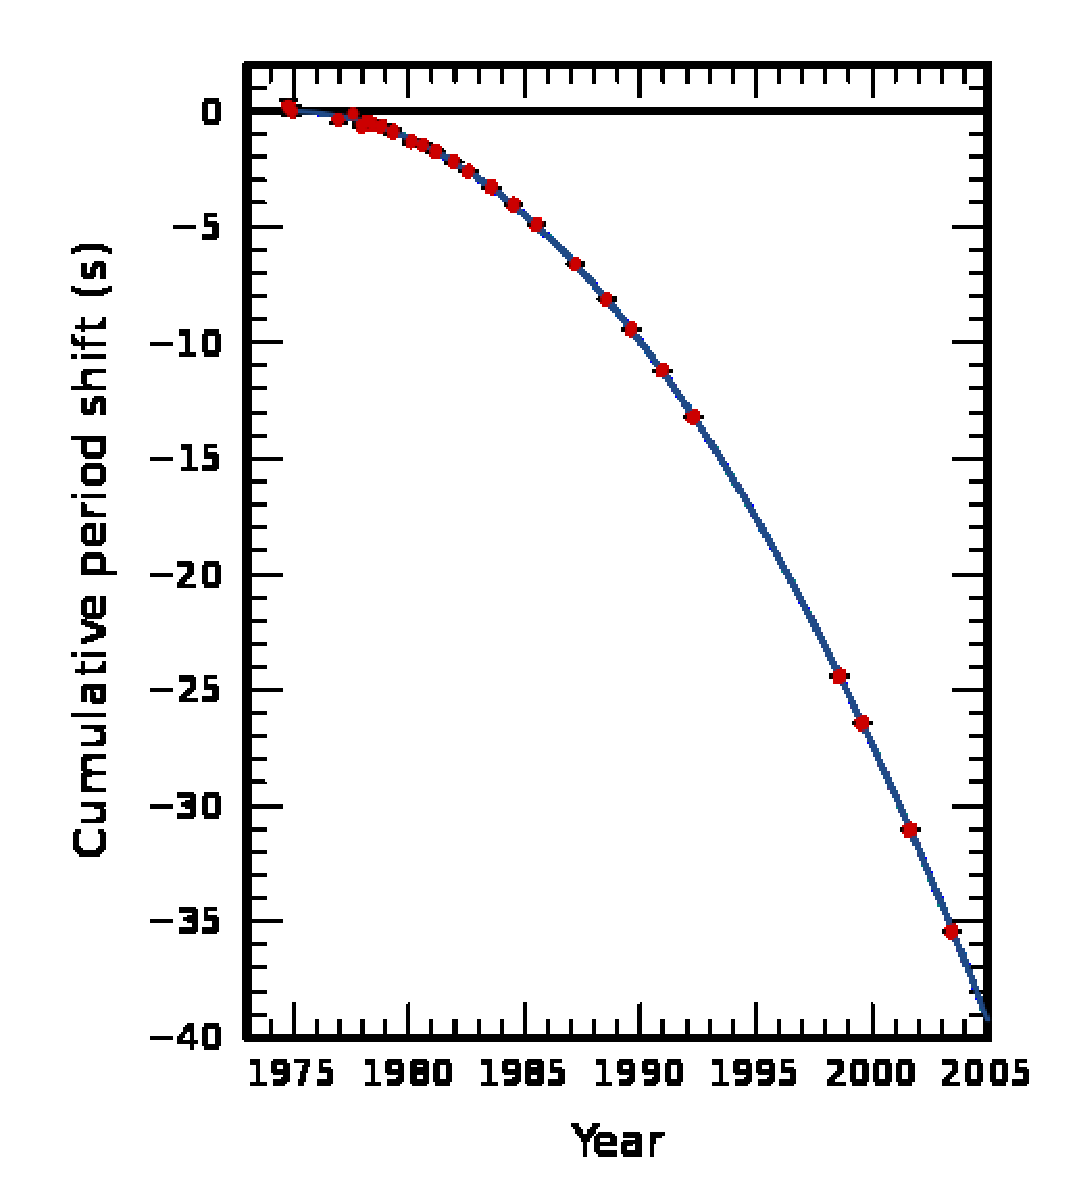
\includegraphics[height=120mm, width=160mm]{500px-PSR_B1913+16_period_shift_graph.eps}
	\caption{The Hulse-Taylor binary, orbital period change over time consistent with emission of gravitational radiation from its system}
	\label{Hulse-Taylor_binary}
	\end{center}
	\end{figure}

		Before delving into the specifics of general relativity, we might consider all the astrophysical sources we expect to emit gravitational waves. Physics prompts our search, but astronomy makes it exciting.

	Discussions of gravitational waves frequently begin with derivations of the wave equations from Einstein's field equations. 
General relativity, however, is not the only theory to predict gravitational waves: waves are a natural consequence of a class of similar theories, which make a range of testable predictions (such as number of polarization modes, from two to six, and possibly speeds different from $c$)~\cite{Will1993} 
Waves should thus be expected even if some minor variation from Einstein's theory is discovered, pointing a way perhaps toward a quantum theory of gravity~\cite{Sathyaprakash2009}. 
As the field progresses toward first detection and beyond to astronomy, the astrophysical targets of our searches should take precedence.

		Gravitational waves (henceforth also abbreviated GW) searches presently focus on four distinct types of cosmic sources.
This categorization of sources was presented in the 1983 LIGO Blue Book proposal and has since guided research focus~\cite{CollinsGravityShadow}. 

This thesis concentrates on continuous waves, which are sine waves -- perhaps modulated by orbital motion, spin-up or spin-down. Continuous waves are most likely to be detectable from neutron stars. Given a sufficiently large ellipticity, which might be on the order of $\epsilon \approx 10^{-6}$ [CITE] or smaller for a neutron star rotating on the order of 1 kHz, a deformation of the crust would radiate sufficient gravitational radiation to be a plausibly-detectable source. Indeed, the radiation would rapidly deplete the rotational energy of the neutron star [CITE], which is why binary systems, where the neutron star could be recycled and spun-up by a partner, prove a promising target [CITE]. Scorpius X-1 offers a canonical case, although our discussion of the TwoSpect analysis will elaborate the abundance of other low-mass X-ray binary (LMXB) systems of interest. Given the paucity of information on the interiors of collapsed stellar remnants, direct detection of gravitational waves from neutron stars could prove informative. We might infer details favoring one equation of state [CITE], might extract parameters suggesting the existence of quark stars or gravitars [CITE], and will have an unparalleled peek into the interior of the densest stable three-dimensional objects in the universe. Their simple waveforms might even facilitate the calibration of other types of gravitational wave data [CITE]. From any source, continuous waves are a conceptually-elegant and astronomically-enticing target.

		Yet other sources of gravitational waves, as will be discussed in more detail later, have a comparable pull on our attention. Oft discussed, inspirals or compact binary coalescences occur when two stellar remnants draw nearer in their orbits, radiating gravitational radiation and finally merging in a titanic release of energy. While sometimes invisible -- the merging of black holes in short-hard gamma ray burts (GRBs) proving an exception -- these events compete eagerly with supernovae as the most explosive in the modern universe. Were we to detect them directly with gravitational waves, we would see their waveforms, which in turn can be predicted through post-Newtonian approximation and numerical relativity. As the amplitude would diminish linearly with distance, we would then have standard candles or 'sirens' by which to calibrate and measure the universe. Advanced LIGO may prove sensitive to neutron star-neutron star and stellar mass black hole-neutron star mergers, and, if low-frequency sensitivity is sufficient and the sources exist, to intermediate-mass black holes. Space-based observatories such as the longsuffering Laser Interferometer Space Antenna (LISA), the DeciHertz Gravitational-wave Observatory (DECIGO), Big Bang Observer (BBO) and proposed others could detect supermassive black hole mergers. If fortunate, they would see a low-frequency noise floor due not to seismic vibration, as in LIGO, but to white dwarf binaries throughout the galaxy. Since the waveforms are well-predicted, we could even investigate deviations from general relativity, perhaps seeing new physics in the ringdown of black holes.

		Physical insight could also come from burst searches. Bursts share with inspiral searches the property of looking for a single event, as opposed to a source spread over duration. Burst is a somewhat general term, and analyses for them can sometimes be applied to inspiral or detector characterization tasks as well, yet the immediate focus lies with supernovae and perhaps gamma-ray bursts. Because the waveform is unknown, burst searches rely significantly more on the coincidence between multiple detectors to distinguish signal from noise. Just as with neutrino observations of supernova 1987A, the burst program would hope for a fortuitously nearby cataclysm to be seen simultaneously -- or nearly so, the time of flight indicating a direction -- in a global gravitational-wave detector network. Due to the versatility of this method, some researchers have proposed looking for non-general relativitic terms, such as longitudinal polarization in addition to plus and cross orthogonal polarization. Any detection would be quiet exciting for probing systems still mysterious with electromagnetic and neutrino measurements, and it would help, in conjunction with multi-messenger coordinated searches with those observatories, to ascertain at precisely what speed gravity travels through space-time and to what extent it is attenuated or altered.

The background of space-time itself may itself how interesting physics and gravitational wave signatures. Searches for the stochastic gravitational wave background look not for events but for many months of correlated signals between networks of detectors. In doing so, they hope in particular to see the earliest turbulence of the universe -- long before the cosmic electromagnetic background, now microwaves, was emitted 380000 years after the Big Bang, gravitational waves were travelling unimpeded. While the opacity of the infant cosmos conflates electromagnetic signals from different times and places, the transparency of the universe to gravity means that we might see the inflationary epoch or earlier, the Planck time, in gravitational waves. Unfortunately, this signal is thought to be far below the sensitivity of existing detectors. While LIGO did set a new upper limit on the energy density of gravitational waves, measured as a fraction, $\Omega_{gw}$ of the critical closure density of the universe~\cite{LIGOStochasticNature2009}, the inflationary background at LIGO frequencies is predicted to be about ten orders of magnitude lower. Alternative theories, such as ekpyrotic/cyclic universes, make other predictions, so an anomalously high stochastic background could prove cosmologically significant.

All gravitational waves searches look for something. While the most exciting possibility remains that we will see the unexpected, we think that our present divisions will permit serendipity while efficiently categorizing the computational challenges we do expect. Continuous wave and inspiral methods both search against waveform templates; burst and stochastic have no template and rely on correlation and coincidence. Continuous wave and stochastic analyze weeks, months, even years of data in search of persistant features; inspiral and burst look for transient events. In the abstract dimensions of search groups, we are complete. Our blind spots are in what data we provide to those groups -- in the focus on audio frequencies of tens to a few thousand Hertz at present -- blindness that will in time be rectified by CMB polarization, pulsar-timing and space-based interferometry for low frequencies and possibly by atom interferometry for high frequencies. To appreciate our choice of focus in these nascent days of the field, we must turn back a century to understand its origins in Einstein's mathematics.

        \subsection{History from general relativity}
        \label{history_GR}

            %Historical brief of Einstein.
        Einstein's theory unified a sequence of historical insights. Since 1676, when Roemer used the moons of Jupiter to measure the finite speed of light, just before Newton's 1687 \textit{Principia Mathematica}~\cite{Hawking2002}, the question of gravity's propogation beckoned. 
Bringing together the work of Minkowski and Poincar\'{e}, the 1905 special theory of relativity highlighted the naturalness of the speed of light, but only in 1915, with the presentation of the Einstein field equations of general relativity, did a means to an answer emerge. 
In 1916, Einstein predicted gravitational waves. 
At last, gravity had a theoretical speed: the same as that of electromagnetism, that of light in the vacuum, $c$.
In the linear approximation to the nonlinear theory of general relativity (henceforth GR), the waves were mathematically similar to the waves of electromagnetism, as will be shown in Section~\ref{general_relativity}.
Yet the detectability of the waves, even in principle, would remain an open question for another half century. 
Consult Misner, Thorne, and Wheeler's \textit{Gravitation}~\cite{MisnerThorneWheeler} and Sean Carroll's collected lectures~\cite{Carroll1997}, as well as other history books of the field for an account of the controversy.
Riles review~\cite{Riles2013}.
Gravity's Shadow~\cite{CollinsGravityShadow} for historical controversy,
Gravity's Ghost~\cite{CollinsGravityGhost} for why we do blind injections

Before deriving the answer to the detectability question, a contrast with the situation in other fields of astronomy is in order.

 
        \subsection{Contrast with electromagnetic and particle astronomy}
        \label{contrast_astro}

        With astronomy, detection came first, then theory.

            Contrast with electromagnetism, compare with radio/X-ray/et cetera astro. Can make analogy to radio waves and make note of the ease with which one can operate a small radio telescope, as I did in my thesis~\cite{MeadorsThesis2008}, compared the the difficulty of gravitational wave detection. Muons from space were detected long ago, as in C.D. Anderson's 1949 paper on what was then called the mesotron,~\cite{CDAnderson}. Compare with neutrinos as in the John Bahcall review paper~\cite{NeutrinoReview}, which were a well-established field by the turn of the millenium, including the detection of supernova 1987A. Might be worth comparing to the focus in new neutrino detectors that I had in my research and development work on them~\cite{EBubble2005},~\cite{MeadorsNevis2006}. Even with those detectors, however, astrophysically-oriented detectors could be cross-referenced against terrestrial generators. Bahcall's search for solar neutrinos, which were theoretical in 1964,~\cite{NeutrinosSolarTheoretical}, at least had the certainty that neutrinos had been detected from the Savannah River nuclear reactor. Yet when those solar neutrinos were detected, it a significant confirmation of nuclear theory. General relativity has been established by the 1913+16 pulsar~\cite{WeisbergTaylor2004} and would likely be much boosted by direct detection, and it might reach surprising new insights, analogous to neutrino oscillation found by looking at the solar neutrino spectrum.

    End section by very rapidly deriving wave equation of electricity and magnetism, to lead by example for how we go about GR.
    Note that all physics in min(action),
    introduce metric as inner product
    generally, coordinate transform good

    Let us set geometric, natural units where $1/4\pi\epsilon \rightarrow 1$. 
Let subscript commas indicate ordinary partial derivatives, semicolons covariant derivatives, and assume the Einstein summation convention.
Greek indices indicate four dimensions, Latin indices three.
A space is supplied with a metric tensor, $g_{\mu\nu}$.

    Gravitation as described by general relativity is complex, so let us start with a simpler theory: electromagnetism. The same mathematics that predicts electromagnetic waves (light), which are our means of detecting gravitational waves in LIGO, can then be extended by analogy to gravitational waves.
Modern physical theories are usually described as extremizing an action, $\mathcal{S}$. The action is defined as the integral, over space-time, of a Lagrangian density $\mathcal{L}$. To integrate, the integral generally requires a metric, $g$, which generalizes the notion of an inner product to curved space. In tensor form, $g = g_{\mu\nu}dx^\mu dx^\nu$. Writing the determinant of the metric as $|g| = \det(g)$, the action to be extremized (setting $\delta \mathcal{S}$ to 0) is

\begin{equation}
\mathcal{S} = \int \mathcal{L} \sqrt{-|g|} d^4 x.
\end{equation} 

The question then becomes how we can define the Lagrangian density for different physical theories. In both electromagnetism and gravitation, the quantity is a kind of curvature, contracted from respectively the Maxwell and Ricci tensors. As educated coordinate transformations make a great number of problems simpler -- a theme of the both the feedforward regression and the data analysis presented in later chapters of this thesis -- let us proceed with the derivation in a way that is manifestly covariant under transformations. If desired, one can then extend this treatment to electromagnetism in curved spacetime, such as under the influence of a gravitational wave. 

    Electromagnetism is theoretically defined by a four-form $\textbf{A} = A_\mu \textbf{d} x^\mu$ where $A_\mu$ is a vector potential~\cite{MisnerThorneWheeler} given by $A_\mu = (\phi, -A_x, -A_y, -A_z)$~\cite{GriffithsE}. 
In a given gauge $\phi$, the theory is `gauge symmetric' such that the addition of the differential form $\textbf{d} \phi$ to $\textbf{A}$ does not change the theory. 
This changeless `symmetry', a symmetry in the group $U(1)$, arises because the physics of the theory can be described through the derived Maxwell field tensor $F_{\mu \nu}$, or curvature form $\textbf{F}$:

\begin{eqnarray}
\textbf{F} = d \textbf{A} = (\partial_\mu A_\nu) dx^\mu \wedge dx^\nu = \frac{1}{2} F_{\mu\nu} \textbf{d}x^\mu \wedge \textbf{d}x^\nu, \\
F_{\mu \nu} = A_{\nu,\mu} - A_{\mu,\nu},
\end{eqnarray}

By the usual flat-space definitions of potential for an electric field $E$ and magnetic field $B$, $E_i = -\phi_{,i} - A_{i,0}$, $B_i = \epsilon_{ijk} \partial^j A^k = \epsilon_{ijk} A^{k, j}$ ($\epsilon_{ijk}$ is the Levi-Civita symbol). 
Electrodynamics in curved space are well-studied; many equations can be translated by replacing partial with covariant derivatives.
Therefore, the Maxwell tensor in explicit coordinate form is

\begin{equation}
F_{\mu\nu} =
\left[
\begin{array}{cccc}
0 & E_x & E_y & E_z\\
-E_x & 0 & -B_z & B_y \\
-E_y &  B_z & 0 & -B_x\\
-E_z & -B_y & B_x & 0
\end{array} \right].
\end{equation}

Maxwell's theory then corresponds to the minimization of the action,

\begin{equation}
\mathcal{S} = \int \mathcal{L} d^4 x,
\end{equation}

\noindent for a Lagrangian $\mathcal{L}$ with a stress-energy term for the field itself constrained by an interaction with the current one-form $\textbf{J} = J_\mu \textbf{d} x^\mu$:

\begin{equation}
\mathcal{L} = - \frac{1}{4} F^{\mu \nu} F_{\mu \nu} + J_\mu A^\mu, 
\end{equation}

On a space that admits a Hodge dual, or star operator, $\star$, we can then define the dual to the Maxwell form, $\star \textbf{F}$. 
Maxwellian electromagnetism then is concisely described by extremizing the action to derive the following equations:

\begin{eqnarray}
d \textbf{F} = 0,\\
d \star \textbf{F} = \star \textbf{J}.
\end{eqnarray}  

Applied in flat space and substituting in the explicit coordinate form of the Maxwell tensor, the theory is easily expressed as four familiar first-order differential equations of the $E$ and $B$ fields (cf. the textbook by Jackson~\cite{JacksonEM}):
 
(CHECK SIGNS AND UNITS AND FONTS)

\begin{eqnarray}
E^i_{,i} = \rho,\\
\epsilon^{ijk} E^{k,j} + B^i_{,0} = 0,\\
B^i_{,i} = 0,\\
\epsilon^{ijk} B^{k,j} - E^i_{,0} = J^i.
\end{eqnarray}

Substituting the definitions of $E$ and $B$ in terms of $\textbf{A}$ and specifying the \textit{Lorenz gauge}, where we choose any a vector potential for which $A^\nu_{,\nu} = 0$, 

\begin{equation}
g^{\mu\nu}A^\sigma_{,\mu\nu} = -J^\sigma,
\end{equation}
        
\noindent often written as $\Box A^\sigma = -J^\sigma$ -- a wave equation. Our task now is to compare with general relativity to see whether a similar wave equation will emerge.

    \section{General relativity}
    \label{general_relativity}

        General relativity (the mathematics). The ideal reference here is Sean Carroll's lecture notes on general relativity,~\cite{Carroll1997}, although I should also cite Will Farr's thesis~\cite{FarrThesis} if it is elegant. Farr is good for citing things like the Palatini action. Of course, I should also "dig down" and cite the original sources that they reference too, where applicable. Can also cite Misner, Thorne and Wheeler~\cite{MisnerThorneWheeler}.

            Introduce the metric $g$ here, but reinforce that it is not essential.
Intro to GR -- right motivation is least action Ricci tensor, implying field equation and phase/time-of-flight implying interferometry.

        \subsection{Symmetry and action principles}
        \label{principles}

            Like electricity and magnetism, GR is the product of symmetry, action. This is the right place for~\cite{Carroll1997}.


        \subsection{Derivation of field equations}
        \label{field_equations}

            A common approach to gravitational wave derivations is linearized gravity~\cite{FlanaganHughes2005}.
            This approach is correct in weak fields, and proceeds~\cite{AdhikariThesis} from the metric $g$ approximation as the sum of a Minkowski (flat spacetime) component, $\eta$, plus a perturbation $h$, where $|h| \ll |\eta|$:

\begin{equation}
g_{\mu \nu} \approx \eta_{\mu \nu} + h_{\mu \nu},
\end{equation}

\noindent leading to a wave equation,

\begin{equation}
-\frac{1}{2} \Box \left(h_{\mu \nu} - \frac{1}{2} \eta_{\mu \nu} h_{\lambda}^{\lambda} \right) = \frac{8 \pi G}{c^4} T_{\mu \nu}.
\end{equation}

The wave carries energy~\cite{BallmerThesis} as well:

\begin{eqnarray}
\rho_{\textup{gw}} = \frac{c^2}{16 \pi G} \left\langle |\partial_t h_+|^2 + |\partial_t h_\times|^2 \right\rangle,\\
P = \frac{G}{5c^5}\left\langle \left( \partial_t^3 I_{ij}\right)^2  \right\rangle \approx 5.5\times 10^{-54} W^{-1} \left\langle \left( \partial_t^3 I_{ij}\right)^2  \right\rangle.
\end{eqnarray}

Let us demonstrate this result and also derive field equations from extremized curvature.

		It's all about the Ricci tensor and the Einstein-Hilbert action. This might be the right place for~\cite{FarrThesis} and other sources.

        \subsection{Radiation from quadrupoles}
        \label{radiation}
  
            Predict power from rotating quadrupole. Might also be a good place to invoke Vladimir's thesis~\cite{DergachevThesis} as well as original primary sources. Note that just as light travels at the speed of light, which is measureable~\cite{CODATA} and which can be derived from electromagnetic theory~\cite{GriffithsE}, so we think that gravity should travel at the speed of light. Note that this radiation should not be affected by the interstellar medium. I think that Ostriker is the source to reference on the ISM~\cite{Caldwell1981},~\cite{McKee1977}.

    \section{Astrophysical estimates}
    \label{estimates}

        Astrophysical estimates and predictions.

        \subsection{Sources: burst, continuous, inspiral and stochastic}
        \label{source_types}

            Describe the four types of sources: burst, continuous, inspiral and stochastic.

            UNLIKE the earlier introduction, which should be able why the sources are interesting, this should summarize, more briefly, the current state of the art in each search. Refers to KEITH's REVIEW PAPER as needed~\cite{Riles2013}.

		Mostly above, but clarify exact how much we should see. Cite the 2009 Nature stochastic paper et al~\cite{LIGOStochasticNature2009}. The importance to early universe cosmology was initially handled by Maggiore~\cite{Maggiore2000}. Before that, of course, once can reference the Allen and Romano methods paper~\cite{Allen1999}, anything interesting from Nick Fotopoulos's thesis~\cite{FotopoulosThesis}, and the various mid-2000s stochastic work that I was familiar with~\cite{Abbott2006},~\cite{Abbott2007}. Note the interesting meaning of anisotropies~\cite{Allen1997} and point out how not only Stefan's radiometer search can find them but how it can be adapted to many other purposes, such as spherical harmonics, which is useful for the cosmic microwave background~\cite{Muciaccia1997} and was briefly my work~\cite{MeadorsCaltech2007} and the Scorpius X-1 search; Stefan's canonical radiometer reference is in Classical Quantum Gravity~\cite{Radiometer2006}.

        \subsection{Continuous waves from neutron stars}
        \label{continuous_waves}

            Continuous -- specifically, binary neutron stars and rate predictions. Describe archetypical search methods as in the 1998 analysis paper~\cite{Jaranowski1998}, the Abbott et al paper~\cite{LSCPulsar2006}, including StackSlide~\cite{LSCPulsarS4}, Einstein at Home~\cite{LSCEinsteinHome2009}, and the most interesting to date from Michigan, Vladimir's PowerFlux~\cite{LSCPowerFlux2009}. Discuss earlier results from the earliest period~\cite{Abbott2004} and an early search for Scorpius X-1~\cite{AbbottPulsar2006}. Reinhard Prix is probably another good source~\cite{Prix2006}.

		Rates go in here.
        The emission mechanism of gravitational radiation with amplitude $h_0$ from a neutron star is is from an elliptical deformation, ellipticity $\epsilon$, on its surface, leading to a quadrupole moment $I$~\cite{LSCPulsar2006} and thus emission at frequency $f = 2\nu$, twice the neutron star spin frequency $\nu$:

        \begin{eqnarray}
        \epsilon = \frac{I_{xx} - I_{yy}}{I_zz}, \\
        h_0 = \frac{4 \pi^2 G}{c^4} \frac{I_{zz} f^2}{r} \epsilon.
        \end{eqnarray}

Excepting the case of torque balance in low-mass X-ray binary systems, neutron star rotation frequency will decay due to gravitational radiation, yielding a relationship between the `spindown age'~\cite{Brady1998} $\tau$ and the gravitational radiation amplitude:

        \begin{eqnarray}
        \tau = -f / \dot{f}, \\
        h_0 = \frac{1}{r} \sqrt{\frac{5 G I_{zz}}{2 c^2 \tau}}.
        \end{eqnarray}

	\begin{figure}
	\begin{center}
	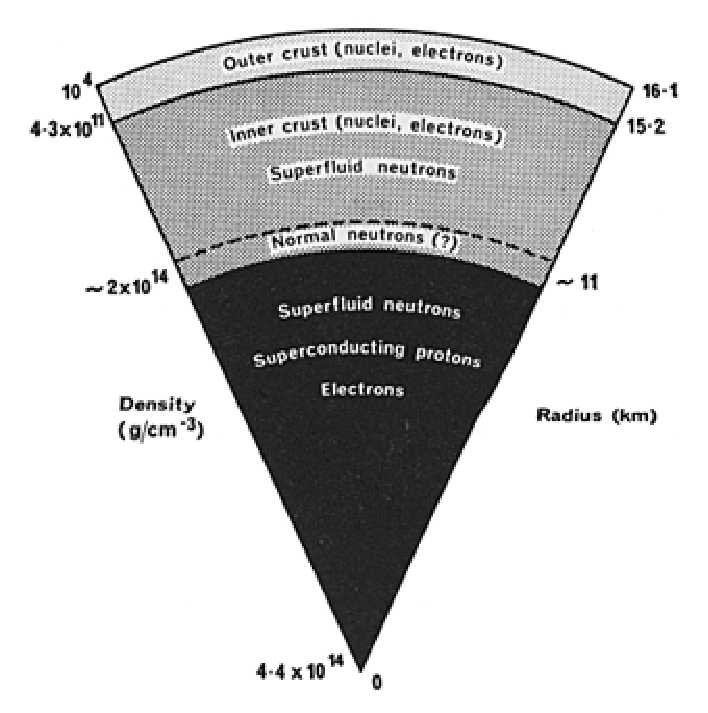
\includegraphics[height=120mm, width=160mm]{neutron_star_structure.eps}
	\caption{Hypothetical internal structure of a neutron star (Citation: http://heasarc.gsfc.nasa.gov/docs/objects/binaries/neutron\_star\_structure.html) CITE? Possibly original Frank Shu? Fred would probably know, being a student of Frank}
	\label{neutron_star_structure}
	\end{center}
	\end{figure}


    \section{Laser Interferometer Gravitational-wave Observatories}
    \label{LIGO}
        
        LIGO observatories. The most fun part to write. Cite Nergis Mavalvala~\cite{MavalvalaThesis}, Stefan Ballmer~\cite{BallmerThesis}, Rana Adhikari~\cite{AdhikariThesis}, Nicolas de Mateo Smith-Lefevbre~\cite{SmithThesis} and, of course, Peter Saulson~\cite{Saulson}.

        \subsection{From Weber bars to interferometry}
        \label{bars_to_interferometry}

            History lesson: Weber bars progress to interferometers. Use Saulson, but Nic's thesis has links to some of the original sources~\cite{Saulson},~\cite{SmithThesis}.           

        \subsection{Observatories, investigations, and enhancements}
        \label{methods}

		Michelson was one of the first to use interferometers~\cite{michelson}. He is famous for having done so to try to measure the velocity of the Earth with respect to the luminerferous ether and finding it to be unmeasurable.

A gravitational wave interferometer, at its core, is also a Michelson interferometer. 
The power $P$ at the output `dark' port, is by design equal to zero except when the measureable (e.g., ether, a gravitational wave, or other disturbance) causes a fringe shift $\Delta \phi$ related to the agnular frequency $\omega$ of the light and the time-of-flight down the $x$ and $y$ arms, $T_x$ and $T_y$. 
Physically, it is proportional to the electric field: 

\begin{eqnarray}
P \propto E_0^2 \left| 1 + e^{i \Delta \phi}\right|^2 = 2 E_0^2 (1 + \cos \Delta \phi), \\
\Delta \phi = \omega (T_y - T_x).
\end{eqnarray}

In Enhanced and Advanced LIGO, $\Delta \phi = 2\pi L_s /\lambda + \phi_0 + \phi_{\textup{DARM}} $, where in decreasing order of size, $L_s$ is known as the Schnupp asymmetry (a constant difference in arm length), $\phi_0$ is a constant offset from a fringe to enable non-radio-frequency-modulated DC readout, and $\phi_{\textup{DARM}}$ is the putative time-varying signal of `DARM', the differential arm motion that might encode a gravitational wave signal. 

Power $P$ can be directly improved by increasing effective laser power (e.g., a brighter laser or use of `power recycling'), and $\delta \phi$ can be increased by making $T_{x,y}$ storage times longer (e.g., with Fabry-Perot cavities).

Gravitational wave signals enter the interferometer, in a technical sense, by changing the spacetime curvature in the arms. It is not necessary to discuss mirror motion or Doppler shifting, although these are also valid points of view. 

In the simplest, linearized picture, the spacetime curvature leads to a gravitational wave with amplitude $h$; when the wave is aligned with x-axis and y-axis arms of length $L$ (see~\cite{Jaranowski1998} for the antenna pattern correction when it is misaligned), it changes the time-of-flight in the arms:

\begin{eqnarray}
T_x = \int_0^{\frac{2L_x}{c}} \sqrt{|g_{xx}|} dt \propto \int_0^{\frac{2L_x}{c}} \left(1 - \frac{h_+}{2} \right) dt, \\
T_y = \int_0^{\frac{2L_y}{c}} \sqrt{|g_{yy}|} dt \propto \int_0^{\frac{2L_y}{c}} \left(1 + \frac{h_+}{2} \right) dt.
\end{eqnarray}

\noindent The mismatch in the integrals leads to a detectable time-varying signal,

\begin{equation}
\phi_{\textup{DARM}} = \omega \int_0^{\frac{2L}{c}} \frac{h_+ (t, x(t)) + h_+ (t, y(t))}{2} dt.
\end{equation}  



            Why GW interferometers work. Null measurements, a zeroed operating point. The specifics are best handled by Saulson~\cite{Saulson}. The idea of a Pound-Drever-Hall lock is most elegantly explained by Black~\cite{PDHNotes}. Rai Weiss may have some neat details, possibly historical, albeit that it is in a presentation~\cite{LIGOWorks}. The details of Fabry-Perot cavities in LIGO are handled by Rakhmanov, Savage et al~\cite{ResonanceFP},~\cite{ResponsesFP}. The motivation for the evolution to Enhanced LIGO and its DC readout methods is covered well in the corresponding CQG article~\cite{Fricke2009} and specific details of its construction and operation are in Tobin Fricke's thesis~\cite{FrickeThesis}.

            \subsubsection{Interferometer theory}
            \label{interferometer_theory}
        
                GW interferometry theory: differential arm motion, key noise sources. Again, the main source is Saulson~\cite{Saulson}, although we also need another source in the Advanced Detector Era.

                Here we discuss the key noises sources: seismic noise, thermal noise, and quantum (radiation pressure, shot noise).

            \subsubsection{Observatory operation}
            \label{observatory_operation}

                Operating LIGO: controls, Detector Characterization. One of the first sources from initial LIGO to read up on is a paper by Fritscel, Bork, Mavalvala et al~\cite{ReadoutGWA}. Initially this system made a detection based on heterodyne readout using gravitational wave sidebands, which, among other troubles, could be unequal in the recycling cavity~\cite{MeadorsHanford2005}.

	\begin{figure}
	\begin{center}
	\includegraphics[height=120mm, width=160mm]{Screen_shot_2010-07-21_at_042516.eps}
	\caption{Screenshot of MEDM control panel}
	\label{ScreenshotMEDM}
	\end{center}
	\end{figure}


                \paragraph{Detector characterization}
                \label{detchar}
            
                    DetChar methods: omega scans, line hunting and glitches

                \paragraph{Feedforward filtering}
                \label{feedforward_filters}

                    Example of feedforward: 60 Hz magnetometer. The only source that mentions this is, I think, Nic's thesis~\cite{SmithThesis}. Yet the most pertinent example is one that has long been applied to LIGO: MICH and PRC feedforward. The specific needed are mention in the thesis of Adhikari~\cite{AdhikariThesis} and Ballmer~\cite{BallmerThesis}, but immediately before Keita Kawabe and I began our project, these parameters had been tuned by Jeff Kissel~\cite{KissellPRCMICH}

	\begin{figure}
	\begin{center}
	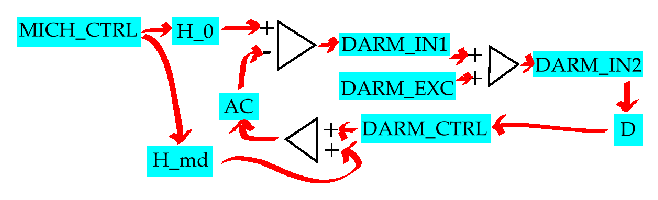
\includegraphics[height=120mm, width=160mm]{servo_loop.eps}
	\caption{Real-time servo loop diagram}
	\label{servo_loop_realtime}
	\end{center}
	\end{figure}

	\begin{figure}
	\begin{center}
	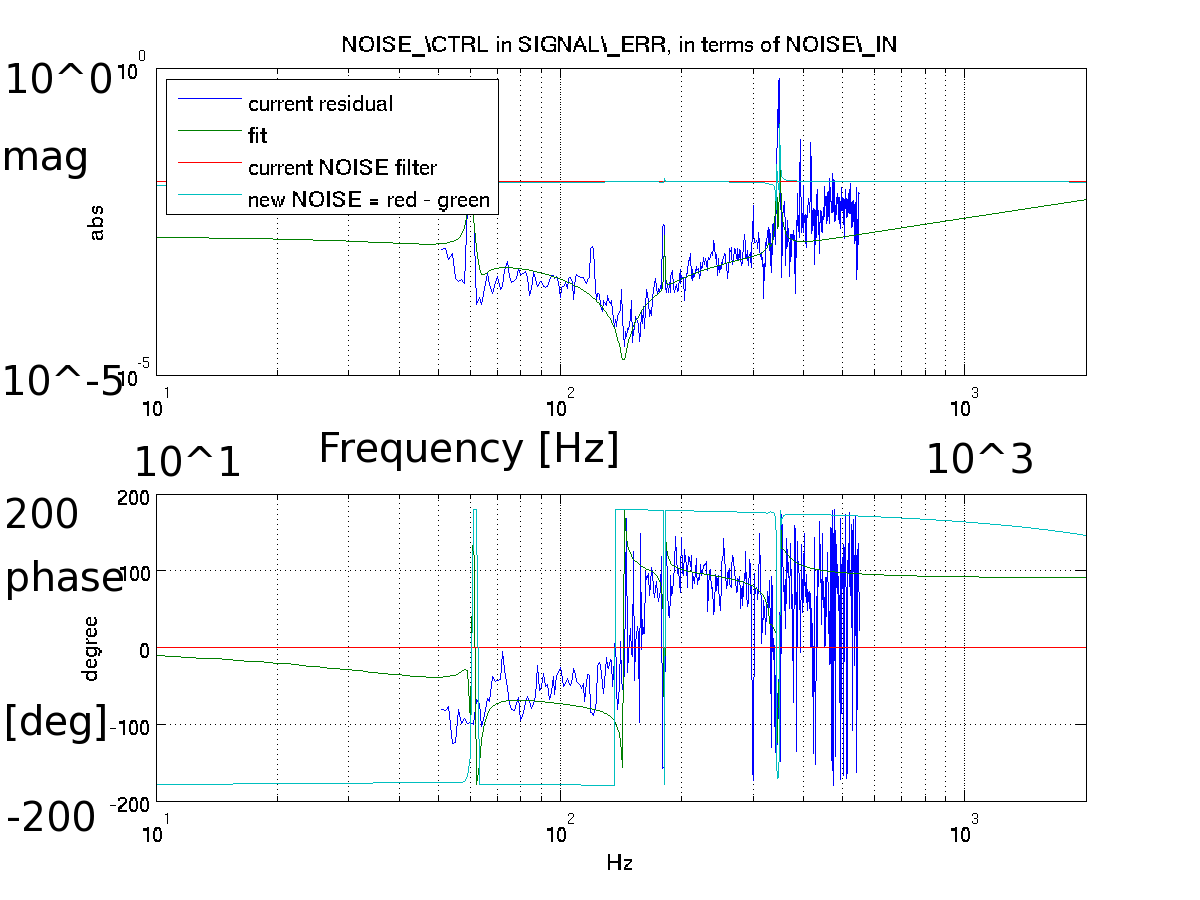
\includegraphics[height=120mm, width=160mm]{newNOISEfilter.eps}
	\caption{Real-time work on a LIGO noise filter}
	\label{newNOISEfilter}
	\end{center}
	\end{figure}

	\begin{figure}
	\begin{center}
	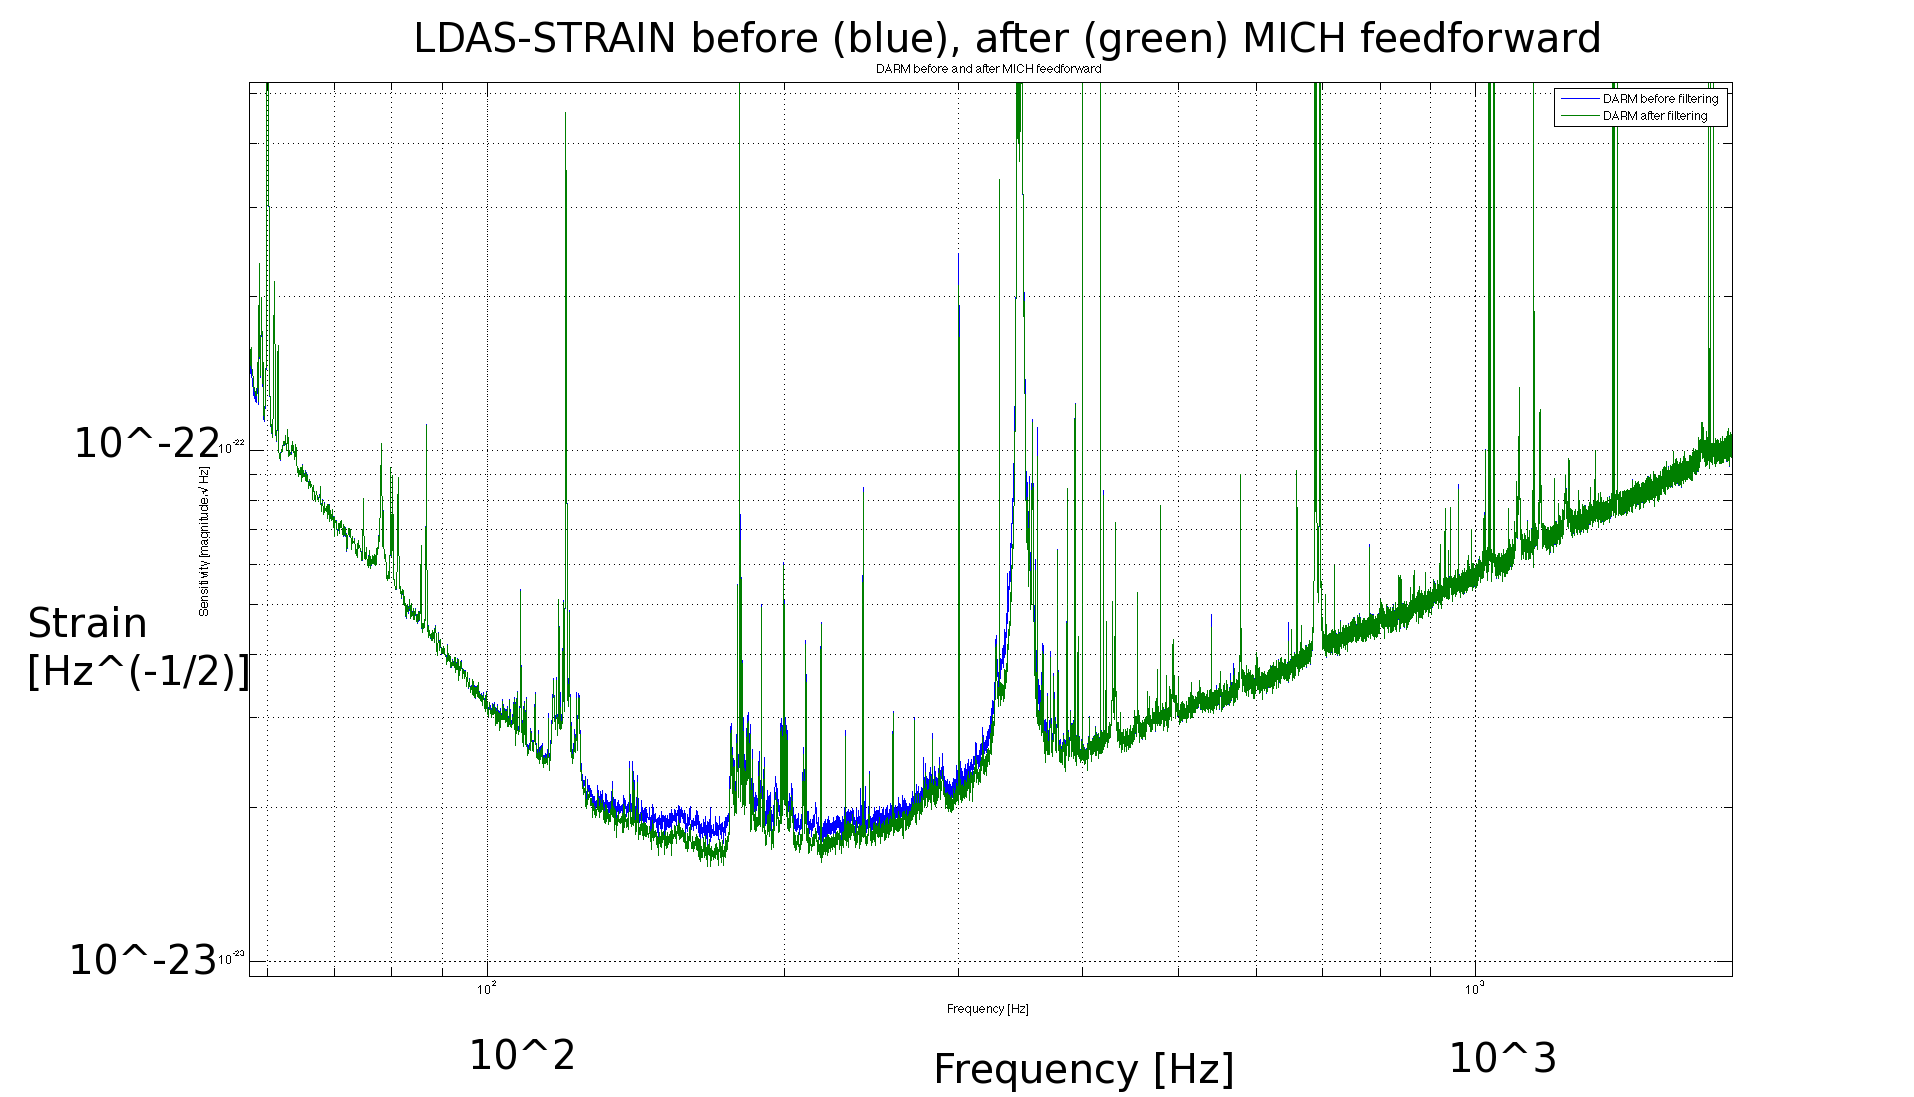
\includegraphics[height=120mm, width=160mm]{2011-03-08_filter-01.eps}
	\caption{Early work on post-facto noise filtering}
	\label{filter_early}
	\end{center}
	\end{figure}

                \paragraph{Phase camera}
                \label{phase_camera}

                    Future devices: overview of phase camera with Vladimir. Vladimir's thesis definitely talks about it~\cite{DergachevThesis}. We can discuss the fundamentals behind the need for angular stabilization and control from Nergis Mavalvala's thesis~\cite{MavalvalaThesis}, but we can refresh it with a modern reference from Kate Dooley's thesis~\cite{DooleyThesis}.


        \subsection{Advanced observatories and beyond}
        \label{advanced}
  
            Advanced LIGO and beyond -- squeezing and prospects?

        \subsection{Worldwide network}
        \label{worldwide}
 
            Allies: LIGO India, KAGRA, Advanced VIRGO, Einstein Telescope, LISA

    \section{Summary}
    \label{intro_summary}
 
        %Summary: strong motivation and instruments, need to find evidence of GW.    

Initial LIGO, during the science runs S6, would have been able to see the coalescence of two neutrons stars at about twenty Megaparsecs, out in the Virgo cluster of galaxies, from sixty-five million years ago, when dinosaurs still walked the Earth. 
In the first week of Advanced LIGO lock at Livingston, following Memorial Day 2014, Advanced LIGO had a temporal range extending only as far back as when early humans began their diaspora from Africa -- a terrestrial parallel to the expansion of the cosmos.
When completed, the Hanford and Livingston second-generation interferometers should see back ten times beyond what S6 could, six hundred and fiften million years, to before the Cambrian explosion of life.
Perhaps in the third or fourth generation of interferometers, our view of the gravitational sky may stretch back the age of the observable universe.
Even then, we will not have seen all that can be seen.
With the two long-range forces of the universe, electromagnetism and gravitational, giving two complimentary views of spacetime, we still must build great machines to explore the sights they show, we must understand what we are seeing, and we must propogate that understanding. 

This thesis is a prelude to those efforts, from the building of the quantum optical squeezer, and the feedforward regression and continuous waves binary search, to our public interferometer exhibitions.   
Feedforward regression provides a microcosm of the complexities of gravitational wave interferometry, so there we will begin.


            
%        --------------------
%
%	Here is a sample chapter file. The chapters of the thesis
%	should be saved to seperate files such as
%	\textit{chapter1.tex}. In the file \textit{thesis.tex} the
%	\textit{input} command then includes these chapters into the
%	thesis. Note that none of the chapter files need any headers.
%	This header for each of these files is contained in
%	\textit{thesis.tex}. The file \textit{thesis.tex} also
%	includes the numbers system for the sections, figures,
%	theorems lemmas etc...

%\section{Sample Section}
%\label{sample_section}
%
%	This is what a sample section looks like. Let's conclude this
%	section with a sample theorem statement and proof.
%
%	\begin{theorem}
%	\label{sample_theorem}
%	The are an infinite number of prime numbers
%	\end{theorem}
%
%	\emph{Proof:} On the contrary assume there are a finite number
%	of primes $P_1, P_2, ... P_n$. Consider $\mathcal{P} = P_1 P_2
%	\cdots P_n+1$. $\mathcal{P}$ is not divisible by any of the
%	primes in our finite set. (Contradiction) $\square$
  

". 


\chapter{Introduction}
\label{intro} 



    \section{Gravitational waves in astrophysics}
    \label{grav_waves_astro}

        Space should reverberate with gravitational waves. 
Light shows part of cosmic history; now, primeval epochs and secret stellar reaches might be seen in patterns of light transformed by gravity. 
General Relativity and related theories of gravitation posit~\cite{EinsteinRosen1937} that changing quadropolar masses radiate gravitationally, just as accelerating dipolar charges do electromagnetically. 
In those waves we might see black holes and neutron stars colliding, supernova, the dawn of the Big Bang and rotating neutron stars -- and the potential for unanticipated insights, into other objects or laws of physics, is too tantalazing to ignore. 
As yet, no direct detections are known. 
Hulse and Taylor \cite{HulseTaylor1975} observed a neutron star in a binary system, PSR 1913+16, with an orbit shrinking just as gravitational radiation would entail. 
Following on the pioneering work of Joseph Weber with bar detectors~\cite{Weber1960} and Robert Forward with tabletop interferometers~\cite{Forward1978}, kilometer-scale interferometers were built at the end of the last millenium to look for gravitational radiation. 
Laser light in these instruments travels orthogonal paths and is reflected back; shifts in the combined pattern are scrutinized for indications that gravitational waves stretched space itself. 
This thesis describes efforts to make that search more sensitive with quantum optics at the observatories, by filtering noise from the data, and by conducting a promising search for continuous waves from neutrons stars in binary systems.

Gravitational wave detectors seek to sense vibrations in the metric of spacetime.
Each chapter in this thesis relates to this endeavor.
LIGO, Virgo, and GEO600, soon to be joined by KAGRA, are kilometer-scale intereferometers, gravitational wave antennae standing on the threshold of detection.
Noise intrinsic to the optical configuration of these instruments is subtracted, as exemplified post-facto by LIGO feedforward filtering using recorded servo data in Chapter \ref{chap2}. 
Sensitivity can also be honed by quantum optical squeezing, selecting the relevant uncertainties from Heisenberg's principle, in Chapter \ref{chap3}.
Astrophysicists expect us to find signals from one of four categories of cosmic sources: inspiralling binary systems of stellar remnants, supernovae and similar bursts, stochastic background, and continuous waves from neutron stars.
Einstein's theory predicts the intensity, speed, and polarization of gravitational waves that could be emitted from these sources.
Low-mass X-ray binaries should lead astronomically long lifetimes, radiating continuous waves from their constituent neutron stars, driving our frequentist search of the Fourier-domain.
Chapters \ref{chap4} and \ref{chap5} use these expectations to enhance and run analyses of simulated and real data, particularly for Scorpius X-1 and XTE J1751-305.
Astronomy has grown from humanity's first glimpses into the night sky with the unaided eye. 
With every new instrument, from Galileo's telescope through radio antennae and neutrino detectors, our understanding of the cosmos has grown. 
Communicating that understanding is the subject of Chapter \ref{chap6}.
Gravity pervades the universe like no other force: we must hear its tale. 

        
        \subsection{Cosmic sources of gravitational waves}
        \label{cosmic_sources}
      
        %   --- Cosmic origins believed to generate GW. (note: should sprinkle citations as needed, not just where it says "cite") ---

		Gravity's power to induce ripples in space is a matter of fact. Pulsar 1913+16, discovered by Hulse and Taylor, not only followed a pattern of orbital decay consistent with radiative loss of orbital decay to gravitational radiation -- it continued to do so~\cite{WeisbergTaylor2004,Weisberg2010}, even after Hulse and Taylor won the 1993 Nobel Prize in physics. 
Moreover, there has been much interest in the question of whether the BICEP2~\cite{BICEP2014} and Planck~\cite{Planck2014} probes of the cosmic microwave background have seen evidence of $B$-mode polarizations that would indicate primordial gravitational fluctuations. We still may ask whether the waves are directly detectable on Earth. We may ask whether they appear in detectors in a way consistent with general relativity. The basic fact of their emission, however, appears settled.

	\begin{figure}
	\begin{center}
	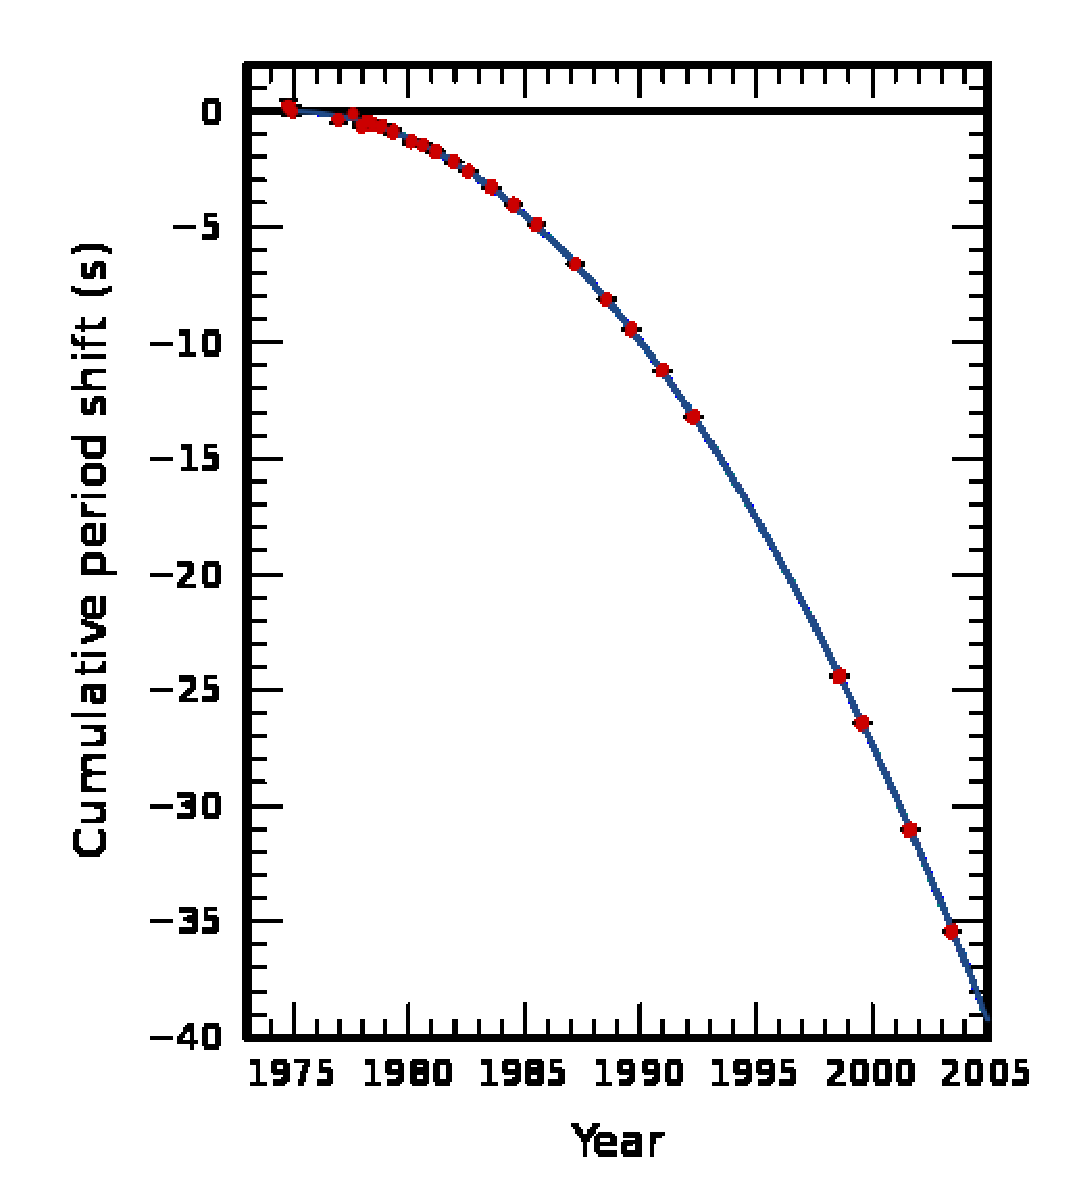
\includegraphics[height=120mm, width=160mm]{500px-PSR_B1913+16_period_shift_graph.eps}
	\caption{The Hulse-Taylor binary, orbital period change over time consistent with emission of gravitational radiation from its system}
	\label{Hulse-Taylor_binary}
	\end{center}
	\end{figure}

		Before delving into the specifics of general relativity, we might consider all the astrophysical sources we expect to emit gravitational waves. Physics prompts our search, but astronomy makes it exciting.

	Discussions of gravitational waves frequently begin with derivations of the wave equations from Einstein's field equations. 
General relativity, however, is not the only theory to predict gravitational waves: waves are a natural consequence of a class of similar theories, which make a range of testable predictions (such as number of polarization modes, from two to six, and possibly speeds different from $c$)~\cite{Will1993} 
Waves should thus be expected even if some minor variation from Einstein's theory is discovered, pointing a way perhaps toward a quantum theory of gravity~\cite{Sathyaprakash2009}. 
As the field progresses toward first detection and beyond to astronomy, the astrophysical targets of our searches should take precedence.

		Gravitational waves (henceforth also abbreviated GW) searches presently focus on four distinct types of cosmic sources.
This categorization of sources was presented in the 1983 LIGO Blue Book proposal and has since guided research focus~\cite{CollinsGravityShadow}. 

This thesis concentrates on continuous waves, which are sine waves -- perhaps modulated by orbital motion, spin-up or spin-down. Continuous waves are most likely to be detectable from neutron stars. Given a sufficiently large ellipticity, which might be on the order of $\epsilon \approx 10^{-6}$ [CITE] or smaller for a neutron star rotating on the order of 1 kHz, a deformation of the crust would radiate sufficient gravitational radiation to be a plausibly-detectable source. Indeed, the radiation would rapidly deplete the rotational energy of the neutron star [CITE], which is why binary systems, where the neutron star could be recycled and spun-up by a partner, prove a promising target [CITE]. Scorpius X-1 offers a canonical case, although our discussion of the TwoSpect analysis will elaborate the abundance of other low-mass X-ray binary (LMXB) systems of interest. Given the paucity of information on the interiors of collapsed stellar remnants, direct detection of gravitational waves from neutron stars could prove informative. We might infer details favoring one equation of state [CITE], might extract parameters suggesting the existence of quark stars or gravitars [CITE], and will have an unparalleled peek into the interior of the densest stable three-dimensional objects in the universe. Their simple waveforms might even facilitate the calibration of other types of gravitational wave data [CITE]. From any source, continuous waves are a conceptually-elegant and astronomically-enticing target.

		Yet other sources of gravitational waves, as will be discussed in more detail later, have a comparable pull on our attention. Oft discussed, inspirals or compact binary coalescences occur when two stellar remnants draw nearer in their orbits, radiating gravitational radiation and finally merging in a titanic release of energy. While sometimes invisible -- the merging of black holes in short-hard gamma ray burts (GRBs) proving an exception -- these events compete eagerly with supernovae as the most explosive in the modern universe. Were we to detect them directly with gravitational waves, we would see their waveforms, which in turn can be predicted through post-Newtonian approximation and numerical relativity. As the amplitude would diminish linearly with distance, we would then have standard candles or 'sirens' by which to calibrate and measure the universe. Advanced LIGO may prove sensitive to neutron star-neutron star and stellar mass black hole-neutron star mergers, and, if low-frequency sensitivity is sufficient and the sources exist, to intermediate-mass black holes. Space-based observatories such as the longsuffering Laser Interferometer Space Antenna (LISA), the DeciHertz Gravitational-wave Observatory (DECIGO), Big Bang Observer (BBO) and proposed others could detect supermassive black hole mergers. If fortunate, they would see a low-frequency noise floor due not to seismic vibration, as in LIGO, but to white dwarf binaries throughout the galaxy. Since the waveforms are well-predicted, we could even investigate deviations from general relativity, perhaps seeing new physics in the ringdown of black holes.

		Physical insight could also come from burst searches. Bursts share with inspiral searches the property of looking for a single event, as opposed to a source spread over duration. Burst is a somewhat general term, and analyses for them can sometimes be applied to inspiral or detector characterization tasks as well, yet the immediate focus lies with supernovae and perhaps gamma-ray bursts. Because the waveform is unknown, burst searches rely significantly more on the coincidence between multiple detectors to distinguish signal from noise. Just as with neutrino observations of supernova 1987A, the burst program would hope for a fortuitously nearby cataclysm to be seen simultaneously -- or nearly so, the time of flight indicating a direction -- in a global gravitational-wave detector network. Due to the versatility of this method, some researchers have proposed looking for non-general relativitic terms, such as longitudinal polarization in addition to plus and cross orthogonal polarization. Any detection would be quiet exciting for probing systems still mysterious with electromagnetic and neutrino measurements, and it would help, in conjunction with multi-messenger coordinated searches with those observatories, to ascertain at precisely what speed gravity travels through space-time and to what extent it is attenuated or altered.

The background of space-time itself may itself how interesting physics and gravitational wave signatures. Searches for the stochastic gravitational wave background look not for events but for many months of correlated signals between networks of detectors. In doing so, they hope in particular to see the earliest turbulence of the universe -- long before the cosmic electromagnetic background, now microwaves, was emitted 380000 years after the Big Bang, gravitational waves were travelling unimpeded. While the opacity of the infant cosmos conflates electromagnetic signals from different times and places, the transparency of the universe to gravity means that we might see the inflationary epoch or earlier, the Planck time, in gravitational waves. Unfortunately, this signal is thought to be far below the sensitivity of existing detectors. While LIGO did set a new upper limit on the energy density of gravitational waves, measured as a fraction, $\Omega_{gw}$ of the critical closure density of the universe~\cite{LIGOStochasticNature2009}, the inflationary background at LIGO frequencies is predicted to be about ten orders of magnitude lower. Alternative theories, such as ekpyrotic/cyclic universes, make other predictions, so an anomalously high stochastic background could prove cosmologically significant.

All gravitational waves searches look for something. While the most exciting possibility remains that we will see the unexpected, we think that our present divisions will permit serendipity while efficiently categorizing the computational challenges we do expect. Continuous wave and inspiral methods both search against waveform templates; burst and stochastic have no template and rely on correlation and coincidence. Continuous wave and stochastic analyze weeks, months, even years of data in search of persistant features; inspiral and burst look for transient events. In the abstract dimensions of search groups, we are complete. Our blind spots are in what data we provide to those groups -- in the focus on audio frequencies of tens to a few thousand Hertz at present -- blindness that will in time be rectified by CMB polarization, pulsar-timing and space-based interferometry for low frequencies and possibly by atom interferometry for high frequencies. To appreciate our choice of focus in these nascent days of the field, we must turn back a century to understand its origins in Einstein's mathematics.

        \subsection{History from general relativity}
        \label{history_GR}

            %Historical brief of Einstein.
        Einstein's theory unified a sequence of historical insights. Since 1676, when Roemer used the moons of Jupiter to measure the finite speed of light, just before Newton's 1687 \textit{Principia Mathematica}~\cite{Hawking2002}, the question of gravity's propogation beckoned. 
Bringing together the work of Minkowski and Poincar\'{e}, the 1905 special theory of relativity highlighted the naturalness of the speed of light, but only in 1915, with the presentation of the Einstein field equations of general relativity, did a means to an answer emerge. 
In 1916, Einstein predicted gravitational waves. 
At last, gravity had a theoretical speed: the same as that of electromagnetism, that of light in the vacuum, $c$.
In the linear approximation to the nonlinear theory of general relativity (henceforth GR), the waves were mathematically similar to the waves of electromagnetism, as will be shown in Section~\ref{general_relativity}.
Yet the detectability of the waves, even in principle, would remain an open question for another half century. 
Consult Misner, Thorne, and Wheeler's \textit{Gravitation}~\cite{MisnerThorneWheeler} and Sean Carroll's collected lectures~\cite{Carroll1997}, as well as other history books of the field for an account of the controversy.
Riles review~\cite{Riles2013}.
Gravity's Shadow~\cite{CollinsGravityShadow} for historical controversy,
Gravity's Ghost~\cite{CollinsGravityGhost} for why we do blind injections

Before deriving the answer to the detectability question, a contrast with the situation in other fields of astronomy is in order.

 
        \subsection{Contrast with electromagnetic and particle astronomy}
        \label{contrast_astro}

        With astronomy, detection came first, then theory.

            Contrast with electromagnetism, compare with radio/X-ray/et cetera astro. Can make analogy to radio waves and make note of the ease with which one can operate a small radio telescope, as I did in my thesis~\cite{MeadorsThesis2008}, compared the the difficulty of gravitational wave detection. Muons from space were detected long ago, as in C.D. Anderson's 1949 paper on what was then called the mesotron,~\cite{CDAnderson}. Compare with neutrinos as in the John Bahcall review paper~\cite{NeutrinoReview}, which were a well-established field by the turn of the millenium, including the detection of supernova 1987A. Might be worth comparing to the focus in new neutrino detectors that I had in my research and development work on them~\cite{EBubble2005},~\cite{MeadorsNevis2006}. Even with those detectors, however, astrophysically-oriented detectors could be cross-referenced against terrestrial generators. Bahcall's search for solar neutrinos, which were theoretical in 1964,~\cite{NeutrinosSolarTheoretical}, at least had the certainty that neutrinos had been detected from the Savannah River nuclear reactor. Yet when those solar neutrinos were detected, it a significant confirmation of nuclear theory. General relativity has been established by the 1913+16 pulsar~\cite{WeisbergTaylor2004} and would likely be much boosted by direct detection, and it might reach surprising new insights, analogous to neutrino oscillation found by looking at the solar neutrino spectrum.

    End section by very rapidly deriving wave equation of electricity and magnetism, to lead by example for how we go about GR.
    Note that all physics in min(action),
    introduce metric as inner product
    generally, coordinate transform good

    Let us set geometric, natural units where $1/4\pi\epsilon \rightarrow 1$. 
Let subscript commas indicate ordinary partial derivatives, semicolons covariant derivatives, and assume the Einstein summation convention.
Greek indices indicate four dimensions, Latin indices three.
A space is supplied with a metric tensor, $g_{\mu\nu}$.

    Gravitation as described by general relativity is complex, so let us start with a simpler theory: electromagnetism. The same mathematics that predicts electromagnetic waves (light), which are our means of detecting gravitational waves in LIGO, can then be extended by analogy to gravitational waves.
Modern physical theories are usually described as extremizing an action, $\mathcal{S}$. The action is defined as the integral, over space-time, of a Lagrangian density $\mathcal{L}$. To integrate, the integral generally requires a metric, $g$, which generalizes the notion of an inner product to curved space. In tensor form, $g = g_{\mu\nu}dx^\mu dx^\nu$. Writing the determinant of the metric as $|g| = \det(g)$, the action to be extremized (setting $\delta \mathcal{S}$ to 0) is

\begin{equation}
\mathcal{S} = \int \mathcal{L} \sqrt{-|g|} d^4 x.
\end{equation} 

The question then becomes how we can define the Lagrangian density for different physical theories. In both electromagnetism and gravitation, the quantity is a kind of curvature, contracted from respectively the Maxwell and Ricci tensors. As educated coordinate transformations make a great number of problems simpler -- a theme of the both the feedforward regression and the data analysis presented in later chapters of this thesis -- let us proceed with the derivation in a way that is manifestly covariant under transformations. If desired, one can then extend this treatment to electromagnetism in curved spacetime, such as under the influence of a gravitational wave. 

    Electromagnetism is theoretically defined by a four-form $\textbf{A} = A_\mu \textbf{d} x^\mu$ where $A_\mu$ is a vector potential~\cite{MisnerThorneWheeler} given by $A_\mu = (\phi, -A_x, -A_y, -A_z)$~\cite{GriffithsE}. 
In a given gauge $\phi$, the theory is `gauge symmetric' such that the addition of the differential form $\textbf{d} \phi$ to $\textbf{A}$ does not change the theory. 
This changeless `symmetry', a symmetry in the group $U(1)$, arises because the physics of the theory can be described through the derived Maxwell field tensor $F_{\mu \nu}$, or curvature form $\textbf{F}$:

\begin{eqnarray}
\textbf{F} = d \textbf{A} = (\partial_\mu A_\nu) dx^\mu \wedge dx^\nu = \frac{1}{2} F_{\mu\nu} \textbf{d}x^\mu \wedge \textbf{d}x^\nu, \\
F_{\mu \nu} = A_{\nu,\mu} - A_{\mu,\nu},
\end{eqnarray}

By the usual flat-space definitions of potential for an electric field $E$ and magnetic field $B$, $E_i = -\phi_{,i} - A_{i,0}$, $B_i = \epsilon_{ijk} \partial^j A^k = \epsilon_{ijk} A^{k, j}$ ($\epsilon_{ijk}$ is the Levi-Civita symbol). 
Electrodynamics in curved space are well-studied; many equations can be translated by replacing partial with covariant derivatives.
Therefore, the Maxwell tensor in explicit coordinate form is

\begin{equation}
F_{\mu\nu} =
\left[
\begin{array}{cccc}
0 & E_x & E_y & E_z\\
-E_x & 0 & -B_z & B_y \\
-E_y &  B_z & 0 & -B_x\\
-E_z & -B_y & B_x & 0
\end{array} \right].
\end{equation}

Maxwell's theory then corresponds to the minimization of the action,

\begin{equation}
\mathcal{S} = \int \mathcal{L} d^4 x,
\end{equation}

\noindent for a Lagrangian $\mathcal{L}$ with a stress-energy term for the field itself constrained by an interaction with the current one-form $\textbf{J} = J_\mu \textbf{d} x^\mu$:

\begin{equation}
\mathcal{L} = - \frac{1}{4} F^{\mu \nu} F_{\mu \nu} + J_\mu A^\mu, 
\end{equation}

On a space that admits a Hodge dual, or star operator, $\star$, we can then define the dual to the Maxwell form, $\star \textbf{F}$. 
Maxwellian electromagnetism then is concisely described by extremizing the action to derive the following equations:

\begin{eqnarray}
d \textbf{F} = 0,\\
d \star \textbf{F} = \star \textbf{J}.
\end{eqnarray}  

Applied in flat space and substituting in the explicit coordinate form of the Maxwell tensor, the theory is easily expressed as four familiar first-order differential equations of the $E$ and $B$ fields (cf. the textbook by Jackson~\cite{JacksonEM}):
 
(CHECK SIGNS AND UNITS AND FONTS)

\begin{eqnarray}
E^i_{,i} = \rho,\\
\epsilon^{ijk} E^{k,j} + B^i_{,0} = 0,\\
B^i_{,i} = 0,\\
\epsilon^{ijk} B^{k,j} - E^i_{,0} = J^i.
\end{eqnarray}

Substituting the definitions of $E$ and $B$ in terms of $\textbf{A}$ and specifying the \textit{Lorenz gauge}, where we choose any a vector potential for which $A^\nu_{,\nu} = 0$, 

\begin{equation}
g^{\mu\nu}A^\sigma_{,\mu\nu} = -J^\sigma,
\end{equation}
        
\noindent often written as $\Box A^\sigma = -J^\sigma$ -- a wave equation. Our task now is to compare with general relativity to see whether a similar wave equation will emerge.

    \section{General relativity}
    \label{general_relativity}

        General relativity (the mathematics). The ideal reference here is Sean Carroll's lecture notes on general relativity,~\cite{Carroll1997}, although I should also cite Will Farr's thesis~\cite{FarrThesis} if it is elegant. Farr is good for citing things like the Palatini action. Of course, I should also "dig down" and cite the original sources that they reference too, where applicable. Can also cite Misner, Thorne and Wheeler~\cite{MisnerThorneWheeler}.

            Introduce the metric $g$ here, but reinforce that it is not essential.
Intro to GR -- right motivation is least action Ricci tensor, implying field equation and phase/time-of-flight implying interferometry.

        \subsection{Symmetry and action principles}
        \label{principles}

            Like electricity and magnetism, GR is the product of symmetry, action. This is the right place for~\cite{Carroll1997}.


        \subsection{Derivation of field equations}
        \label{field_equations}

            A common approach to gravitational wave derivations is linearized gravity~\cite{FlanaganHughes2005}.
            This approach is correct in weak fields, and proceeds~\cite{AdhikariThesis} from the metric $g$ approximation as the sum of a Minkowski (flat spacetime) component, $\eta$, plus a perturbation $h$, where $|h| \ll |\eta|$:

\begin{equation}
g_{\mu \nu} \approx \eta_{\mu \nu} + h_{\mu \nu},
\end{equation}

\noindent leading to a wave equation,

\begin{equation}
-\frac{1}{2} \Box \left(h_{\mu \nu} - \frac{1}{2} \eta_{\mu \nu} h_{\lambda}^{\lambda} \right) = \frac{8 \pi G}{c^4} T_{\mu \nu}.
\end{equation}

The wave carries energy~\cite{BallmerThesis} as well:

\begin{eqnarray}
\rho_{\textup{gw}} = \frac{c^2}{16 \pi G} \left\langle |\partial_t h_+|^2 + |\partial_t h_\times|^2 \right\rangle,\\
P = \frac{G}{5c^5}\left\langle \left( \partial_t^3 I_{ij}\right)^2  \right\rangle \approx 5.5\times 10^{-54} W^{-1} \left\langle \left( \partial_t^3 I_{ij}\right)^2  \right\rangle.
\end{eqnarray}

Let us demonstrate this result and also derive field equations from extremized curvature.

		It's all about the Ricci tensor and the Einstein-Hilbert action. This might be the right place for~\cite{FarrThesis} and other sources.

        \subsection{Radiation from quadrupoles}
        \label{radiation}
  
            Predict power from rotating quadrupole. Might also be a good place to invoke Vladimir's thesis~\cite{DergachevThesis} as well as original primary sources. Note that just as light travels at the speed of light, which is measureable~\cite{CODATA} and which can be derived from electromagnetic theory~\cite{GriffithsE}, so we think that gravity should travel at the speed of light. Note that this radiation should not be affected by the interstellar medium. I think that Ostriker is the source to reference on the ISM~\cite{Caldwell1981},~\cite{McKee1977}.

    \section{Astrophysical estimates}
    \label{estimates}

        Astrophysical estimates and predictions.

        \subsection{Sources: burst, continuous, inspiral and stochastic}
        \label{source_types}

            Describe the four types of sources: burst, continuous, inspiral and stochastic.

            UNLIKE the earlier introduction, which should be able why the sources are interesting, this should summarize, more briefly, the current state of the art in each search. Refers to KEITH's REVIEW PAPER as needed~\cite{Riles2013}.

		Mostly above, but clarify exact how much we should see. Cite the 2009 Nature stochastic paper et al~\cite{LIGOStochasticNature2009}. The importance to early universe cosmology was initially handled by Maggiore~\cite{Maggiore2000}. Before that, of course, once can reference the Allen and Romano methods paper~\cite{Allen1999}, anything interesting from Nick Fotopoulos's thesis~\cite{FotopoulosThesis}, and the various mid-2000s stochastic work that I was familiar with~\cite{Abbott2006},~\cite{Abbott2007}. Note the interesting meaning of anisotropies~\cite{Allen1997} and point out how not only Stefan's radiometer search can find them but how it can be adapted to many other purposes, such as spherical harmonics, which is useful for the cosmic microwave background~\cite{Muciaccia1997} and was briefly my work~\cite{MeadorsCaltech2007} and the Scorpius X-1 search; Stefan's canonical radiometer reference is in Classical Quantum Gravity~\cite{Radiometer2006}.

        \subsection{Continuous waves from neutron stars}
        \label{continuous_waves}

            Continuous -- specifically, binary neutron stars and rate predictions. Describe archetypical search methods as in the 1998 analysis paper~\cite{Jaranowski1998}, the Abbott et al paper~\cite{LSCPulsar2006}, including StackSlide~\cite{LSCPulsarS4}, Einstein at Home~\cite{LSCEinsteinHome2009}, and the most interesting to date from Michigan, Vladimir's PowerFlux~\cite{LSCPowerFlux2009}. Discuss earlier results from the earliest period~\cite{Abbott2004} and an early search for Scorpius X-1~\cite{AbbottPulsar2006}. Reinhard Prix is probably another good source~\cite{Prix2006}.

		Rates go in here.
        The emission mechanism of gravitational radiation with amplitude $h_0$ from a neutron star is is from an elliptical deformation, ellipticity $\epsilon$, on its surface, leading to a quadrupole moment $I$~\cite{LSCPulsar2006} and thus emission at frequency $f = 2\nu$, twice the neutron star spin frequency $\nu$:

        \begin{eqnarray}
        \epsilon = \frac{I_{xx} - I_{yy}}{I_zz}, \\
        h_0 = \frac{4 \pi^2 G}{c^4} \frac{I_{zz} f^2}{r} \epsilon.
        \end{eqnarray}

Excepting the case of torque balance in low-mass X-ray binary systems, neutron star rotation frequency will decay due to gravitational radiation, yielding a relationship between the `spindown age'~\cite{Brady1998} $\tau$ and the gravitational radiation amplitude:

        \begin{eqnarray}
        \tau = -f / \dot{f}, \\
        h_0 = \frac{1}{r} \sqrt{\frac{5 G I_{zz}}{2 c^2 \tau}}.
        \end{eqnarray}

	\begin{figure}
	\begin{center}
	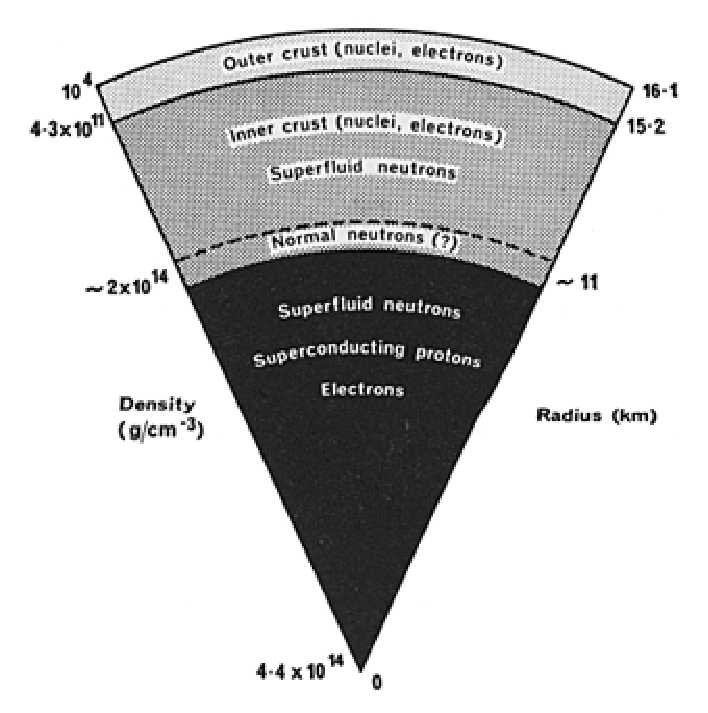
\includegraphics[height=120mm, width=160mm]{neutron_star_structure.eps}
	\caption{Hypothetical internal structure of a neutron star (Citation: http://heasarc.gsfc.nasa.gov/docs/objects/binaries/neutron\_star\_structure.html) CITE? Possibly original Frank Shu? Fred would probably know, being a student of Frank}
	\label{neutron_star_structure}
	\end{center}
	\end{figure}


    \section{Laser Interferometer Gravitational-wave Observatories}
    \label{LIGO}
        
        LIGO observatories. The most fun part to write. Cite Nergis Mavalvala~\cite{MavalvalaThesis}, Stefan Ballmer~\cite{BallmerThesis}, Rana Adhikari~\cite{AdhikariThesis}, Nicolas de Mateo Smith-Lefevbre~\cite{SmithThesis} and, of course, Peter Saulson~\cite{Saulson}.

        \subsection{From Weber bars to interferometry}
        \label{bars_to_interferometry}

            History lesson: Weber bars progress to interferometers. Use Saulson, but Nic's thesis has links to some of the original sources~\cite{Saulson},~\cite{SmithThesis}.           

        \subsection{Observatories, investigations, and enhancements}
        \label{methods}

		Michelson was one of the first to use interferometers~\cite{michelson}. He is famous for having done so to try to measure the velocity of the Earth with respect to the luminerferous ether and finding it to be unmeasurable.

A gravitational wave interferometer, at its core, is also a Michelson interferometer. 
The power $P$ at the output `dark' port, is by design equal to zero except when the measureable (e.g., ether, a gravitational wave, or other disturbance) causes a fringe shift $\Delta \phi$ related to the agnular frequency $\omega$ of the light and the time-of-flight down the $x$ and $y$ arms, $T_x$ and $T_y$. 
Physically, it is proportional to the electric field: 

\begin{eqnarray}
P \propto E_0^2 \left| 1 + e^{i \Delta \phi}\right|^2 = 2 E_0^2 (1 + \cos \Delta \phi), \\
\Delta \phi = \omega (T_y - T_x).
\end{eqnarray}

In Enhanced and Advanced LIGO, $\Delta \phi = 2\pi L_s /\lambda + \phi_0 + \phi_{\textup{DARM}} $, where in decreasing order of size, $L_s$ is known as the Schnupp asymmetry (a constant difference in arm length), $\phi_0$ is a constant offset from a fringe to enable non-radio-frequency-modulated DC readout, and $\phi_{\textup{DARM}}$ is the putative time-varying signal of `DARM', the differential arm motion that might encode a gravitational wave signal. 

Power $P$ can be directly improved by increasing effective laser power (e.g., a brighter laser or use of `power recycling'), and $\delta \phi$ can be increased by making $T_{x,y}$ storage times longer (e.g., with Fabry-Perot cavities).

Gravitational wave signals enter the interferometer, in a technical sense, by changing the spacetime curvature in the arms. It is not necessary to discuss mirror motion or Doppler shifting, although these are also valid points of view. 

In the simplest, linearized picture, the spacetime curvature leads to a gravitational wave with amplitude $h$; when the wave is aligned with x-axis and y-axis arms of length $L$ (see~\cite{Jaranowski1998} for the antenna pattern correction when it is misaligned), it changes the time-of-flight in the arms:

\begin{eqnarray}
T_x = \int_0^{\frac{2L_x}{c}} \sqrt{|g_{xx}|} dt \propto \int_0^{\frac{2L_x}{c}} \left(1 - \frac{h_+}{2} \right) dt, \\
T_y = \int_0^{\frac{2L_y}{c}} \sqrt{|g_{yy}|} dt \propto \int_0^{\frac{2L_y}{c}} \left(1 + \frac{h_+}{2} \right) dt.
\end{eqnarray}

\noindent The mismatch in the integrals leads to a detectable time-varying signal,

\begin{equation}
\phi_{\textup{DARM}} = \omega \int_0^{\frac{2L}{c}} \frac{h_+ (t, x(t)) + h_+ (t, y(t))}{2} dt.
\end{equation}  



            Why GW interferometers work. Null measurements, a zeroed operating point. The specifics are best handled by Saulson~\cite{Saulson}. The idea of a Pound-Drever-Hall lock is most elegantly explained by Black~\cite{PDHNotes}. Rai Weiss may have some neat details, possibly historical, albeit that it is in a presentation~\cite{LIGOWorks}. The details of Fabry-Perot cavities in LIGO are handled by Rakhmanov, Savage et al~\cite{ResonanceFP},~\cite{ResponsesFP}. The motivation for the evolution to Enhanced LIGO and its DC readout methods is covered well in the corresponding CQG article~\cite{Fricke2009} and specific details of its construction and operation are in Tobin Fricke's thesis~\cite{FrickeThesis}.

            \subsubsection{Interferometer theory}
            \label{interferometer_theory}
        
                GW interferometry theory: differential arm motion, key noise sources. Again, the main source is Saulson~\cite{Saulson}, although we also need another source in the Advanced Detector Era.

                Here we discuss the key noises sources: seismic noise, thermal noise, and quantum (radiation pressure, shot noise).

            \subsubsection{Observatory operation}
            \label{observatory_operation}

                Operating LIGO: controls, Detector Characterization. One of the first sources from initial LIGO to read up on is a paper by Fritscel, Bork, Mavalvala et al~\cite{ReadoutGWA}. Initially this system made a detection based on heterodyne readout using gravitational wave sidebands, which, among other troubles, could be unequal in the recycling cavity~\cite{MeadorsHanford2005}.

	\begin{figure}
	\begin{center}
	\includegraphics[height=120mm, width=160mm]{Screen_shot_2010-07-21_at_042516.eps}
	\caption{Screenshot of MEDM control panel}
	\label{ScreenshotMEDM}
	\end{center}
	\end{figure}


                \paragraph{Detector characterization}
                \label{detchar}
            
                    DetChar methods: omega scans, line hunting and glitches

                \paragraph{Feedforward filtering}
                \label{feedforward_filters}

                    Example of feedforward: 60 Hz magnetometer. The only source that mentions this is, I think, Nic's thesis~\cite{SmithThesis}. Yet the most pertinent example is one that has long been applied to LIGO: MICH and PRC feedforward. The specific needed are mention in the thesis of Adhikari~\cite{AdhikariThesis} and Ballmer~\cite{BallmerThesis}, but immediately before Keita Kawabe and I began our project, these parameters had been tuned by Jeff Kissel~\cite{KissellPRCMICH}

	\begin{figure}
	\begin{center}
	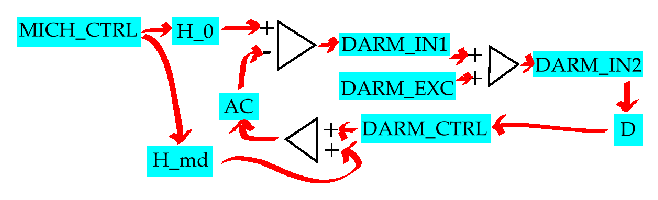
\includegraphics[height=120mm, width=160mm]{servo_loop.eps}
	\caption{Real-time servo loop diagram}
	\label{servo_loop_realtime}
	\end{center}
	\end{figure}

	\begin{figure}
	\begin{center}
	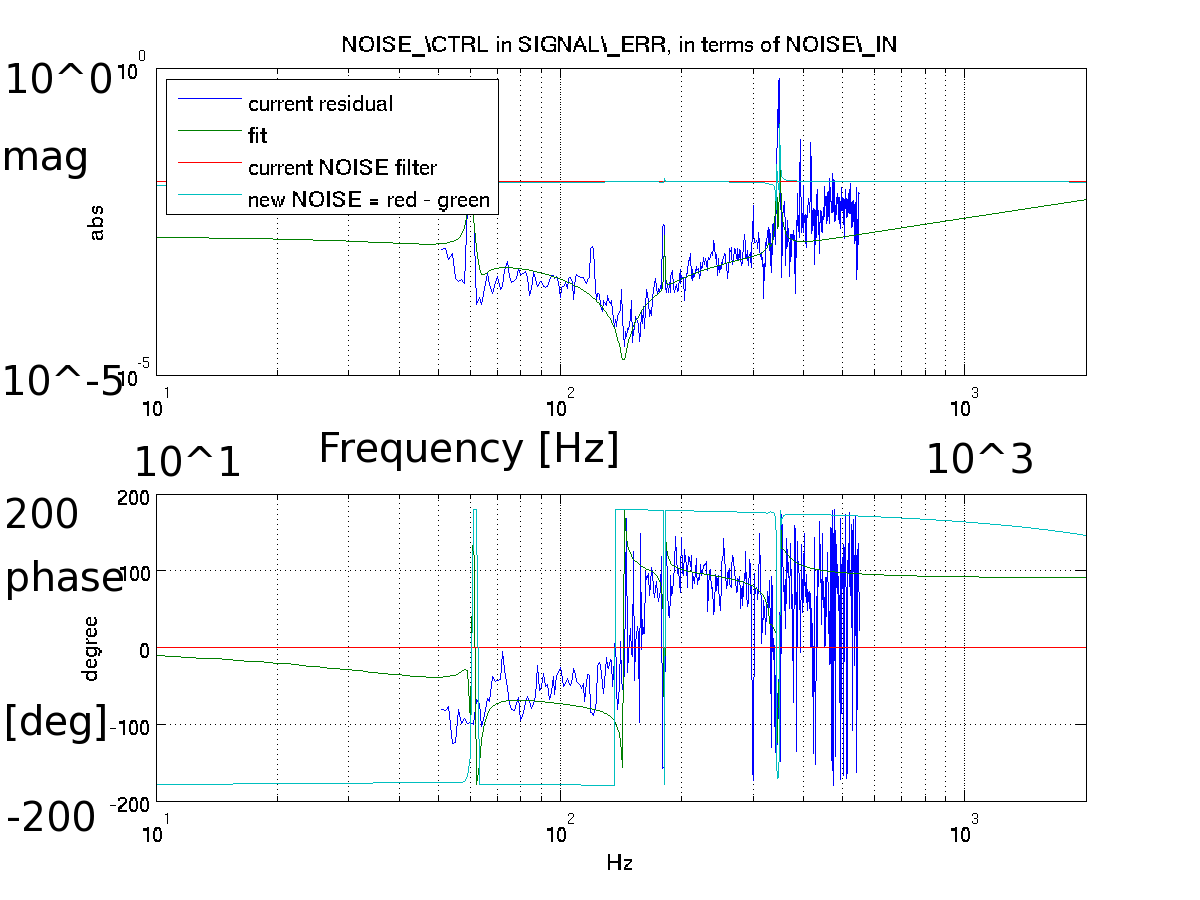
\includegraphics[height=120mm, width=160mm]{newNOISEfilter.eps}
	\caption{Real-time work on a LIGO noise filter}
	\label{newNOISEfilter}
	\end{center}
	\end{figure}

	\begin{figure}
	\begin{center}
	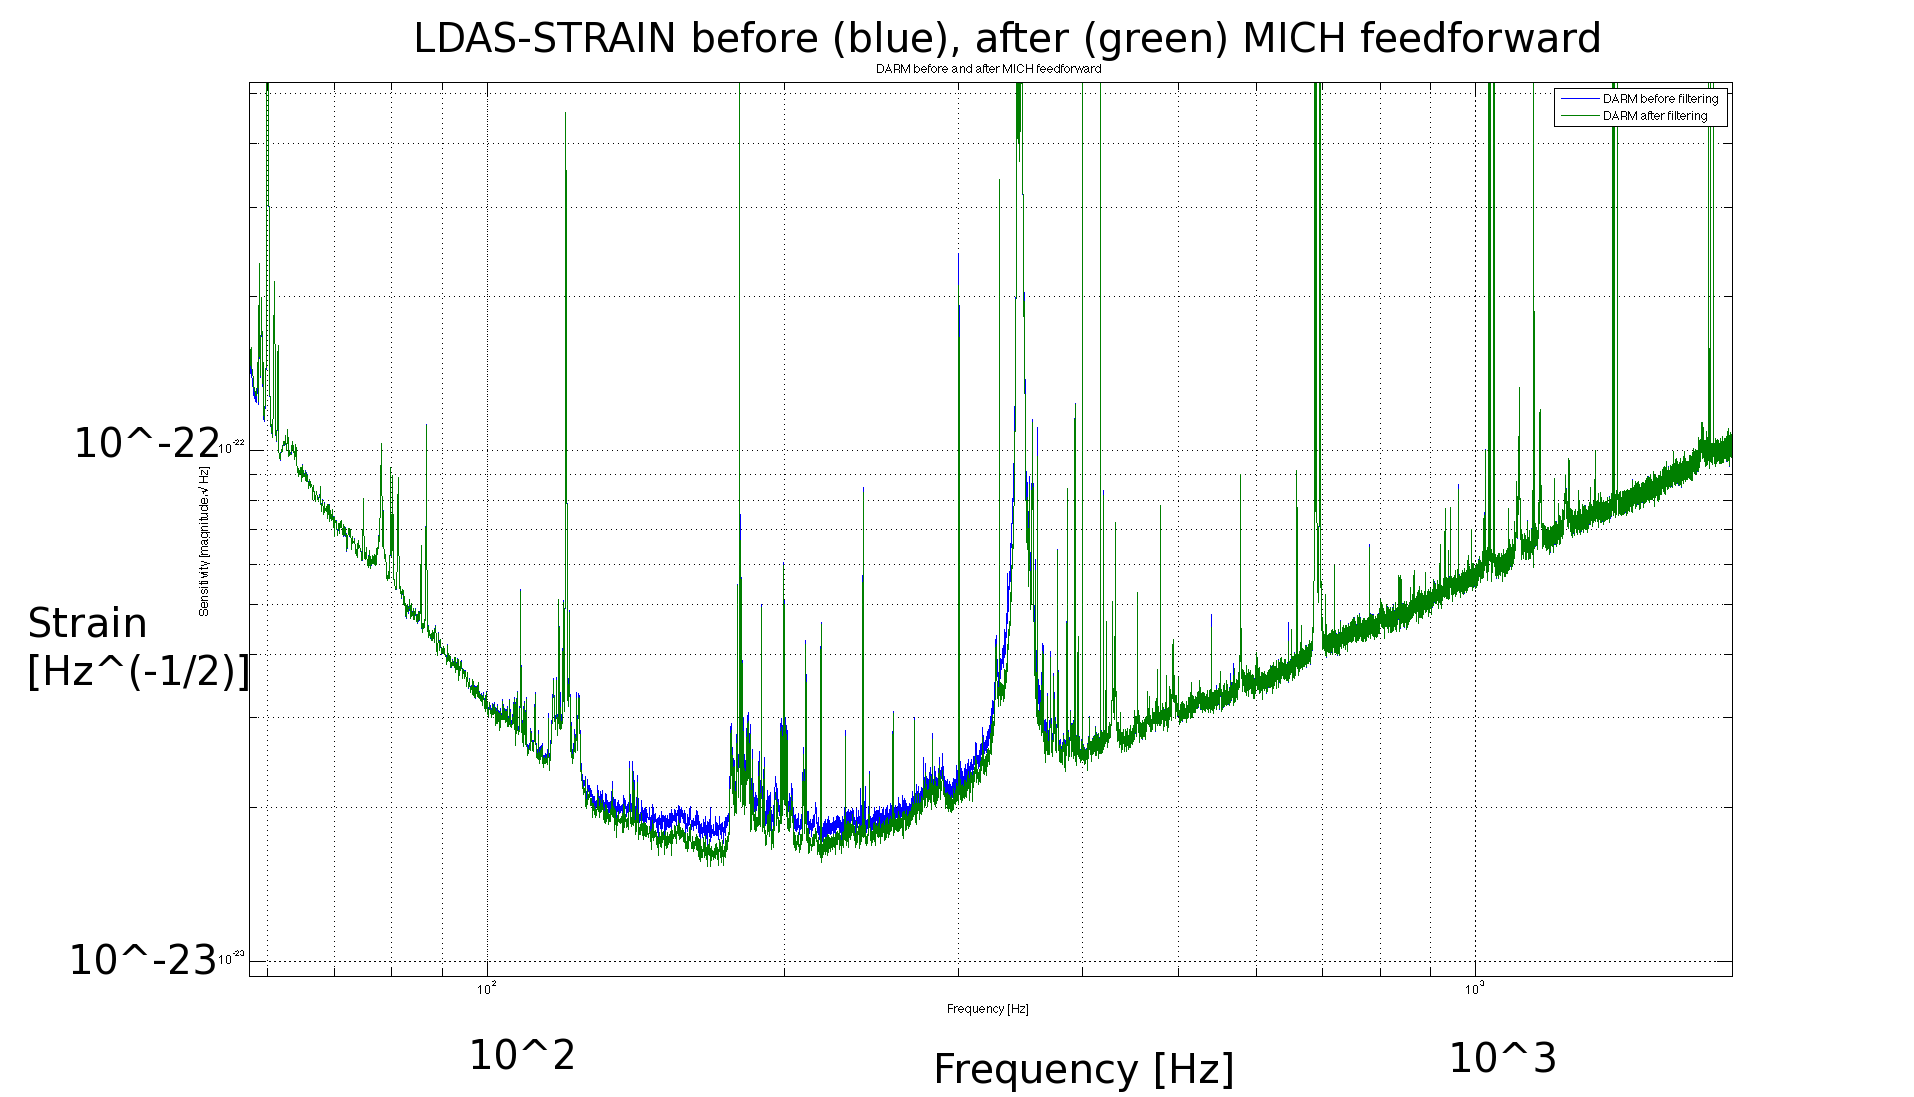
\includegraphics[height=120mm, width=160mm]{2011-03-08_filter-01.eps}
	\caption{Early work on post-facto noise filtering}
	\label{filter_early}
	\end{center}
	\end{figure}

                \paragraph{Phase camera}
                \label{phase_camera}

                    Future devices: overview of phase camera with Vladimir. Vladimir's thesis definitely talks about it~\cite{DergachevThesis}. We can discuss the fundamentals behind the need for angular stabilization and control from Nergis Mavalvala's thesis~\cite{MavalvalaThesis}, but we can refresh it with a modern reference from Kate Dooley's thesis~\cite{DooleyThesis}.


        \subsection{Advanced observatories and beyond}
        \label{advanced}
  
            Advanced LIGO and beyond -- squeezing and prospects?

        \subsection{Worldwide network}
        \label{worldwide}
 
            Allies: LIGO India, KAGRA, Advanced VIRGO, Einstein Telescope, LISA

    \section{Summary}
    \label{intro_summary}
 
        %Summary: strong motivation and instruments, need to find evidence of GW.    

Initial LIGO, during the science runs S6, would have been able to see the coalescence of two neutrons stars at about twenty Megaparsecs, out in the Virgo cluster of galaxies, from sixty-five million years ago, when dinosaurs still walked the Earth. 
In the first week of Advanced LIGO lock at Livingston, following Memorial Day 2014, Advanced LIGO had a temporal range extending only as far back as when early humans began their diaspora from Africa -- a terrestrial parallel to the expansion of the cosmos.
When completed, the Hanford and Livingston second-generation interferometers should see back ten times beyond what S6 could, six hundred and fiften million years, to before the Cambrian explosion of life.
Perhaps in the third or fourth generation of interferometers, our view of the gravitational sky may stretch back the age of the observable universe.
Even then, we will not have seen all that can be seen.
With the two long-range forces of the universe, electromagnetism and gravitational, giving two complimentary views of spacetime, we still must build great machines to explore the sights they show, we must understand what we are seeing, and we must propogate that understanding. 

This thesis is a prelude to those efforts, from the building of the quantum optical squeezer, and the feedforward regression and continuous waves binary search, to our public interferometer exhibitions.   
Feedforward regression provides a microcosm of the complexities of gravitational wave interferometry, so there we will begin.


            
%        --------------------
%
%	Here is a sample chapter file. The chapters of the thesis
%	should be saved to seperate files such as
%	\textit{chapter1.tex}. In the file \textit{thesis.tex} the
%	\textit{input} command then includes these chapters into the
%	thesis. Note that none of the chapter files need any headers.
%	This header for each of these files is contained in
%	\textit{thesis.tex}. The file \textit{thesis.tex} also
%	includes the numbers system for the sections, figures,
%	theorems lemmas etc...

%\section{Sample Section}
%\label{sample_section}
%
%	This is what a sample section looks like. Let's conclude this
%	section with a sample theorem statement and proof.
%
%	\begin{theorem}
%	\label{sample_theorem}
%	The are an infinite number of prime numbers
%	\end{theorem}
%
%	\emph{Proof:} On the contrary assume there are a finite number
%	of primes $P_1, P_2, ... P_n$. Consider $\mathcal{P} = P_1 P_2
%	\cdots P_n+1$. $\mathcal{P}$ is not divisible by any of the
%	primes in our finite set. (Contradiction) $\square$
  


% General relativity, history, mathematics
% Also include...
% Early phase camera work, explanation of LIGO and
% the summer of 2009 doing small projects, e.g. Omega scans
% and detector characterization with Rana, Mike and Keita
\chapter{Feedforward: Auxiliary MICH-PRC Subtraction}
\label{chap2}
        
        \section{Cosmic sources of gravitational waves}
        \label{cosmic_sources}
      
        %   --- Cosmic origins believed to generate GW. (note: should sprinkle citations as needed, not just where it says "cite") ---

		Gravity's power induces ripples in space. 
Pulsar 1913+16, discovered by Hulse and Taylor in radio waves, not only followed a pattern of orbital decay consistent with radiative energy loss to gravitational radiation -- it continued to do so~\cite{WeisbergTaylor2004,Weisberg2010}, seen in Figure~\ref{Hulse-Taylor_binary}, after the 1993 physics Nobel Prize. 
This year, there has been much debate as to whether or not the BICEP2~\cite{BICEP2014} and Planck~\cite{Planck2014} probes of the cosmic microwave background have seen evidence of $B$-mode polarizations that would indicate primordial gravitational fluctuations due to inflation.
Eventual identification of the polarization is expected by many, regardless~\cite{Baumann2009}. 
We still may ask whether any gravitational waves will be directly detectable on Earth. 
We may ask whether they appear in detectors in a way consistent with General Relativity. 
The basic fact of their emission, however, appears settled.

	\begin{figure}
	\begin{center}
	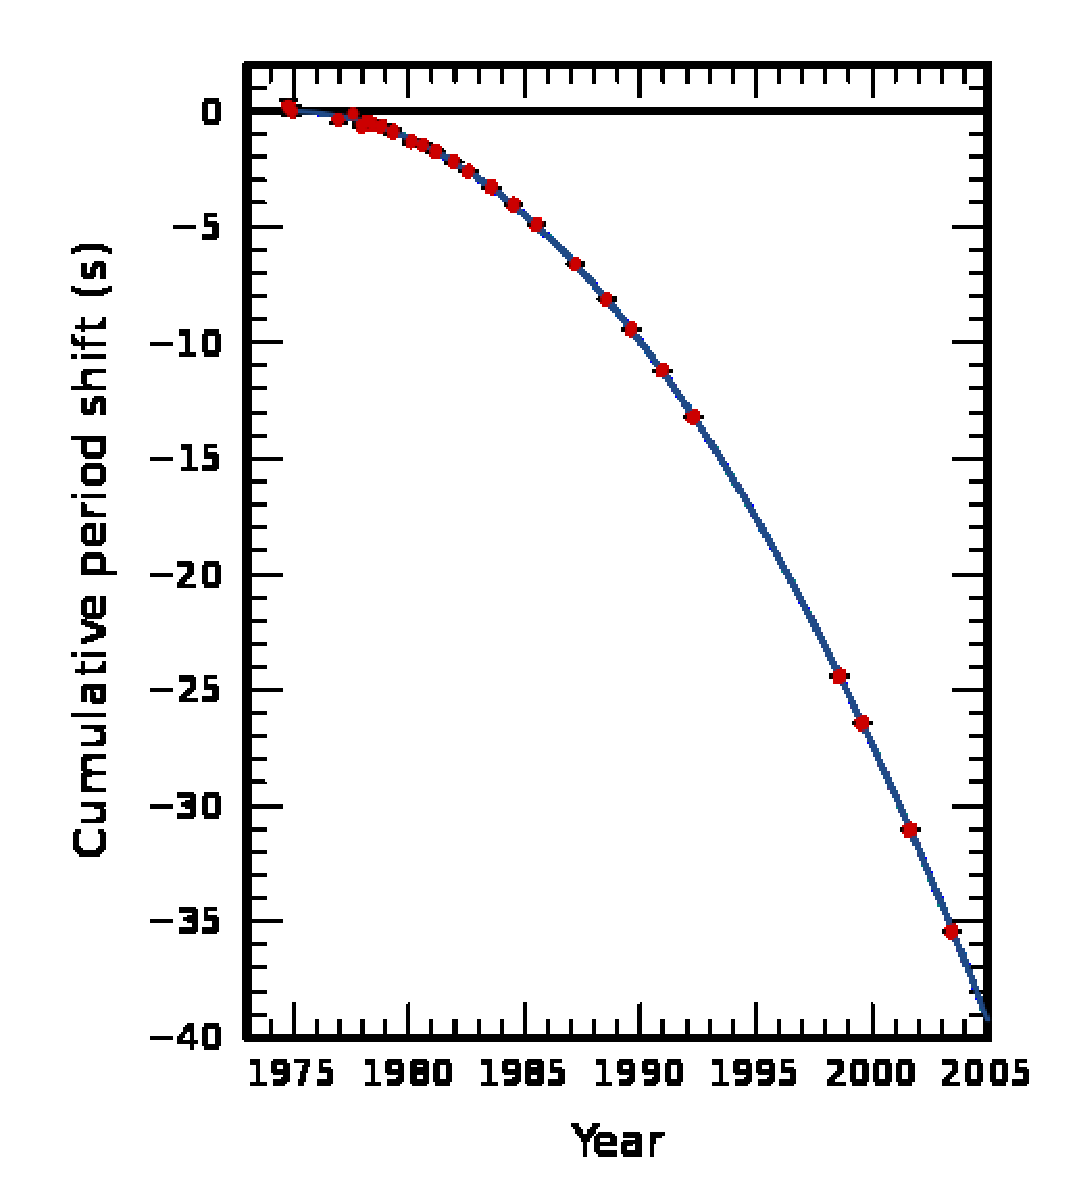
\includegraphics[height=111mm, width=148mm]{500px-PSR_B1913+16_period_shift_graph.eps}
	\caption{The Hulse-Taylor binary PSR 1913+16, orbital period change over time consistent with emission of gravitational radiation from its system~\cite{Weisberg2010}. Gravitational waves emission depletes orbital energy, causing the binary stars to slowly inspiral into closer orbits. Shrinking pulsar radius $R$ leads to the shorter period $T$ -- Kepler's third law, $T \propto R^{3/2}$ (first stated in \textit{Harmonices Mundi}~\cite{Hawking2002}). Timing error can be ruled out, because the orbital decay is not linear.}
	\label{Hulse-Taylor_binary}
	\end{center}
	\end{figure}

Before delving into general relativitic emission, let us consider the astrophysical sources expected to emit gravitational waves. 
Physics prompts our search, but astronomy richens it.
When gravitational waves are heard by the interferometers, we will be hearing the songs of dead stars, rippling through the fabric of spacetime.  
Gravitational waves (henceforth also abbreviated GW) searches presently focus on four distinct types of cosmic sources.
This categorization of sources was first presented no later than the 1983 LIGO Blue Book proposal and has since guided research focus~\cite{CollinsGravityShadow,Schutz1989}. 
The quadripartite division:
\begin{itemize}
\item Burst (rarely, `supernova')
\item Compact binary coalescence (or `inspiral')
\item Continuous wave (or `pulsar')
\item Stochastic
\end{itemize}

This thesis concentrates on continuous waves (CWs) -- sine waves. 
CWs are most likely to emanate from neutron stars. 
Neutron star CWs can be modulated by orbital motion, spun-up from accretion or spun-down from radiated energy. 
Given a sufficiently large ellipticity, on the order of $\epsilon \approx 10^{-7}$~\cite{Owen2005} or smaller for a neutron star rotating on the order of 1 kHz, a crust deformation (alternatively an $r$-mode~\cite{Owen1998,Owen2010}) would radiate sufficient gravitational radiation to be a plausibly detectable source. 
In an isolated neutron star, GW radiation would rapidly deplete rotational energy~\cite{Owen1998}.
Binary systems, where the neutron star could be recycled and spun-up by a partner~\cite{PapaloizouPringle1978,Wagoner1984}, would last longer in contrast.
Scorpius X-1 offers a canonical case~\cite{AbbottScoX12007}, although TwoSpect (a search for neutron stars in binary systems, detailed in this thesis) anticipates an abundance of other low-mass X-ray binary (LMXB) systems of interest. 
Given the paucity of insight on the interiors of collapsed stellar remnants, direct detection of GWs from neutron stars would prove informative~\cite{Lindblom1995}. 
Just as we might infer details from neutron star binary coalescences favoring one equation of state~\cite{Lattimer2007,Read2009}, we might also extract parameters from continuous waves suggesting the existence of quark stars or gravitars~\cite{Owen2005}, and will have an unparalleled peek into the interior of the densest stable three-dimensional objects in the universe. 
Their simple waveforms might even facilitate the calibration of other types of GW data, whereas binary mergers should sound like standard sirens to compare against electromagnetic and neutrino observations~\cite{Punturo2010}
(see next paragraph).
CWs are conceptually elegant and astronomically enticing.
Yet other sources of GWs have a comparable pull on our attention. 

Inspirals or compact binary coalescences occur when two stellar remnants draw nearer in their orbits, radiating gravitational radiation and finally merging in a titanic release of energy. 
While sometimes invisible -- except as short-hard gamma ray bursts (GRBs) -- these events compete with supernovae as the most explosive in the modern universe. 
Were GW observatories to see their waveforms, they could be compared with those predicted through post-Newtonian approximation and numerical relativity. 
As GW amplitude should diminish inversely with distance, we would then have standard candles or \textit{standard sirens} by which to calibrate and measure the universe. 
Advanced LIGO~\cite{aLIGOrefDesign,aLIGOsysDesign} may prove sensitive to neutron star-neutron star and stellar mass black hole-neutron star mergers, and, if low-frequency sensitivity is sufficient and the sources exist, to intermediate-mass black holes. 
Proposed space-based observatories such as the long-suffering Laser Interferometer Space Antenna (LISA) and ensuing DeciHertz Gravitational-wave Observatory (DECIGO) \& Big Bang Observer (BBO) could detect supermassive black hole mergers. If launched, they would see a low-frequency noise floor due not to seismic vibration, as in LIGO, but to white dwarf binaries throughout the galaxy. 
Since the waveforms are well-predicted, we could even investigate deviations from General Relativity, perhaps seeing new physics in the ringdown of highly massive black holes.

Physical insight could also come from burst searches. 
Bursts searches share with inspiral searches the property of looking for a single transient event, as opposed to a source spread over long duration. 
Analytical programs for bursts can sometimes be applied to inspiral or detector characterization tasks as well; rare noise events are a limit on their astronomical sensitivity.
Yet the immediate focus lies with supernovae~\cite{Chandrasekhar1969,Ott2009} and perhaps gamma-ray bursts. 
Because the waveform is unknown, burst searches rely significantly more on the coincidence between multiple detectors to distinguish signal from noise. 
Just as with neutrino observations of supernova 1987A, the burst program would hope for a fortuitously nearby cataclysm to be seen simultaneously -- or nearly so, the time of flight indicating a direction -- in a global gravitational-wave detector network. 
Due to the versatility of this method, some researchers have proposed looking for longitudinal polarization in addition to plus and cross orthogonal polarization (possible in non-general relativistic terms; see Section~\ref{history_GR}). 
Any detection would be quite exciting for probing still mysterious systems with electromagnetic and neutrino measurements, and it would help, in conjunction with multi-messenger coordinated searches with those observatories, to ascertain at precisely what speed gravity travels through space-time and to what extent it is attenuated or altered.

The background of space-time itself may hide GW signatures. 
Searches for the stochastic GW background look not for single events but for persistent phenomena buried in many months of correlated signals between networks of detectors. 
In doing so, they hope in particular to see the earliest turbulence of the universe.
 Long before the cosmic electromagnetic background was emitted 380000 years after the Big Bang -- now redshifted into microwaves -- GWs were travelling unimpeded. 
While the opacity of the infant cosmos conflates electromagnetic signals from different times and places, the transparency of the universe to gravity means that we might see the inflationary epoch. 
Unfortunately, this signal is thought to be far below the sensitivity of existing detectors in the LIGO band. 
While LIGO did set a new upper limit on the energy density of GWs, measured as a fraction, $\Omega_{gw}$ of the critical closure density of the universe~\cite{LIGOStochasticNature2009}, the inflationary background at LIGO frequencies is predicted to be about ten orders of magnitude lower. 
Alternative theories, such as ekpyrotic/cyclic universes or an axionic inflaton, make other predictions; an anomalously high stochastic background could thus prove cosmologically significant.

All GW searches strive to open up new directions in astronomy. 
While the most exciting possibility is that we will see the unexpected, we think that our present algorithms will permit serendipity. 
Continuous wave and inspiral methods both search against waveform templates; burst and stochastic have no template and rely on correlation and coincidence. 
Continuous wave and stochastic searches analyze weeks, months, even years of data in search of persistent features; inspiral and burst searches look for transient events. 
In the abstract dimensions of search groups, we are complete. 
Our attention is narrow now -- in the focus on audio frequencies of tens to a few thousand Hertz at present -- narrowness that will in time be broadened by CMB polarization, pulsar-timing and space-based interferometry for low frequencies and possibly by atom interferometry~\cite{Dimopoulos2009} around 1 to 10 Hz. 
To appreciate our choice of focus in these nascent days of the field, we must turn back a century to understand its origins in Einstein's mathematics.

        \subsection{History from General Relativity}
        \label{history_GR}

            %Historical brief of Einstein.
        Einstein's theory unified a sequence of historical insights. 
Since 1676, when Roemer used the moons of Jupiter to measure the finite speed of light, just before Newton's 1687 \textit{Principia Mathematica}~\cite{Hawking2002}, the question of gravity's propagation beckoned. 
Bringing together the work of Minkowski and Poincar\'{e}, the 1905 special theory of relativity highlighted the naturalness of the speed of light, but only in 1915, with the presentation of the Einstein field equations of General Relativity, based in Riemannian geometry, did a means to an answer emerge. 
In 1916, Einstein predicted GWs. 
At last, gravity had a theoretical speed: the same as for electromagnetism, that of light in the vacuum, $c$.
In the linear approximation to the nonlinear theory of General Relativity (henceforth GR), the waves were mathematically similar to the waves of electromagnetism, as will be shown in Section~\ref{general_relativity}.
GR offers a consistent explanation for how changes in the distribution of matter change gravitational fields.
Yet the detectability of the waves, even in principle, would remain an open question for another half century. 
Uncertainty in whether fluctuations within spacetime could be detectable with instruments themselves changed by the same fluctuations dominated the debate. % Insert add'l ref
Thought notions, \textit{Gedankenexperiment}, such as beads-on-rods led to consensus that GWs carried and could deposit physical energy and thus be detected. 
Consult Misner, Thorne, and Wheeler's \textit{Gravitation}~\cite{MisnerThorneWheeler} and Sean Carroll's lectures notes~\cite{Carroll1997}, as well as other history books of the field for an account of the controversy.
Saulson~\cite{Saulson1997} explicates both why gravitational waves should be detectable in theory and why travel time is superior to wavelength in understanding GW interferometry.
See \textit{Gravity's Shadow}~\cite{CollinsGravityShadow} for sociological perspective, and 
\textit{Gravity's Ghost}~\cite{CollinsGravityGhost} for insight into the detection criteria that have since evolved\footnote{See also a recent review by Riles~\cite{Riles2013}.}.

Discussions of GWs frequently begin with derivations of the wave equations from Einstein's field equations. 
General relativity, however, is not the only theory to predict GWs: waves are a natural consequence of a class of similar theories, which make a range of testable predictions (such as number of polarization modes, from two to six, and possibly speeds different from $c$)~\cite{Will1993}. 
Waves should thus be expected even if some small variation from Einstein's theory is discovered, pointing a way perhaps toward a quantum theory of gravity~\cite{Sathyaprakash2009}. 
%As the field progresses toward first detection and beyond to astronomy, the astrophysical targets of our searches should take precedence.

Before deriving the answer to the detectability question from the field equations, a contrast with the situation in other fields of astronomy is in order.

 
        \subsection{Contrast with electromagnetic and particle astronomy}
        \label{contrast_astro}

        With astronomy, detection came first, then theory.
Visible light astronomy began with the earliest humans.
Records of the star Sirius are known from Egyptian astronomers, the planet Venus from Babylonians, sunspots from the Chinese, and eclipses from the Greeks. 
Thus the telescope, though revolutionary, was not unimaginable.

Infrared radiation, as first seen by William Herschel, was just beyond the visible red light of a prism.
As the wave nature of light came to be understood, culminating in Maxwell's equations, the existence of invisible electromagnetic radiation was put on sound theoretical footing.
The only remaining questions pertained to whether this radiation would prove astronomically interesting, especially in the extreme low- (radio) and high- (X- and $\gamma$-ray) frequencies found at the end of the 19th Century.
Fortuitiously, unlike with GWs today, these novel bands of electromagnetic spectrum could be easily generated and detected by scientists in small laboratories, as with Marconi and Marie \& Pierre Curie.
Within half a century, radio telescopy began with Karl Jansky~\cite{Shklovsky1960}, with Grote Reber soon observing the Milky Way~\cite{Gurzadyan1956}.
By the early 21st Century, radio astronomy ranged from common rooftop designs~\cite{SRT} (nonetheless sensitive enough to infer the galactic rotation curve in the hydrogen line~\cite{MeadorsThesis2008}) to planetary-scale very long baseline interferometry and plans for a Square Kilometer Array.
Electromagnetic, or photon, astronomy has the advantage of calibration with familiar sources.

%            Contrast with electromagnetism, compare with radio/X-ray/et cetera astro. 

%Can make analogy to radio waves and make note of the ease with which one can operate a small radio telescope, as I did in my thesis~\cite{MeadorsThesis2008}, compared the the difficulty of GW detection. 

Other particles besides the photon began to play a role in 20th Century astronomy.
Muons from space were detected long ago, as in C.D. Anderson's 1949 paper on what was then called the mesotron~\cite{CDAnderson}. 
Solar neutrinos were, after much difficulty, seen by Ray Davis~\cite{NeutrinoReview}, and neutrino astronomy was a well established field by the turn of the millenium, following the detection of Supernova 1987A in the Large Magellenic Cloud. 
New types of neutrino detectors\footnote{For example, time-projection chambers using electron bubbles in cryogenic noble gas such as helium or neon, the subject of some prototype construction and simulation research by the author~\cite{EBubble2005,MeadorsNevis2006}.} could yield additional information and better sensitivity.
As with electromagnetic waves, humans can generate a measurable neutrino flux. 
Since the Savannah River nuclear reactor experiments, the experimental detectability of neutrinos has been settled.
Solar neutrino observations spurred a deeper understanding of neutrino oscillation to coincide with theory~\cite{NeutrinosSolarTheoretical}; now, astrophysics with neutrino observatories is becoming mature.
Nuclear fusion in the Sun has been well-established, and arrays such as Antares~\cite{Antares2013} and IceCube~\cite{Aartsen2014} will move the field outwards toward cosmic sources.


 GWs from the PSR 1913+16 system itself~\cite{WeisbergTaylor2004} are too low in frequency to be seen with existing interferometers, but they confirm that the phenomenon is real.
Although no terrestrial sources of GWs can be feasibly generated, calibration~\cite{AbadieCalibration2010} of interferometers is nonetheless accurate to a few percent.
Direct detection of GWs would let us infer the true strength of astrophysical gravitational radiation and compare that power with theory. 
Surprising new insights are probable in any new field, not unlike the discovery of neutrino oscillation in the solar spectrum or the anomalous galactic rotation curve due to dark matter.

Yet how can gravity be seen?
GWs are conceptually simple, with mathematics illustrated by electrodynamic analogy in the Appendix.
A short derivation follows.

    %End section by very rapidly deriving wave equation of electricity and magnetism, to lead by example for how we go about GR.
    %Note that all physics in min(action),
    %introduce metric as inner product
    %generally, coordinate transform good



    \section{General relativity}
    \label{general_relativity}

        Einstein's theory of General Relativity (hence GR) describes gravitation as curvature. 
Gravity is a pseudoforce, unlike Newton's force $\textbf{F} = -G_C M_1 M_2 r^{-2} \hat{\textbf{r}}$ for two bodies of masses $M_1$ and $M_2$ separated by a vector distance $\textbf{r}$ in a universe with a gravitational constant $G_C$ (henceforth, units are set where $G_C \equiv 1$).
 Einstein posits that objects always follow an extremized path, $\delta s = 0$ for arclength $s$  -- a geodesic worldline -- when the curvature of spacetime is considered. 

The curvature of spacetime is described by the Riemann tensor, $R^\mu_{\nu\rho\sigma}$, which physically is required to be a solution to the Einstein field equations. 
Section~\ref{field_equations} clarifies the connection between these field equations and the Ricci scalar curvature $R$, a trace of the Riemann tensor, whence they can be derived. 
This Riemann tensor is constructed from the Christoffel connection, $\Gamma^\mu_{\rho\sigma}$, which in turn can be expressed in terms of the metric, $g_{\mu \nu}$.
It is the metric that measures distance across spacetime: $ds^2 = g_{\mu\nu} dx^\mu dx^\nu$.
Hence the psuedoforce of gravity is, in GR, curvature distortions (arising from matter) that change the distance along worldlines and thus affect trajectories.

For more mathematical detail, please see the Appendix.
 Carroll and \textit{Gravitation} are useful references~\cite{Carroll1997,MisnerThorneWheeler}, consulting other sources for the Einstein-Hilbert/Palatini action~\cite{FarrThesis}.

%            Introduce the metric $g$ here, but reinforce that it is not essential.
%Intro to GR -- right motivation is least action Ricci tensor, implying field equation and phase/time-of-flight implying interferometry.

        \subsection{Symmetry and action principles}
        \label{principles}

Einstein's geodesic equation is a replacement for not only Newton's law of gravitation but also for the Laws of Motion.
An object's acceleration is described in terms of its proper time and the Christoffel connection.
The supposition that objects follow a geodesic path follows from Fermat's principle of least time, which also inspired the least action principle, $\delta \mathcal{S} = 0$.
In turn, interferometry is best understood in terms of least-time phase or \textit{time-of-flight}.

Gauge symmetries and the associated conservation laws of Noether's theorem have been critical to the development of quantum field theory. 
Whereas electromagnetism arises from $U(1)$ unitary Lie group gauge symmetries, the electroweak force from $SU(2) \times U(1)$, and quantum chromodynamics from $SU(3)$, GR arises from $GL(4, \mathbb{R})$ general linear Lie group symmetries. 
These symmetries are \textit{diffeomorphism invariances} with respect to Lorentz boosts and translations, meaning we can \textit{pullback} vector fields, such as the other forces, through a coordinate change without changing their physics.
Ergo the conservation laws that emerge from GR are the familiar ones from mechanics -- stress-energy, momentum, and so on, with subtleties (particular for non-static universes).

%           Like electricity and magnetism, GR is the product of symmetry, action. 


        \subsection{Derivation of field equations}
        \label{field_equations}

            A common approach to GW derivations is linearized GR~\cite{FlanaganHughes2005}.
            Linearization proceeds~\cite{AdhikariThesis} from the metric $g_{\mu\nu}$ approximation as the sum of a Minkowski (flat spacetime) component, $\eta_{\mu\nu}$, plus a perturbation $h$, where $|h_{\mu\nu}| \ll |\eta_{\mu\nu}|$, so $|h_{\mu\nu}| \ll 1$:

\begin{equation}
g_{\mu \nu} \approx \eta_{\mu \nu} + h_{\mu \nu},
\label{perturbation_eq}
\end{equation}

\noindent the weak-field approximation, leading to a wave equation, notated by a d'Alembertian $\Box = \partial_\mu \partial^\mu$,

\begin{equation}
-\frac{1}{2} \Box \left(h_{\mu \nu} - \frac{1}{2} \eta_{\mu \nu} h_{\lambda}^{\lambda} \right) = \frac{8 \pi G_C}{c^4} T_{\mu \nu}.
\label{Ballmer_wave_eq}
\end{equation}

The right-hand side indicates that GWs are sourced by the stress-energy tensor, $T_{\mu\nu}$, which subsumes the electromagnetic stress-energy, pressure, and density terms. 
For gravitational sources of astrophysical interest, the majority of sourcing comes from matter density -- since mass-energy is conserved, monopolar radiation is forbidden (formally, by the Birkhoff theorem), and conservation of linear and angular momentum forbids the dipole terms. 
GWs are thus sourced by quadrupoles $I_{ij}$ and higher only, although the higher-order terms are generally smaller and neglected. 
The wave does carry energy density $\rho_{gw}$ and power $P$~\cite{BallmerThesis}:

\begin{eqnarray}
\rho_{\textup{gw}} &=& \frac{c^2}{16 \pi G_C} \left\langle |h_{+,0}|^2 + |h_{\times,0}|^2 \right\rangle,\\
P &=& \frac{G_C}{5c^5}\left\langle \left( \partial_t^3 I_{ij}\right)^2  \right\rangle \approx 5.5\times 10^{-54} W^{-1} \left\langle \left( \partial_t^3 I_{ij}\right)^2  \right\rangle.
\label{energy-and-power_eq}
\end{eqnarray}

Equations~\ref{perturbation_eq}-\ref{energy-and-power_eq} represent the testable predictions of GR about GWs. 
GR itself is found by finding the field equations from the action~\cite{FarrThesis}, optimizing (extremizing) the integral of curvature: the Ricci scalar $R$.
Here $|g|$ indicates the determinant of $g$. Add two terms to $R$: a hypothetical constant, $\Lambda$ (termed the cosmological constant), and the matter Lagrangian density $\mathcal{L}_M$. The sum generates the Einstein-Hilbert action $\mathcal{S}$:

\begin{equation}
\mathcal{S} = \int \left( \frac{1}{8\pi}\left(R - 2\Lambda\right) + \mathcal{L}_M \right) \sqrt{-|g|}d^4 x,
\end{equation}

Extremizing $\delta \mathcal{S} = 0$ involves expanding $R = R^\mu_\mu$, where $R_{\mu\nu} = R^\lambda_{\mu\lambda\nu}$, the Ricci tensor. 
In turn, the Ricci tensor is contracted from the Riemann tensor, $R^\mu_{\nu\rho\sigma}$ (the curvature tensor, equivalently the 2-form $\textsf{R}^\mu_\nu$). Maurer-Cartan structure equations show how the Riemann tensor is an operator, the sum of a `differential' plus connection $\omega$, applied to the connection $\omega$ itself,

\begin{eqnarray}
\textsf{R}^\mu_\nu &=& d\omega^\mu_\nu + \omega^\mu_\rho \wedge \omega^\rho_\nu, \\
\omega^{\rho'}_{\mu\sigma'} &=& e^{\alpha'}_{\nu} e^{\lambda}_{\beta'} \Gamma^{\nu}_{\mu\lambda} - e^{\lambda}_{\beta'} \partial_{\mu} e^{\alpha'}_{\lambda},\\
\Gamma^\sigma_{\mu\nu} &=& \frac{1}{2} g^{\sigma\rho} \left( g_{\nu \rho, \mu} + g_{\rho \mu, \nu} - g_{\mu\nu,\rho} \right). 
\end{eqnarray}

\noindent where the last equation defines the \textit{Christoffel} connection. Just as metric induces distance on the spacetime Riemannian manifold, and the connection corrects geodesic paths, so the curvature tensor accounts for geodesic deviation between paths.

Substituting into the action, we obtain~\cite{Carroll1997} the \textit{Einstein field equations} by varying over the metric $g_{\mu\nu}$, we make use of the fact that $\delta R = (g^{\mu\nu} \delta R_{\mu\nu} + R_{\mu\nu} \delta g^{\mu\nu})$ (the first term of which vanishes due to Stokes' theorem).
The equations are often simplified using the Einstein tensor, $G_{\mu\nu} \equiv R_{\mu\nu} - (1/2)R g_{\mu\nu}$:

\begin{eqnarray}
\delta \mathcal{S} &=& \int d^4 x \left( \frac{\delta R \sqrt{-|g|} + (R-2\Lambda)\delta \sqrt{-|g|}}{8\pi}+ \delta (\sqrt{-|g|}\mathcal{L}_M)\right), \\
 &=& \int d^4 x \sqrt{-|g|}\left( \frac{\delta g^{\mu\nu}}{8\pi} \left[ G_{\mu\nu} + \Lambda g_{\mu\nu} \right]
 + \frac{\delta g^{\mu \nu}}{\sqrt{-|g|}} \frac{\delta (\sqrt{-|g|}\mathcal{L}_M)}{\delta g_{\mu\nu}} \right).
\end{eqnarray}

\noindent Since the integral must vanish everywhere,
\begin{eqnarray}
\frac{1}{8\pi} \left[G_{\mu\nu} + \Lambda g_{\mu\nu} \right] = -\frac{1}{\sqrt{-|g|}}\frac{\delta (\sqrt{-|g|}\mathcal{L}_M)}{\delta g_{\mu\nu}}.
\end{eqnarray}

\noindent The field equations are sourced by the right-hand side, identified (e.g., by comparison with Newtonian gravity) with the stress-energy tensor, $T_{\mu\nu}$:

\begin{equation}
G_{\mu\nu} + \Lambda g_{\mu\nu} = 8 \pi T_{\mu\nu}.
\label{great_einstein_field_equations}
\end{equation}

Einstein's concern was the different nature of the source term.
Much of the effort toward unifying GR with the other forces can be understood as trying to fuse the matter Lagrangian with the Ricci scalar in an intuitive way.

The linearized wave derivation in transverse-traceless gauge is standard in GWs. 
Radiation in the non-linear near-field is explored by numerical relativistic studies~\cite{FarrThesis}.
Equation~\ref{great_einstein_field_equations}, however, also allows derivations using the curvature.
This derivation makes it easier to compare interferometer observations (of length scale $L$ much smaller than GW wavelength $\lambda$) with less-linear spacetimes or where $L$ is comparable to $\lambda$.
In vacuum, the Riemann tensor satisfies a non-linear covariant wave equation in any gauge~\cite{KoopFinn2014}, $0 = R_{\mu \nu \rho \sigma; \lambda}^{\textup{        } \lambda} + S_{\mu \nu \rho \sigma}$, where the $S_{\mu \nu \rho \sigma}$ is quadratic in the Riemann tensor and therefore negligible.
The first-order perturbative response of the Riemann tensor in Minkowski space of an observer at rest, in conventional transverse-traceless gauge (see below), to a metric perturbation $\bar{h}_{\mu\nu}$ is then,

\begin{equation}
R_{0\mu0\nu} = -\frac{1}{2} \bar{h}_{\mu\nu,00}.
\label{Finn_wave_eq}
\end{equation}

%\noindent Seen another way~\cite{KoopFinn2014}, a perturbation $h_{\mu\nu}$ leads to a first order perturbation in the Riemann tensor:
%\begin{eqnarray}
%R^{(1)}_{\mu\nu\rho\sigma}= h_{\lambda\sigma} R_{\mu\nu\rho}^{(0)\lambda} - \frac{1}{2}\left( \right)
%\end{eqnarray}

\noindent Obtaining this first-order response recovers the common formalism~\cite{BallmerThesis}, where a metric perturbation is substituted into Equation~\ref{great_einstein_field_equations} to yield,

\begin{equation}
G_{\mu\nu} = -\frac{1}{2}\left(h_{\mu\nu,\lambda}^{\textup{       }\lambda} - h^\lambda_{\mu,\lambda\nu} -
h^\lambda_{\nu,\lambda\mu} + \eta_{\mu\nu}(h^{\lambda\sigma})_{,\lambda\sigma} - \eta_{\mu\nu}(h_\sigma^\sigma)_{,\lambda\lambda} - (h_\sigma^\sigma)_{,\mu\nu}  \right),
\end{equation}

\noindent simplified by switching coordinates to a traceless gauge, defined by $\bar{h}_{\mu\nu}\equiv h_{\mu\nu} - (1/2)\eta_{\mu\nu}h_\lambda^\lambda$, that obeys the harmonic (transverse) condition, $\bar{h}_{\mu\nu} = 0$, into

\begin{equation}
G_{\mu\nu} = -\frac{1}{2} \bar{h}_{\mu\nu,00} = 8 \pi T_{\mu\nu}.
\label{General_Ballmer_wave_eq}
\end{equation}

\noindent Equation~\ref{General_Ballmer_wave_eq} is the origin of Equation~\ref{Ballmer_wave_eq} and also corresponds to Equation~\ref{Finn_wave_eq}. 
Moreover, outside a source, we can impose the transverse-traceless gauge, which verifies that in vacuum $\bar{h}_{\mu\nu} = h_{\mu\nu}$.
The curvature wave equation is what is fundamental.

However described, the wave, parametrized by path $x^\mu (\lambda)$ follows the same geodesic equation as light, where the covariant derivative by $\mu$ of $V^\nu$ is defined by $\nabla_\mu V^\nu = (\partial_\mu V^\nu + \Gamma^\nu_{\mu\lambda} V^\nu)$ and along a path~\cite{Carroll1997} by $D_\lambda = dx^\mu_\lambda \nabla_\mu$,

\begin{equation}
D_\lambda \partial_\lambda x^\mu = 0
\end{equation}

In GR, the six possible independent components of the waveform reduce to just two $h_+$ \& $h_\times$ terms, although other theories of gravity predict additional polarizations.
These plus $h_+$ and cross $h_\times$ polarizations make the metric waveform along the $z$-axis ($k_\mu = \textup{diag}(1,0,0,\omega)$, initial phase $\phi_0$) in transverse-traceless gauge:

\begin{equation}
h_{\mu\nu} =
\left[
\begin{array}{cccc}
0 & 0 & 0 & 0\\
0 & -h_+ & h_\times & 0 \\
0 & h_\times & h_+ & 0\\
0 & 0 & 0 & 0
\end{array} \right] \Re \left(e^{\sqrt{-1} (k_\mu x^\mu + \phi_0)} \right).
\label{GW-matrix-eq}
\end{equation}

\noindent Tensor polarization corresponds to the prediction of hypothetical gravitons being spin-two particles, analogous to the spin-one photon with a vector-polarized electromagnetic field.
GWs in GR travel at the same speed of light as electromagnetic waves, for which experimental data~\cite{CODATA} has matched theory~\cite{GriffithsE} so well that $c$ is now embedded into our system of units.
Unlike light, which has complex interactions with interstellar media~\cite{Caldwell1981,McKee1977}, GWs should pass almost unimpeded through the stars. 
While the transverse-traceless equation describes the (near-)vacuum, far-field GWs we seek to detect, the source term in Equation~\ref{General_Ballmer_wave_eq} must be understood to justify our expectation of astrophysical sources.


        \subsection{Radiation from quadrupoles}
        \label{radiation}

Section~\ref{field_equations} notes that monopole and dipole sources are forbidden by conservation of mass-energy and momentum. This leaves us to derive radiation from quadrupolar sources in the stress-energy tensor.
Starting from the field equations, a Green's function $G$ (impulse response) lets us invert the linear differential operator $\Box$ by solving for a point, Dirac delta source $\delta$~\cite{Carroll1997}.
As with electromagnetism, the retarded Green's function from a source at $y^\sigma$ to an observer at $x^\sigma$ is given (where the Heaviside step-function is $\theta$) by, 

\begin{equation}
G(x^\sigma - y^\sigma) = - \frac{1}{4\pi |x^i - y^i|}\delta \left(|x^i - y^i| - (x^0 - y^0)\right)\theta(x^0 - y^0).
\end{equation}

\noindent Hence the source integral is (n.b., $\sqrt{-|g|} = 1$ in flat space),

\begin{eqnarray}
\bar{h}_{\mu\nu} &=& -16\pi \int d^4 x \sqrt{-|g|} G(x^\sigma - y^\sigma) T_{\mu\nu}(y^\sigma),
\\
 &=& 4 \int \frac{d^3 x}{|x^i - y^i|} T_{\mu\nu} \left(t - |x^i - y^i|, y^i \right).
\end{eqnarray}

\noindent Note that the latter equation is integrated over time. 
Converting to far-field at distance $r = |x^i - y^{-i}|$ and retarded time $t_r = t - r$, then Fourier transforming $\bar{h}$ and $T$ over time into $\tilde{\bar{h}}$ and $\tilde{T}$ respectively, we can impose the Lorenz gauge ($\tilde{\bar{h}}^{0\nu} = (\sqrt{-1}/\omega) \tilde{\bar{h}}^{i\nu}$),

\begin{equation} 
\tilde{\bar{h}}_{ij} (t,x^i) = -\frac{2}{r}e^{\sqrt{-1}\omega r}\omega^2 \tilde{I}_{ij}(t_r),
\label{Fourier-domain-quadpole-eq}
\end{equation}

\noindent where $I_{ij}$ is defined as the quadrupole moment with the Kronecker $\delta$, 

\begin{equation}
I_{ij} = \frac{1}{3}\int d^3 x T_{00} \left(3 x_i x_k - r^2 \delta_{ij}\right).
\end{equation}

\noindent Inverting the Fourier transform yields the time-domain equation for gravitational radiation in terms of a quadrupole moment,

\begin{equation}
\bar{h}_{ij}(t, x^i) = \frac{2}{r} I_{ij,00} (t_r).
\end{equation}

Deducing radiated power requires a second-order perturbative expansion~\cite{Carroll1997,BallmerThesis}, yielding Equation~\ref{energy-and-power_eq}.
While this second-order expansion makes many assumptions, the implied power in the gravitational wave strain is physically (but not literally) observable, as in PSR 1913+16.
The goal of gravitational wave astronomers now is not just to infer radiated power but to measure $h_{\mu\nu}$ directly.

    \section{Astrophysical estimates}
    \label{estimates}

Spacetime is stiff.
Even large radiated power corresponds to low GW amplitude.
Since anthropogenic gravitational waves are too quiet to plausibly detect~\cite{Saulson}, attention has turned to the cosmos.
One Hubble time is roughly $8\times 10^{60}$ in geometric units, and one-and-a-half-generation interferometers were built with optimal `horizon' distances on the order of $10^{59} P_L$ Planck lengths, $\mathcal{O}$(50 Megaparsec), in hopes of seeing perhaps one inspiral per year.
Such astronomical scales make GWs a distinctly classical phenomenon, yet their effects on Earth are on the quantum scale.
These interferometers had displacement sensitivity of at best $8\times 10^{-20}$ m/$\sqrt{\textup{Hz}} = 5\times10^{15} P_L/\sqrt{\textup{Hz}}$, or strain sensitivity $2\times10^{-23}/\sqrt{\textup{Hz}}$.
Advanced detectors should push strain sensitivity down to as low as $4\times10^{-24}/\sqrt{\textup{Hz}}$.
Astrophysical estimates, elucidated next, will let us understand what these sensitivities might unveil for the sources of Section~\ref{cosmic_sources}.

%Even an object at nuclear densities of $\rho = 10^{18}$ kg m$^{-3}$ $= 2\times10^{-79}$ Planck densities would produce a second time derivative of quadrupole moment of order $\rho / P_L^3 \approx 2\times10^{-79} / (4\times10^{-105}) = 5\times10^{25}$, which at the above distances yields a strain of $$

        \subsection{Sources: burst, continuous, inspiral and stochastic}
        \label{source_types}

            %Describe the four types of sources: burst, continuous, inspiral and stochastic.

Ground-based interferometric detectors concentrate on the aforementioned four searches: burst, continuous, inspiral, and stochastic~\cite{Riles2013}.
As the focus of this thesis, continuous sources are expounded on in Section~\ref{continuous_waves}.

Compact binary coalescences, or `inspirals', are sufficiently well-defined by numerical relativistic simulations to permit templated searches.
Templating allows for high-sensitivity matched filtering, characterized by an \textit{inspiral range}~\cite{FinnInspiral1993} for an average-orientation, average-sky location coalescence of two neutron stars to be detected at a signal-to-noise ratio (nominally 8).
Equivalently, to a constant factor, one can calculate the optimal orientation \& location \textit{horizon distance}.
These ranges yield a detectable volume, which, integrated over the time of a science observation run, yields an expected number of detected events.
Six LIGO science runs have been conducted to date, with the most recent, S5 (2005 November to 2007 October) and S6 (2009 July to 2010 October), attaining $\mathcal{O}$(1 year) coincident data between multiple observatories at inspiral ranges up to 15 Megaparsec in S5 and 20 Megaparsec in S6; their successor instruments each have a planned inspiral range of 200 Mpc~\cite{HarryALIGO2010}.
To date, no true GW events have been discovered.
Neutron star binary merger rates between $2\times 10^{-4}$ to 0.2 (most likely 0.02) per year would be expected for an instrument at S5 sensitivity; advanced detectors anticipate rates of 0.4 to 400 (most likely 40) per year~\cite{AbadieRates2010}.
Conversely, the absence of gravitational wave detections, coupled with confidence in calibration, allows setting upper limits.
LIGO and Virgo have estimated the rate of non-spinning binary black hole mergers ($3.3\times10^{-7}$ per cubic Megaparsec per year)~\cite{AasiBBH2013} and binary neutron star ($1.3\times10^{-4} \textup{Mpc}^{-3} \textup{yr}^{-1}$) or neutron star-black hole ($3.1\times10^{-5} \textup{Mpc}^{-3} \textup{yr}^{-1}$) mergers~\cite{AbadieCBC2012}, with 90\% confidence.
If Advanced LIGO and Virgo find no gravitational waves, resulting upper limit rates may begin to conflict with the astrophysical expectations, which could be interesting in its own right.
Nonetheless, detection is the goal.

Burst searches rely on coincident observations among detectors -- and possible electromagnetic or neutrino counterparts -- even more than inspiral searches.
Short-hard gamma ray bursts (GRBs), thought to arise from the merger of a neutron star progenitor with another neutron star or black hole, can be seen with satellite observatories such as Swift and Fermi and correlated with LIGO data~\cite{AbadieGRB2012}.
Long GRBs~\cite{AasiGRB2013} might have long-lived gravitational wave counterparts.
GRB detections thus trigger worldwide alerts for GW observatories to quiet local noise sources temporarily in case a corresponding GW signal proves detectable.
GW observatories are also able, inversely, to provide trigger information so that electromagnetic observatories can search for candidate events~\cite{AasiOpticalCounterpart2014}.
Bursts also have the capability for purely coincident analyses, without any prior assumptions about waveform~\cite{LIGOBurst2012}.
As yet, no burst detections have been made, but direct coordination with the Swift gamma-ray~\cite{Swift2012} and Antares neutrino~\cite{Antares2013} observatories, and many more, has already begun and is foreseen to expand in the advanced detector era.

Stochastic background measurements could offer insight into early universe cosmology~\cite{Grishchuk1974,Maggiore2000}.
Although reliant on correlated signals between detectors, as burst searches exploit, stochastic search algorithms integrate over long durations rather than seeking distinct events.
While the expected background from the Big Bang and foreground objects (possibly ranging from white dwarves to superstrings) is well below the expected sensitivity of initial and advanced detectors, upper limits have already contributed to physics by excluding some models of universe evolution and string theory~\cite{LIGOStochasticNature2009}, bettering indirect limits extant from Big Bang nucleosynthesis by limiting the cosmic critical energy density due to gravitational waves to be $\Omega_{gw} < 6.9\times 10^{-6}$ at 95\% confidence in the LIGO band.
Upper limits at high frequencies were also improved by a factor of seven~\cite{AbadiePRDStochastic2012}.
Over time, methods~\cite{Allen1999,FotopoulosThesis,Abbott2006,Abbott2007} have refined so that not only all-sky but also directional limits can be obtained.
Anisotropies could be imparted by the Earth's motion or by the distribution of sources in this or nearby galaxies~\cite{Allen1997}.
Radiometer combination of data streams~\cite{Radiometer2006} could search for these point sources, and can further be adapted to multipolar decomposition~\cite{MeadorsCaltech2007} of the sort that has proved crucial for understanding the cosmic microwave background~\cite{Muciaccia1997}.
While prospects for the next generation are tentative, GWs promise a way unavailable by any other instruments to see a background from the dawn of time.

%		Mostly above, but clarify exact how much we should see. Cite the 2009 Nature stochastic paper et al~\cite{LIGOStochasticNature2009}. The importance to early universe cosmology was initially handled by Maggiore~\cite{Maggiore2000}. Before that, of course, once can reference the Allen and Romano methods paper~\cite{Allen1999}, anything interesting from Nick Fotopoulos's thesis~\cite{FotopoulosThesis}, and the various mid-2000s stochastic work that I was familiar with~\cite{Abbott2006},~\cite{Abbott2007}. Note the interesting meaning of anisotropies~\cite{Allen1997} and point out how not only Stefan's radiometer search can find them but how it can be adapted to many other purposes, such as spherical harmonics, which is useful for the cosmic microwave background~\cite{Muciaccia1997} and was briefly my work~\cite{MeadorsCaltech2007} and the Scorpius X-1 search; Stefan's canonical radiometer reference is in Classical Quantum Gravity~\cite{Radiometer2006}.

        \subsection{Continuous waves from neutron stars}
        \label{continuous_waves}

	\begin{figure}
	\begin{center}
        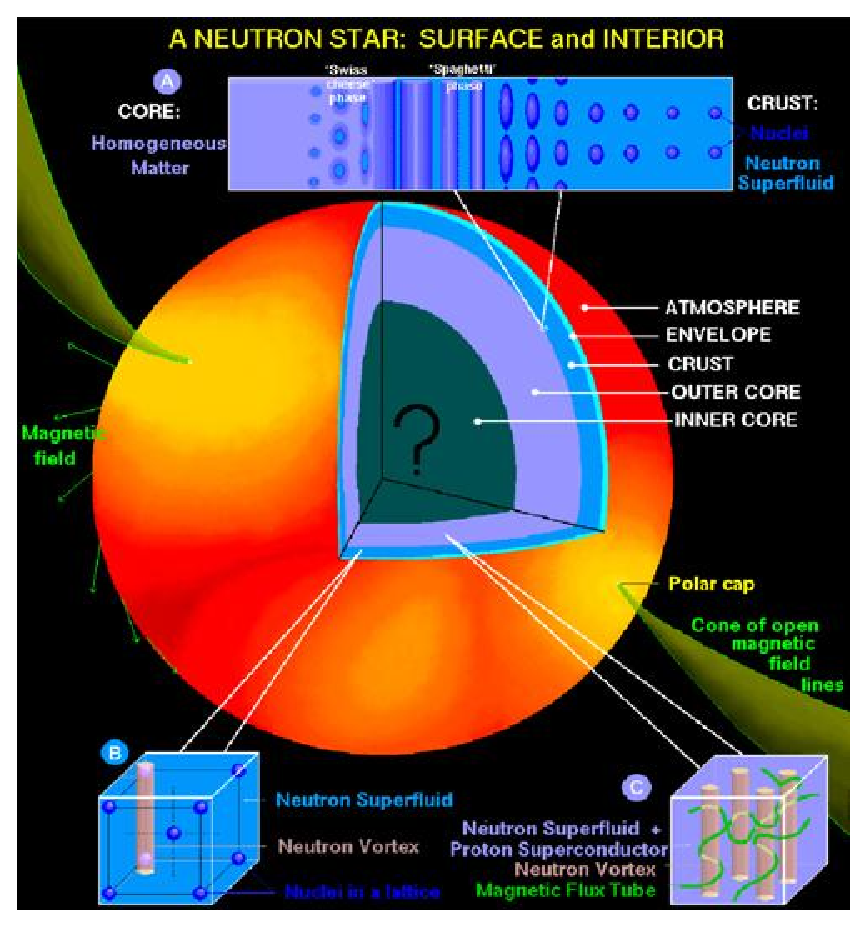
\includegraphics[height=80mm, width=80mm]{plots/a_neutron_star.eps}
	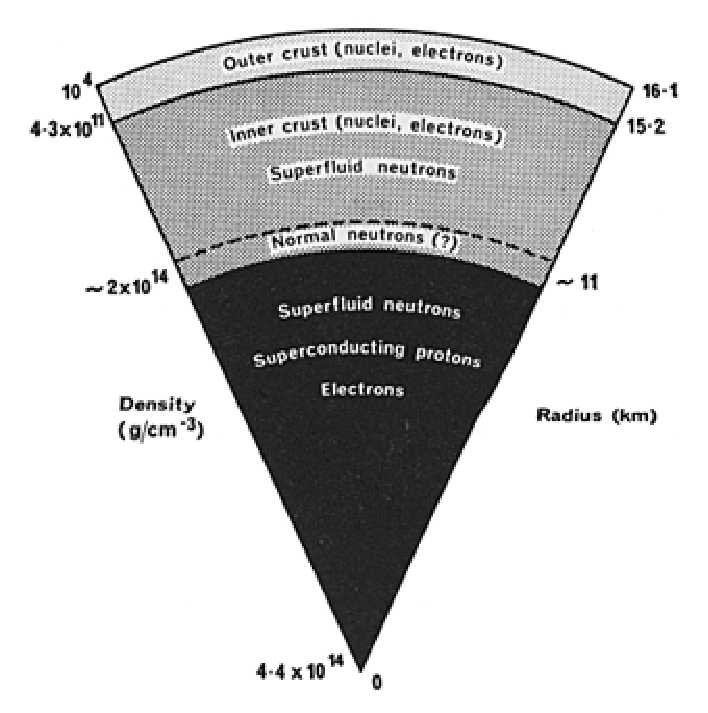
\includegraphics[height=80mm, width=60mm]{neutron_star_structure.eps}
	\caption{Hypothetical internal structures of a neutron star.  Left: theoretical neutron superfluid vortices and magnetic field lines (citation: Dany Page, \url{http://www.learner.org/courses/physics/visual/visual.html?shortname=a_neutron_star}). Right: putative depths of internal layers (citation: \url{http://heasarc.gsfc.nasa.gov/docs/objects/binaries/neutron_star_structure.html}).} 
        %CITE Possibly original Frank Shu? Fred would probably know, being a student of Frank
	\label{neutron_star_structure}
	\end{center}
	\end{figure}
        % INSERT A HIGHER QUALITY IMAGE HERE, POSSIBLY FROM ARUNAVA -- Done


Spinning neutron stars (NS)~\cite{Prix2006} motivate clear yet computationally challenging GW searches.
Perhaps one NS is born per century in the Milky Way~\cite{NarayanOstriker1990}.
In the solar-system reference frame, an isolated NS would emit a pure sine wave, as predicted by (with leading constant $G_C/c^4$) Equation~\ref{Fourier-domain-quadpole-eq}.
        One emission mechanism of gravitational radiation with amplitude $h_0$ from a NS is from a surface deformation defined as ellipticity $\epsilon$ (outer crust, Figure~\ref{neutron_star_structure}), leading to a quadrupole moment $I$~\cite{Zimmermann1979,LSCPulsar2006} and thus emission at frequency $f = 2\nu$, twice the NS spin frequency $\nu$:

        \begin{eqnarray}
        \epsilon &=& \frac{I_{xx} - I_{yy}}{I_{zz}}, \\
        h_0 &=& \frac{4 \pi^2 G_C}{c^4} \frac{I_{zz} f^2}{r} \epsilon.
        \label{cw_radiation_eps_eq}
        \end{eqnarray}

Emission might also arise from $r$-mode oscillations or free precession~\cite{Shawhan2010}.
Expected sensitivities for terrestrial interferometers, best around 100 Hz, highlight NS with comparable periods (millisecond pulsars) as suggestive targets.
For GWs from a rotating NS with a spin axis inclined at angle $\iota$ to an observer's line-of-sight, the relative polarization amplitudes~\cite{DergachevThesis} would be,

\begin{eqnarray} 
h_+ &=& \tfrac{1}{2} h_0 (1 + \cos^2 \iota),\\
h_\times &=& h_0 \cos \iota.
\end{eqnarray}

For $\cos \iota = 1$, where the spin axis is along the line of sight, gravitational waves will thus be circular polarized; $\cos \iota = 0$, an orthogonally-aligned spin axis, implies linear polarization.
Excepting the case of torque balance~\cite{PapaloizouPringle1978,Wagoner1984} in low-mass X-ray binary systems (LMXB), NS rotation frequency will decay due to gravitational radiation, yielding a relationship between the `spindown age'~\cite{Brady1998} $\tau$ and the gravitational radiation amplitude:

        \begin{eqnarray}
        \tau &=& -f / \dot{f}, \\
        h_0 &=& \frac{1}{r} \sqrt{\frac{5 G_C I_{zz}}{2 c^2 \tau}}.
        \end{eqnarray}

%            Continuous -- specifically, binary neutron stars and rate predictions. Describe archetypical search methods as in the 1998 analysis paper~\cite{Jaranowski1998}, the Abbott et al paper~\cite{LSCPulsar2006}, including StackSlide~\cite{LSCPulsarS4}, Einstein at Home~\cite{LSCEinsteinHome2009}, and the most interesting to date from Michigan, Vladimir's PowerFlux~\cite{LSCPowerFlux2009}. Discuss earlier results from the earliest period~\cite{Abbott2004} and an early search for Scorpius X-1~\cite{AbbottPulsar2006}. Reinhard Prix is probably another good source~\cite{Prix2006}.
Although pure sine waves are considerably simpler than the numerical relativistic templates needed for inspirals, the low expected $h_0$ and consequent long-duration integration needed to detect NS mean that the search over parameter space is extremely sensitive to mismatched templates.
This sensitivity implies that the algorithms must use fine-grained templates, necessitating long computational time.
Algorithms have been developed to search for these waves, starting from maximum likelihood estimates of isolated NS~\cite{Jaranowski1998}.
These have become progressively more sophisticated, incorporating barycentric solar-system correction~\cite{LSCPulsarS4}, distributed computing~\cite{LSCEinsteinHome2009}, and semi-coherent methods~\cite{LSCPowerFlux2009}.
Many isolated pulsars~\cite{Abbott2004,LSCPulsar2006}, including the Crab and Vela pulsar remnants~\cite{AasiPulsarInitialResults2014}, as well as the LMXB Scorpius X-1~\cite{AbbottPulsar2006} and the direction of the Galactic Center~\cite{AasiGalacticCenter2013} have been the target of these methods.

Many NS in known catalogs, such as ATNF (Australia Telescope National Facility~\cite{ManchesterATNF2005}), that pulsate in the LIGO frequency band are in binary systems.
This thesis describes, in Chapters~\ref{chap5} \& \ref{chap6} where this discussion continues, a computationally-efficient means, TwoSpect~\cite{GoetzTwoSpectMethods2011} of searching for NS in binary systems, particularly LMXBs. 
First, we discuss how gravitational wave interferometers sensitivity can be improved to make astronomy possible.

    \section{Laser Interferometer Gravitational-wave Observatories}
    \label{LIGO}
        
Design and construction of the Laser Interferometer Gravitational-wave Observatories required extensive prototyping and commissioning both during Initial LIGO~\cite{MavalvalaThesis,AdhikariThesis,BallmerThesis} and Enhanced LIGO~\cite{FrickeThesis,SmithThesis,DooleyThesis}.
The core features of interferometer design were established even before construction, summarized by Saulson~\cite{Saulson}, but many technical noise sources were encountered.
Motivations, fundamental noises, and the developments of commissioning all merit attention.

%        LIGO observatories. The most fun part to write. Cite Nergis Mavalvala~\cite{MavalvalaThesis}, Stefan Ballmer~\cite{BallmerThesis}, Rana Adhikari~\cite{AdhikariThesis}, Nicolas de Mateo Smith-Lefevbre~\cite{SmithThesis} and, of course, Peter Saulson~\cite{Saulson}.

        \subsection{From Weber bars to interferometry}
        \label{bars_to_interferometry}

Between the earliest interferometry of Michelson~\cite{michelson} and present-day LIGO came the resonant bar detectors of Joseph Weber~\cite{Weber1960}.
Bar detection of GWs developed rapidly through the 1960s, but contradictory results dampened enthusiasm~\cite{Saulson,CollinsGravityShadow}.
Nevertheless, great effort was devoted to technically excellent bars such as ALLEGRO, AURIGA, EXPLORER, NAUTILUS and NIOBE over the subsequent decades.
Meanwhile, prototypes by Rainer Weiss, Robert Forward~\cite{Forward1978}, Ronald Drever and many others demonstrated that interferometry could also achieve the sensitivities desired for gravitational wave detection.
Interferometry promised better fundamental noise sources and broadband operation, meaning that a single instrument could listen to a wider frequency band.
Xylophones of bars were proposed, but never built, that might scale the few Hz bandwidths of bars to the hundreds to thousands of Hz of interferometers.
Gravitational wave interferometry has carried the prospects for GW astronomy toward unprecedented levels of sensitivity, thanks to performance factors detailed in Section~\ref{methods}.

            %History lesson: Weber bars progress to interferometers. Use Saulson, but Nic's thesis has links to some of the original sources~\cite{Saulson},~\cite{SmithThesis}.           

        \subsection{Gravitational wave interferometry in theory}
        \label{methods}

% Maybe organize this section better

	Michelson invented modern interferometry~\cite{michelson} in his 1887 experiments with Morley to try to measure the velocity of the Earth with respect to the lumineferous ether.
Although commonly claimed to have spurred the work of Minkowski, the implications of this work for special relativity may not have been fully understood for several decades~\cite{CollinsGravityGhost}.
Yet the value of the experimental technique was undeniable.
Michelson \& Morley had invented an accurate relative phase-meter for light.

Existing GW observatories, at their cores, are also Michelson interferometers. 
In contemporary GW interferometers, monochromatic laser light (typically 1064 nm) is used.
This light is split into two equal beams by the beam-splitter, reflects off mirrors at the ends of two arms, X and Y, and returns to interfere at the beam-splitter after times $T_x$ and $T_y$.
The power $P$ at the beam-splitter output `dark' port, is by design near zero except when the measureable (e.g., ether, a GW, or other disturbance) causes a fringe shift $\Delta \phi$ related to the angular frequency $\omega$ of the light and the time-of-flight down the $x$ and $y$ arms, $T_x$ and $T_y$. 
Energy is conserved; the change of sign on the beam-splitter reflective surface means that destructive interference on the `dark' port implies constructive interference on the opposite 'bright' port.
Power is classically proportional~\cite{JacksonEM} to the squared electric field~\cite{Saulson}:

\begin{eqnarray}
P &=& \frac{\epsilon_0 c E_0^2}{2} \left| 1 - e^{i \Delta \phi}\right|^2 = 2 \epsilon_0 c E_0^2 (1 - \cos \Delta {\phi}),
\label{michelson-interferometry-eq}\\
\Delta \phi &=& 2\pi (L_s + L_0) /\lambda + \omega (T_y - T_x).
\end{eqnarray}

In Enhanced and Advanced LIGO, $L_s$ is known as the Schnupp asymmetry (a constant difference in arm length related to RF-modulated sidebands)~\cite{AdhikariThesis}, and $L_0$ is a smaller constant offset from a fringe to enable non-radio-frequency-modulated DC readout~\cite{FrickeThesis}.
A putative, even smaller `DARM' phase shift can read out $\omega (T_y -T_x)$, due to differential arm motion, encoding any time-varying GW signal in the relative time-of-flight between the arms. 
Operating near the maximum of $dP/d(\Delta\phi)$ would increase susceptibility to unwanted power fluctuations, so the interferometer was initially operated with radio-frequency modulation at minimum $dP/d(\Delta\phi)$ and  $P$ (a dark fringe), later changed to a slight offset and DC readout once the noise sources were better understood.

The GW sensitivity of the power $P$ can be directly improved by increasing effective laser power (e.g., a brighter laser or use of `power recycling'), and that of $\Delta \phi$ can be increased by making $T_{x,y}$ storage times longer (e.g., with Fabry-Perot cavities).
Doing so allows more accurate measurements of $P$ in the presence of shot noise (fluctuations in photon counting, entering via the $E_0$ term), radiation pressure (photon momentum-induced fluctuations in the mirrors causing changes in $T_y - T_x$), and other motions that change $\Delta \phi$ (such as thermal and seismic).
Yet these noise sources implicate quantum effects, and the photodiodes used to measure power do so with a certain quantum efficiency.
More realistic descriptions by Caves~\cite{Caves1980,Caves1981} clarify the quantum mechanical origin of shot and radiation pressure noise.
Quantum squeezing, the subject of Chapter~\ref{chap4}, can mimic the effect of higher power in Equation~\ref{michelson-interferometry-eq}.
GWs, eminently classical phenomena, are small enough in amplitude that quantum behavior is a key limit on detection.

Gravitational wave signals enter the interferometer by changing the spacetime curvature in the arms. 
In the simplest, linearized picture, the spacetime curvature arises from a GW with amplitude $h$ at frequency $f$.
When the GW is linearly polarized in $h_+$ and aligned with x-axis and y-axis arms of equal length $L$ (see~\cite{Jaranowski1998} for the antenna pattern correction when it is misaligned), it changes the time-of-flight in the arms according to Equation~\ref{GW-matrix-eq}:

\begin{eqnarray}
T_x = \int_0^{\frac{2L_x}{c}} \sqrt{|g_{xx}|} dt \approx \int_0^{\frac{2L_x}{c}} \left(1 - \frac{h_+ (t,x(t))}{2} \right) dt, \\
T_y = \int_0^{\frac{2L_y}{c}} \sqrt{|g_{yy}|} dt \approx \int_0^{\frac{2L_y}{c}} \left(1 + \frac{h_+ (t, y(t))}{2} \right) dt,
\end{eqnarray}

\noindent We have been able to neglect issues of the proper-time of the mirrors (as opposed to the photodiode) because the laser frequency $\omega$ is unchanged ($g_{tt} = 0$ in transverse-traceless gauge).
The mismatch in the integrals leads to a detectable time-varying signal,

\begin{equation}
\phi_{\textup{DARM}} \equiv \omega (T_y - T_x) = \omega \int_0^{\frac{2L}{c}} \frac{h_+ (t, x(t)) + h_+ (t, y(t))}{2} dt.
\end{equation}  

\noindent Measured by Equation~\ref{michelson-interferometry-eq}, $\phi_{\textup{DARM}}$ encodes the GW signal.
Comparing $\phi_{\textup{DARM}}$ from different observatories, or waiting while a single observatory is Doppler-modulated by terrestrial motion, can pinpoint the origin of such a signal.

We often assume that the time-of-flight is much less than the GW period, $T_{x,y} \ll 1/f$.
This assumption is easily relaxed by accounting for the destructive self-interference of the signal light from a high $f$ signal~\cite{Saulson}.
A straightforward interpretation emerges for a quasi-static plane-wave (when phase offset $2\pi L_0/\lambda \gg \phi_\textup{DARM}$) -- the interferometer linearly transduces GW strain (via $h_+ = \phi_\textup{DARM}c/(2L\omega)$) into power:

\begin{eqnarray}
%h_+ &=& \frac{c}{2 L \omega}\phi_\textup{DARM},\\
\frac{d P}{d h_+} &=& \frac{2L\omega}{c}\frac{dP}{d(\Delta\phi)} = 4 L\omega \epsilon_0 E_0^2 \sin \left(\frac{2\pi}{\lambda} (L_s+L_0) \right),\\
P &=& \left[ 4 L \omega \epsilon_0 E_0^2 \sin \left(\frac{2\pi}{\lambda} (L_s+L_0) \right) \right] h_+.
\label{strain-to-power-eq}
\end{eqnarray}

% DONE:           Why GW interferometers work. Null measurements, a zeroed operating point. 
%The specifics are best handled by Saulson~\cite{Saulson}. 

%The idea of a Pound-Drever-Hall lock is most elegantly explained by Black~\cite{PDHNotes}. Rai Weiss may have some neat details, possibly historical, albeit that it is in a presentation~\cite{LIGOWorks}. The details of Fabry-Perot cavities in LIGO are handled by Rakhmanov, Savage et al~\cite{ResonanceFP},~\cite{ResponsesFP}. i

%DONE: The motivation for the evolution to Enhanced LIGO and its DC readout methods is covered well in the corresponding CQG article~\cite{Fricke2009} and specific details of its construction and operation are in Tobin Fricke's thesis~\cite{FrickeThesis}.

            \subsection{Interferometer theory in practice}
            \label{interferometer_theory}

Interferometers transduce GW strain into power in a manner like Equation~\ref{strain-to-power-eq} only because they operate in a linearly-controlled regime~\cite{FrickeThesis} with noise sources surpressed as well as possible~\cite{Saulson,LIGOWorks}.
A complete discussion of noise is beyond our scope, but the key limits on a ground-based GW interferometer arise, for a facility in vacuum, from microseisms, gravitational gradients, thermal coating and thermal suspension noise, and quantum effects (radiation pressure and shot noise).

Seismic noise dominates the lowest frequences, and it is suppressed by use of servo controls, as well as by passive damping from pendula.
Each stage of a multi-stage pendulum reduces, for frequencies above its natural resonant frequency $f_0$, the coupling of seismic noise into the interferometer by a factor $(f/f_0)^2$.

Gravitational gradients due to clouds, human activity, and density fluctuations in the ground are an area of concern, but may be addressed through active feedforward servos~\cite{Driggers2012ActiveNoise}, as may magnetic couplings.

Thermal coating noise is reduced by using larger laser spot sizes on the surfaces of mirrors and optimizing the material properties of the coatings; the mirror itself must be made of a material with a high $Q$, such as fused silica, where $Q$ is the quality factor for internal oscillations.
Suspension thermal noise is also reduced by using high-$Q$ materials, as per the fluctuation-dissipation theorem~\cite{Saulson}.
These effects predominate in the logarithmic middle of LIGO's frequency range, often termed the `bucket'.

Shot noise is naively reduced by increasing laser power, which indeed yields improvements up to a point.
At high laser power, however, thermal distortions due to absorption in the mirrors are inevitable, leading to the need for thermal compensation systems~\cite{BallmerThesis}.
High laser power also buffets the mirrors with radiation pressure noise, requiring heavier mirrors.
Quantum squeezing can circumvent the issue of thermal distortions, but it too induces radiation pressure noise (typically worse, because the Heisenberg uncertainty area increases); a solution may be squeezing at high (shot noise-limited) frequencies and anti-squeezing at low (radiation pressure-limited) frequencies, as discussed in Chapter~\ref{chap4}.

%Noise sources dominate the 
%                GW interferometry theory: differential arm motion, key noise sources. 
%The main sources Saulson~\cite{Saulson} and Weiss~\cite{LIGOWorks}.
%                Here we discuss the key noises sources: seismic noise, thermal noise, and quantum (radiation pressure, shot noise).

GW interferometers on Earth are limited in size (thus storage time and strain sensitivity) by the planet's curvature (which couples vertical displacement noise into horizontal) as well as by finances. 
GEO600 uses delay lines, and the other interferometers use Fabry-Perot arms to extend the storage time of light.
Fabry-Perot arms with high-finesse~\cite{ResonanceFP,ResponsesFP} (roughly $137$ in Initial LIGO) are locked~\cite{PDHNotes} using the Pound-Drever-Hall (PDH) technique.
Elucidated below, electro-optic modulators (EOMs) provide a radio-frequency error signal for PDH locking the Fabry-Perot arms.

Figure~\ref{primary_eLIGO_optics} presents a schematic overview of the key systems in Enhanced LIGO.

\begin{figure}
\begin{center}
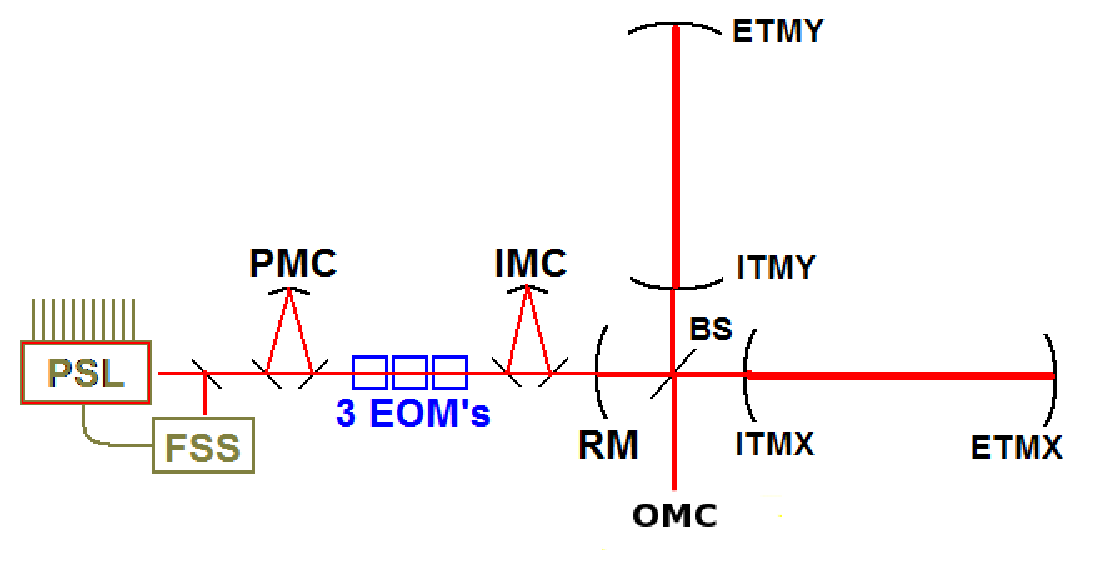
\includegraphics[height=90mm,width=148mm]{LIGODiagramnew.eps}
\caption{Enhanced LIGO primary systems and optics. From left, the phase-stablized laser (PSL) produces coherent light, kept at constant frequency by the frequency-stabilization servo (FSS). The pre-mode cleaner excludes non-Gaussian beamshapes, allowing only the $TEM_{00}$ mode to pass. The beam is the phase-modulated using three electro-optical modulators (EOMs) before being further shaped in the input mode cleaner (IMC). The beam passes through the power recycling mirror (RM) and is split at the beam-splitter (BS). Along the $X$ and $Y$ arms, light resonates in the Fabry-Perot cavity formed between the input test mass (ITM) mirror and the end test (mass) ETM mirror, before recombining at the beamsplitting. Any light with the same phase as before the arms is returned to the interferometer by the RM, but if phase-shifted, perhaps by a gravitational wave, it exits through the output mode cleaner (OMC): a photodiode just downstream of the OMC records the signal.}
\label{primary_eLIGO_optics}
\end{center}
\end{figure}

            \subsection{Observatory operation}
            \label{observatory_operation}

	\begin{figure}
	\begin{center}
	\includegraphics[height=111mm, width=148mm]{Screen_shot_2010-07-21_at_042516.eps}
	\caption{Screenshot of MEDM control panel. MEDM is a Motif Epic and Display Manager for EPICS, the Experimental Physics and Industrial Control System, which lets operators control LIGO. MEDM allows operators to run locking scripts as well as alignments and tests, and to activate and de-activate filters.}
	\label{ScreenshotMEDM}
	\end{center}
	\end{figure}

Satisfying the noise requirements above, the first-generation LIGO detector was designed with the following features:

\begin{itemize}
\item Power recycled Michelson interferometers with 4-km Fabry-Perot arms\footnote{A second 2-km interferometer was sited at Hanford as well during Initial LIGO.}
\item Hanford, Washington and Livington, Louisiana observatories
\item 4-km perpendicular beam tubes
\item $10^{−9}$ torr vacuum
\item 10 W Nd:YAG 1064 nm laser (Enhanced LIGO upgraded to 20 W)
\item 10-kg fused silica primary optics
\item 4-stage seismic isolation (including active hydraulics at Livingston)
\item Laser frequency stabilization
\item Angular sensing and control (wavefront sensors, optical levers)
\item Length sensing and control (magnet coils, common mode)
\item Pre- \& input-mode cleaning (Enhanced LIGO added output mode cleaning)
\item Power recycling
\item Digitally filtered servos and readout
\item RF heterodyne (Initial LIGO) or DC homodyne (Enhanced LIGO) readout
\end{itemize}

LIGO's digital systems were managed with MEDM and EPICS, seen in Figure~\ref{ScreenshotMEDM}.
Extensive effort on installation was required to attain the necessary angular, length, and auxiliary servo control needed for Initial LIGO operation~\cite{ReadoutGWA}.
Science Run 5 succeeded in obtaining the desired sensitivity and duty cycle.
Although the RF heterodyne technique\footnote{Curiously, the RF power sidebands as measured by the author were not always equal in the recycling cavity~\cite{MeadorsHanford2005}.} had good low-frequency sensitivity, it limited the shot noise performance compared to a DC homodyne instrument by a factor of $\sqrt{3/2}$, and squeezing was also easier in DC.
The switch to DC readout occured prior to S6, and in the leadup to that science run, substantial detector characterization was needed to understand the upgraded interferometer.

%                Operating LIGO: controls, Detector Characterization. One of the first sources from initial LIGO to read up on is a paper by Fritscel, Bork, Mavalvala et al~\cite{ReadoutGWA}. Initially this system made a detection based on heterodyne readout using GW sidebands, which, among other troubles, could be unequal in the recycling cavity~\cite{MeadorsHanford2005}.


\section{Detector characterization and development}
                \label{detchar}
            
%                    DetChar methods: omega scans, line hunting and glitches

\begin{figure}
\begin{center}
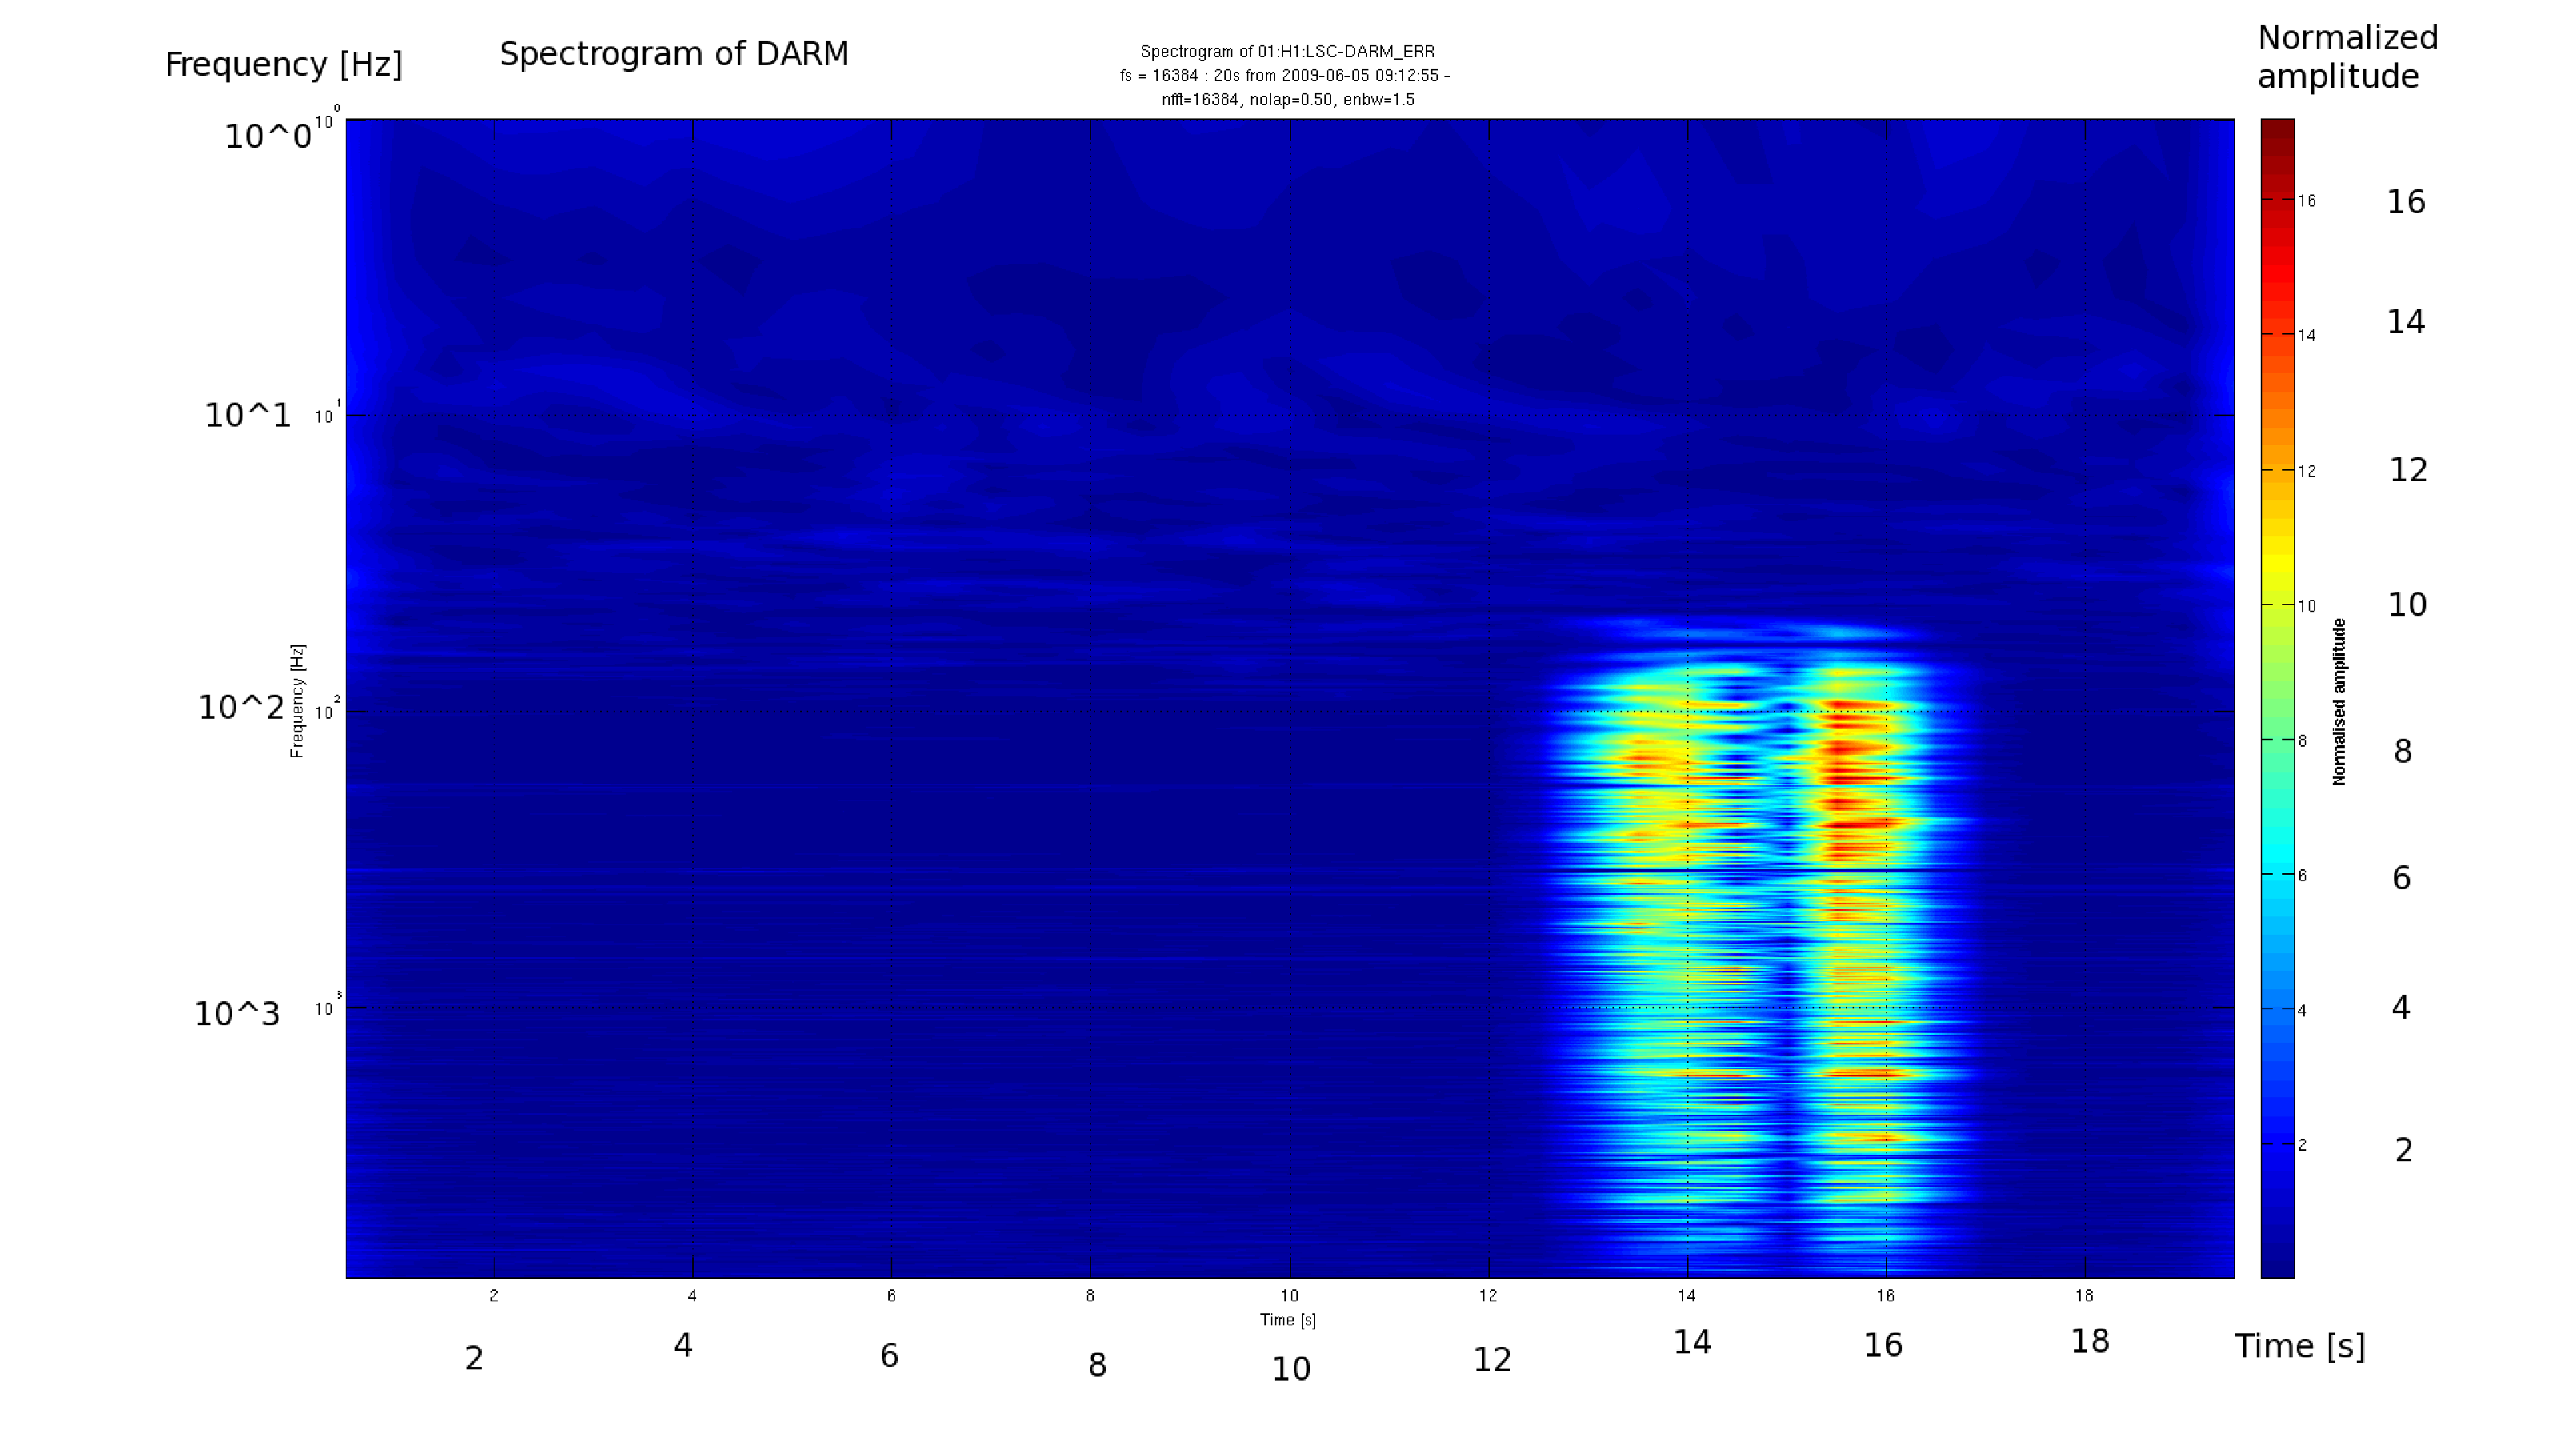
\includegraphics[height=111mm, width=148mm]{aglitch928228390_new.eps} 
\caption{Omega scan of an audible broadband glitch. Shortly before the start of Science Run 6, detector characterization took place to identify categories of glitches, such as the `gremlin', and to eliminate them. The burst group analysis pipeline, Omega, generated time-frequency spectrograms that made this identification easier. Glitches are a limiting factor in the identification of rare events and therefore of potential gravitational wave burst signals.}
\label{omega_scan_audible_glitch}
\end{center}
\end{figure}

Commissioning Enhanced LIGO in the three months encompassing the start of S6 around July 2009 required eliminating the residual noise sources lingering from installation. 
In particular, the Output Mode Cleaner~\cite{SmithThesis} was new, and its servo-locking scheme (involving both piezoelectric and thermal actuation) required some artistry.
DC readout generally increased the low-frequency noise floor.
New glitches sprang forth as a result, and the author's work at LIGO Hanford Observatory centered on identifying them.

Common tools for investigators on-site are both time-domain (DataViewer) and frequency-domain (Diagnostic Test Tools) data-plotters.
While those perspectives allowed diagnosis of at least one flaw in the interferometer's filters, a combined, spectrogrammatic view using the burst group's Omega analysis pipeline proved a needed third, unified view, seen in Figure~\ref{omega_scan_audible_glitch}.
This pipeline was run on many pre- and early-S6 glitches using a manual infrastructure\footnote{Omega scan diagnostics were later automated by Tomoki Isogai.}.

Effective engines for tracking and, preferably, eliminating glitches and persistent lines in the detector spectrum -- the process of detector characterization -- are critical to distinguishing rare events.

%My work on site included getting the Omega scan engine tested and running manual Omega scans in the first months of S6, July and August 2009. 
%See Figure~\ref{omega_scan_audible_glitch} for an example of the spectrograms this method was able to generate. These spectrograms helped categorize glitch sources and reduce them, to the benefit of the burst group in particular.
%Fortunately, this work was later automated thanks to Tomoki Isogai. 

                \subsection{Feedforward filtering}
                \label{feedforward_filters}

Feedback servos keep LIGO operational, holding the relative positions of the mirrors and auxiliary systems in stationary `lock' points.
Closing the loop in feedback requires a way to actuate a physical control signal to cancel out whatever influence is causing an error signal that pushes the system away from its lock point.
When this direct cancellation is not possible -- for instance, when ambient magnetic fields due to 60 Hz mains lines cannot be escaped -- feedforward remains.
Feedforward, an open-loop technique, be done purely in software, but it requires an accurate estimator for the influence of a noise source into the system.

In the case of Enhanced LIGO commissioning, an example was implemented with the aforementioned 60 Hz line using a magnetometer to supply the feedforward correction~\cite{SmithThesis}, which greatly enhanced sensitivity near the Crab pulsar frequency by suppressing magnetic-coupled noise.
Subsequently, into the following years, this author began to work on the long-known~\cite{AdhikariThesis,BallmerThesis} potential improvement from cancelling the influence of auxiliary length control noises.
Loops for nulling this effect exist, diagrammed in Figure~\ref{servo_loop_realtime}, but they require periodic retuning~\cite{KissellPRCMICH}.  
The direction of this work was to find an automated, and more precise, way to tune these servos.
A finely tuned servo filter was implemented in late September 2010\footnote{After, and unrelated to, the famed Big Dog blind injection event~\cite{Riles2013}.}.
This filter reduced the noisiest residual coupling, from the differential inner Fabry-Perot mirror motion to the differential arm motion that encodes strain, by almost an order of magnitude. 

                    %Example of feedforward: 60 Hz magnetometer. The only source that mentions this is, I think, Nic's thesis~\cite{SmithThesis}. Yet the most pertinent example is one that has long been applied to LIGO: MICH and PRC feedforward. The specific needed are mention in the thesis of Adhikari~\cite{AdhikariThesis} and Ballmer~\cite{BallmerThesis}, but immediately before Keita Kawabe and I began our project, these parameters had been tuned by Jeff Kissel~\cite{KissellPRCMICH}

	\begin{figure}
	\begin{center}
	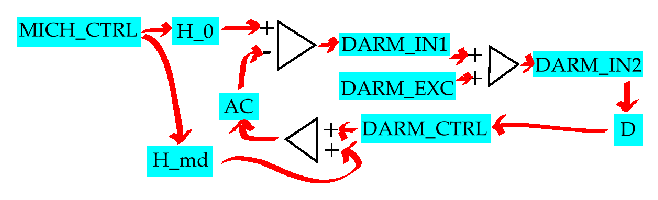
\includegraphics[height=80mm, width=148mm]{servo_loop.eps}
	\caption{Real-time servo loop diagram. The MICH\_CTRL signal can be though to leak into the true DARM signal via a transfer function, H\_0. (The letter `h' is typical for transfer functions as well as gravitational wave strain; coincidentally, this is a noise transfer into the channel for displacement, DARM, which is proportional to strain $h(t)$). H\_0 leaks into error signal, which is otherwise kept null thanks to the servo cancellation provided by DARM\_CTRL times a physical actuation function AC. The measured error signal is DARM\_IN1. If desired, an excitation can be supplied via DARM\_EXC for a sum of DARM\_IN2. This error signal passes though digital filters D to yield the aforementioned control signal DARM\_CTRL. The auxiliary length cancellation loop is simply adding H\_md to DARM\_CTRL in order to subtract out the corruption of H\_0.}
	\label{servo_loop_realtime}
	\end{center}
	\end{figure}

	\begin{figure}
	\begin{center}
	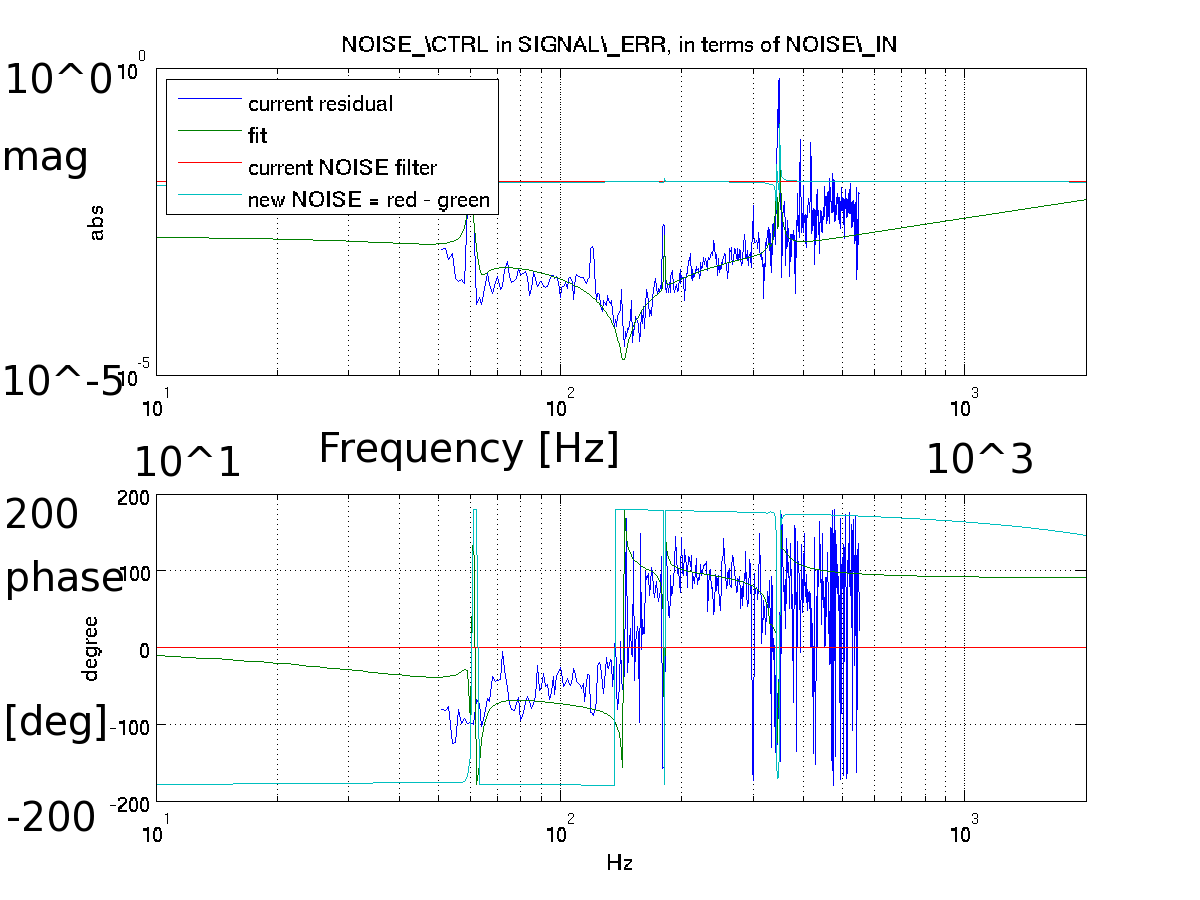
\includegraphics[height=111mm, width=148mm]{newNOISEfilter.eps}
	\caption{Real-time work on a LIGO noise filter. This Bode plot, made in Matlab, shows the correction to the existing MICH damping (cancellation) loop needed mid-2010, toward the end of Science Run 6. The correction is small, because the majority of the coupling fits the flat model expected from theory. This transfer function estimate suffices for post-factor correction. However, in order to be incorporated into the control scheme shown in Figure~\ref{servo_loop_realtime}, measurements of the open loop gain $G$ and actuation function AC are necessary to yield incorporate the filter correctly into the closed loop response.} 
	\label{newNOISEfilter}
	\end{center}
	\end{figure}

The closed loop gain mentioned in Figure~\ref{newNOISEfilter} is a function of frequency because it is a geometric sum of time $\tau$-delayed open loop gain responses by DARM\_CTRL to error signals from DARM\_ERR: $G_\textup{closed} = \lim_{p\rightarrow\infty} \Sigma_n^p G e^{i n \omega \tau} = \left(1 + G e^{i \omega \tau} \right)^{-1}$. 
Because MICH damping is summed with DARM\_CTRL, it picks up an additional factor of the actuation function AC for a net transfer function of $H_{md} G_\textup{closed}$AC in the closed loop. 
Thus, compared to an open-loop (e.g., post-facto) subtraction (effect estimated in Figure~\ref{filter_early}), a real-time servo will differ by a factor of $G_\textup{closed}$AC. 
See Chapter~\ref{chap3} for full details of open-loop subtraction and the extension to a post-facto, veto-safeguarded improvement in the sensitivity of all S6 data.

	\begin{figure}
	\begin{center}
	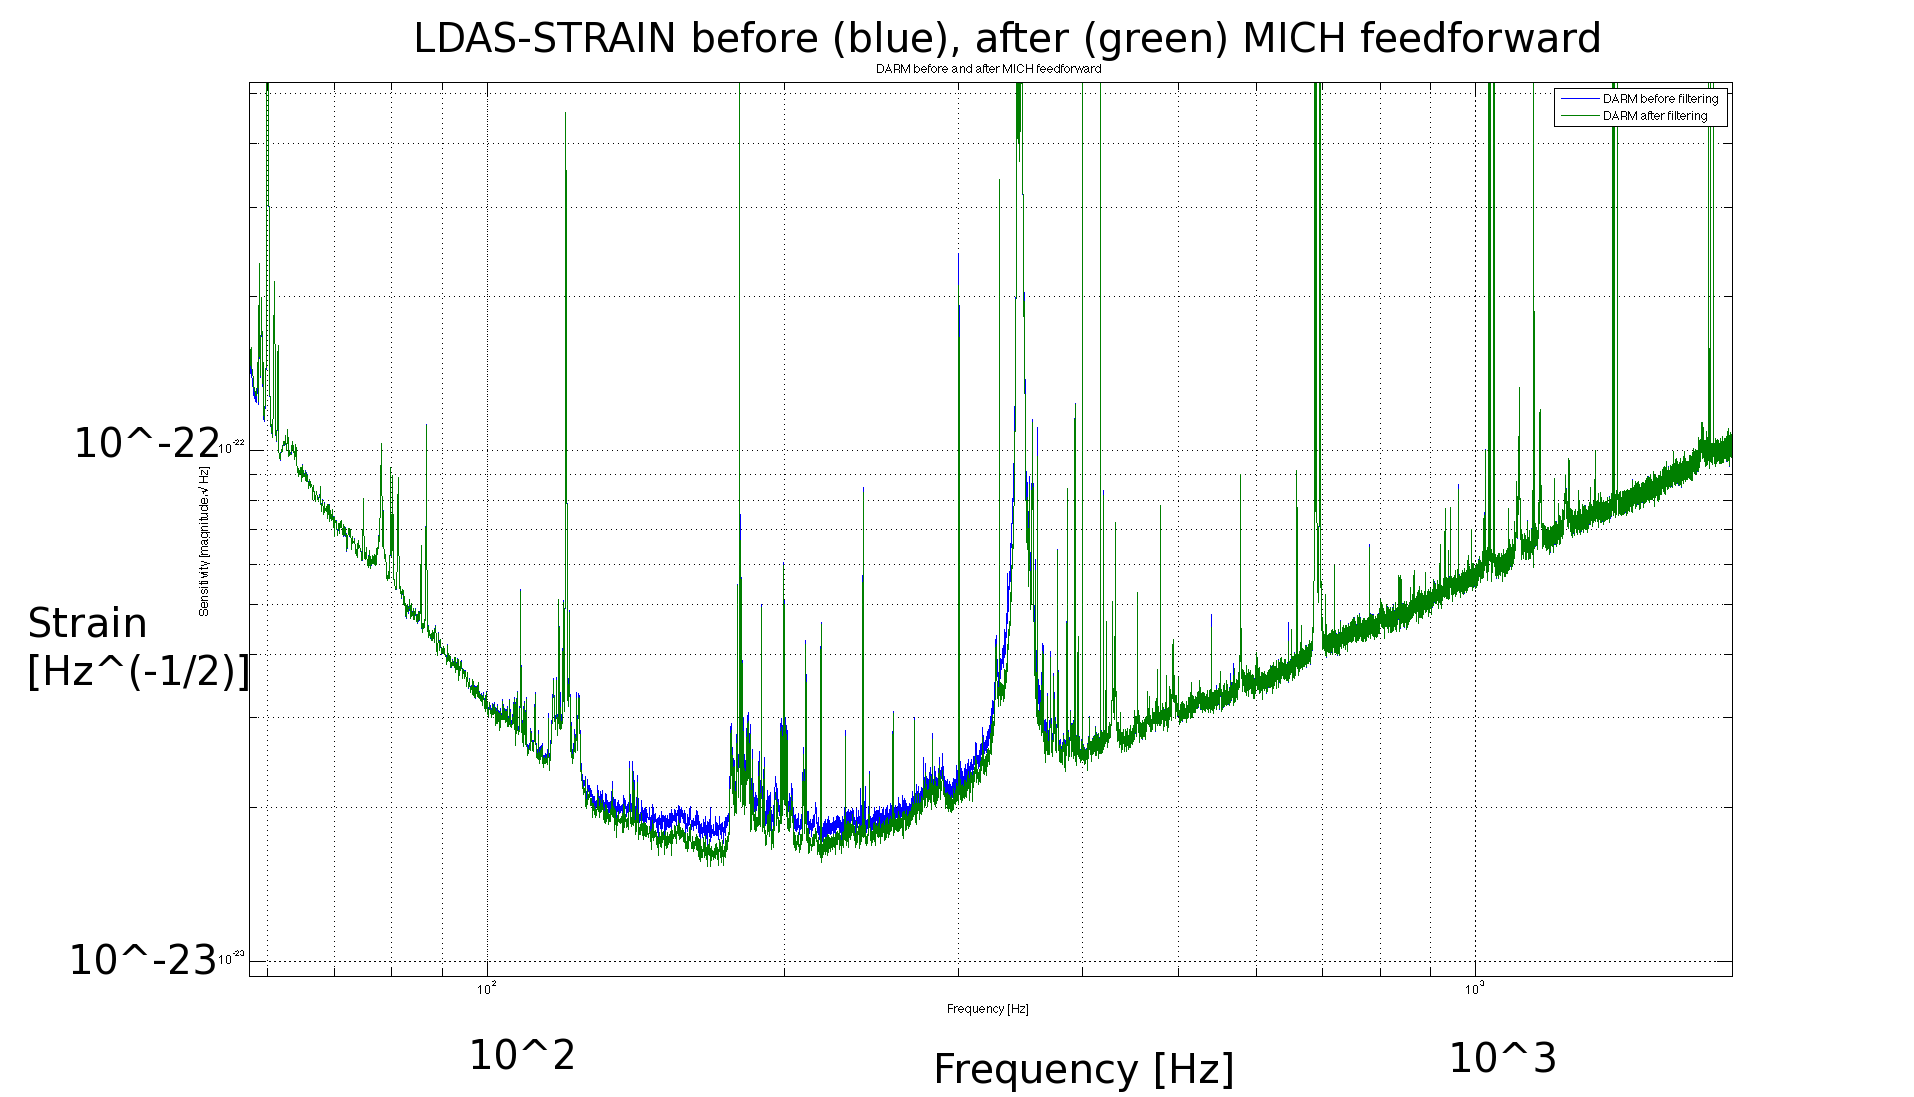
\includegraphics[height=90mm, width=148mm]{2011-03-08_filter-01.eps}
	\caption{Early work on post-facto noise filtering. After testing out MICH damping filters offline, post-facto, the correction factors for AC and $G_\textup{closed}$ were incorporated and the entire filter imported using Foton into the EPICS control system, where it was used real-time from the September equinox of 2010 until the end of Science Run 6.}
	\label{filter_early}
	\end{center}
	\end{figure}

                \subsection{Phase camera}
                \label{phase_camera}

Improving length control is intuitive, since length directly correlates with LIGO's inference of GW strain.
Angular control, however, is just as necessary: LIGO uses quadrature-photodiode wave-front sensors~\cite{MavalvalaThesis} to minimize misalignment.
Misalignment causes direct angle-to-length coupling, adding noise to the system by corrupting the phase measurement at readout; it also permits power fluctuations in the Fabry-Perot arms, reducing shot noise-limited performance and, when the relative power returning from the arms (the contrast defect) changes, directly corrupting the power measurement at readout~\cite{DooleyThesis}.
Maintaining lock also becomes hard if misalignment grows too severe.
Therefore more sophisticated systems have been researched in hopes of reducing angular fluctuations still further, including exploration of a phase camera at Michigan~\cite{DergachevThesis}.

%                    Future devices: overview of phase camera with Vladimir. Vladimir's thesis definitely talks about it~\cite{DergachevThesis}. We can discuss the fundamentals behind the need for angular stabilization and control from Nergis Mavalvala's thesis~\cite{MavalvalaThesis}, but we can refresh it with a modern reference from Kate Dooley's thesis~\cite{DooleyThesis}.
\begin{figure}
\begin{center}
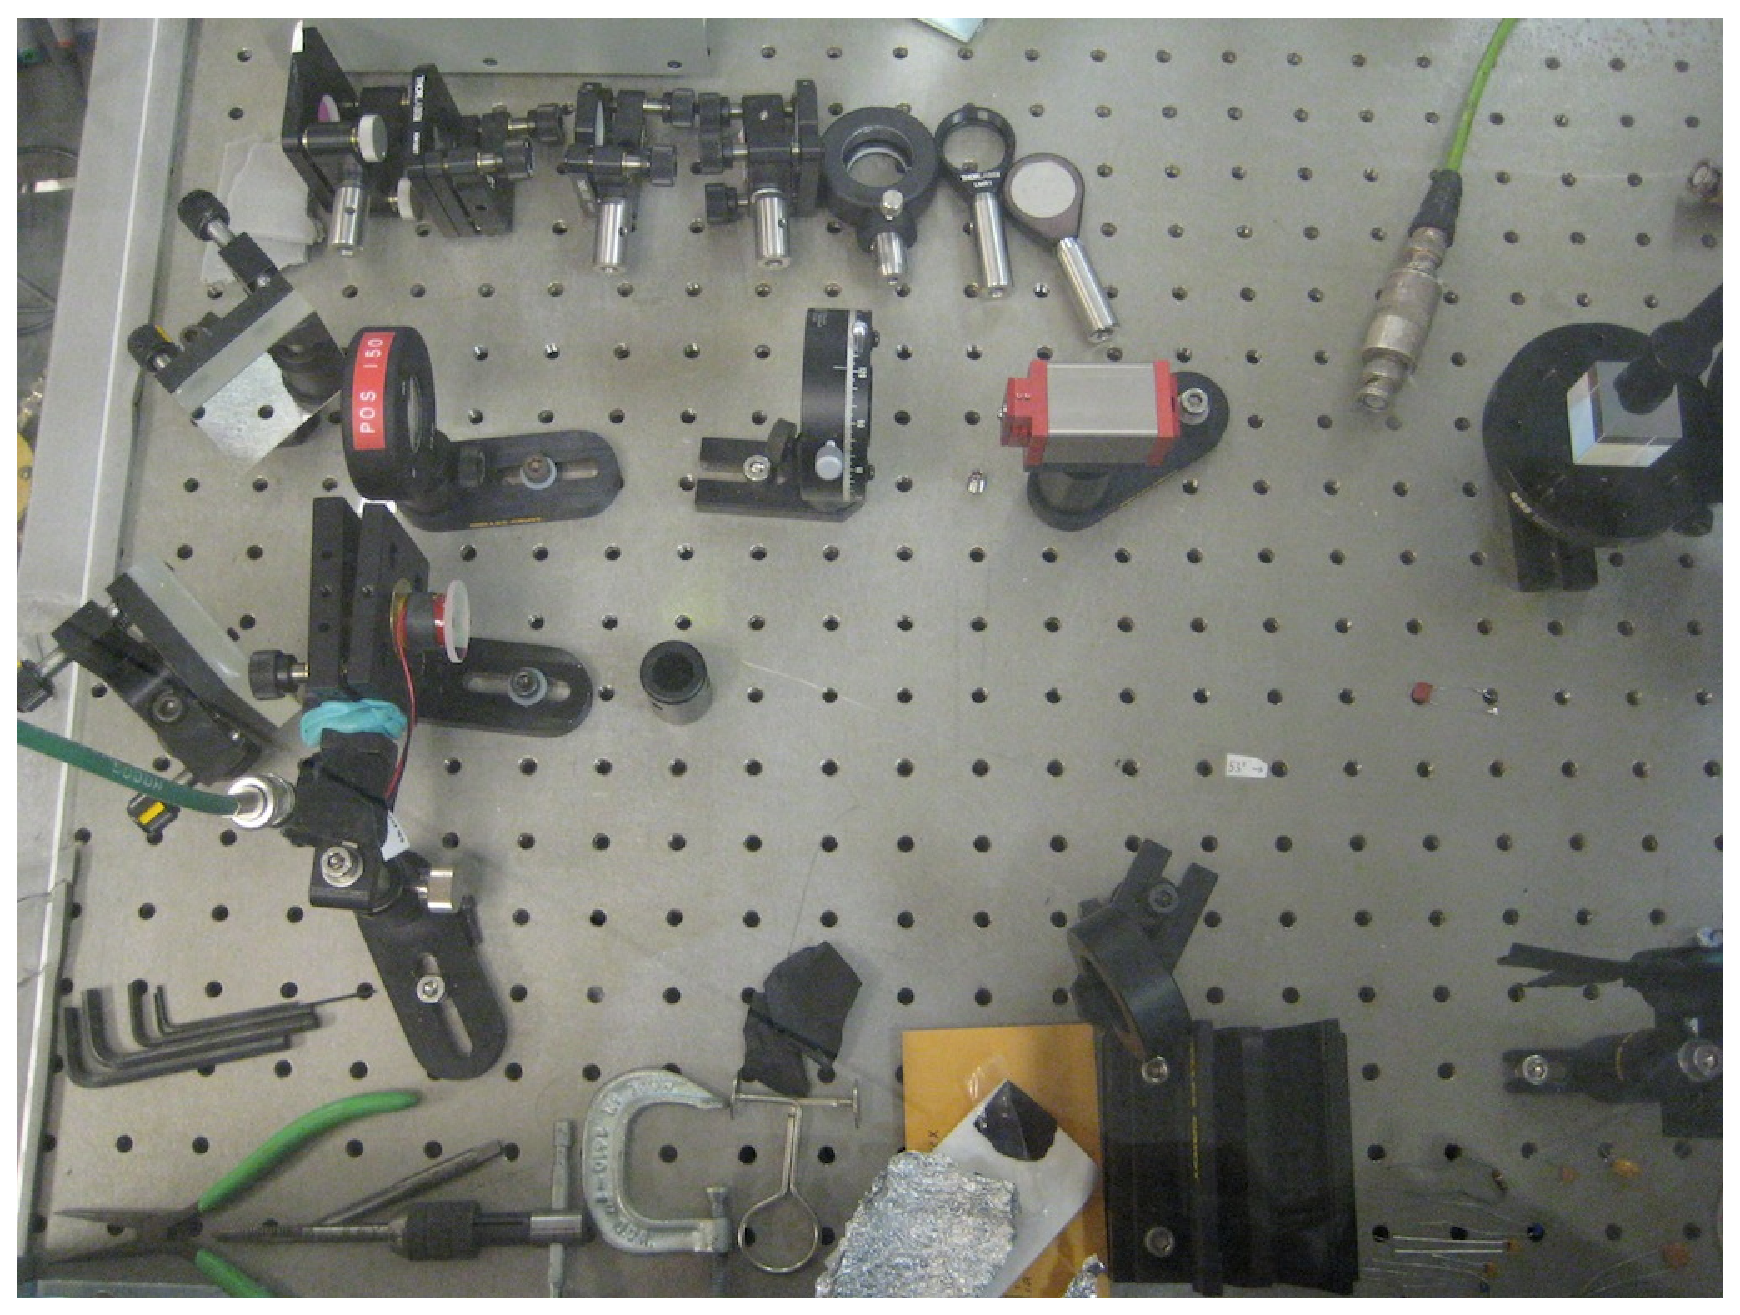
\includegraphics[height=111mm, width=148mm]{Optical_table_phase_camera.eps}
\caption{Optical table layout with Fabry-Perot cavity and Pound-Drever-Hall locking for phase camera. Faraday isolator and polarizing beam-splitter at upper right; piezo-electrically-actuated mirror at center left. Difficulties with stability, despite a plexiglass enclosure and floated table, meant that locks were fractions of a second at most, hampering efforts.}
\label{phase_camera_optical_table}
\end{center}
\end{figure}

Locking uses the Pound-Drever-Hall (PDH) method~\cite{PDHNotes,MavalvalaThesis}.
Mathematically, the method assumes two mirrors: an input, with amplitude reflectivity $r_1$, and an end, with amplitude reflectivity $r_2$.
Upon the input mirror is incident a coherent electric field, due to light, $E_\textup{inc}$ at frequency $\omega_0$. A field $E_{\textup{refl}}$ is reflected.
The key to the technique is that the incident electric field is phase modulated by an amplitude $\Gamma$ with modulation frequency $\Omega$, by a device such as an electro-optic modulator (EOM, e.g., a Pockels cell).
Typically this modulation is done at radio-frequency.
This EOM modulates an electric field of amplitude $E_0$ into higher and lower frequency sidebands, amplitude $E_+$ and $E_-$, as determined by expansion in Bessel functions $J_n(\Gamma)$ -- higher order sidebands exist at smaller amplitudes.
From the reflected signal, then, the intensity $I$ encodes an error signal of the arm length $l$, for given light wavenumber $k = \omega / c$, at the modulation frequency (aside from additional signals at DC and at 2$f$):

\begin{eqnarray}
E_{\textup{refl}} &=& \frac{r_1 - r_2 e^{-2 i k l}}{1 - r_1 r_2 e^{-2 i k l}} E_\textup{inc},\\
E_\textup{inc} &=& E_0 e^{i \Gamma \cos \left( \Omega t \right)} \approx E_0 e^{i \omega_0 t} \left[ J_0 (\Gamma) + J_1 (\Gamma) e^{i\Omega t} + J_{-1} (\Gamma) e^{-i \Omega t} \right],\\
E_\textup{refl} &\approx& e^{i \omega_0 t} \left[ E_0^\textup{refl} + E_+^\textup{refl} e^{i\Omega t} + E_-^\textup{refl} e^{-i \Omega t}\right],
\end{eqnarray}
\begin{equation}
\begin{split}
I =& \left[ |E_0|^2 + |E_+|^2 + |E_-|^2\right] + \\ 
  & \left[(E_0^* E_+ + E_0 E^+_-)e^{i\Omega t} +\textup{C.C.} \right] + \\
  &\left[E_+ E_-^* e^{2i\Omega t} +\textup{C.C.} \right].
\end{split}
\end{equation}

Radio-frequency photodiodes are generally needed to record this intensity with its modulation.
Typically, the photodiode current is demodulated with a mixer that uses as local oscillator the same sine wave that drives the Pockels cell EOM phase modulation.
Alternative photoresistor readouts were explored in hopes that they might have faster response times since the standard electronics references were compiled~\cite{HorowitzHill1989,Simpson}, because of their potential desirability for a low-cost many-pixel readout.
Part of this author's work included a Spice simulation and physical construction of a photoresistor circuit.
Sadly, the inexpensive photoresistors used had rise times of milliseconds, far too slow for a direct RF readout scheme. 
This result refocused attention on photodiodes.

%The electronics development were guided by Horowitz and Hill~\cite{HorowitzHill1989} as well as by Simpson~\cite{Simpson}.
Using the usual RF photodiode, a Fabry-Perot cavity was built prior to this author's work, seen in Figure~\ref{phase_camera_optical_table}.
My efforts began with characterizing the RF electronics of the analog locking system.
A signal analyzer helped re-select a cable of appropriate length and phase delay for the system. 
Numerous attempts to stabilize the cavity and derive a useful PDH locking signal were made.
The laser was upgraded from Helium-Neon to solid-state.
A faulty EOM replaced, and its frequency response was studied by this author (helped by Gustafson) to choose a better modulation frequency where the EOM could supply adequate modulation depth.
Unfortunately, locks proved too fleeting to pursue a program of phase camera angular measurements.
% This program would involve intentionally misalignment and correction
Much progress nonetheless was made by Dergachev in realizing effective methods of high-speed digitization of the RF-modulated signal in free space~\cite{DergachevThesis}.
The full program, for investigating a multi-pixel RF sensor with digital (in-software) demodulation, has yet to be realized.
%See Figure~\ref{phase_camera_optical_table} for a picture of the cavity as built.


        \subsection{Advanced observatories and beyond}
        \label{advanced}
  
            %Advanced LIGO and beyond -- squeezing and prospects?
%DUSEL, 
	Advanced LIGO (aLIGO)~\cite{aLIGOrefDesign,aLIGOsysDesign} is intended to improve upon the first-generation LIGO inspiral range tenfold, to 200 Mpc.
To accomplish this, it simultaneously must lower the noise floor at the most sensitive frequencies, to a strain noise  $4\times10^{-24}/\sqrt{\textup{Hz}}$, and push the low-frequency wall of seismic noise down, so that frequencies as low as 10 Hz (rather than about 50 Hz) can be probed.
%While maintained in the same vacuum envelope,
The aLIGO optical systems are far superior to those of initial LIGO.
The 10-kg fused silica test mass mirrors have been upgraded to 40 kg for better radiation pressure performance.
Fused silica fibers with high $Q$ suspend the mirrors, instead of steel piano wire; fibers are welded directly to the test mass.
Rather than a single pendulum, each test mass sits at the bottom of a four-stage `quad', actively-servoed pendulum chain, reducing seismic noise, in principle, by a factor of $(f/f_0)^8$.
The quad pendulum itself is attached to a new in-vacuum seismic isolation table (similar tables hold the auxiliary optics).
These test masses indeed need to be heavier.
Laser power has increased from 20 W in Enhanced LIGO to 200 W in aLIGO.
Fabry-Perot arm cavity finesse has also increased, raising the stored arm power.
The arm cavities can be locked independently of each other and brought into the Michelson interferometer gradually, which should improve ease of use, allow quick recovery from lock-losses, and thereby improve reliable duty cycle, coupled with other system-wide improvements in control architecture.
Resonant sideband extraction is one of the most inventive changes, adding an additional signal recycling mirror to the optical configuration, which allows tuning the cavity pole of the Fabry-Perot arms and trading between different levels of high- and- medium-frequency shot noise-limited performance.

Although not part of the reference design, the success of the LIGO Hanford squeezing experiment~\cite{BarsottiNatureSqueezing,ChuaBackscatteredLight,DwyerPhaseNoise} noted in Chapter~\ref{chap4} make quantum optics a likely feature of any enhanced follow-up.

Once commissioned, aLIGO's second-generation design should make possible detections at the rate of 40 per year~\cite{AbadieRates2010}. 
Hanford and Livingston have both upgraded their 4 km interferometers and have begun commissioning.
The 2-km Hanford interferometer had been intended to be upgraded, but its optics have found a new and likely more useful propect -- part of the growing network of observatories described in Section~\ref{worldwide}.

        \subsection{Worldwide network}
        \label{worldwide}
 
Gravitational wave signals are new to astronomy.
It has long been recognized that multiple observatories with independent confirmation of a signal would be more persuasive evidence of detection than an isolated site.
Yet even once the field is established, additional observatories will permit better science.
Sky localization of inspiral and burst sources relies on relative arrival times of a GW signal~\cite{Saulson}.
Multiple, widely separated observatories give the best baseline.
Moreover, the data for continuous wave searches from separate sites can often be coherently combined to yield a quieter noise spectrum.
LIGO is fortunate thus not to be alone in the pursuit of gravitational wave astronomy.

%The second, 2-km Hanford interferometer will likely not be upgraded to aLIGO.
            %Allies: 
Optics for a third interferometer will form the core of the nascent LIGO India project~\cite{IyerIndia2011}, which will dramatically improve the accuracy of sky position measurements for gravitational wave transients.
In Japan, KAGRA~\cite{Kuroda2010} is being built; when completed with sapphire mirrors and cryogenic systems, it should reach comparable sensitivity to the LIGO interferometers.
Advanced VIRGO~\cite{Acernese2009} benefits from the first-generation superattenuator's superb seismic isolation performance; from it will be suspended new optics that reflect a more powerful beam.
Together, these second-generation ground-based interferometers should suffice to make direct detection of gravitational waves a reality.

Around the same time as these observatories make first detection, an entirely different technique of GW astronomy, pulsar timing~\cite{Hobbs2010}, may open up vastly lower frequencies ($\mathcal{O}(10^{-9})$ Hz).
The two techniques should provide complementary information about the gravitational sky, as distinctive as gamma ray telescopes are from radio.

Yet GW astronomy would become a true precision science if a third generation of instruments followed.
Third-generation interferometry could take place underground, either in proposed American DUSEL or the European Einstein Telescope~\cite{Punturo2010}, potentially with xylophone interferometers tuned to optimize sensitivity in different frequency bands.
Prospects in space appear even grander in the long-term, despite short-term setbacks. 
Following NASA withdrawal from the Laser Interferometer Space Antenna, LISA, in 2011, the European Space Agency has made a concerted push to launch LISA Pathfinder in 2015, with plans for a somewhat-reduced yet very capable eLISA in coming decades~\cite{Vitale2014}.
If eLISA launches, it may open the way for measurements of the most elusive gravitational signature: the background of the universe itself.
Both the DeciHertz Gravitational Observatory (DECIGO)~\cite{Ando2010} and Big Bang Observer (BBO)~\cite{Harry2006} proposals could, by midcentury, open up a vision of the cosmos in its earliest days.
%LISA Pathfinder to launch in 2015 and eLISA to follolw~\cite{Vitale2014}

    \section{Summary}
    \label{intro_summary}
 
        %Summary: strong motivation and instruments, need to find evidence of GW.    

Initial LIGO, during the science run S6, would have been able to see the coalescence of two neutrons stars at about twenty Megaparsecs, out in the Virgo cluster of galaxies, from sixty-five million years ago, when dinosaurs still walked the Earth. 
In the first week of aLIGO lock at Livingston, following Memorial Day 2014, aLIGO had a temporal range extending only as far back as when early humans began their diaspora from Africa -- a terrestrial parallel to the expansion of the cosmos.
Just after Labor Day, aLIGO had exceeded the range of S6.
Progress on aLIGO has been swift.
When completed, the Hanford and Livingston second-generation interferometers should see back ten times beyond what S6 could, six hundred and fifty million years, to before the Cambrian explosion of life.
Perhaps in the third or fourth generation of interferometers, our view of the gravitational sky may stretch back to the age of the observable universe.
Even then, we will not have seen all that can be seen.
With the two long-range forces of the universe, electromagnetism and gravitation, giving two complementary views of spacetime, we still must build great machines to explore the sights they show, we must understand what we are seeing, and we must propagate that understanding. 

This thesis is a prelude to those efforts, from the building of the quantum optical squeezer, and the feedforward regression and continuous waves binary search, to our public interferometer exhibitions.   
Feedforward regression provides a microcosm of the complexities of gravitational wave interferometry, so there we will begin.


            
%        --------------------
%
%	Here is a sample chapter file. The chapters of the thesis
%	should be saved to seperate files such as
%	\textit{chapter1.tex}. In the file \textit{thesis.tex} the
%	\textit{input} command then includes these chapters into the
%	thesis. Note that none of the chapter files need any headers.
%	This header for each of these files is contained in
%	\textit{thesis.tex}. The file \textit{thesis.tex} also
%	includes the numbers system for the sections, figures,
%	theorems lemmas etc...

%\section{Sample Section}
%\label{sample_section}
%
%	This is what a sample section looks like. Let's conclude this
%	section with a sample theorem statement and proof.
%
%	\begin{theorem}
%	\label{sample_theorem}
%	The are an infinite number of prime numbers
%	\end{theorem}
%
%	\emph{Proof:} On the contrary assume there are a finite number
%	of primes $P_1, P_2, ... P_n$. Consider $\mathcal{P} = P_1 P_2
%	\cdots P_n+1$. $\mathcal{P}$ is not divisible by any of the
%	primes in our finite set. (Contradiction) $\square$
  


% Feedforward (Auxiliary MICH-PRC Subtraction)
\chapter{Squeezing: Quantum Vacuum Phase Noise}
\label{chap3}


    (Fill in bits about the squeezer)

    \section{Squeezing theory}
    \label{squeezing_theory}

        Squeezing theory.

        \subsection{Quantum shot noise and radiation pressure}
        \label{quantum_noise}

            Carlton Caves, quantum shot noise and radiation pressure.

%\begin{frame}{Squeezing introduction}

%\begin{definition}
Altering $\Delta E\Delta\phi$ uncertainty for the electromagnetic
field
%\end{definition}
\begin{itemize}
\item Demonstrated first at GEO 600, then LIGO Hanford (H1)\end{itemize}
\begin{theorem}
Shot noise arises from quantum operators (Caves 1980, 1981)\end{theorem}
\begin{itemize}
\item Vacuum fluctuations couple through anti-symmetric port
\item \emph{Squeeze }the $\overrightarrow{E}$ field uncertainty ellipse
\item Angle $\theta$, factor $r$, creation operator $a$, squeeze operator
$S$:
\end{itemize}

\[
S(\zeta)=\exp[\frac{1}{2}\zeta^{*}a^{2}-\frac{1}{2}\zeta(a^{\dagger})^{2}],\;\zeta=re^{i\theta}
\]



Squeezed state made with


optical parameter oscillator, 2nd harmonic generator


\textbf{Shot noise reduced by $e^{-r}$}


\[
\]




        \subsection{Problems with lasers: thermal compensation}
        \label{TCS}

            Experience (some firsthand) with thermal compensation.

        \subsection{Squeezing filter cavities against alternatives}
        \label{third-gen_squeezing}

    \section{LIGO Hanford Observatory quantum vacuum squeezing}
    \label{LHO_squeeze}

        Quantum vacuum squeezing at LIGO Hanford Observatory. Naturally, a great deal of description and background will come from Sheila Dwyer's thesis~\cite{DwyerThesis} and Sheon Chua's thesis~\cite{ChuaThesis}.

        \subsection{Collaboration and contributions}
        \label{contributions}

            Contributions: table, in-vacuum installation, electronics, range est.

            \subsubsection{Optical table support assembly}
            \label{table_legs}

                Table legs (me) and results of Sheon and Robert's shakers.

		Here might be good place to put old AutoCAD drawings to use.

            \subsubsection{Faraday isolator measurement}
            \label{Faraday}

                Faraday isolator measurement (me with Keita, Matt, Lisa).

		What were the results of the measurement? Show e-log entries, comment on in-and-out-of-vacuum performance and what it says about the need for low loss to be a top priority in future squeezing efforts.

            \subsubsection{In-vacuum installation}
            \label{In-vacuum}

                In-vacuum Faraday and baffle installation with "".

                Show pictures of the installation, connect to the issues with stray and perhaps backscattered light.

		Discuss the repair of the output mode cleaner, which is mentioned (citation 50) in Nic's thesis~\cite{SmithThesis}. The technical report corresponding to it is by Waldman and Chua~\cite{Waldman2011}.

            \subsubsection{Data digitization}
            \label{data_digitization}

                Electronic cabling and analog-to-digital converter installation.

		May want helpful diagram.



%\end{frame}

%\begin{frame}{Squeezing large interferometers}


\begin{figure}
%\protect\caption{\protect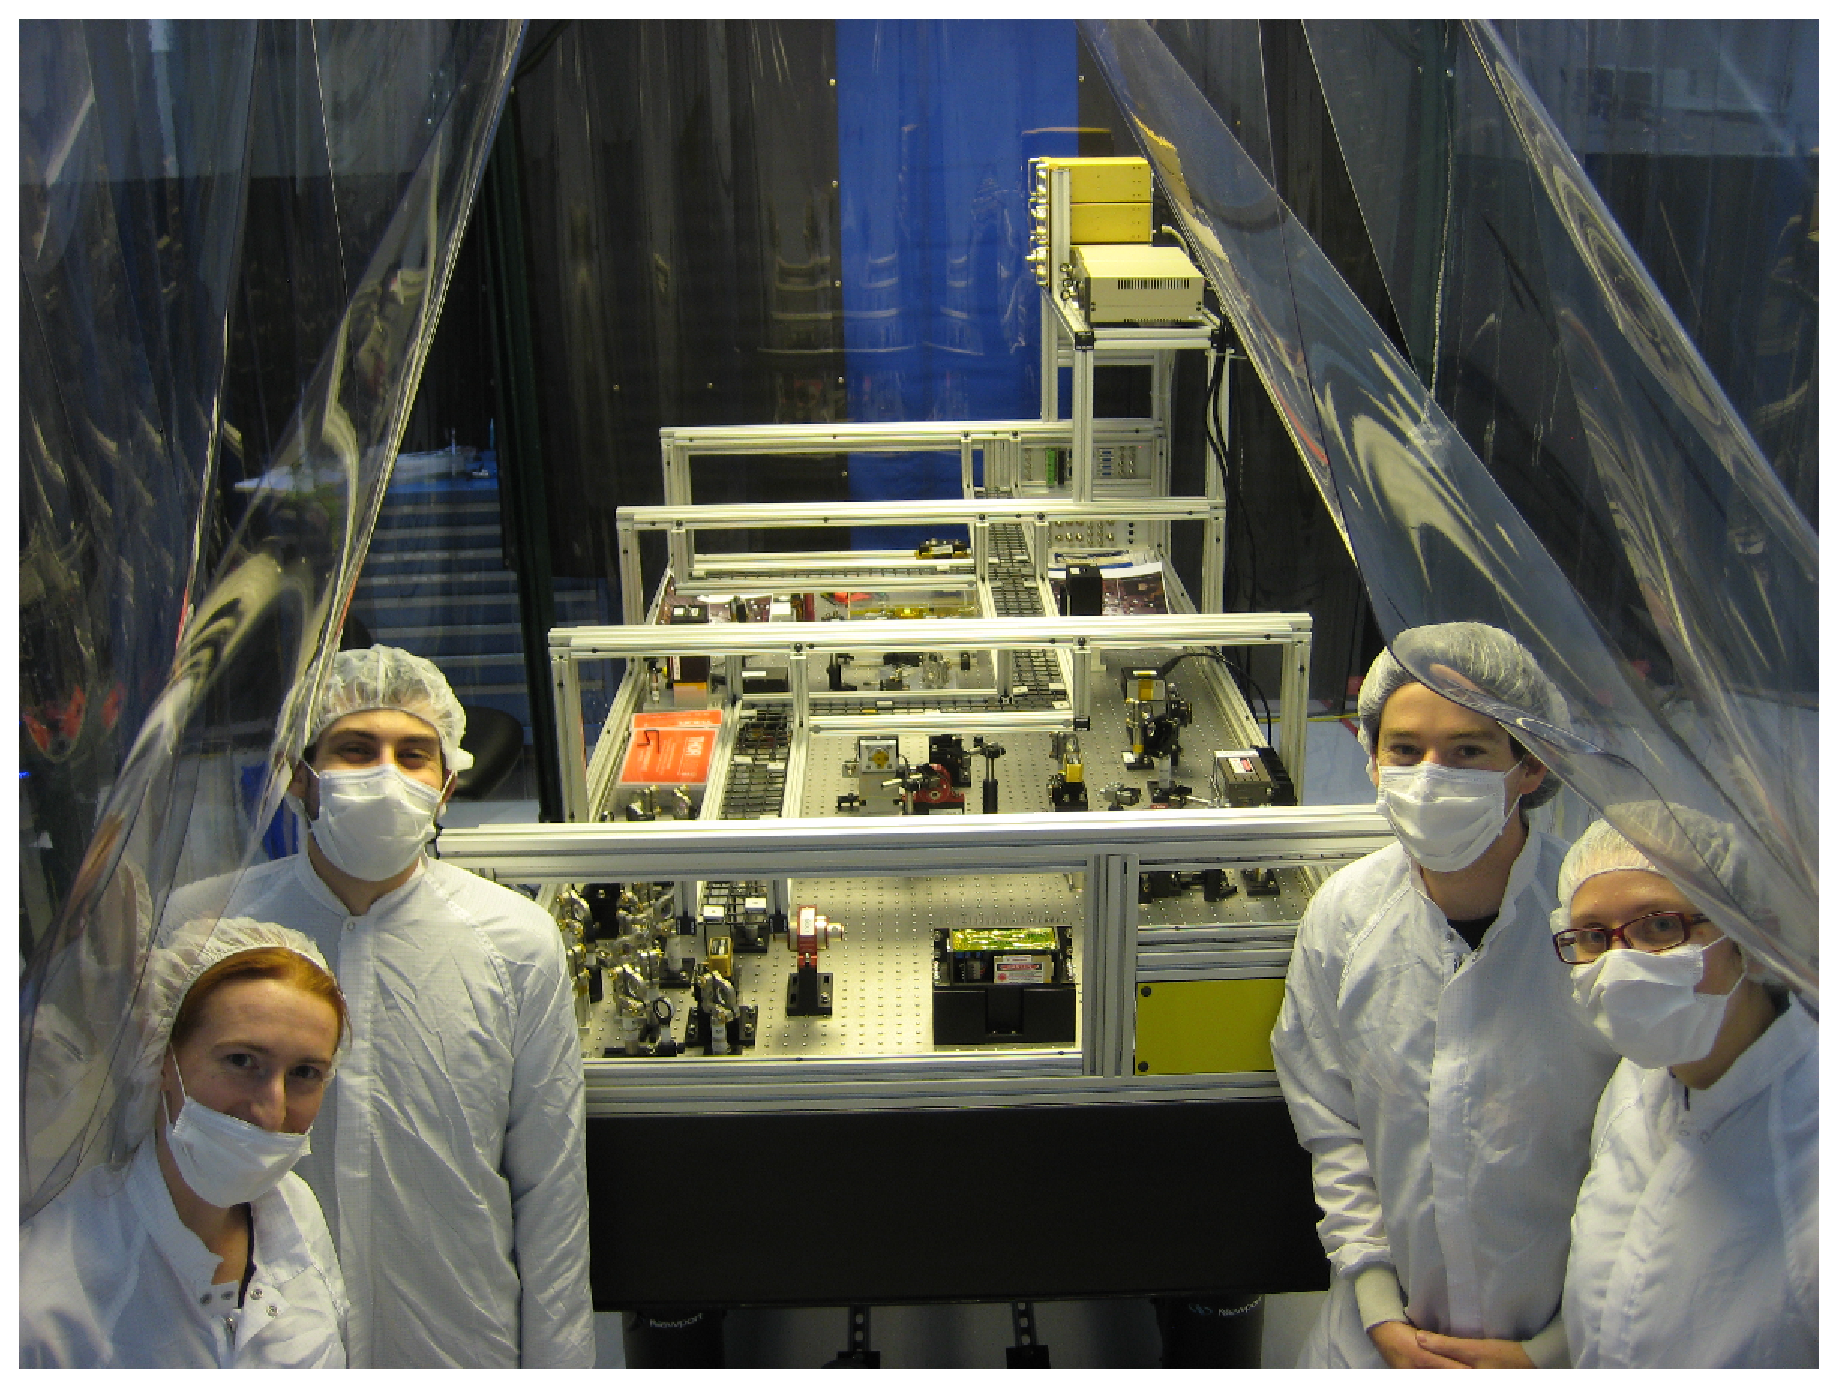
\includegraphics[width=0.33\paperwidth]{lisabar-1289966130}}
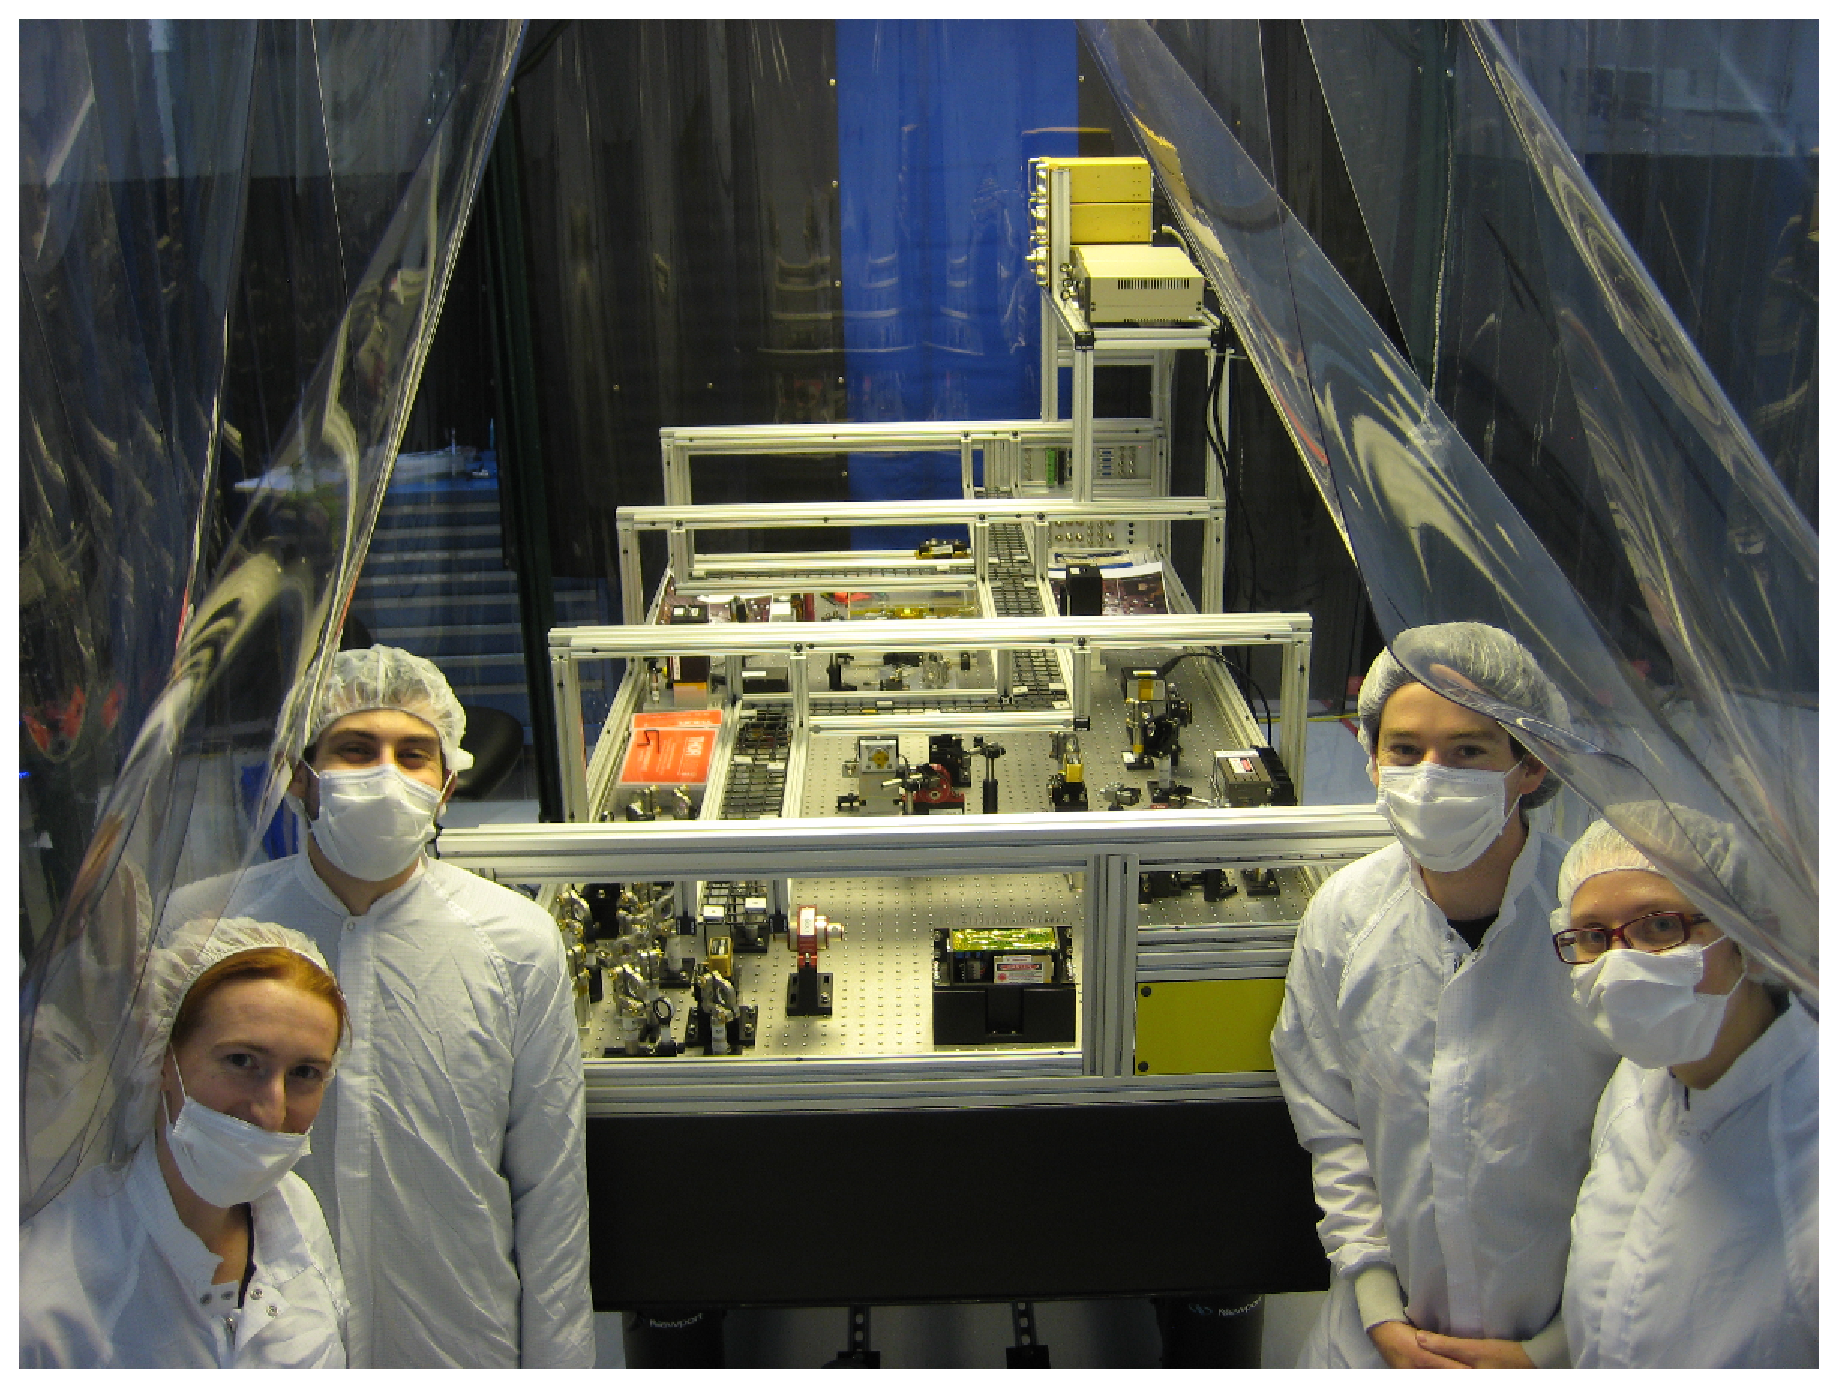
\includegraphics[width=0.6\paperwidth]{lisabar-1289966130.eps}


%\protect\caption{\protect\includegraphics[width=0.33\paperwidth]{lisabar-1300943141}}


\caption{Image by Lisa Barsotti in Hanford eLog
\newline CC from LL, Dwyer, Barsotti, Mow-Lowry, Meadors
}
\end{figure}
\begin{figure}
\includegraphics[width=0.6\paperwidth]{lisabar-1300943141.eps}
\caption{Table legs (\& helped w/ Faraday isolator, data channels)
}
\end{figure}


%\end{frame}

%\begin{frame}{Squeezing's scientific benefit}
\subsection{Squeezing's scientific benefit}


\begin{figure}
%\protect\caption{\protect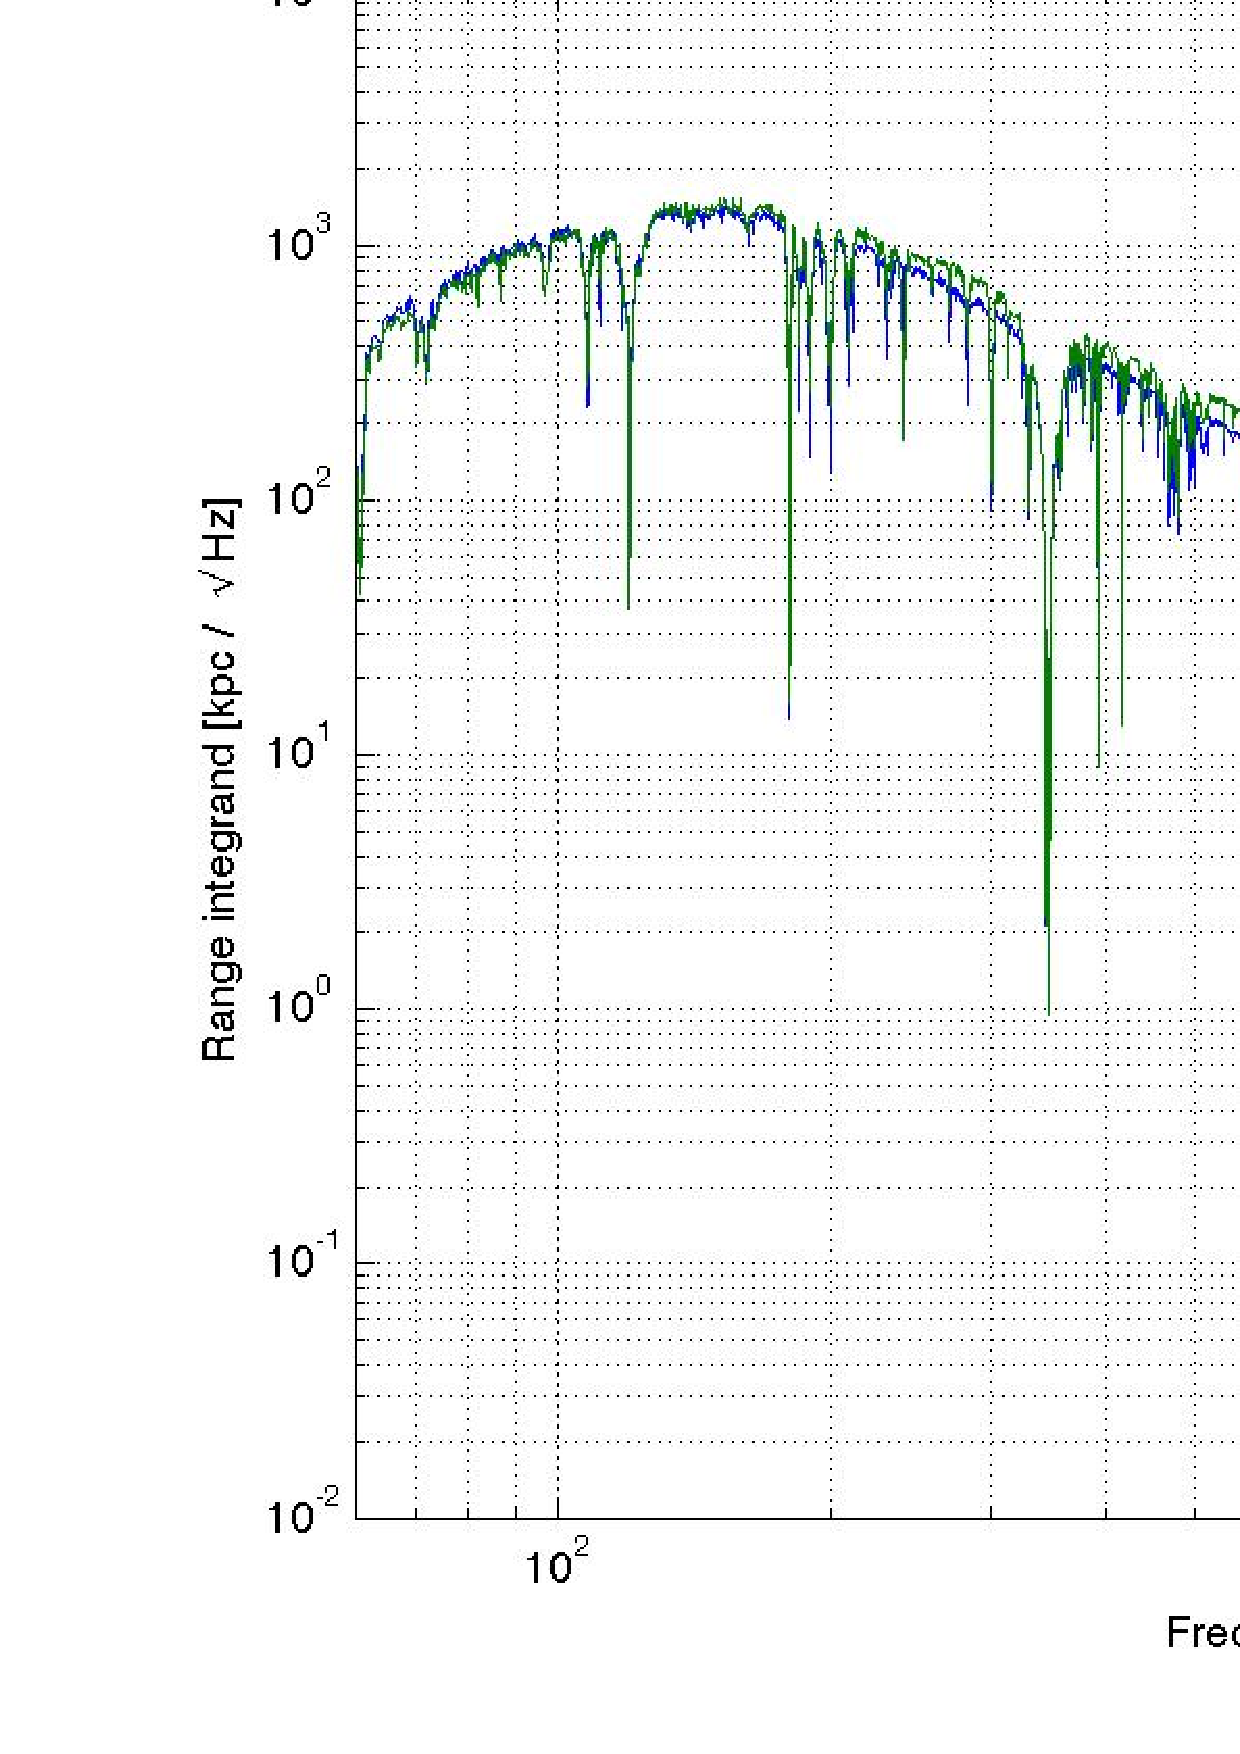
\includegraphics[width=0.45\paperwidth,height=0.45\paperheight,keepaspectratio]{range_integrand.jpeg}\protect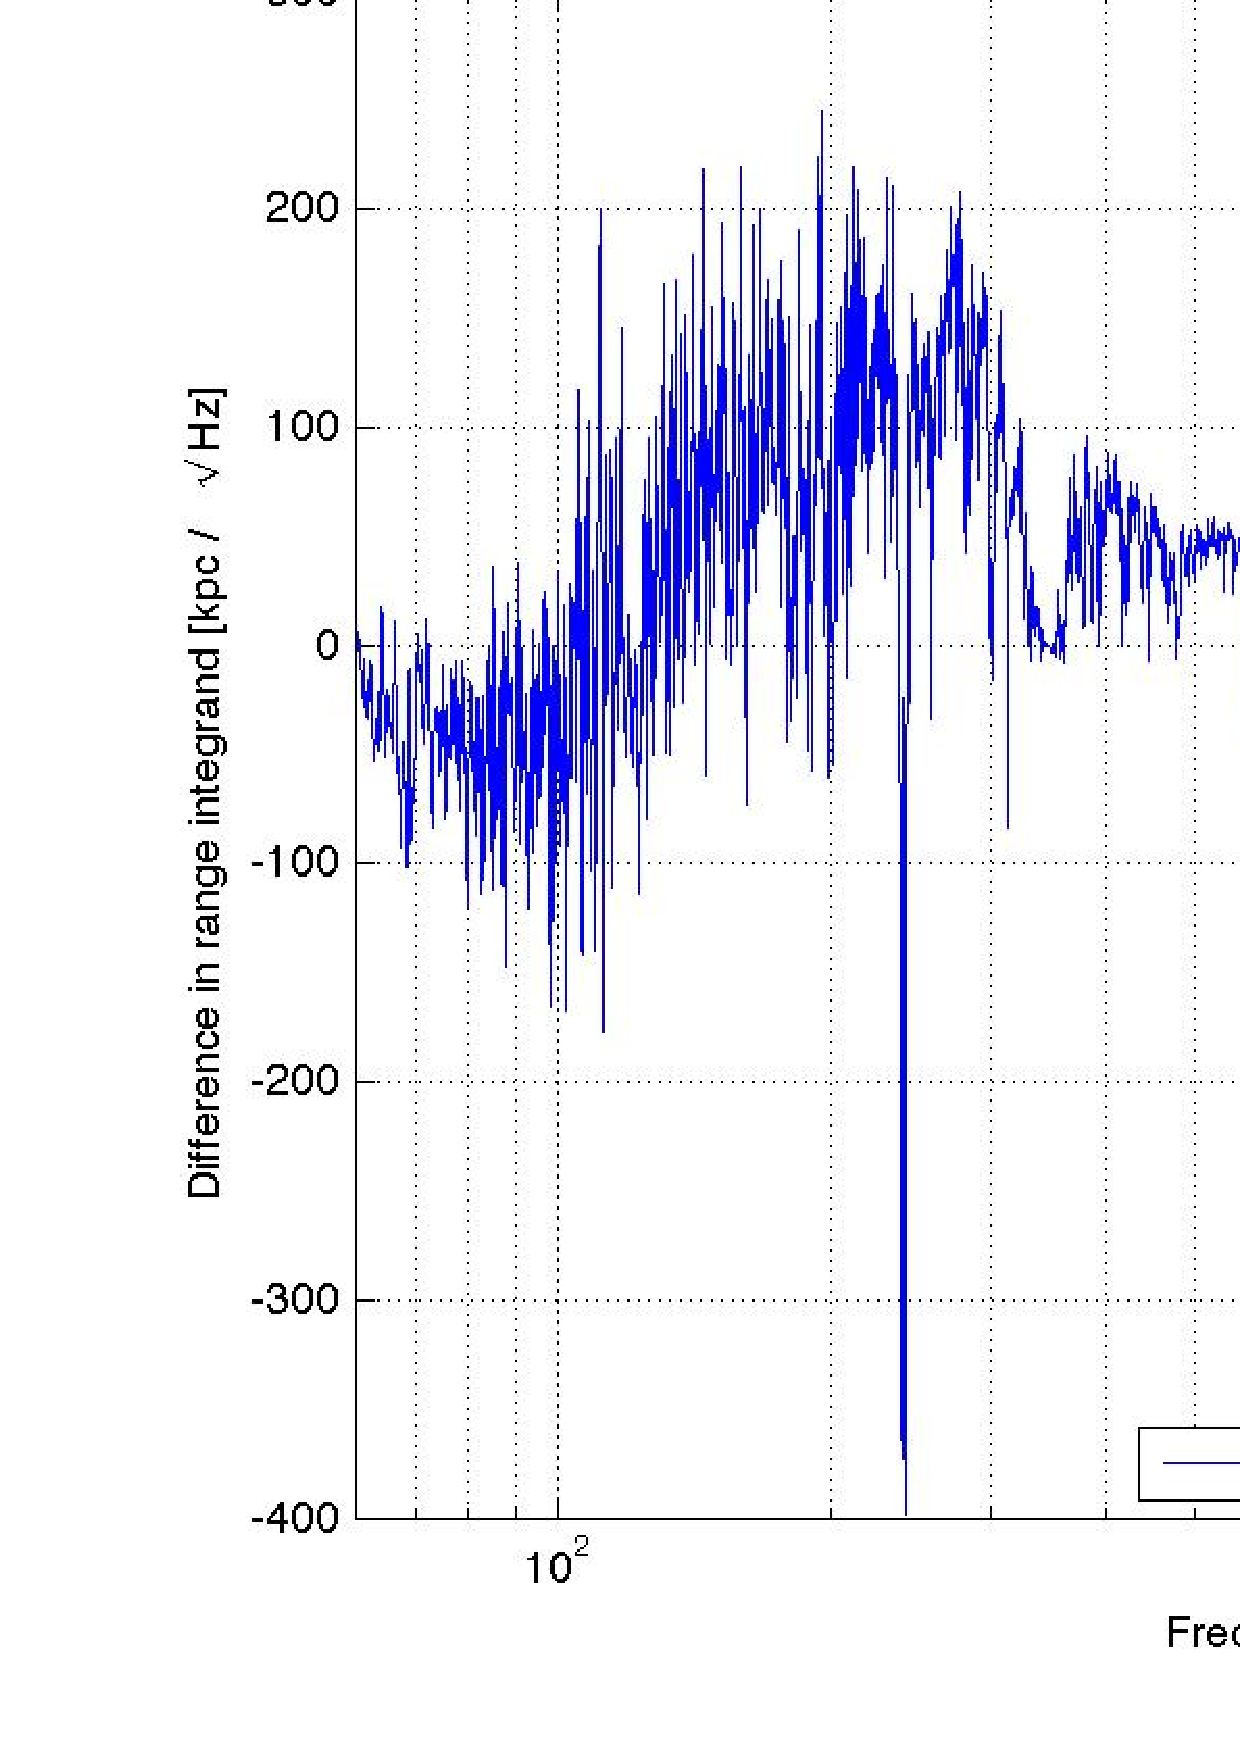
\includegraphics[width=0.45\paperwidth,height=0.45\paperheight,keepaspectratio]{range_integrand_difference.jpeg}}
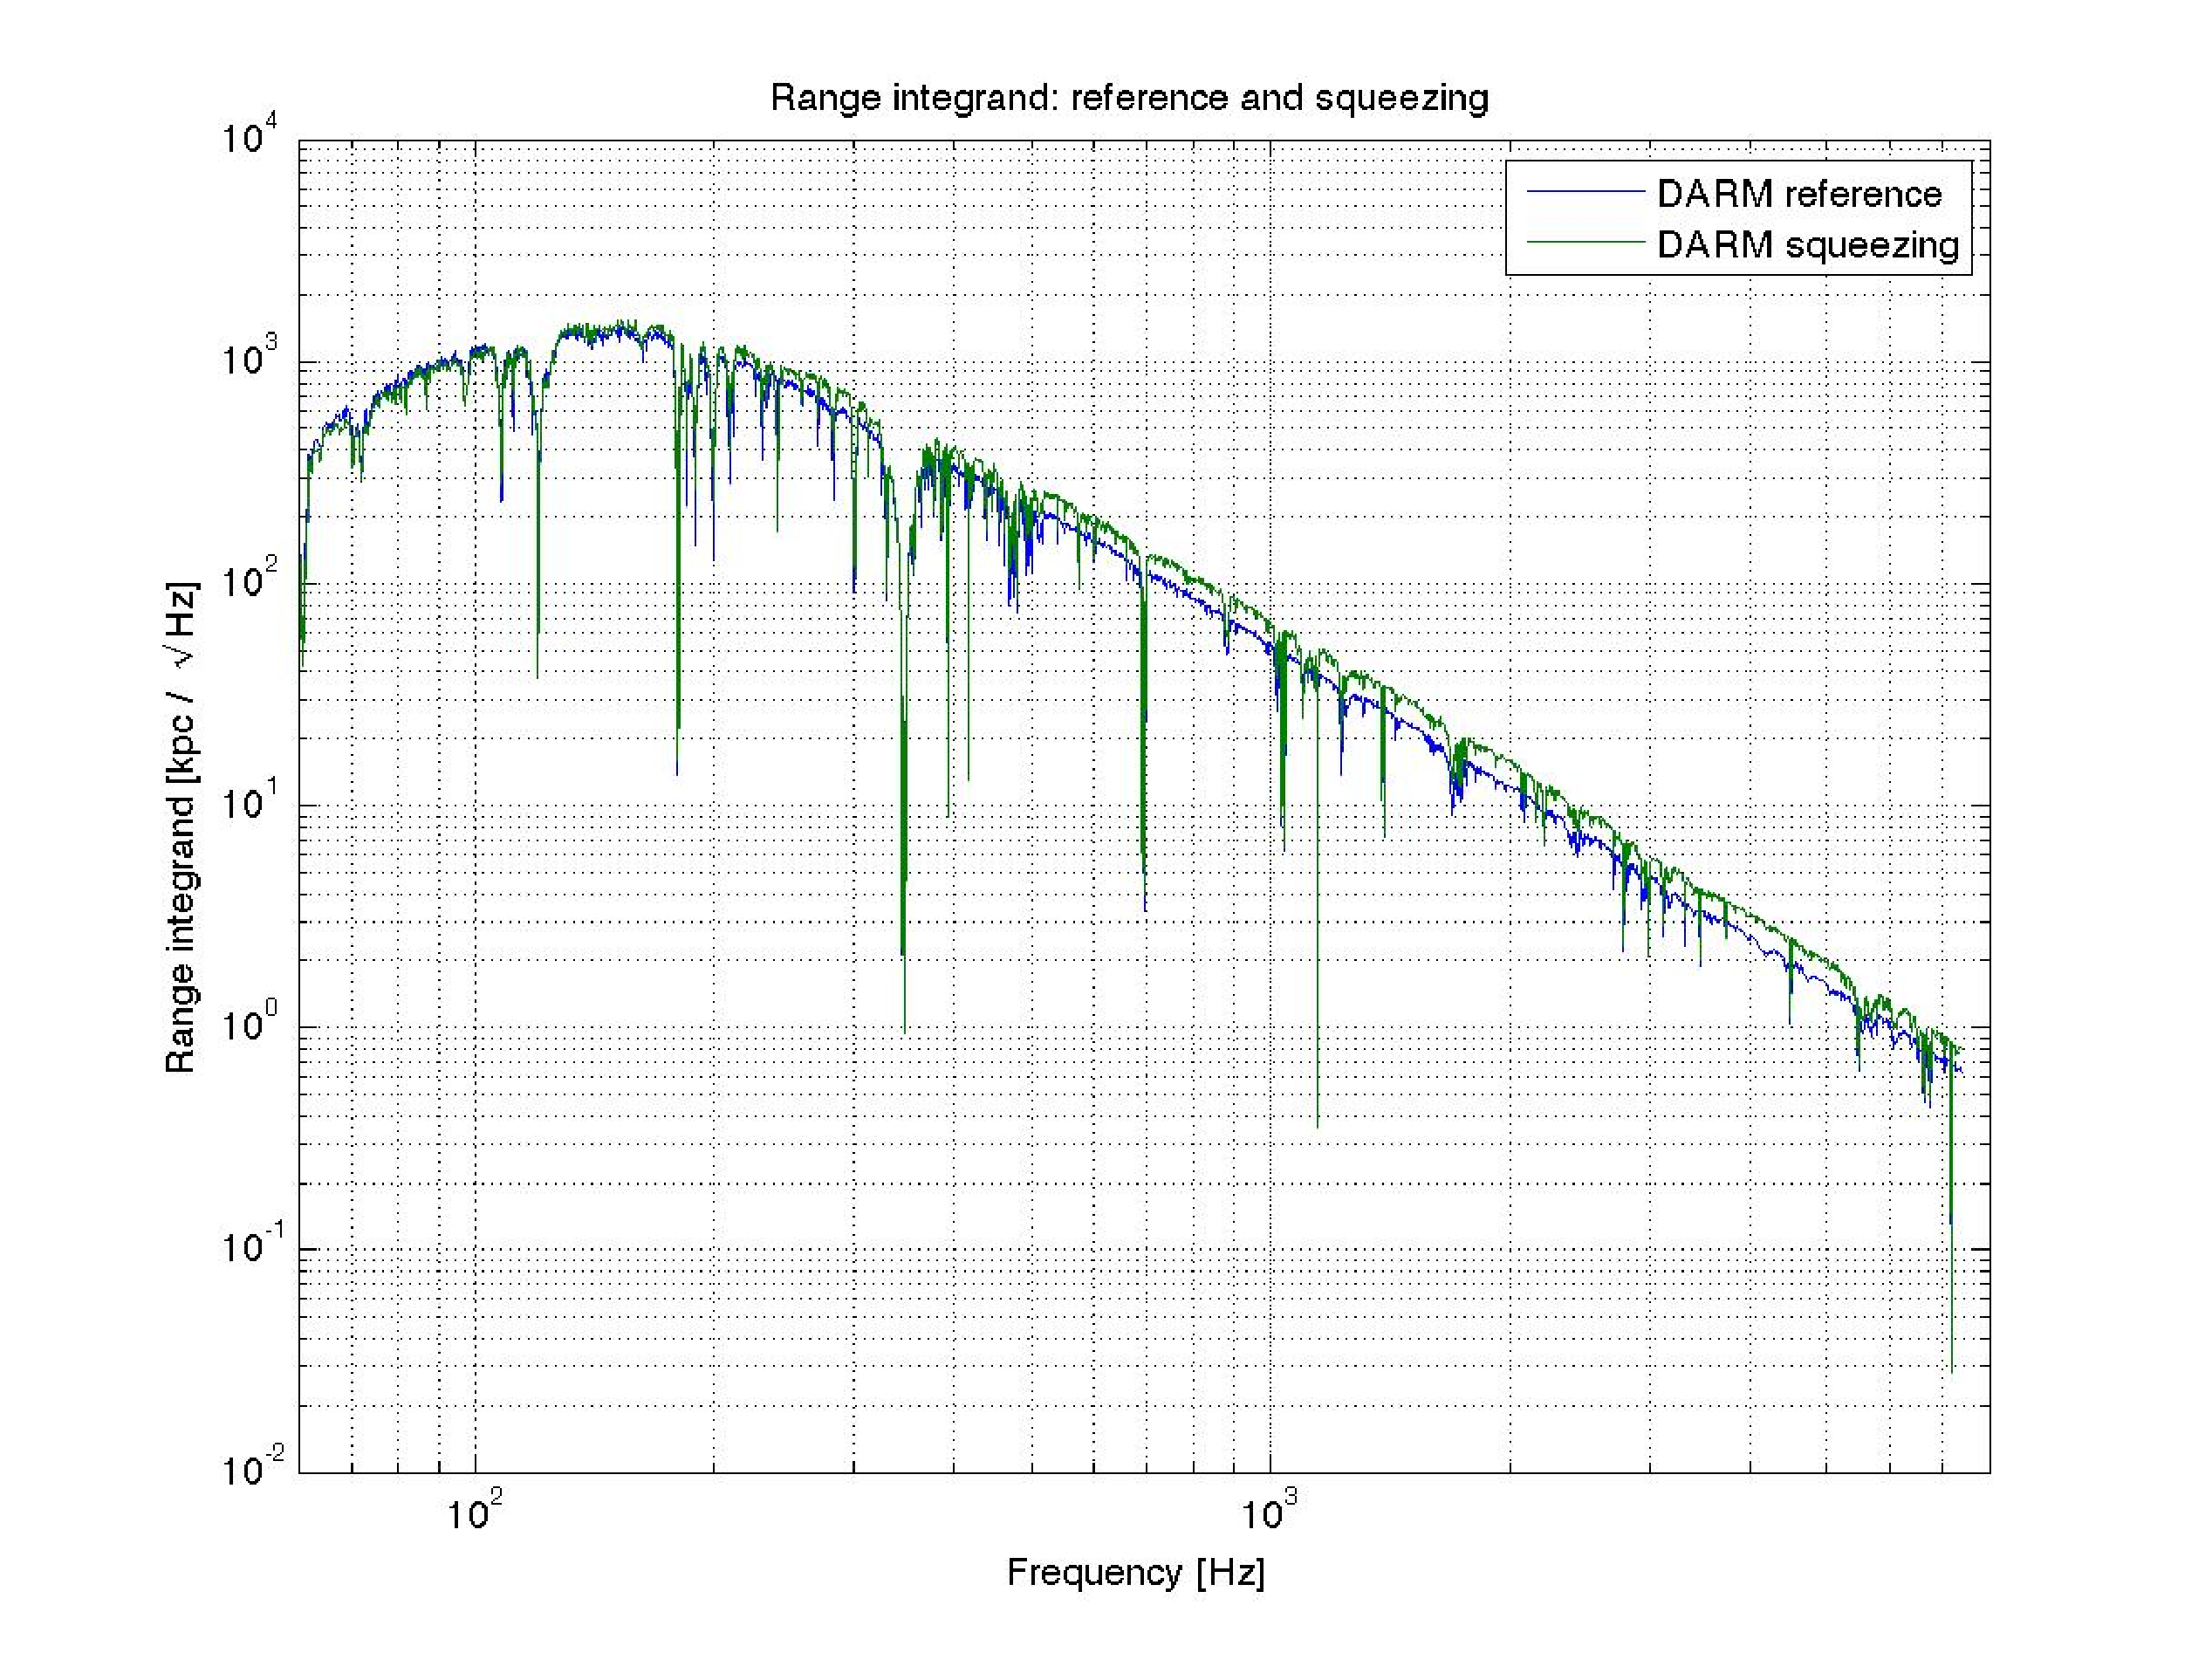
\includegraphics[height=0.5\paperheight, width=0.5\paperwidth,keepaspectratio]{range_integrand.eps}
\caption{Integrand of inspiral range as a function of frequency}
\end{figure}
\begin{figure}
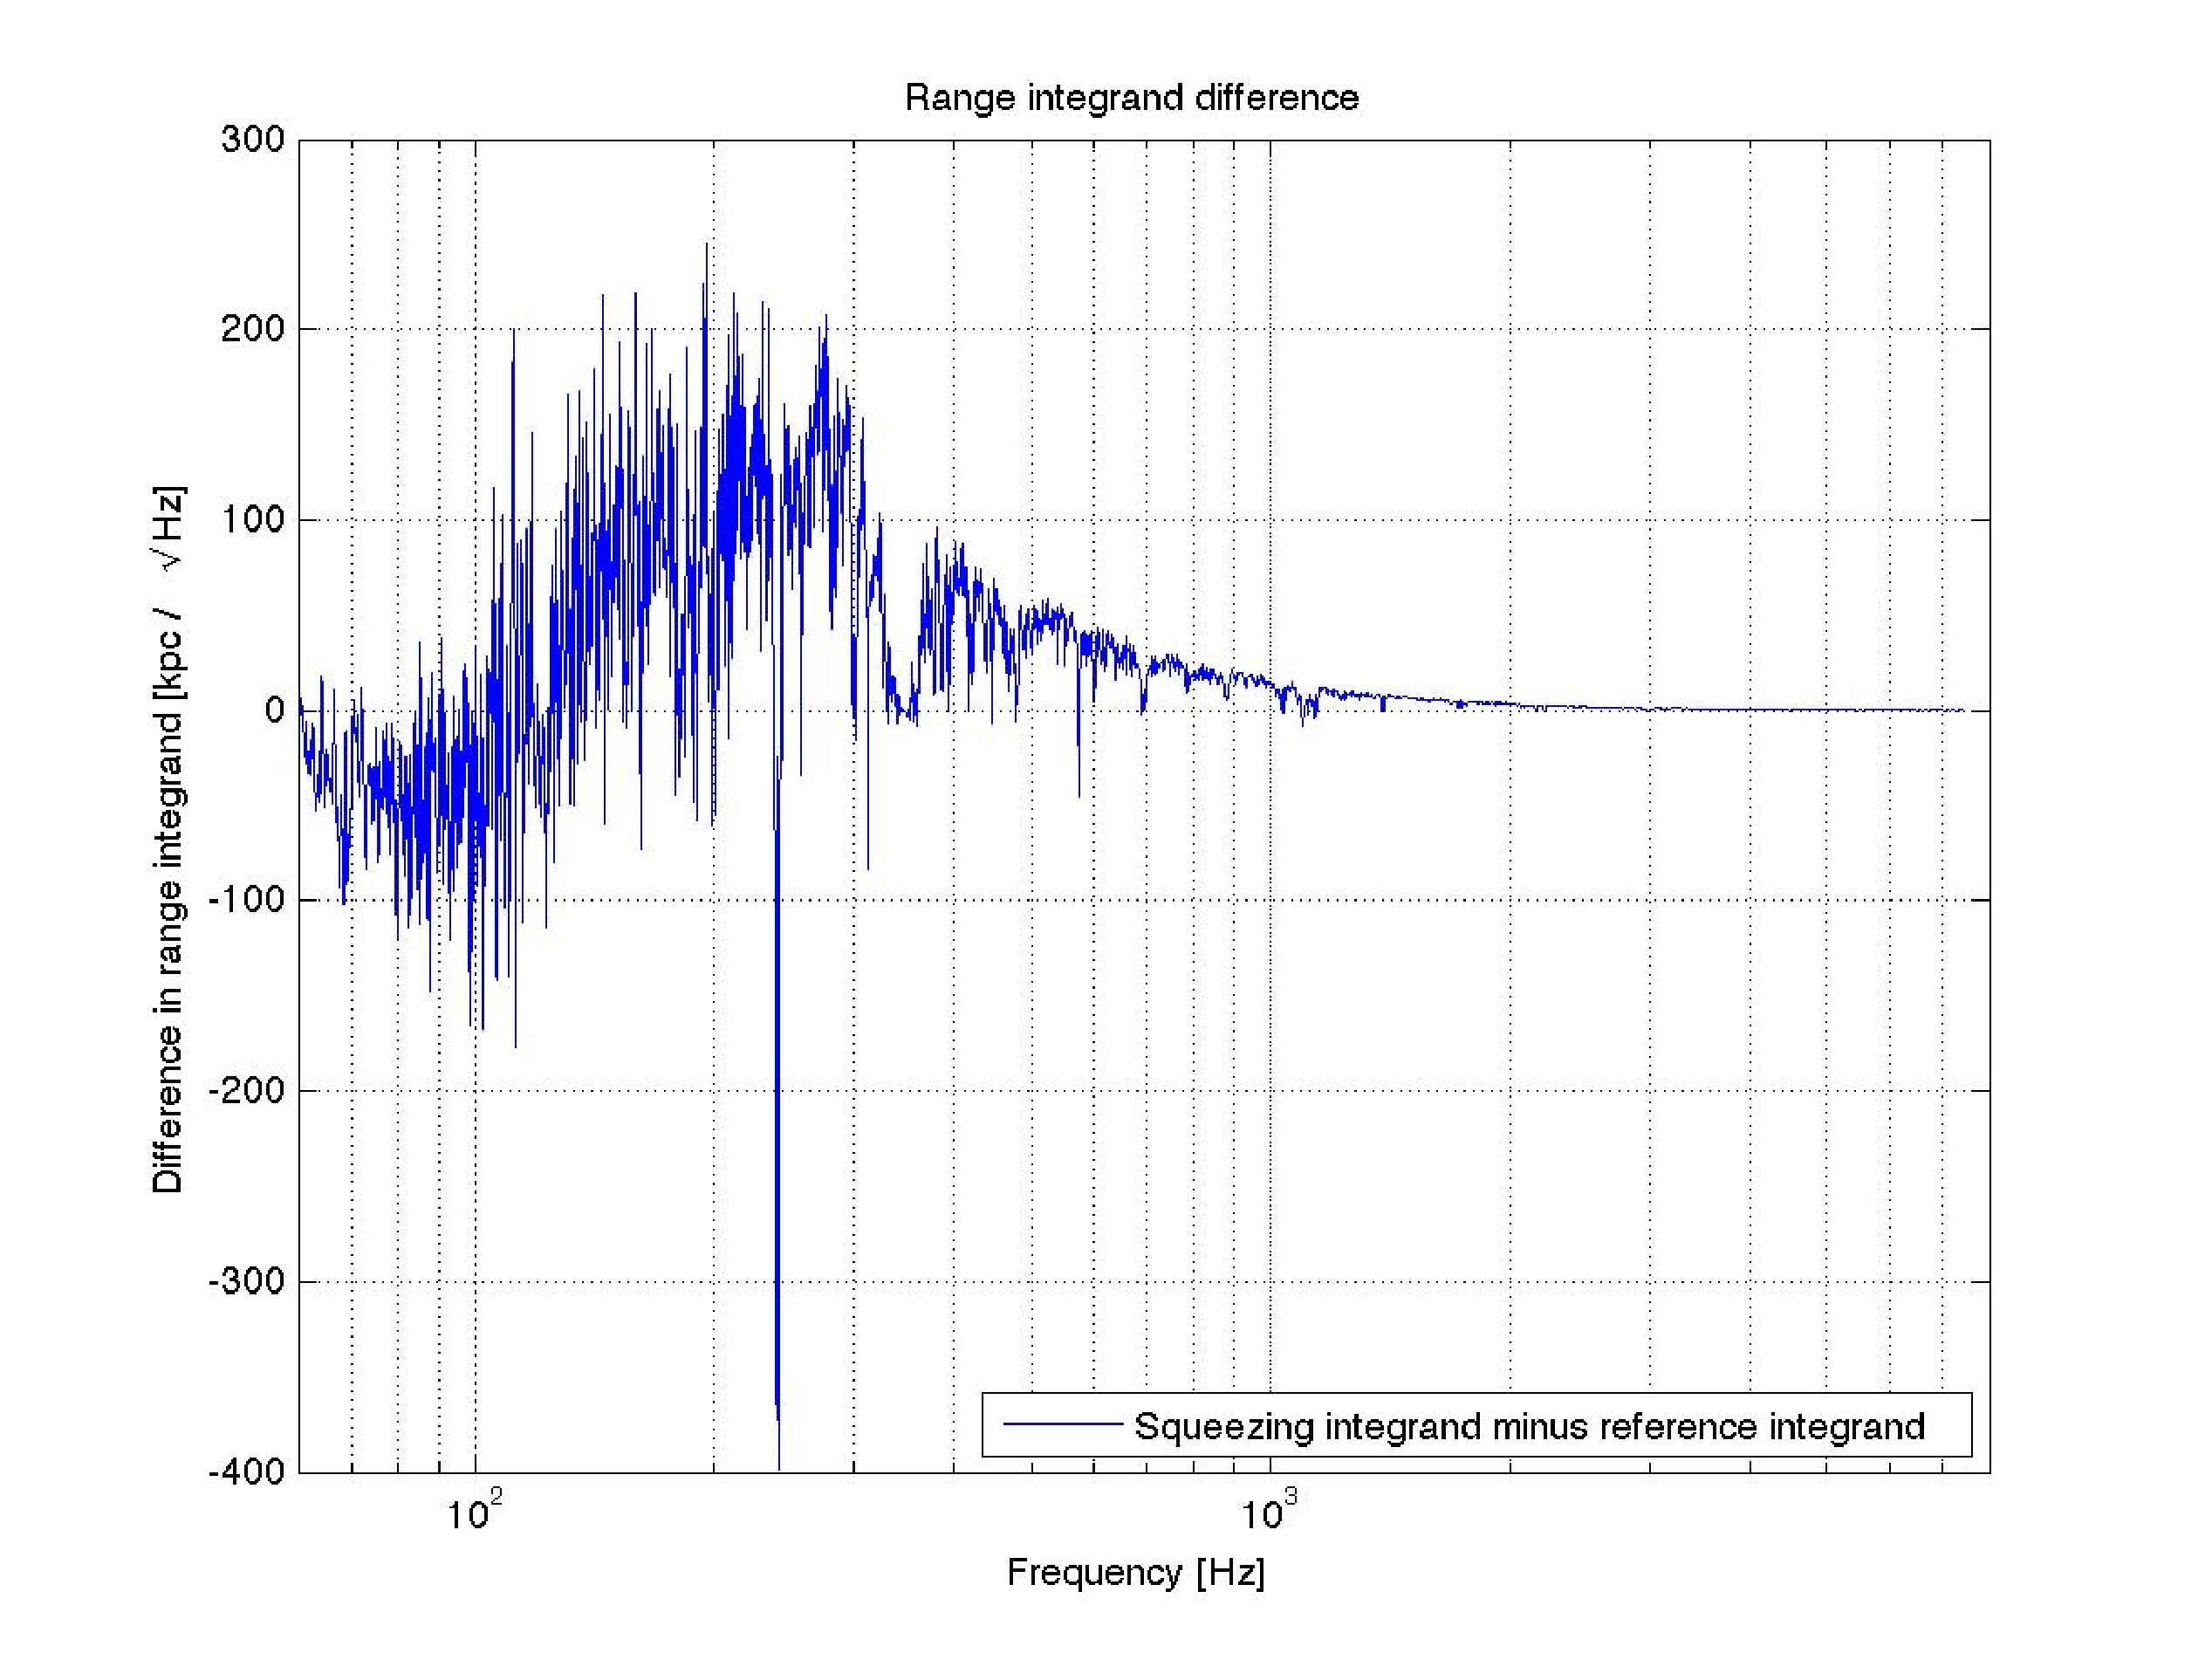
\includegraphics[height=0.5\paperheight, width=0.5\paperwidth,keepaspectratio]{range_integrand_difference.eps}
\caption{Net effect of squeezing on inspiral range integrand
\newline Scientific benefit at few hundred Hz $\rightarrow$ all ways to improve are good
}
\end{figure}




            \subsubsection{Figures of merit: inspiral range}
            \label{range_est}

                Range estimation after squeezing

		From the improved shot noise, we can see that squeezing at high frequencies bought enhanced LIGO a megaparsec of inspiral range. This number is impressive in several respects: our goal was to acheive a squeezing factor of perhaps as much as 3 dB, but to do it in the shot noise-limited region, at high frequencies, where the inspiral range equations (MATH: add the inspiral range equation if not already shown for feedforward!) count for much less. Morever, that range figure reflects the acheivement of squeezing down to 150 Hz (CITE: can we use this number?), which is the lowest yet achieved for a gravitational wave interferometer.


\section{Squeezing large interferometers}

        \subsection{Success and Advanced LIGO prospects}
        \label{squeezing_success}
            Results and hopes for aLIGO+ squeezing.

	    The squeezer group has a paper pending in review for Nature, written by Lisa Barsotti, in which we discuss our acheivement of perhaps 2 dB worth of squeezing (need to cite and check whether it is OK to use this number)~\cite{BarsottiNatureSqueezing}. It builds on the previous success of GEO600 in squeezing~\cite{GEO600NatureSqueezing}.

	    Discuss Sheila Dwyer's~\cite{DwyerPhaseNoise} and Sheon Chua's~\cite{ChuaBackscatteredLight} papers, since I am an author on both of them. We have a preliminary understanding now of at least two major problems: the quadrature phase noise fluctatuations and backscattered light. Backscattered light can be resolved in several ways. Phase noise must be progressively improved, as Sheila discusses, because we can hope to acheive the mature filter cavity design proposed below.

Discuss Lisa Barsotti's talk about the future prospect for LIGO using filter cavities, work that Tomoki Isogai is doing. With filter cavities, we can acheive frequency-dependent squeezing, having the best of both works by reducing quantum radiation pressure noise at low frequencies and shot noise at high, by using the filter cavity to produce a squeezed vacuum with a squeeze angle that varies as a function of frequency. Though as yet this filter cavity has yet to be constructed, it is in the works at MIT.

% Everything below is imported from my AEI talk




%\end{frame}

%\begin{frame}{Squeezing summary}
\subsection{Squeezing summary}

\begin{description}
\item [{Instrumental}] experience with technique important beyond Advanced
LIGO
\item [{Physical}] way to improve broad band of LIGO, benefit many searches
\item [{Illustrates}] need for best sensitivity at few hundred Hz
\item [{Question}] what can we improve \emph{post-facto?}
\end{description}
%\end{frame}


%        -------------------------------- 
%
%	The following is an example of using the commands \textit{ref}
%	and \textit{label}. With these commands theorems, chapters,
%	sections and figurres can be labeld with names in the tex file
%	and then refered to by these names in later tex files. In
%	chapter~\ref{intro} we saw section~\ref{sample_section} or
%	theorem~\ref{sample_theorem}.
%
%	Lastly, here is how to include a figure. First generate an
%	encapsulated postscript file in xfig, adobe illustrator or
%	some other program. The specific commands are found in
%	\textit{chap2.tex}.
%
%        \begin{figure}[htb]
%        \centerline{ \epsfig{figure=sample.eps, 
%        height =  1.5 in}}
%        \caption{Sample Figure}
%        \label{sample_figure}
%        \end{figure}


% Squeezing contributions
\chapter{TwoSpect: Binary Pulsar Searches}
\label{chap4}


    %(Fill in bits about the squeezer)

Gravitational wave interferometry measures changes in light travel time far less than the light-crossing time of an atom, so the quantum nature of light has always influenced detector design.
Advanced LIGO aims to resolve most of noise sources described in Sections~\ref{methods} and~\ref{interferometer_theory}: even so, quantum shot and radiation pressure noise from light will remain.
Carlton Caves correctly derived the quantum behavior of interferometer shot and radiation pressure noise~\cite{Caves1980}.
Prior work had inferred the shot noise level from classical principles, accurately, but been ambiguous about radiation pressure.
With the quantum noise clarified, it was realized that this noise could be reduced through so-called squeezing of the vacuum state~\cite{Caves1981}.
This chapter describes part of how squeezing was successfully realized three decades later at the LIGO Hanford Observatory.
For additional details, consult Chua~\cite{ChuaThesis} and Dwyer~\cite{DwyerThesis}.

    \section{Squeezing theory}
    \label{squeezing_theory}

        Squeezing theory.

        \subsection{Quantum shot noise and radiation pressure}
        \label{quantum_noise}

            %Carlton Caves, quantum shot noise and radiation pressure.

%\begin{frame}{Squeezing introduction}

%\begin{definition}
Altering $\Delta E\Delta\phi$ uncertainty for the electromagnetic
field
%\end{definition}
\begin{itemize}
\item Demonstrated first at GEO 600, then LIGO Hanford (H1)\end{itemize}
\begin{theorem}
Shot noise arises from quantum operators (Caves 1980, 1981)\end{theorem}
\begin{itemize}
\item Vacuum fluctuations couple through anti-symmetric port
\item \emph{Squeeze }the $\overrightarrow{E}$ field uncertainty ellipse
\item Angle $\theta$, factor $r$, creation operator $a$, squeeze operator
$S$:
\end{itemize}

From the Caves squeezing paper~\cite{Caves1981},

\[
S(\zeta)=\exp[\frac{1}{2}\zeta^{*}a^{2}-\frac{1}{2}\zeta(a^{\dagger})^{2}],\;\zeta=re^{i\theta}
\]



Squeezed state made with


optical parameter oscillator, 2nd harmonic generator


\textbf{Shot noise reduced by $e^{-r}$}


\[
\]




        \subsection{Problems with lasers: thermal compensation}
        \label{TCS}

            Experience (some firsthand) with thermal compensation.

        \subsection{Squeezing filter cavities against alternatives}
        \label{third-gen_squeezing}

    \section{LIGO Hanford Observatory quantum vacuum squeezing}
    \label{LHO_squeeze}

        Quantum vacuum squeezing at LIGO Hanford Observatory. Naturally, a great deal of description and background will come from Sheila Dwyer's thesis~\cite{DwyerThesis} and Sheon Chua's thesis~\cite{ChuaThesis}.

        \subsection{Collaboration and contributions}
        \label{contributions}

            Contributions: table, in-vacuum installation, electronics, range est.

            \subsubsection{Optical table support assembly}
            \label{table_legs}

                Table legs (me) and results of Sheon and Robert's shakers.

		Here might be good place to put old AutoCAD drawings to use.
\begin{figure}
\begin{center}
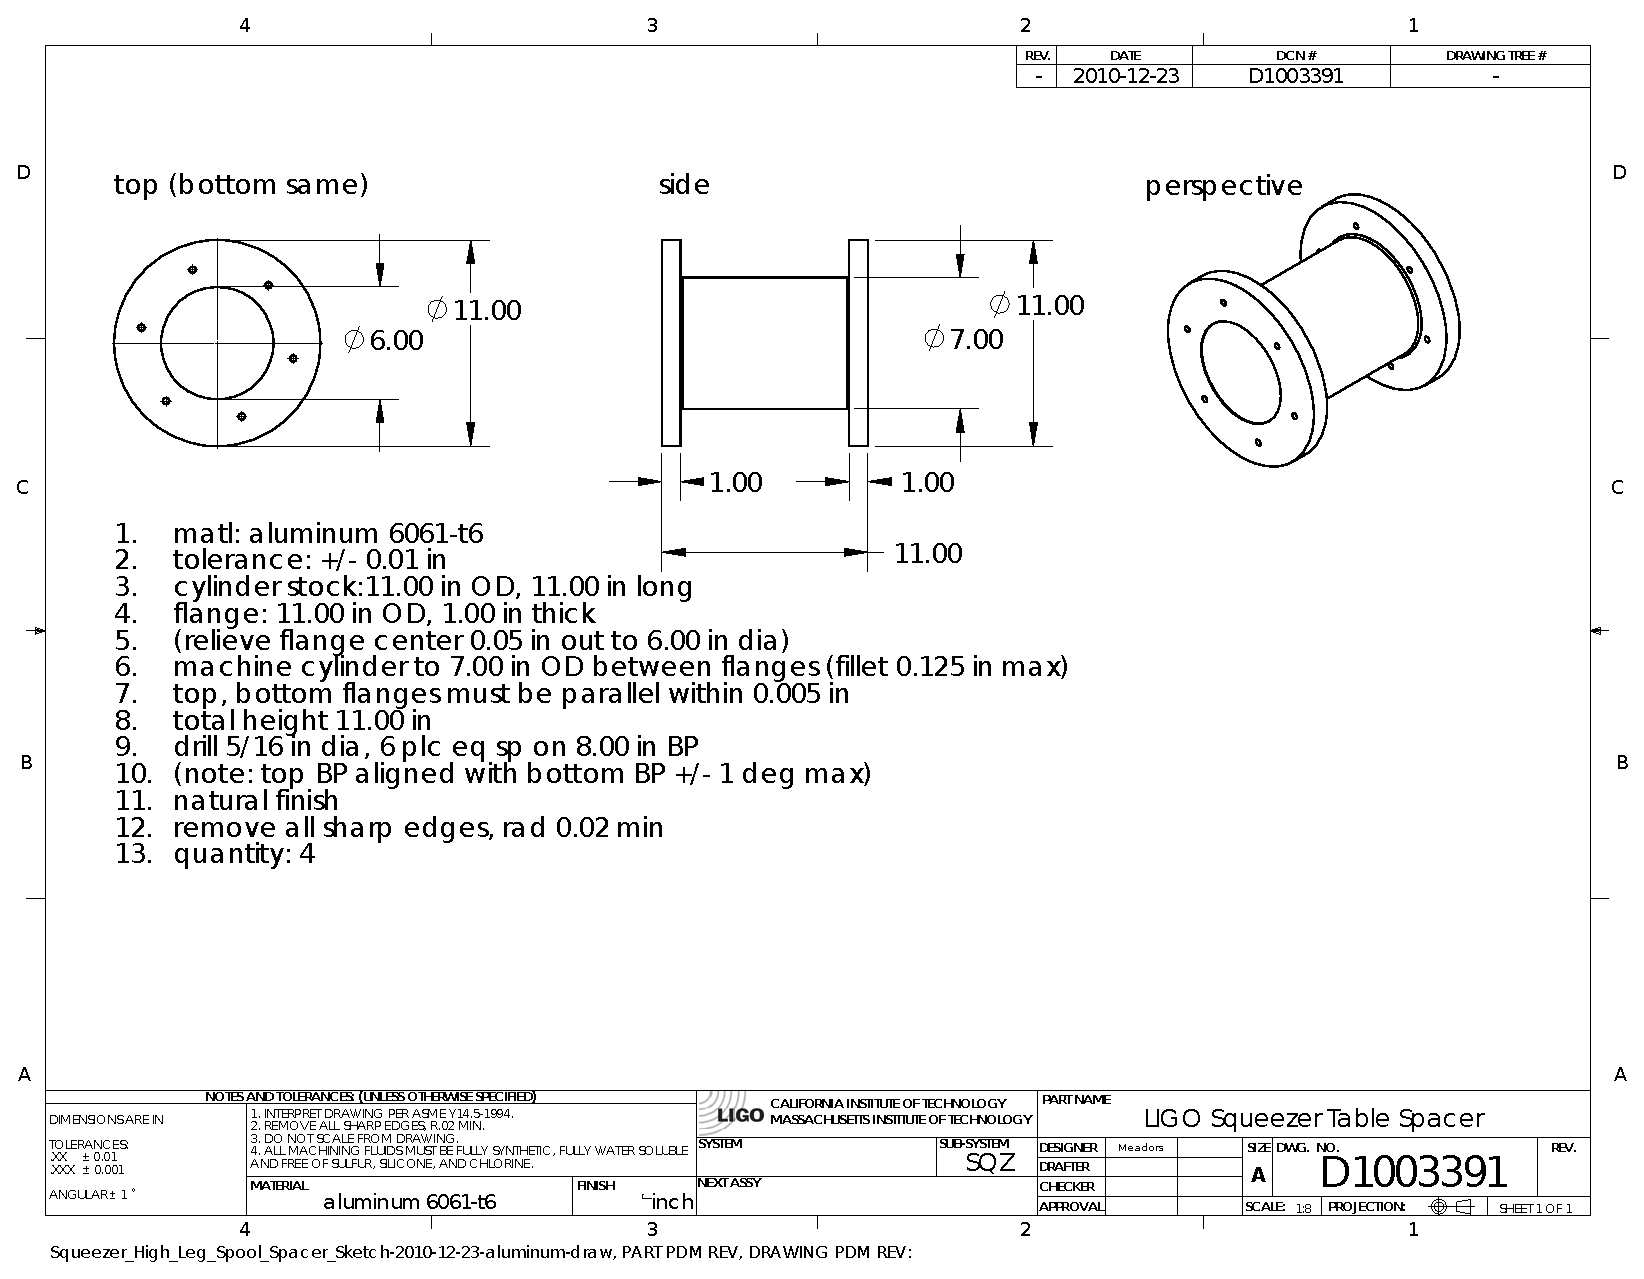
\includegraphics[width=0.6\paperwidth]{Squeezer_High_Leg_Spool_Spacer_2010-12-23_aluminum.eps}
\caption{Table legs SolidWorks schematic. This initial design for the table leg extensions on the squeezer table incorporated a flange, which was removed immediately prior to fabrication, replaced with a larger diameter flangeless tube with incorporated tap-holes. Flanges were thought necessary for a flexible alignment initially, they would be prohibitively expensive to machine, and welding would induce unacceptable distortions into the metal. Design in consultation with Daniel Sigg, Lisa Barsotti, Keita Kawabe, Gerardo Moreno, Richard Savage.
}
\end{center}
\end{figure}


            \subsubsection{Faraday isolator measurement}
            \label{Faraday}

                Faraday isolator measurements were performed by Keita Kawabe, Matt Evans, Lisa Barsotti along with myself.

		What were the results of the measurement? Show e-log entries, comment on in-and-out-of-vacuum performance and what it says about the need for low loss to be a top priority in future squeezing efforts.

            \subsubsection{In-vacuum installation}
            \label{In-vacuum}

                In-vacuum Faraday and baffle installation with "".

                Show pictures of the installation, connect to the issues with stray and perhaps backscattered light.

		Discuss the repair of the output mode cleaner, which is mentioned (citation 50) in Nic's thesis~\cite{SmithThesis}. The technical report corresponding to it is by Waldman and Chua~\cite{Waldman2011}.

            \subsubsection{Data digitization}
            \label{data_digitization}

                Electronic cabling and analog-to-digital converter installation.
                Added data channels with David Barker.

		May want helpful diagram.



%\end{frame}

%\begin{frame}{Squeezing large interferometers}


\begin{figure}
\begin{center}
%\protect\caption{\protect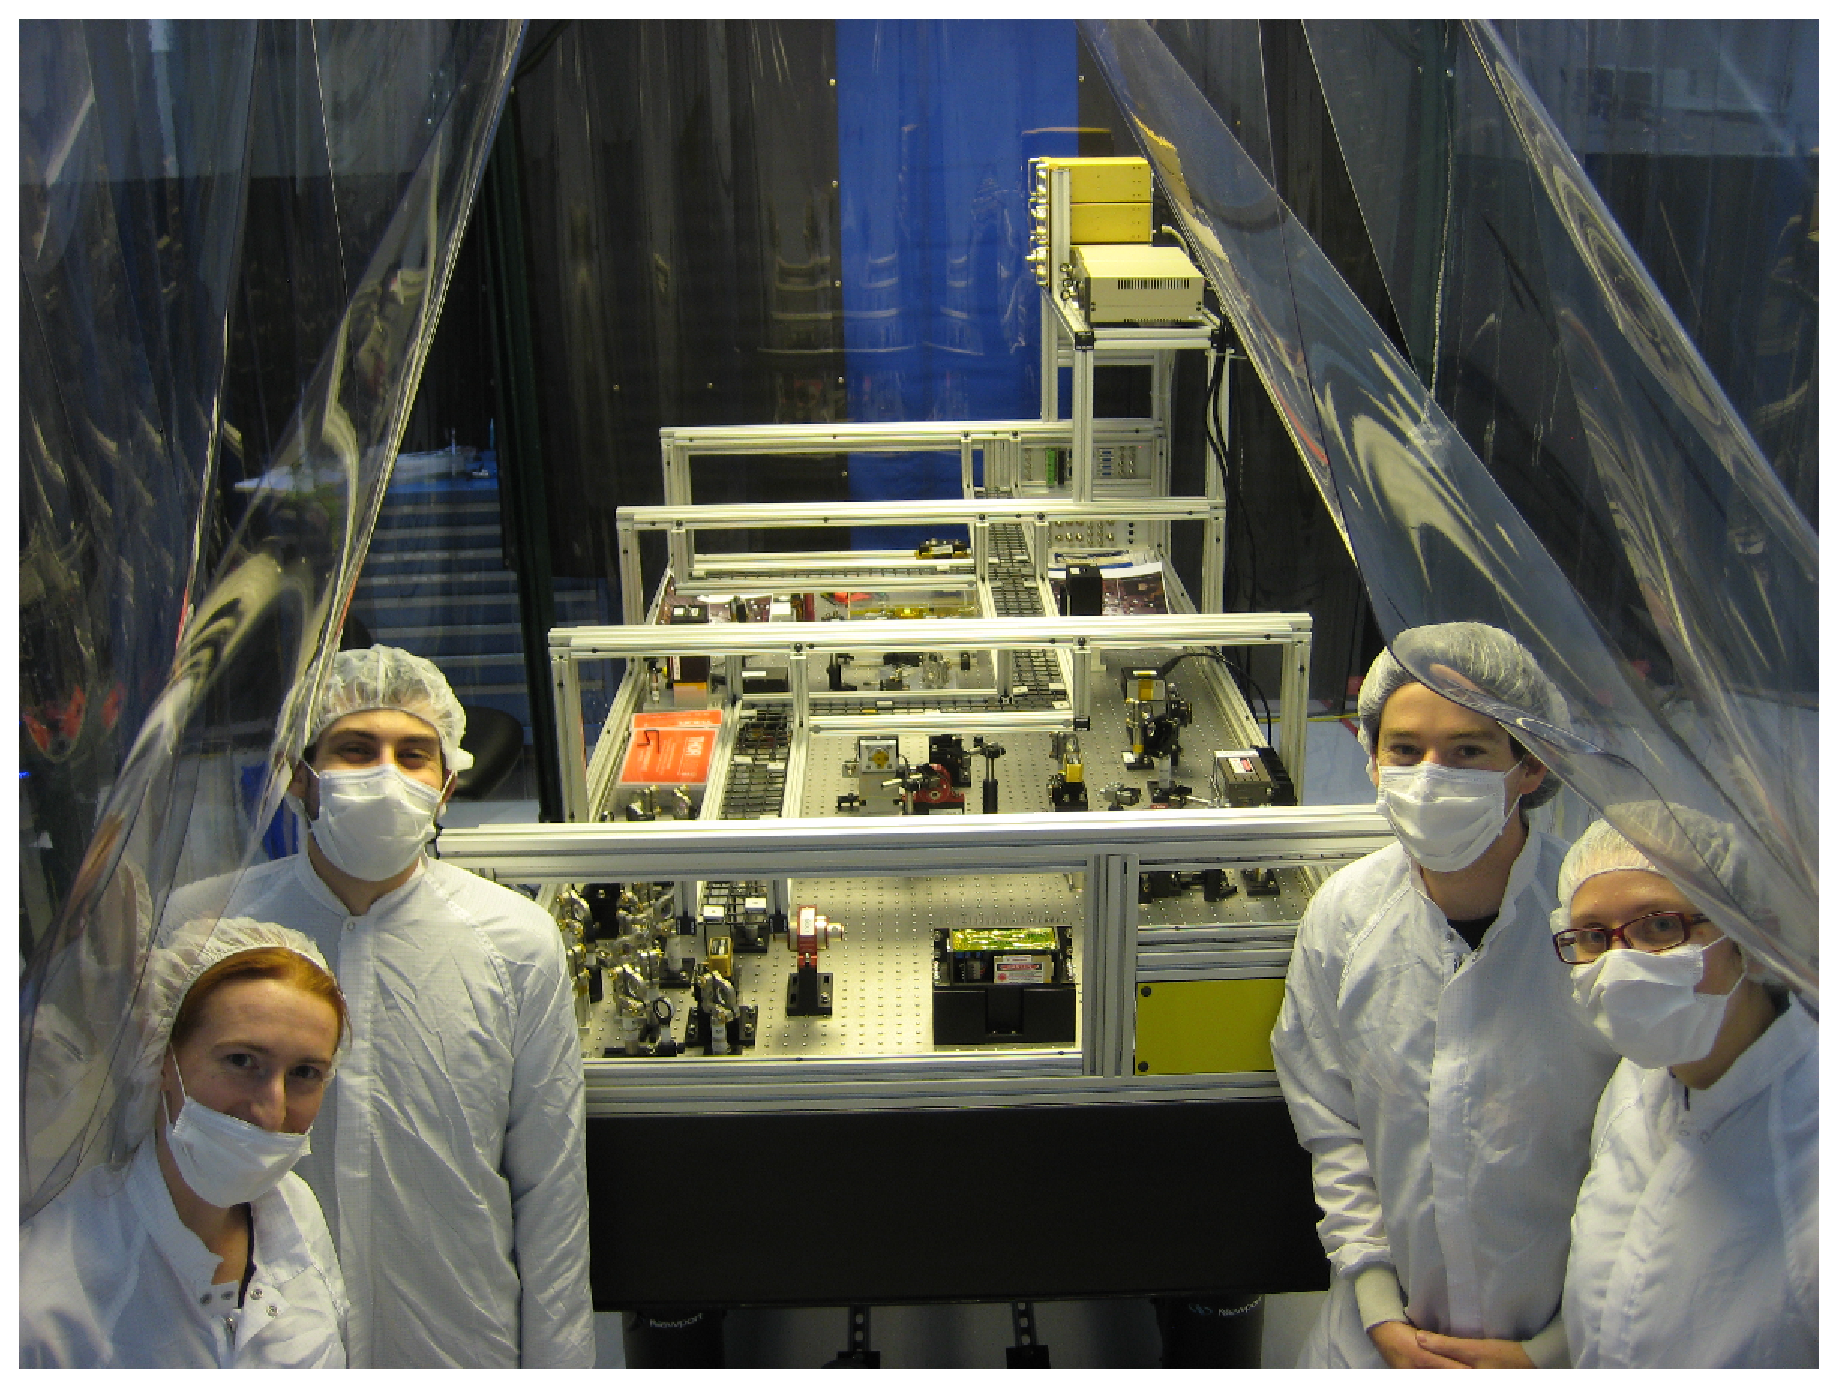
\includegraphics[width=0.33\paperwidth]{lisabar-1289966130}}
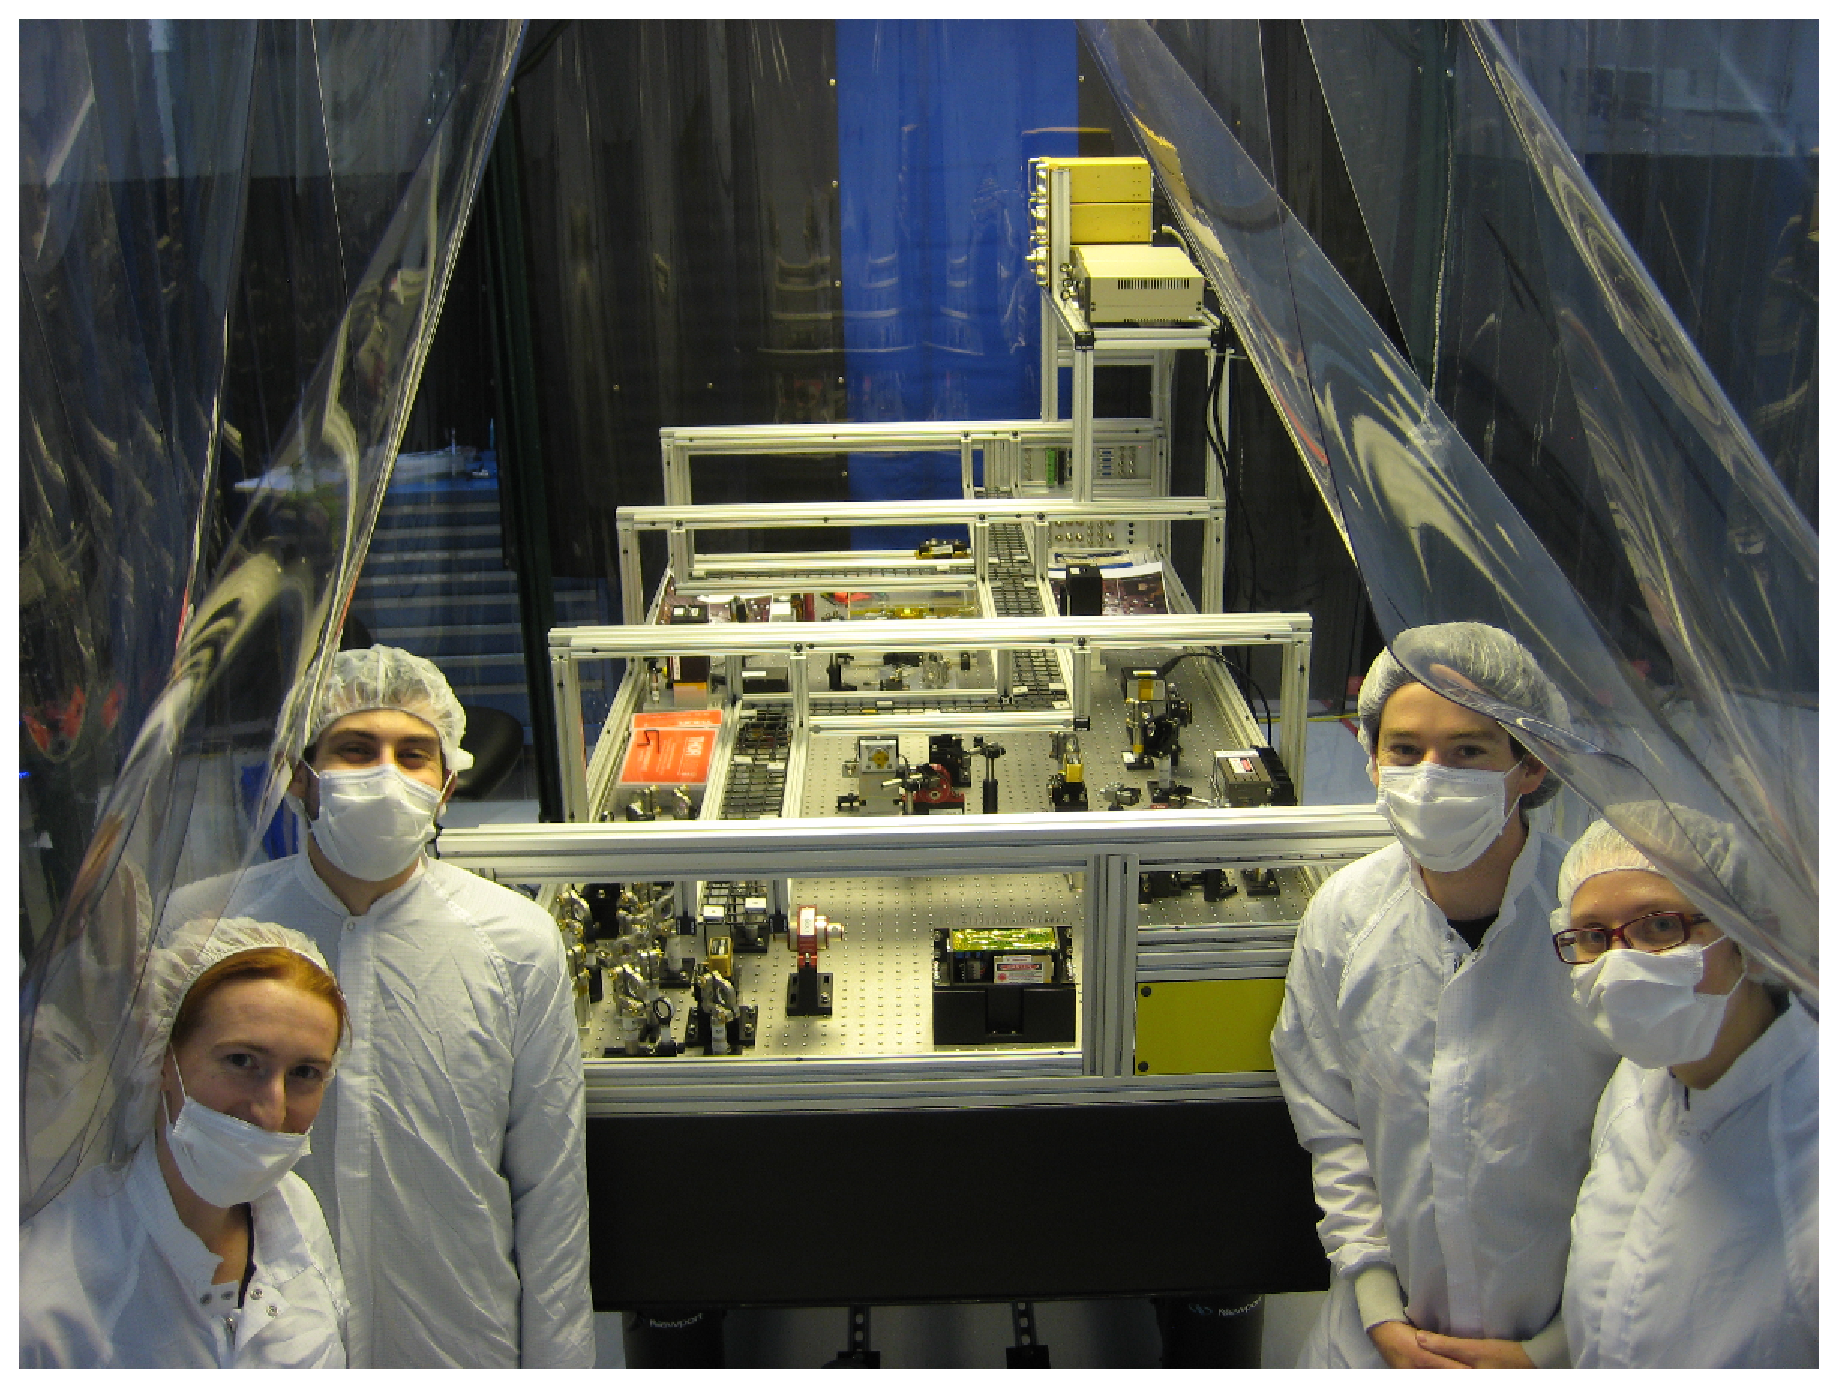
\includegraphics[width=0.6\paperwidth]{lisabar-1289966130.eps}


%\protect\caption{\protect\includegraphics[width=0.33\paperwidth]{lisabar-1300943141}}


\caption{Image by Lisa Barsotti in Hanford eLog.
\newline Counterclockise from lower left: Sheila Dwyer, Lisa Barsotti, Conor Mow-Lowry, Grant Meadors. This photograph shows the uncovered squeezer table with components from the MIT squeezer experiment unpacked at LIGO Hanford Observatory in November 2010. The table sat in a temporary location by HAM6, where it was recommissioned by Dwyer, Mow-Lowry, Sheon Chua, and Alexander Khalaidovksi until H1 could be brought back online for the squeezing experiment in late 2011. 
}
\end{center}
\end{figure}
\begin{figure}
\begin{center}
\includegraphics[width=0.6\paperwidth]{lisabar-1300943141.eps}
\caption{Table legs testing. The squeezer table is raised to its final height by the leg extensions. From top to bottom: table (WISCT10), existing leg extensions (with flanges), new leg extensions (flangeless), triangular high table legs. This assemblage provided the squeezer a serendiptously-stable (as measured by Sheila Dwyer and Robert Schoield) platform at low cost. Photo in temporary location; the actual squeezer table was anchored to these table legs, grouted, by HAM4.
}
\end{center}
\end{figure}


%\end{frame}

%\begin{frame}{Squeezing's scientific benefit}
\subsection{Squeezing's scientific benefit}


\begin{figure}
\begin{center}
%\protect\caption{\protect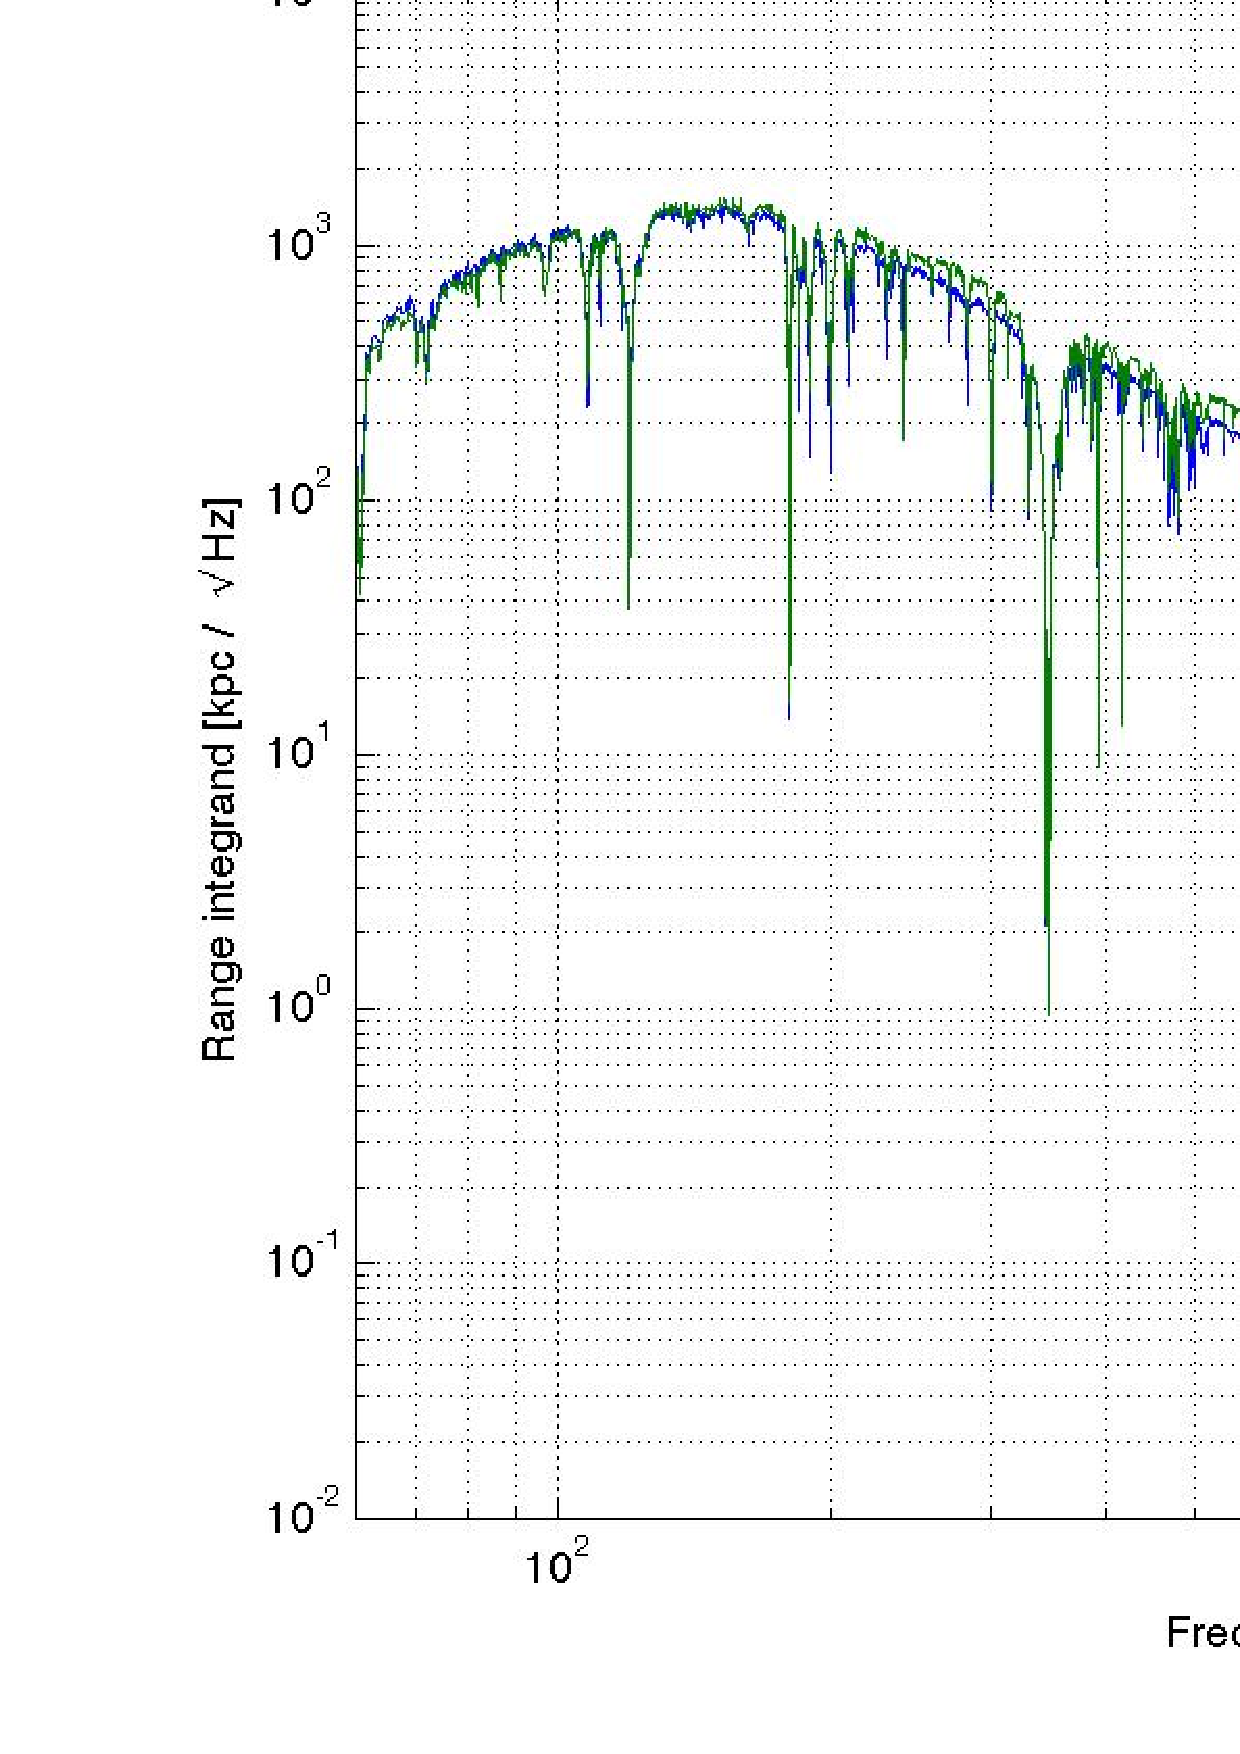
\includegraphics[width=0.45\paperwidth,height=0.45\paperheight,keepaspectratio]{range_integrand.jpeg}\protect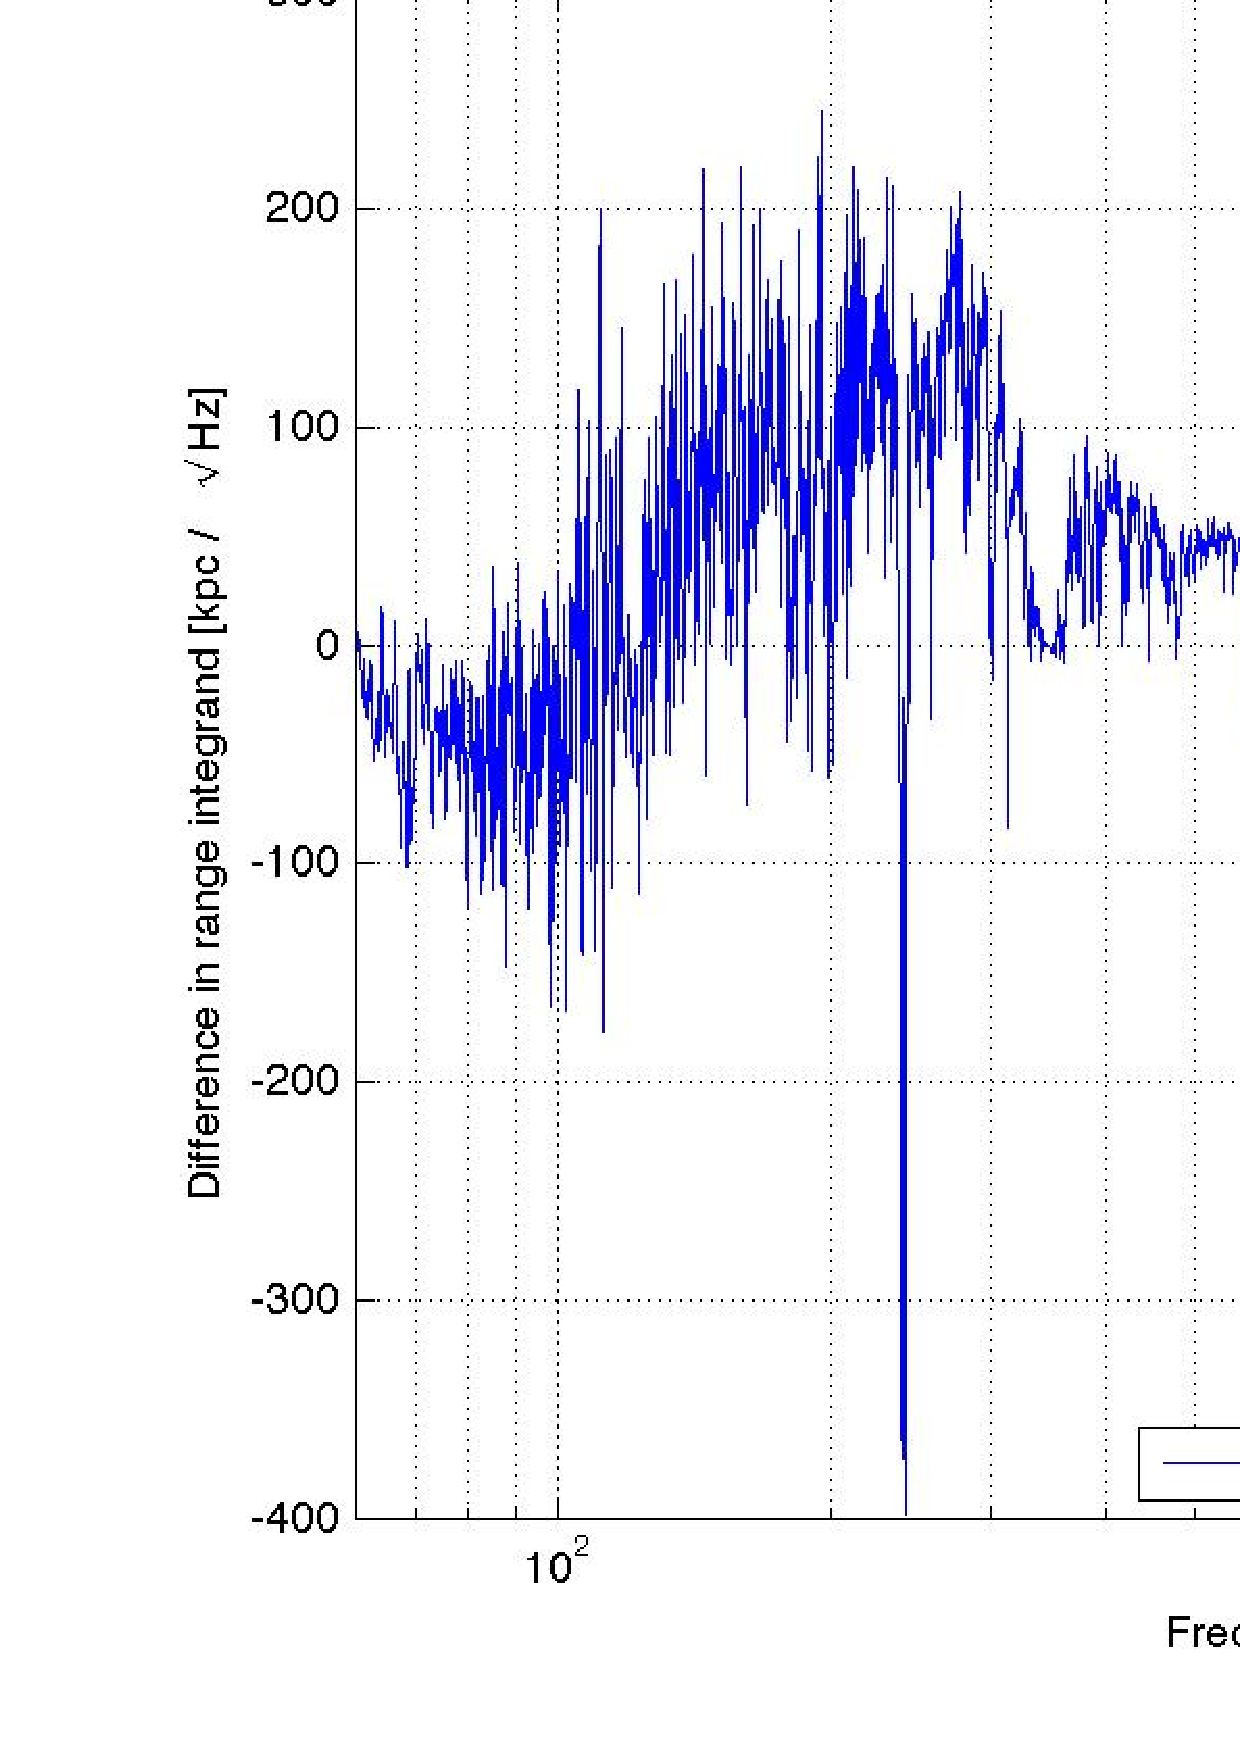
\includegraphics[width=0.45\paperwidth,height=0.45\paperheight,keepaspectratio]{range_integrand_difference.jpeg}}
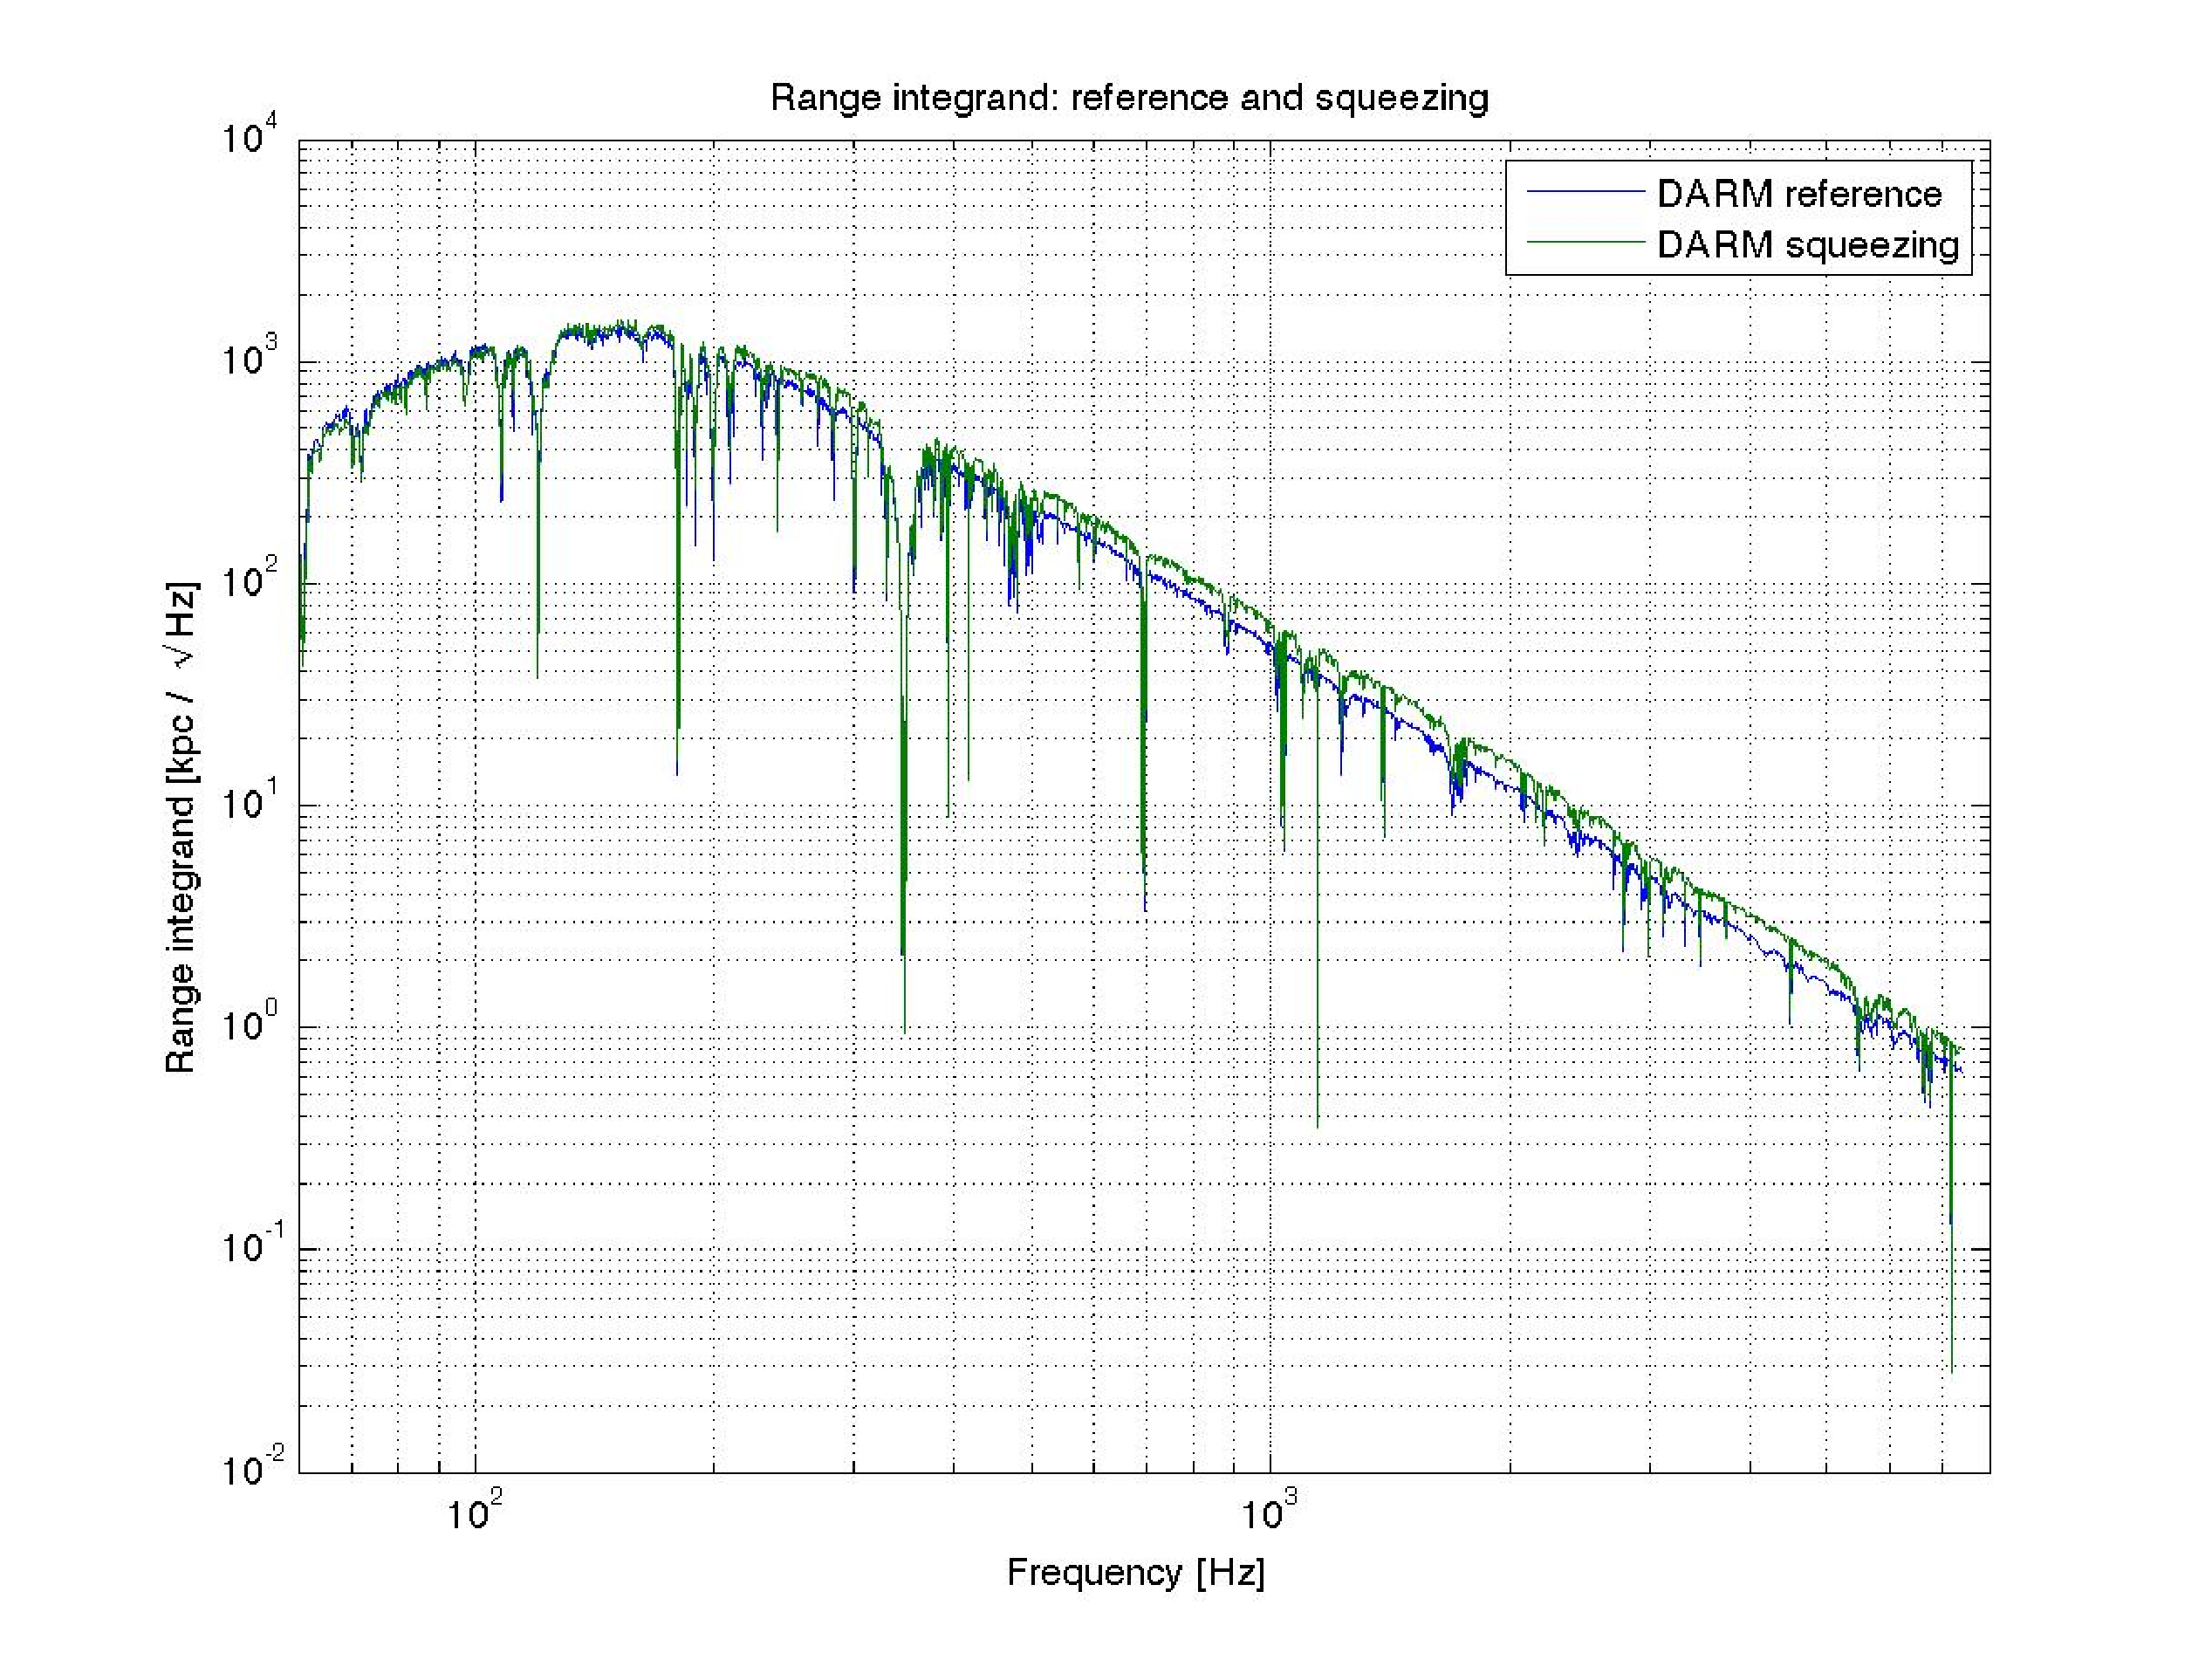
\includegraphics[height=0.5\paperheight, width=0.5\paperwidth,keepaspectratio]{range_integrand.eps}
\caption{Integrand of inspiral range as a function of frequency, with and without squeezing.}
\end{center}
\end{figure}
\begin{figure}
\begin{center}
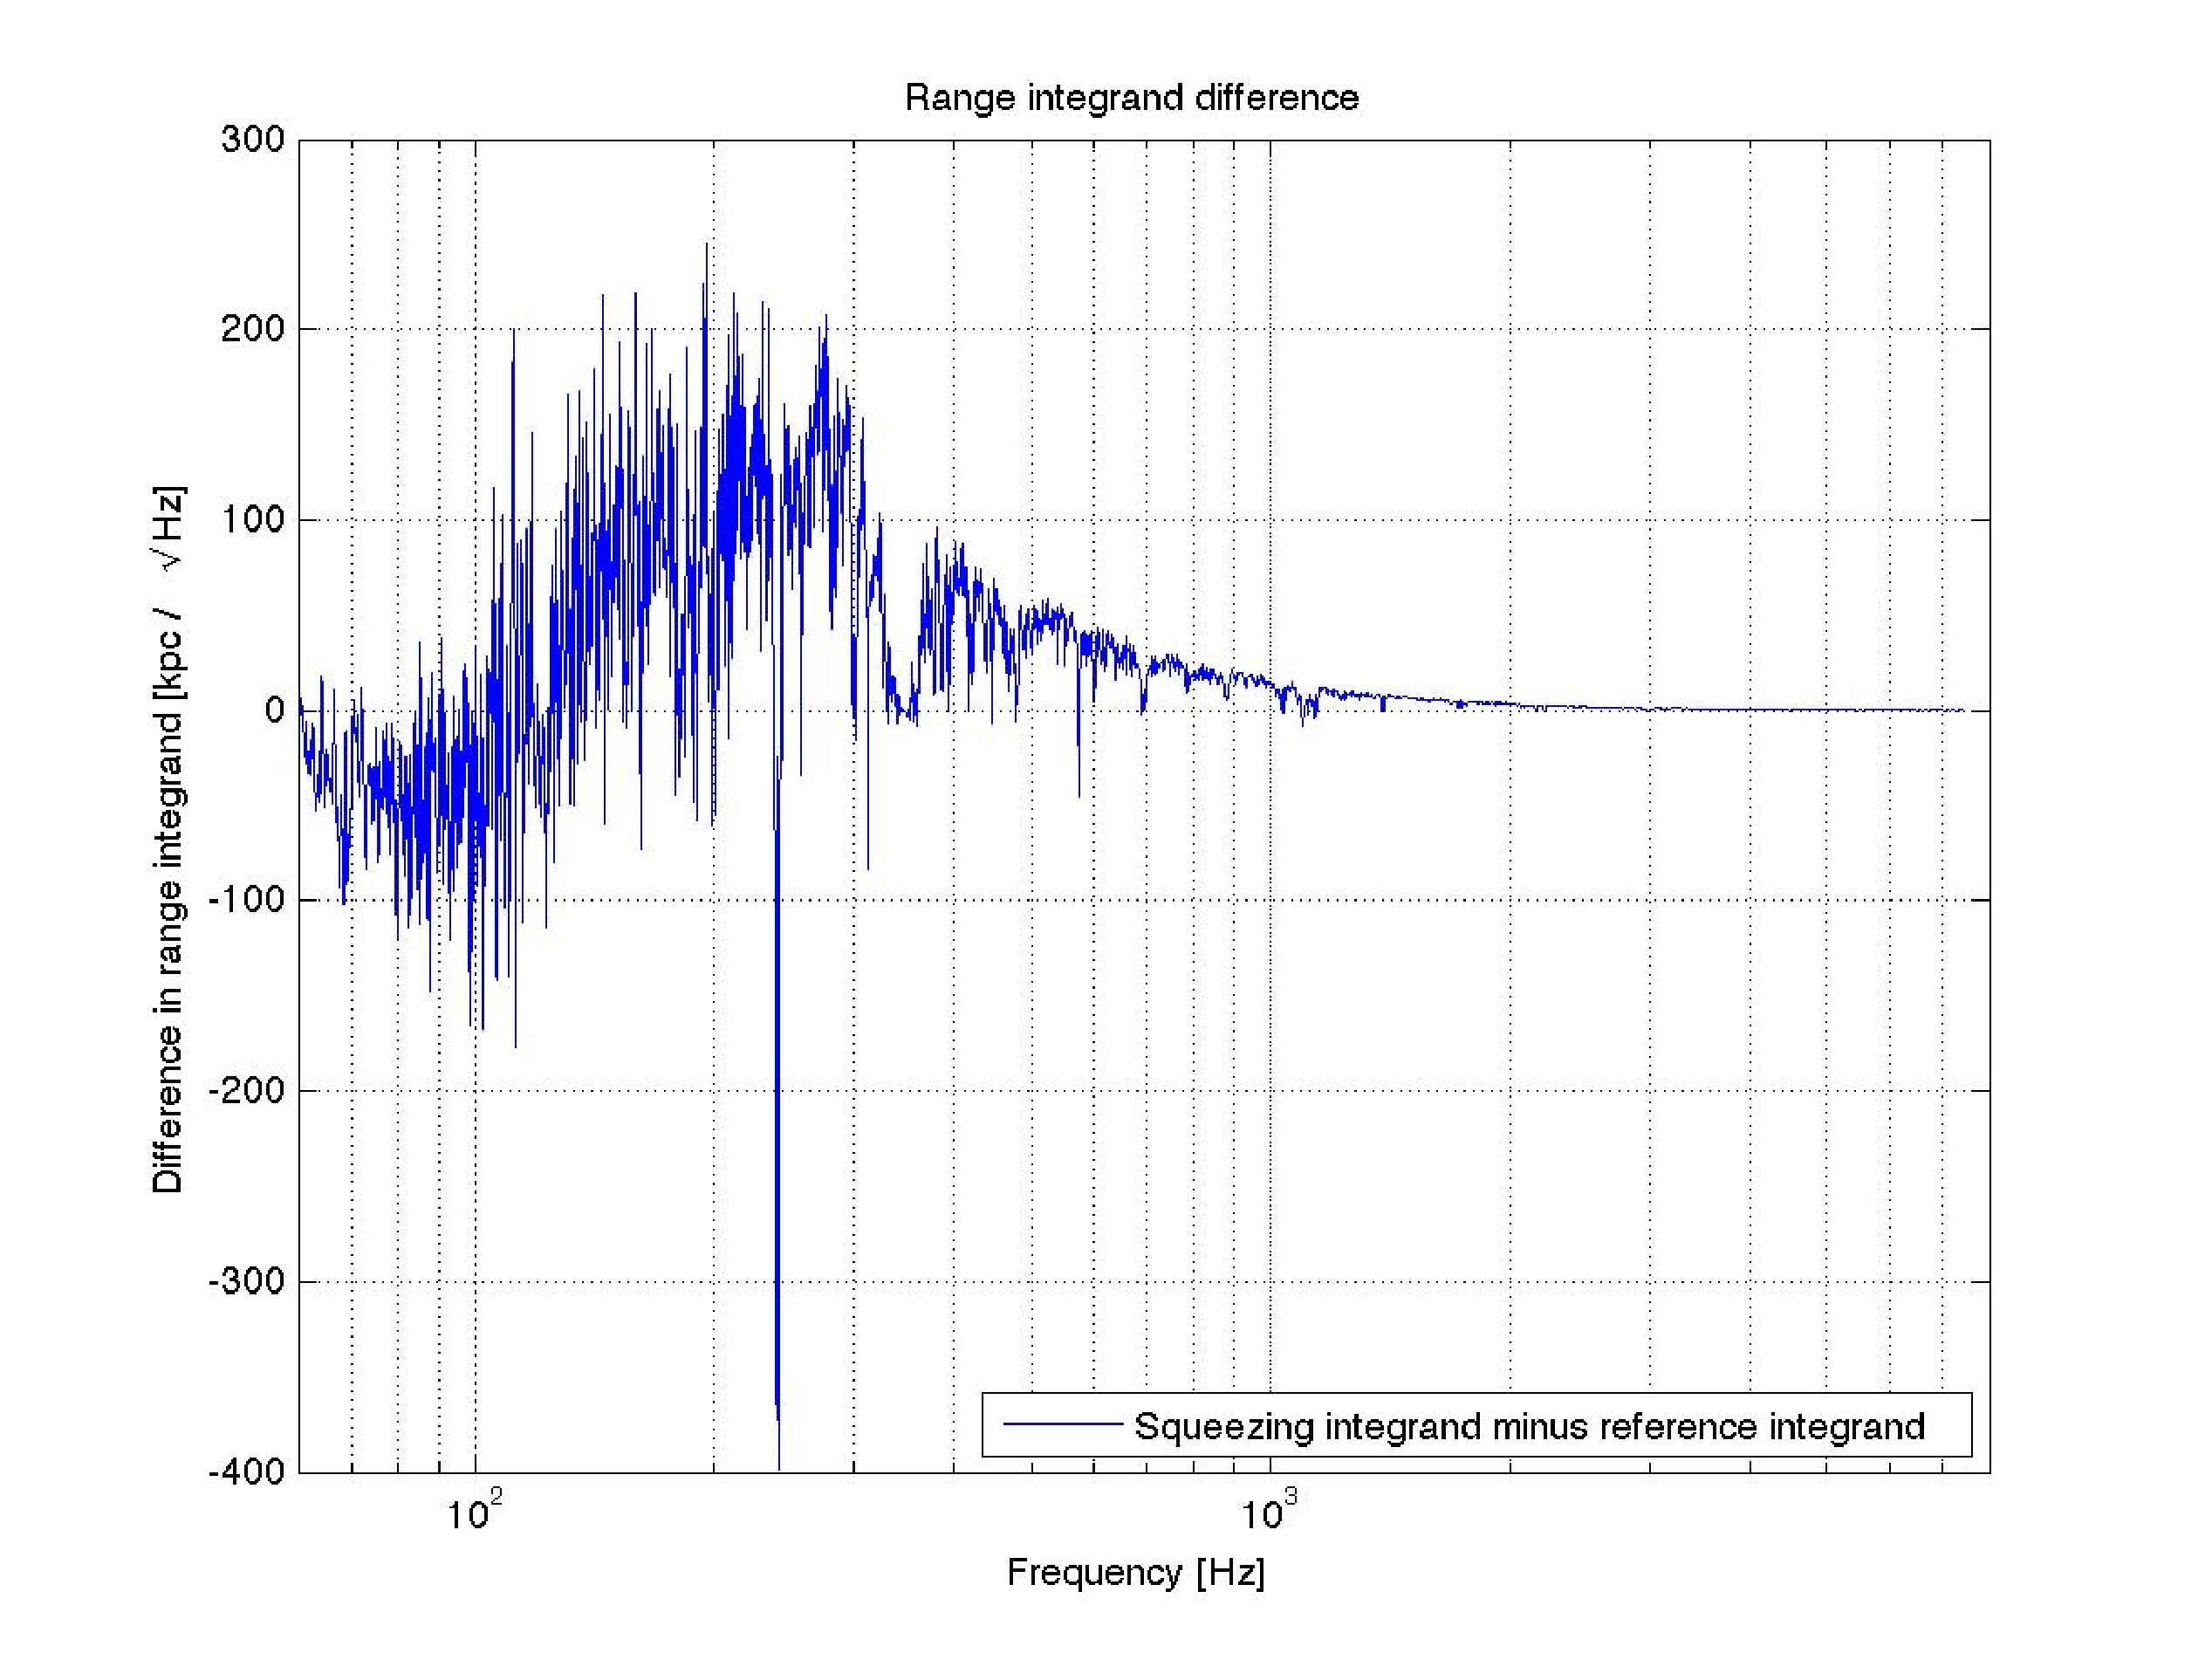
\includegraphics[height=0.5\paperheight, width=0.5\paperwidth,keepaspectratio]{range_integrand_difference.eps}
\caption{Net effect of squeezing on inspiral range integrand. Scientific benefit from squeezing is evident at the few hundred Hz `bucket' where initial LIGO is most sensitive, and although low frequency noise is slightly worse, this in an already noisy spectral band. Enhanced LIGO unambigiously benefitted from squeezing, proving the technique's efficacy.
}
\end{center}
\end{figure}




            \subsubsection{Figures of merit: inspiral range}
            \label{range_est}

                Range estimation after squeezing

		From the improved shot noise, we can see that squeezing at high frequencies bought enhanced LIGO a megaparsec of inspiral range. This number is impressive in several respects: our goal was to acheive a squeezing factor of perhaps as much as 3 dB, but to do it in the shot noise-limited region, at high frequencies, where the inspiral range equations (MATH: add the inspiral range equation if not already shown for feedforward!) count for much less. Morever, that range figure reflects the acheivement of squeezing down to 150 Hz, which is the lowest yet achieved for a gravitational wave interferometer, as can be seen in the Nature Photonics paper~\cite{BarsottiNatureSqueezing}


\section{Squeezing large interferometers}

        \subsection{Success and Advanced LIGO prospects}
        \label{squeezing_success}
            Results and hopes for aLIGO+ squeezing.

	    The squeezer group has a paper pending in review for Nature, written by Lisa Barsotti, in which we discuss our acheivement of perhaps 2 dB worth of squeezing (need to cite and check whether it is OK to use this number)~\cite{BarsottiNatureSqueezing}. It builds on the previous success of GEO600 in squeezing~\cite{GEO600NatureSqueezing}.

	    Discuss Sheila Dwyer's~\cite{DwyerPhaseNoise} and Sheon Chua's~\cite{ChuaBackscatteredLight} papers, since I am an author on both of them. We have a preliminary understanding now of at least two major problems: the quadrature phase noise fluctatuations and backscattered light. Backscattered light can be resolved in several ways. Phase noise must be progressively improved, as Sheila discusses, because we can hope to acheive the mature filter cavity design proposed below.

Discuss Lisa Barsotti's talk about the future prospect for LIGO using filter cavities, work that Tomoki Isogai is doing. With filter cavities, we can acheive frequency-dependent squeezing, having the best of both works by reducing quantum radiation pressure noise at low frequencies and shot noise at high, by using the filter cavity to produce a squeezed vacuum with a squeeze angle that varies as a function of frequency. Though as yet this filter cavity has yet to be constructed, it is in the works at MIT.

% Everything below is imported from my AEI talk




%\end{frame}

%\begin{frame}{Squeezing summary}
\subsection{Squeezing summary}

\begin{description}
\item [{Instrumental}] experience with technique important beyond Advanced
LIGO
\item [{Physical}] way to improve broad band of LIGO, benefit many searches
\item [{Illustrates}] need for best sensitivity at few hundred Hz
\item [{Question}] what can we improve \emph{post-facto?}
\end{description}
%\end{frame}


%        -------------------------------- 
%
%	The following is an example of using the commands \textit{ref}
%	and \textit{label}. With these commands theorems, chapters,
%	sections and figurres can be labeld with names in the tex file
%	and then refered to by these names in later tex files. In
%	chapter~\ref{intro} we saw section~\ref{sample_section} or
%	theorem~\ref{sample_theorem}.
%
%	Lastly, here is how to include a figure. First generate an
%	encapsulated postscript file in xfig, adobe illustrator or
%	some other program. The specific commands are found in
%	\textit{chap2.tex}.
%
%        \begin{figure}[htb]
%        \centerline{ \epsfig{figure=sample.eps, 
%        height =  1.5 in}}
%        \caption{Sample Figure}
%        \label{sample_figure}
%        \end{figure}


% Binary neutron star search
\chapter{Exhibit: World Science Festival}
\label{chap5}



        
        \section{Neutron stars in binary systems}
        \label{binary_NS}

Continuous waves from neutron stars in binary systems are distinctive.
As Section~\ref{continuous_waves} comments, binary systems constitute 211 of 379, or 55\%, of known pulsars with rotation frequency above 10 Hz and thus in the LIGO band (see the ATNF catalog, currently containing 2328 pulsars total~\cite{ManchesterATNF2005}).
CW search methods prove powerful, probing well below the LIGO amplitude spectral density (ASD) noise floor given year-length science runs, yet computationally-demanding.
A non-trivial possibility exists that there are CW from neutron stars (NS) in binary systems, buried in existing or forthcoming data, that could be seen with a fast, tractable search method.

TwoSpect~\cite{GoetzThesis,GoetzTwoSpectMethods2011,GoetzTwoSpectResults2014} is such a method. 
Developed as a search for neutron stars in binary systems with unknown sky location, orbital period, projected semi-major axis or frequency, it has been tested and run on S6 data.
In such a mode it accepts some degradation of sensitivity in order to scan the entire parameter space.
If some parameters are known, a deeper search becomes possible.
This chapter describes the development of this `directed' search and its application to a simulated data set (a `Mock Data Challenge' or MDC).
The next chapter summarizes the preliminary results when applied to data from the last science run, S6.

            %Astrophysical prospects for binary pulsar detection. 
            %Binary pulsars are perhaps our best hope for detecting continuous gravitational waves.

%\begin{frame}{Neutron stars in binary systems}
\subsection{Continuous gravitational waves from neutron stars}
%\begin{definition}
%Neutron star with a partner in a binary system, 
%e.g., a low-mass X-ray binary (LMXB)\end{definition}

%\begin{example}
%Scorpius X-1
%\end{example}

Choosing to pursue binary sources is itself a choice of search direction.
Neutron stars can be in isolated systems as well, for which many searches have been conducted (summarized in Section~\ref{continuous_waves}).
Yet isolated stars have several issues that make them challenging to detect.
Isolated stars have a finite lifetime (albeit many millions of years) over which they are hypothesized to emit detectable GWs.
During this detectable lifetime, they are losing energy to GWs -- this energy loss results in a continually slowing frequency, denoted by the spindown rate $\dot{f} = df /dt$.
GWs are not the only contributor to spindown: non-gravitational energy loss due to friction or magnetic interactions with an accretion disk will also sap the rotational energy of the star and thus its GW emission amplitude.
Non-GW losses broaden the uncertainty in spindown rate.
Spindown in turn makes GW searches more computationally challenging: templated-phase mismatch over a science run of many months is often significant enough to require additional templates to search over putative spindown values. 
Since many searches are already computationally limited, a GW source without these challenges would arouse interest.

Accreting binary systems generate such interest.
LMXBs, low-mass X-ray binaries, of which Scorpius X-1 (Sco X-1) is an exemplar, are at the focus.
As understood from the work of Papaloizou \& Pringle~\cite{PapaloizouPringle1978} and Wagoner~\cite{Wagoner1984}, LMXBs might exhibit several key properties:

\begin{itemize}
\item Longer GW lifetime than isolated sources, due to accretion recycling
\item Ellipticity \& hot spots, due to accretion
\item Hypothetical \textit{torque balance} frequencies
\end{itemize}

Not only are LMXBs an abundant fraction of the neutron star population, they also constitute a disproportionate quantity of fast period, \textit{millisecond} pulsars -- and interestingly may be capped at a speed limit (hypothesized by Chakrabarty~\cite{Chakrabarty2003}) below the relativistic breakup limit.
If so, LMXBs in particular would constitute an ideal search target.
Let us review the points of lifetime, ellipticity, and torque balance in further detail.

%Potential candidates for gravitational waves:
%\begin{itemize}
%\item Longer lifetime than isolated sources (recycling)
%\item Ellipticity \& hot spots due to accretion
%\item Torque balance hypothesis (Papaloizou \& Pringle 1978, Wagoner 1984):
%\item \emph{bright ms pulsars}
%\item Speed limit? (Chakrabarty 2003)
%\end{itemize}
%\end{frame}


            \subsection{Binary spin-up and detectable lifetime}
            \label{spin-up}
         
                %GW pulsar lifetime alone vs companion.
As stated, isolated, elliptical, rotating NS will lose energy to GWs.
This intrinsically makes their GW radiation short-lived.
Binary systems, in contrast, can be recycled by accretion.
Not necessarily a steady process, recycling of infalling matter from an orbital partner can raise the spin frequency of a neutron star by conservation of angular momentum.
Energy is released as heat and radiation on impact with the surface of the NS, in particular as X-rays in the case of an LMXB.
The work of Papaloizou, Pringle and Wagoner elucidates the implications for GW detection.
As infalling matter hits an NS, the matter stream can not only increase the spin frequency -- and thus GW radiation amplitude -- of the NS, but it can also increase NS ellipticity from matter accumulated at the hot spot.
Equation~\ref{cw_radiation_eps_eq} shows that this further increases radiated GW amplitude.
Insofar as the infall stream continues, the NS can be `spun-up' to rotation frequencies with non-negligible GW emission, potentially for a far longer detectable lifetime than an isolated star.

Spin-up might proceed, as Wagoner derives, only up to a specific frequency.
In this \textit{torque balance} hypothesis, the matter infall delivers a torque offset by angular momentum loss from GW emission; since GW emission rises with frequency, an NS that is spinning up due to accretion will eventually reach a limiting frequency beyond which GW emission prevents it from spinning faster.
This idea, developed by Bildsten~\cite{Bildsten1998}, connects accretion rate with GW emission.
Since accretion rate can be measured electromagnetically, in X-ray flux $F_\textup{X-ray}$, this lets us estimate what level of GW emission at frequency $f$ could be expected for a star rotating at frequency $\nu = f/2$ (Equation~\ref{torque_bal_eq} in general, Equation~\ref{ScoX1_torque_bal} for Scorpius X-1~\cite{GoetzThesis,Bildsten1998}): 

\begin{equation}
h_{0} \approx 5\times10^{-27}\left(\frac{300\textup{Hz}}{\nu}\right)^{1/2}\left(\frac{F_\textup{X-ray}}{10^{-8}\textup{erg cm}^{-2}\textup{s}^{-1}}\right)^{1/2},
\label{torque_bal_eq}
\end{equation}
\begin{equation}
h_{0} \approx 2.8\times10^{-26}\left(\frac{600\textup{Hz}}{f}\right)^{1/2}.
\label{ScoX1_torque_bal}
\end{equation}



\noindent Torque-balanced neutron stars would remain at their torque-balance frequency: accretion would counteract spindown.
This frequency stationarity is computationally useful.

            \subsection{Detection rate projections}
            \label{rate_projections}

                %aLIGO rate projections.
Equation~\ref{torque_bal_eq} is incentive to develop searches especially for LMXBs.
Although the predicted $h_0$ is still low, it is conceivable that high-luminosity sources such as Scorpius X-1 (see Section~\ref{scox1_parameters} for full parameters) or possible transients might just be within reach of advanced detectors such as aLIGO.
Unknown sources with potentially higher GW flux are a motivation for making this search capable of scanning the entire sky.
It is difficult to infer how many sources might exist, but over 50 accretion-powered X-ray pulsars were already known as of 2005~\cite{ManchesterATNF2005}.
Known, especially-promising sources such as Scorpius X-1 warrant scrutiny with a deeper, \textit{directed search} over their known parameter space.
Such searches are the purpose of TwoSpect.

        \section{TwoSpect searches}
        \label{all-sky}

TwoSpect offers a way to calculate a statistic and infer detection probability for a putative template waveform of a neutron star emitting continuous GWs in a binary system.
LIGO CW searches generally use matched filters, like inspiral searches. 
Although the CW filter is easier to calculate than inspiral filters for merging black holes, the net computational cost is much higher, since integration covers a much longer timespan, compensating for weaker signals. 
Matched filtering a binary pulsar search in the time-domain, with complete phase information, appears to be computationally intractable for terascale computer clusters in the early 2010s. 
By switching the problem to frequency domain power instead of amplitude, the search becomes feasible, albeit at a cost in sensitivity.

TwoSpect performs two transforms: it first parcels a science run (year-scale) into overlapping short Fourier Transforms (SFTs, hour-scale or less).
SFT frequency bins for a given data stretch are then adjusted to the frequency at the solar system barycenter, accounting for Doppler shifting that would be induced at the sky location, frequency, and time under investigation.
Each row of constant-barycentered frequency bins is then treated as a time series.
That time series is then Fourier transformed too -- the two in TwoSpect.
This transform yields a plane of pixels: the frequency-prime $f'$ vs frequency $f$ plane.
Goetz and Riles~\cite{GoetzTwoSpectMethods2011,GoetzThesis} developed this technique in the context of GWs.
The plane of pixels provides a tractable data set on which binary CW templates can be tested.

Detectable strain sensitivity $h$ scales poorly with time, $T^{-1/8}$, due to the double transform, instead of $T^{-1/2}$ for a coherent search or $T^{-1/4}$ for semi-coherent, but matched templating techniques are powerful enough that being able to use them is promising.
Goetz developed a noise-subtracted $R$-statistic to measure the cumulative power in each binary CW template.
This statistic follows a distribution as the sum of many $\chi$-squared distributions (see Taylor~\cite{taylor} as well as Casella and Berger~\cite{CasellaBerger2001} for statistical reference) and yields consistent $p$-values.
These $p$-values can be extrapolated from Davies' method, having been vetted by Monte Carlo~\cite{GoetzTwoSpectMethods2011}.
By providing these statistics, TwoSpect yields information on a large fraction of parameter space hereto unsearchable.
The code is open source and available online~\cite{LALAPPSrepo}.

%            TwoSpect methods as-is. These are described in detail in Evan Goetz's thesis~\cite{GoetzThesis}. %Note that the code is located on the web freely accessible in the LALApps repository~\cite{LALAPPSrepo}.

%For primers on error analysis and statistics, see Taylor~\cite{taylor} as well as Casella and Berger~\cite{Ca%sellaBerger2001}.

            \subsection{Two spectra: a double Fourier transform}
            \label{two_spectra}

       %         'Two spectra' -- FFT of periodograms reveals modulation of sine waves.

The double-Fourier transform is illustrated in Figures~\ref{tfplane-figure} and~\ref{ffplane-figure}.
Existing LIGO routines perform the steps needed to generate the first figure: SFTs are made in pre-processing and then barycentered.
TwoSpect then re-invokes the Fast Fourier Transform routines to transform the frequency vs time plane into a frequency vs frequency-prime plane.
Although GW phase information is lost (and, for now, templates ignore orbital phase), the resulting search domain is robust against spin wandering.

\begin{figure}
\begin{center}
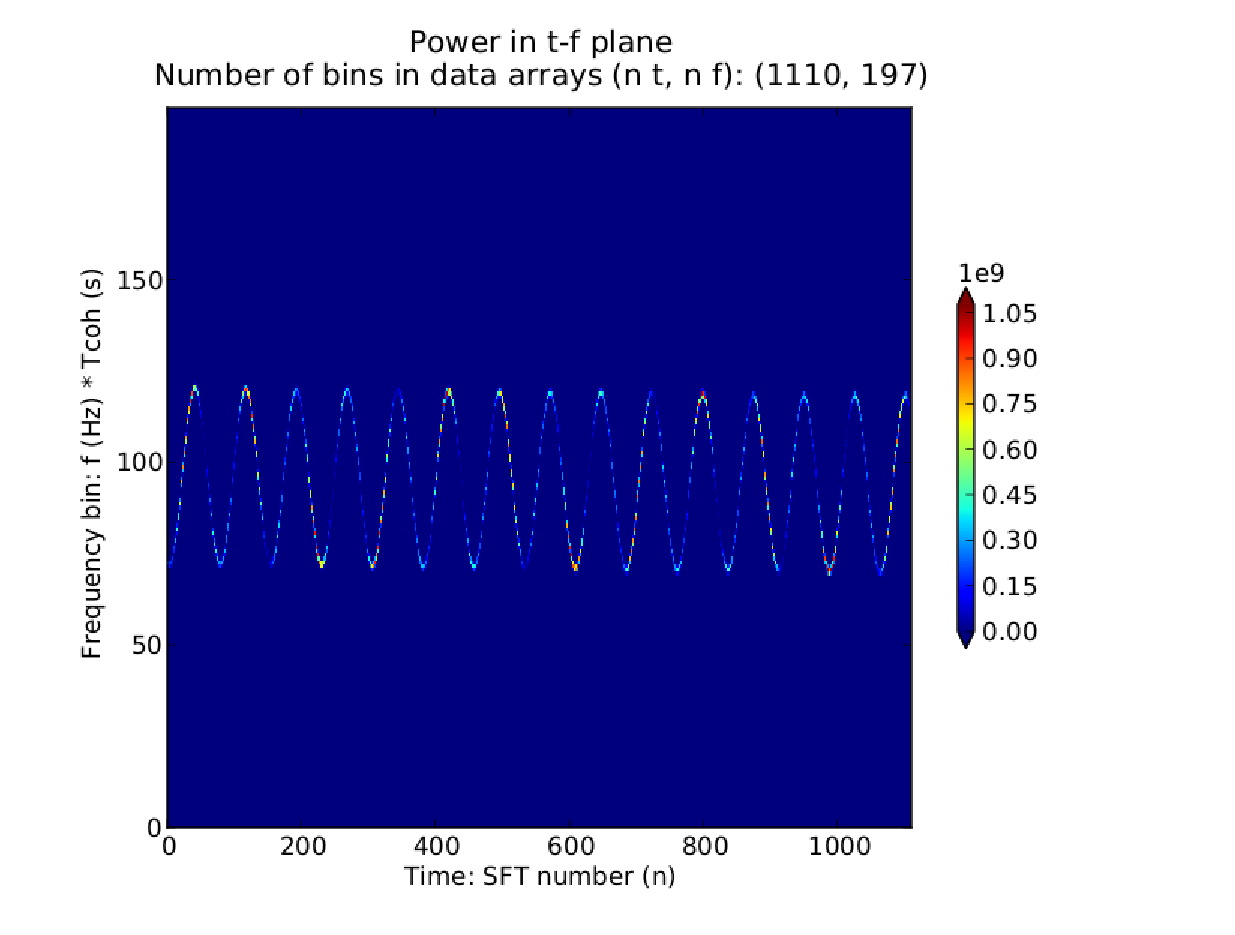
\includegraphics[trim=20 15 80 5, clip, width=0.7\paperwidth,height=0.35\paperheight]{tfplane-4e21-on-4e24.eps}
\caption{After Doppler-shifting the frequencies into the solar system barycenter, TwoSpect analyses begin on this first, time-frequency plane. A simulated signal at 100.015 Hz and $\textup{asini} = 1.44$ is injected with $h_0 = 4\times 10^{-21}$ into $10^6$ seconds of Gaussian noise at $Sh = 4 \times 10^{-24}$ (the projected minimum Advanced LIGO noise level); the signal period is 68023.8259 seconds, as with Scorpius X-1.}
\label{tfplane-figure}
\end{center}
\end{figure}

\begin{figure}
\begin{center}
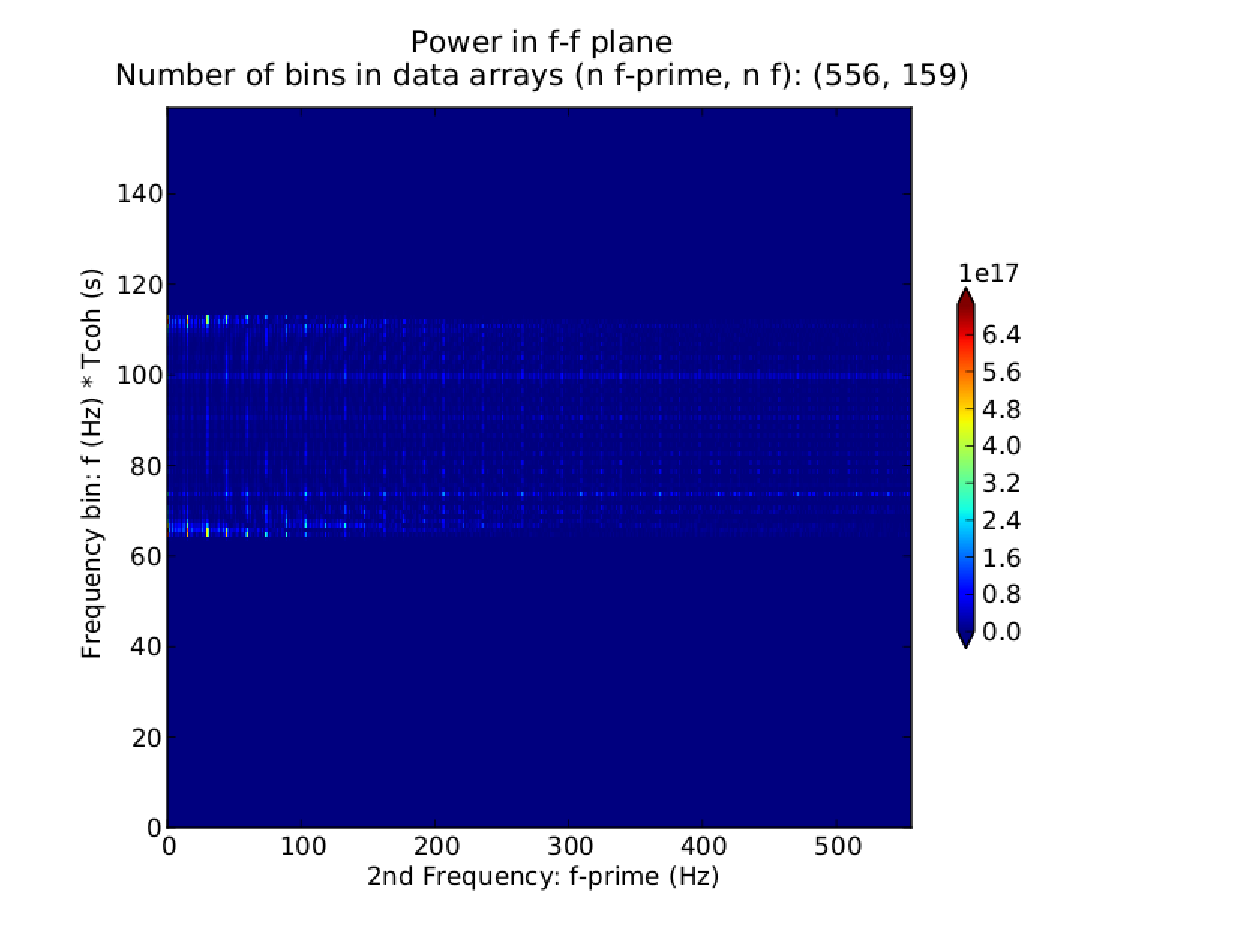
\includegraphics[trim=20 15 80 5, clip, width=0.7\paperwidth,height=0.35\paperheight]{ffplane-4e21-on-4e24.eps}
\caption{Fourier-transforming along the `rows' (constant frequency bin, variable time bin) generate a second plane, the frequency-frequency plane. The power of each bin in this transform is plotted as a pixel. By aggregating power, this second Fourier transform enhances signal so that matched templates can be applied for a search.}
\label{ffplane-figure}
\end{center}
\end{figure}

            \subsection{Inferring neutron stars with companions}
            \label{inference}
 
                %Infer whether modulation is due to a companion star.
With the search domain prepared, templates can be tested.
The modulation induced by LMXB partners on their NS companions is typically fractions of a Hertz.
Modulation depth is, more precisely~\cite{GoetzTwoSpectMethods2011},

\begin{equation}
\Delta f = \frac{2 \pi f (a \sin i)}{c P},
\label{TwoSpect_mod_depth}
\end{equation}

\noindent where $f$ is GW emission frequency, $a \sin i$ is projected semi-major axis, and $P$ is orbital period.
Equation~\ref{TwoSpect_mod_depth} specifies the amplitude of the sinusoid seen in Figure~\ref{tfplane-figure}, though it must be noted again that it is the power of the transform of that sinusoid in Figure~\ref{ffplane-figure} that is actually template-tested.


%\begin{frame}{TwoSpect algorithm for all-sky binary searches}
\subsection{TwoSpect algorithm detection statistic}

%TwoSpect (Goetz \& Riles 2011), supplied this  searches for patterns in
%doubly Fourier-transformed data from binary's orbital modulation
%\emph{doubly Fourier-transformed:} $k$ frequency bins, time series
%$n$
%Short Fourier Transform series, along $n$, is FFT'd 

Template-testing proceeds from a given test frequency $f$, modulation depth $\Delta f$ (via astrophysical $a \sin i$), and period $P$ using data prepared for some sky location. 
Having a time series $n$ SFTs long with $k$ frequency bins, a template weight can be computated for a number of pixels $M < n*k$.
Applying these weights yields the $R$-statistic:

\begin{equation}
R=\frac{\Sigma_{i=0}^{M-1}w_{i}[Z_{i}-\lambda_{i}]}{\Sigma_{i=0}^{M-1}[w_{i}]^{2}},
\label{TwoSpect_R_statistic}
\end{equation}

\noindent where
\begin{itemize}
\item $R$: template detection statistic
\item $w$: template weight
\item $i$: pixel index of $M$ pixels
\item $Z$: spectral power (after barycentric correction)
\item $\lambda$: expected noise power
\end{itemize}
%$\rightarrow$ E. Goetz wrote, conducting all-sky search
%\end{frame}
% Everything below is imported from my APS and AEI talks (harmonized)

\begin{figure}
\begin{center}
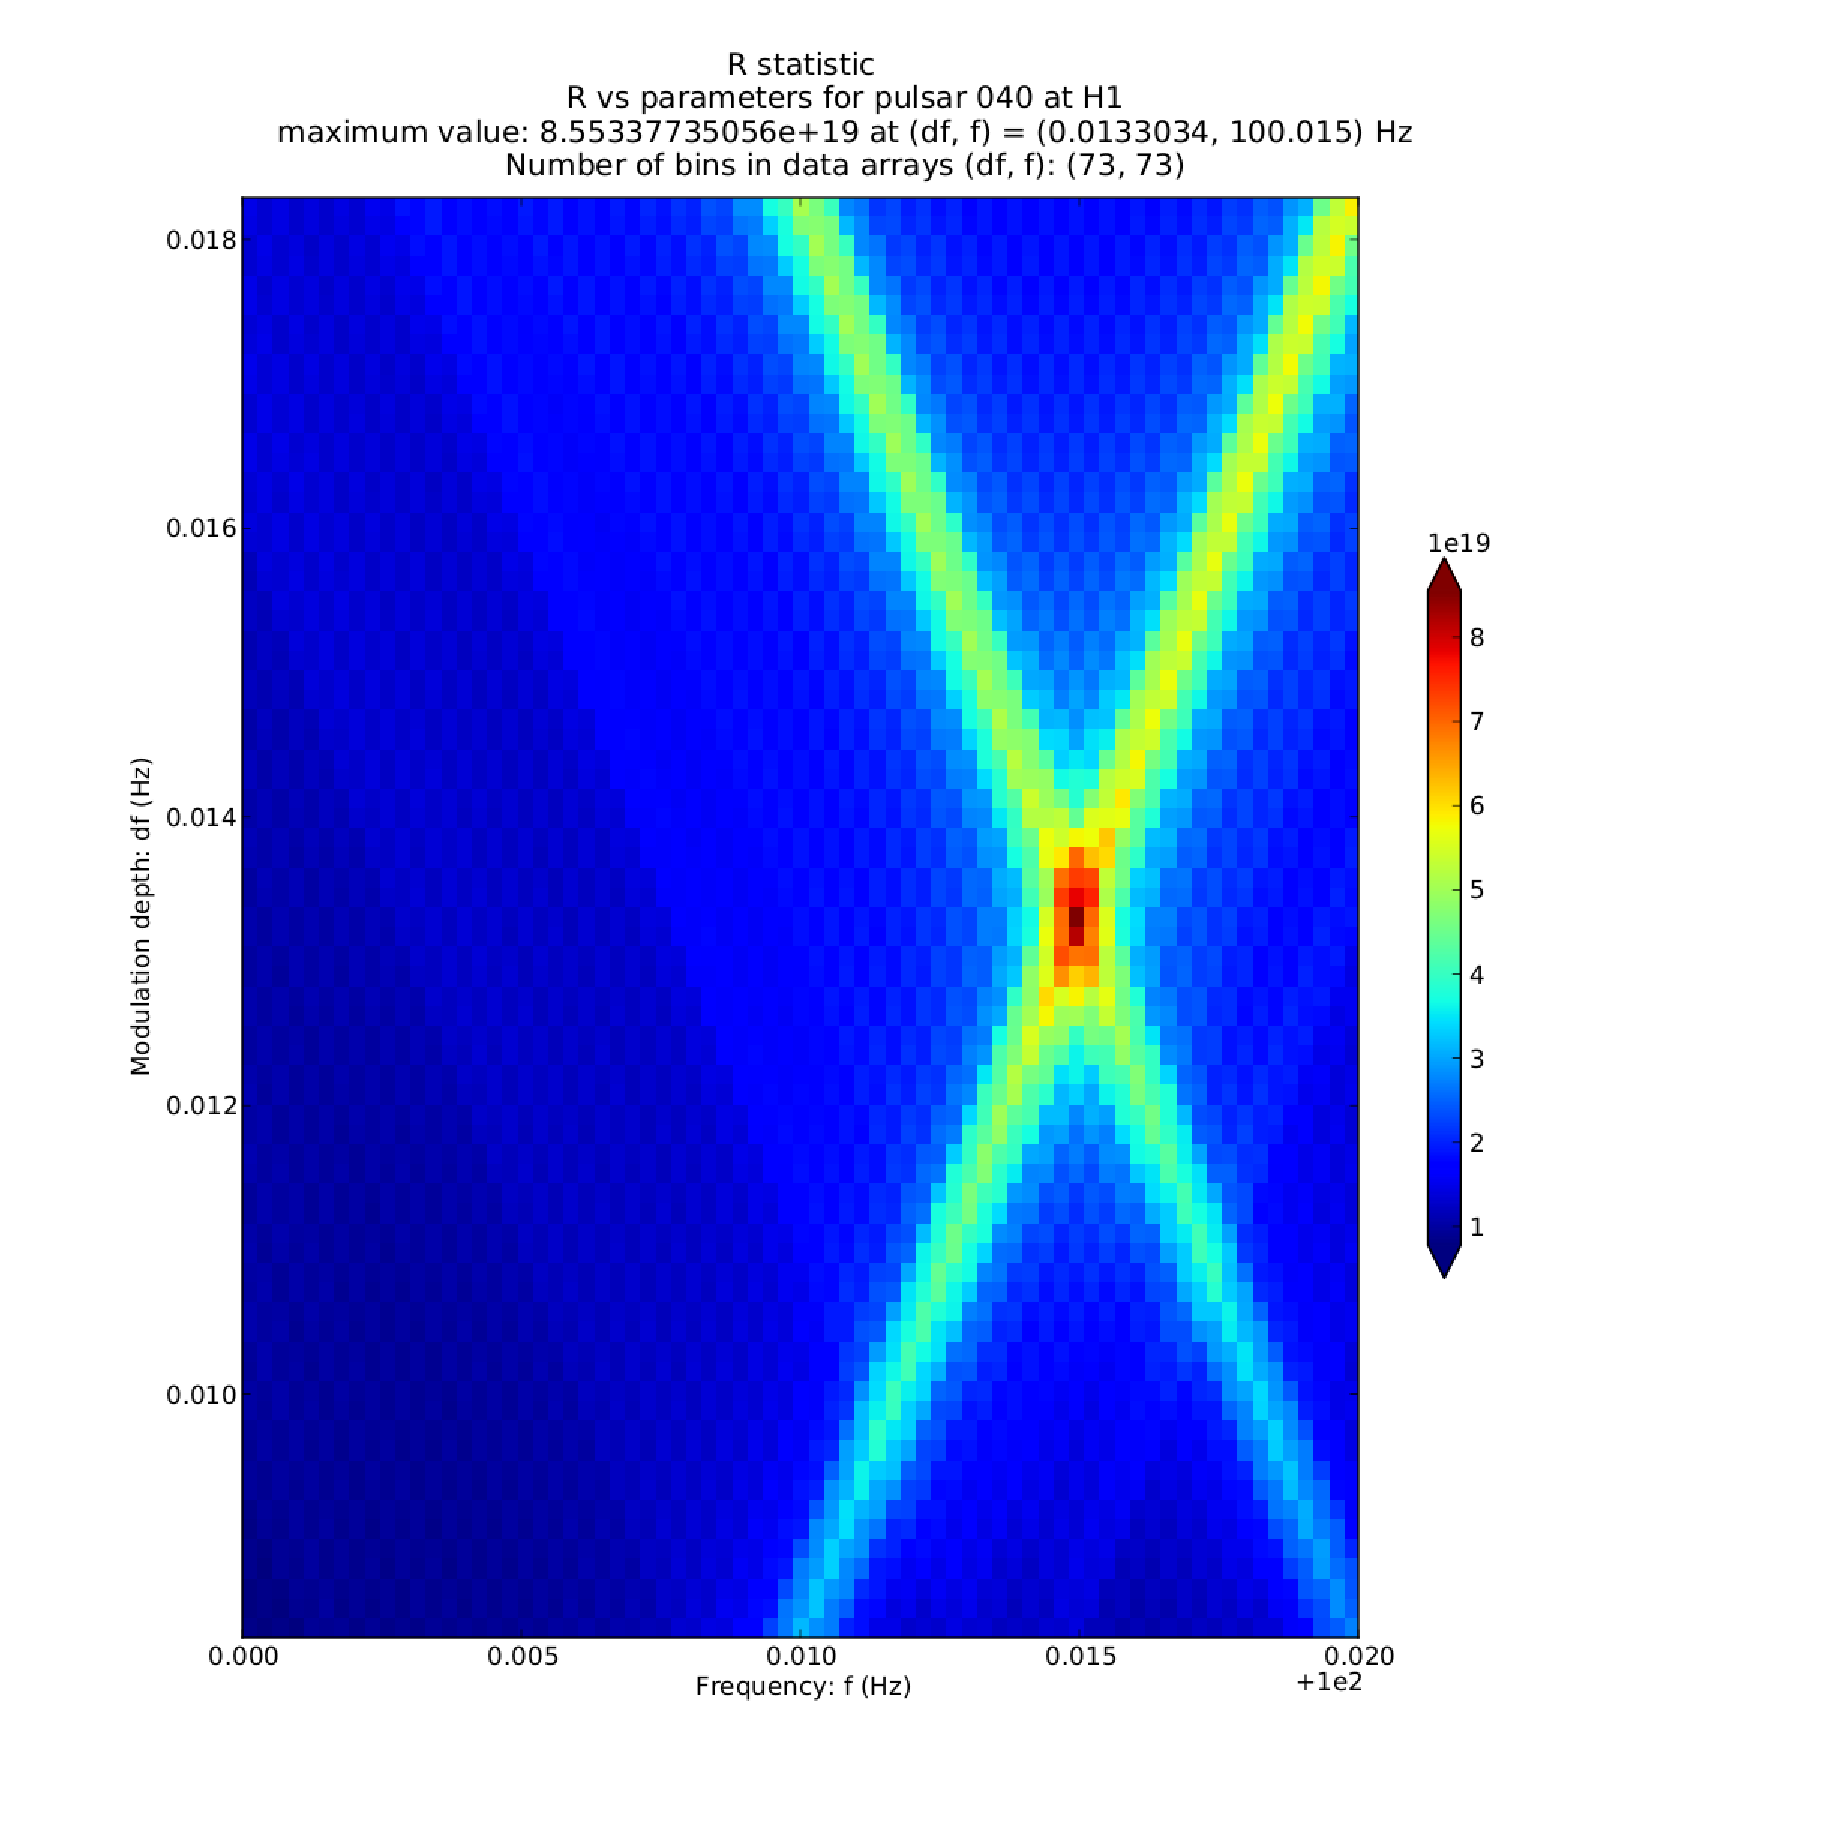
\includegraphics[trim=20 20 20 5, clip, width=0.8\paperwidth,height=0.62\paperheight]{R-4e21-on-4e24.eps}
\caption{Exact templates for putative singals weight the pixels in the frequency-frequency plane to generate $R$ statistic for a simulated pulsar (note: not the same as pulsar $40$ in the Scorpius X-1 mock data challenge) at 100.015 Hz and $\textup{asini} = 1.44$. The resulting $R$ values are heatmap-plotted on the modulation depth vs frequency plane.}
\label{inj_R_statistic}
\end{center}
\end{figure}

\begin{figure}
\begin{center}
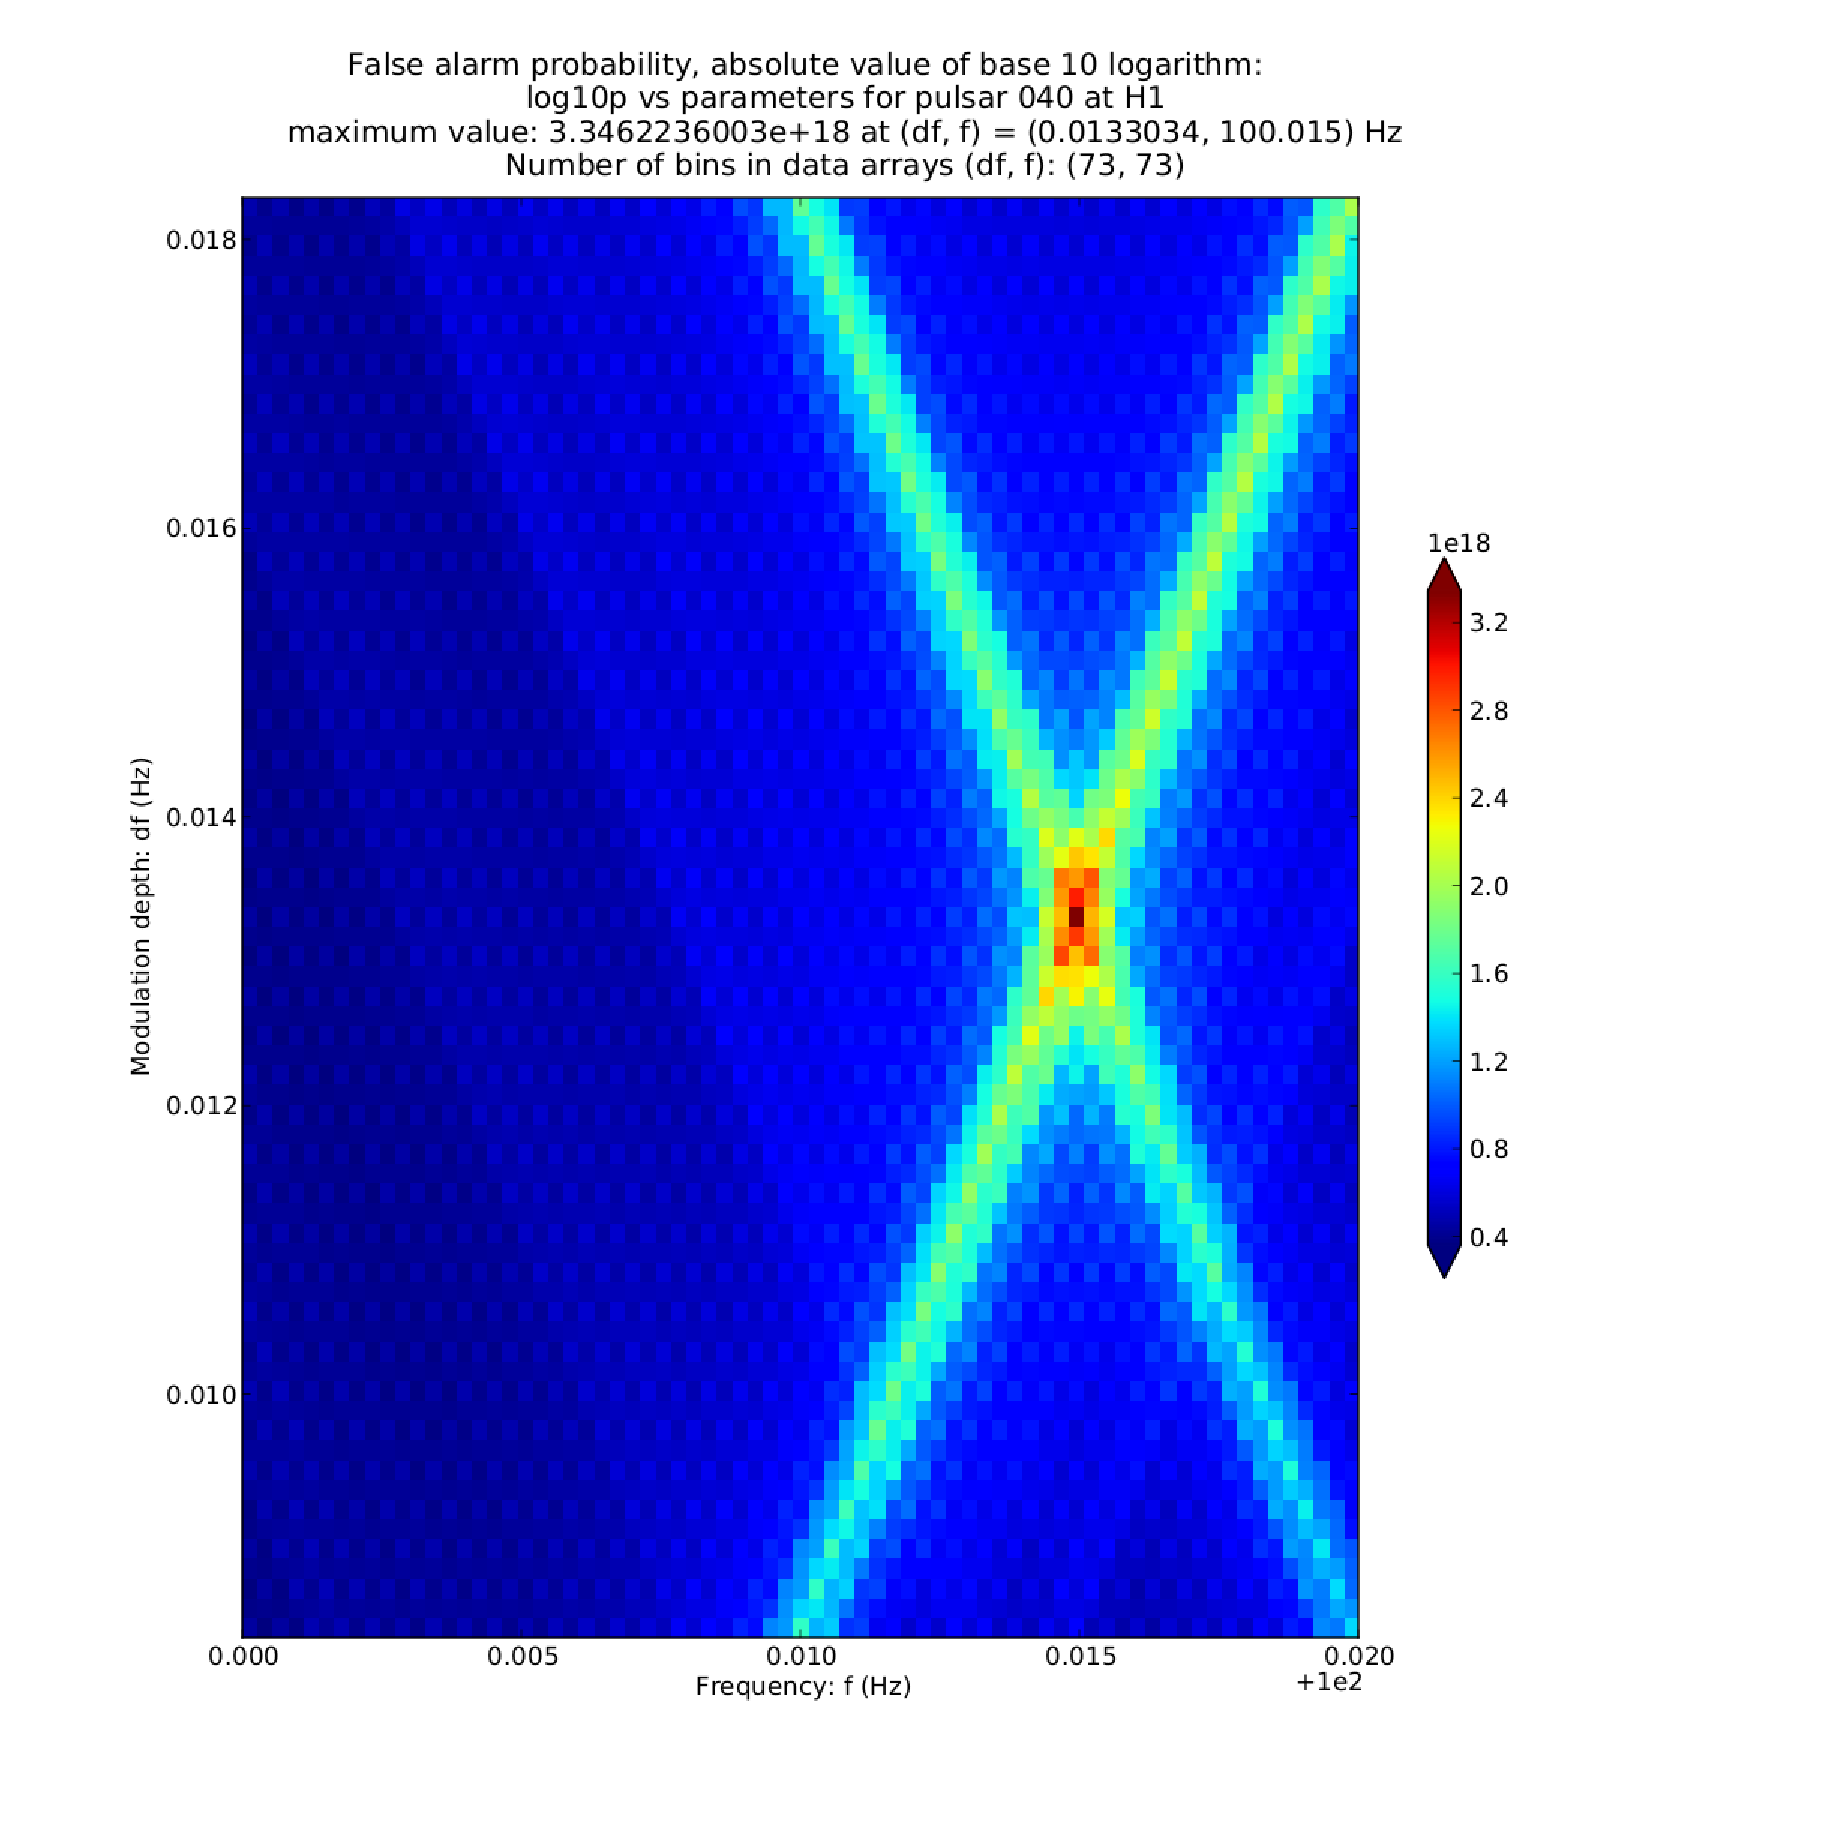
\includegraphics[trim=20 20 20 5, clip, width=0.8\paperwidth,height=0.62\paperheight]{Prob-4e21-on-4e24.eps}
\caption{The Davies algorithm translates $R$ statistic values for exact templates into (single-template) $p$-values, plotted on the modulation depth vs frequency plane.}
\label{inj_log10p}
\end{center}
\end{figure}

Testing various template models against simulated neutron stars in binary systems reveals the benefit of the $R$-statistic.
Figure~\ref{inj_R_statistic} shows that the statistic responds markedly when the input template values match the simulated `injection' sufficiently well.
The sharp response assures accurate parameter estimation.
Furthermore, Monte Carlo simulations by Goetz quantify the probability of high $R$ statistics arising from Gaussian noise.
Using generating functions and Davies' method, this probability has already been incorporated into a single-template $p$-value, seen in figure~\ref{inj_log10p}.
Further, multi-trial Monte Carlo studies done by the author have validated the probability of $R$- and $p$-values arising from Gaussian noise.


%\end{frame}

%\section{Directed searches for neutron stars in binary systems}

%\begin{frame}{Directed TwoSpect's greater sensitivity}
\section{Directed TwoSpect's greater sensitivity}

Searching over a wide range of right ascension and declination
%\footnote{Right ascension and declination date from at least the time of Ptolemy's \textit{Almagest} and are familiar in modern form in Copernicus's \textit{De revolutionibus orbium coelestium}~\cite{Hawking2002}. While ecliptic or more modern galactic coordinates can also be used, terrestrial Doppler motion is significant for CW searches and is most easily calculated in RA \& Dec.} 
can multiply computational times for gravitational wave searches by many orders of magnitude.
Each GW frequency needs to be corrected for Doppler shift and antenna pattern unique to each sky location.
%Historical interest: the system of right ascension and declination were fixed by the time of Corpernicus, \textit{De revolutionibus orbium coelestium}~\cite{Hawking2002}.
The number of distinct sky points needed is discretized by the allowed mismatch in sensitivity between points.
Typically, we search over the parameter space with a grid that allows a $0.2$ relative mismatch in $R$ statistic; the space is smooth enough that this grid can be smooth and rectangular.
Looking across all LIGO frequencies requires over $10^{18}$ templates, of order $\mathcal{O}(10^9)$ more templates~\cite{GoetzTwoSpectMethods2011} to do an all-sky analysis than a search at a single location and known period.
Thus the all-sky search is, in practice, only feasible when the $R$-statistic is the last in a stage of hierarchical statistics for candidate GW signals.
The initial stage of this hierarchy, an incoherent harmonic sum, is known~\cite{GoetzTwoSpectMethods2011} to reduce potential sensitivity.

A \textit{directed} search could be narrowly focused enough to calculate $R$-statistics for all interesting binary CW models for a point in the sky.
%There are several reasons to pursue more \textit{directed} searches in addition to the all-sky search.
With a known electromagnetic counterpart, such as an LMXB or X-ray transient (XTE), the parameter space can often be reduced to a particular sky location (known to a few milliradians or better) and period (known to fractions of a second).
Frequency may (as with XTE J1751-305~\cite{Markwardt2002}) or may not (as with Scorpius X-1~\cite{Galloway2014}) be known\footnote{At our 8.5 kiloparsec galactic radius~\cite{KerrLyndenBell1986} both these sources are located in the direction of the galactic center.}.
%\emph{All-sky search: }parameter space $\gg10^{18}$ templates
%\begin{itemize}
%\item Hierachical search; incoherent harmonic sum to consolidate\\
%parameter space, use templates to test interesting outliers
%\end{itemize}
%\emph{Directed search: }parameter space much smaller
%\begin{itemize}
%\item Fully template the parameter space for max sensitivity
%\end{itemize}
Let us consider a search for an object such  as Scorpius X-1 (P $\approx 68023.7 \textup{ s}$, $a \sin i \approx 1.44\pm0.18 \textup{ light-s}$). The number of templates needed to cover the parameter space at a mismatch of $0.2$ is known from studies that find a spacing of $1/(2 T_\textup{coh})$ in frequency and $1/(4 T_\textup{coh})$ in $a \sin i$ provided sufficient coverage, given coherence time $T_\textup{coh}$. 
Here, assume a search over $6\sigma_{a \sin i}$, that is, $\pm 3 \sigma$ around the known orbital parameter $a\sin i$. 
Then,

\begin{equation}
N_{\textup{{template}}}=\left[1+2f_{bw}T_{coh}\right] \left[ {\displaystyle \Sigma}_{j=1}^{j = \frac{f_{max} - f_{min}}{f_{bw}}} 1 + 2\pi\left(f_{min} + j f_{bw}\right) \frac{4 T_{coh}}{P} 6 \sigma_{a \sin i} \right],
\label{N_template_full}
\end{equation}

\noindent simplified,

\begin{equation}
N_{\textup{template}} = 2 \left(T_{coh} + \frac{1}{f_{bw}}\right)\left[ 1+\frac{4 \pi T_{coh}}{P} (6\sigma_{a \sin i})(f_{max} + f_{min} + f_{bw})\right] (f_{max} - f_{min})
\label{N_template_simple}
\end{equation}

\noindent for a single interferometer. 

$f_{bw}$ is the width of a single analysis band. 
At present, we use 0.1 Hz bands.
$N_{template}$ is $\mathcal{O}(10^{8})$ for 3 interferometers over a 500 Hz band given the Sco X-1 orbital parameters.
Such a search is tractable, since a single template test requires on the order of a second.
This search promises to be significantly more sensitive than the all-sky search.
We chose to test this new method first in a Mock Data Challenge (MDC).
This MDC lets us ascertain our sensitivity relative to other GW-search algorithms.
TwoSpect is 1 of up to 6 existing programs looking for 50 ``open'' and 50 ``closed/blind'' Sco X-1-like ``pulsars'' (LMXBs).
Full MDC results are the subject of a forthcoming paper.
The rest of this chapter expounds on the development and testing of methods in the course of this MDC.

%\end{frame}

%\begin{frame}{Sky maps using exact templates}
\subsection{Sky maps using exact templates}

\begin{figure}
\begin{center}
%\protect\caption{\protect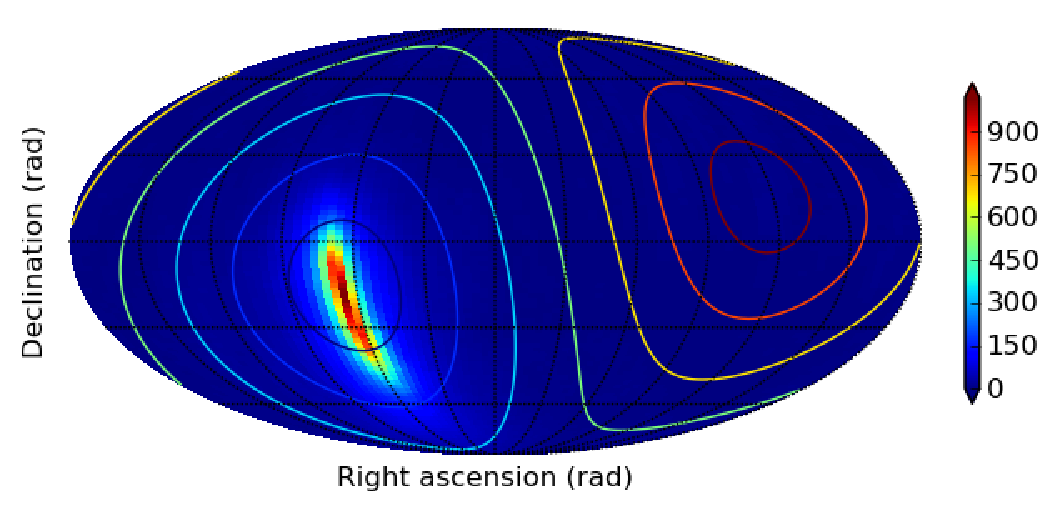
\includegraphics[width=0.4\paperwidth,height=0.2\paperheight]{maptrueH1}}
%\protect\caption{\protect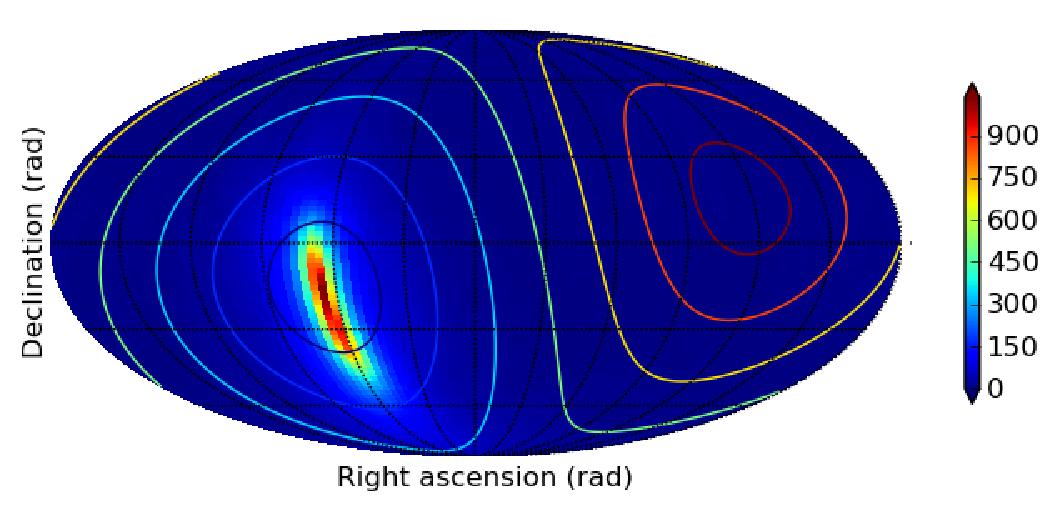
\includegraphics[width=0.4\paperwidth,height=0.2\paperheight]{maptrueL1}}
%\protect\caption{\protect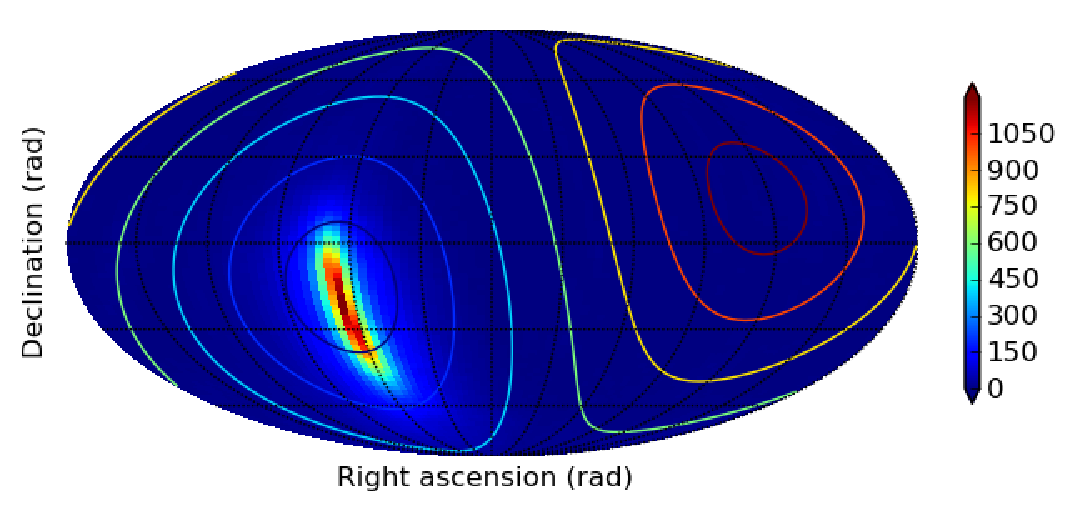
\includegraphics[width=0.4\paperwidth,height=0.2\paperheight]{maptrueV1}}
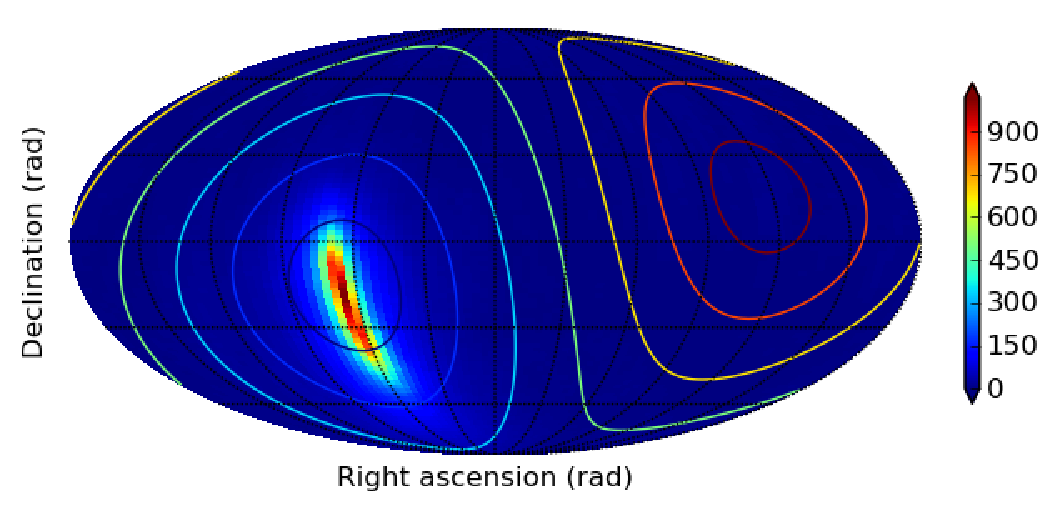
\includegraphics[width=0.6\paperwidth,height=0.2\paperheight]{maptrueH1.eps}
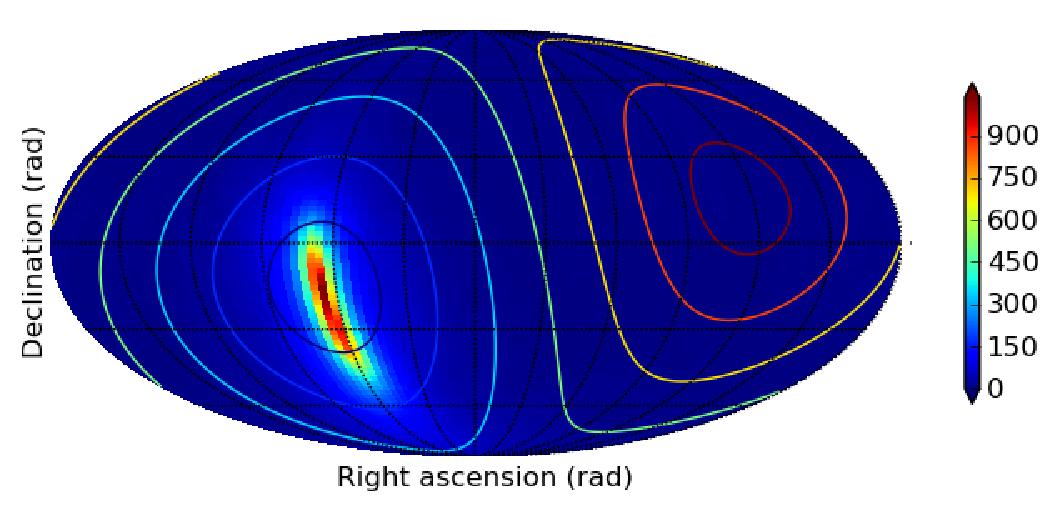
\includegraphics[width=0.6\paperwidth,height=0.2\paperheight]{maptrueL1.eps}
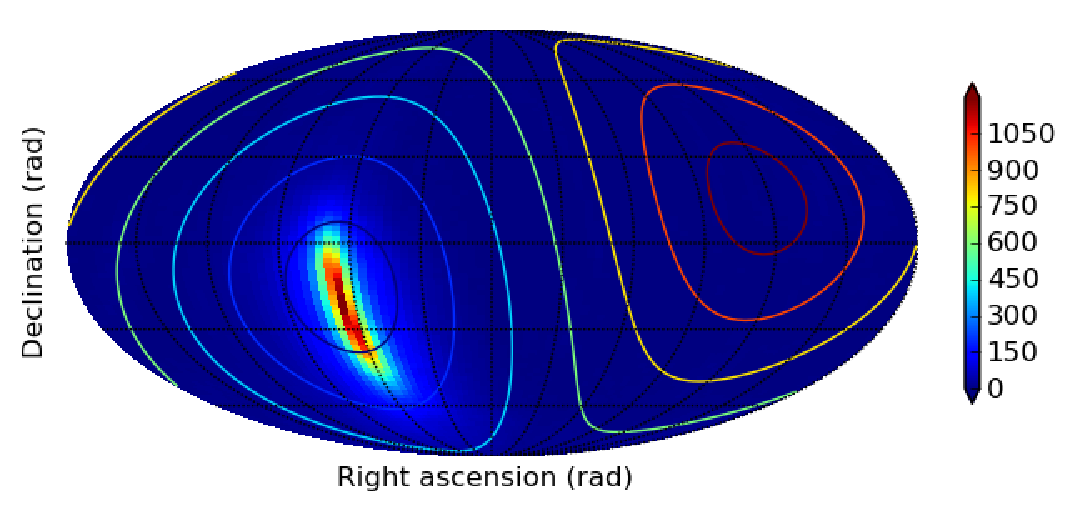
\includegraphics[width=0.6\paperwidth,height=0.2\paperheight]{maptrueV1.eps}
\caption{ All-sky maps, \{H1, L1, V1\} interferometer analysis from top to bottom, for template tests varying right ascension and declination. 
Scorpius X-1 mock data challenge pulsar 16 (101x101 templates), showing $\log_{10}p$-value on a Mollweide projection.
Contour lines at 1-radian great-circle distance intervals from the intended injection location of Sco X-1.
The results match the intended injection and confirm that the simulation is accurately representing the known sky location of Sco X-1.
}
\label{scox1-allsky-maps}
\end{center}
\end{figure}

At the beginning of the MDC, this author's work on TwoSpect played a key role in verifying that the simulation was correctly set up.
Although the author played no role in the data generation -- and was blinded to the parameters of the closed pulsars -- TwoSpect is sensitive both to relatively weak signals and to sky location.
Thus it was able to confirm that injected pulsars, as seen in Figure~\ref{scox1-allsky-maps}, were in fact in the expected location of a signal from Scorpius X-1.

%\end{frame}

\section{Scorpius X-1 mock data challenge}
%\begin{frame}{Fully-templated search for Scorpius X-1}
\subsection{Fully-templated search for Scorpius X-1}


\begin{figure}
\begin{center}
%\protect\caption{\protect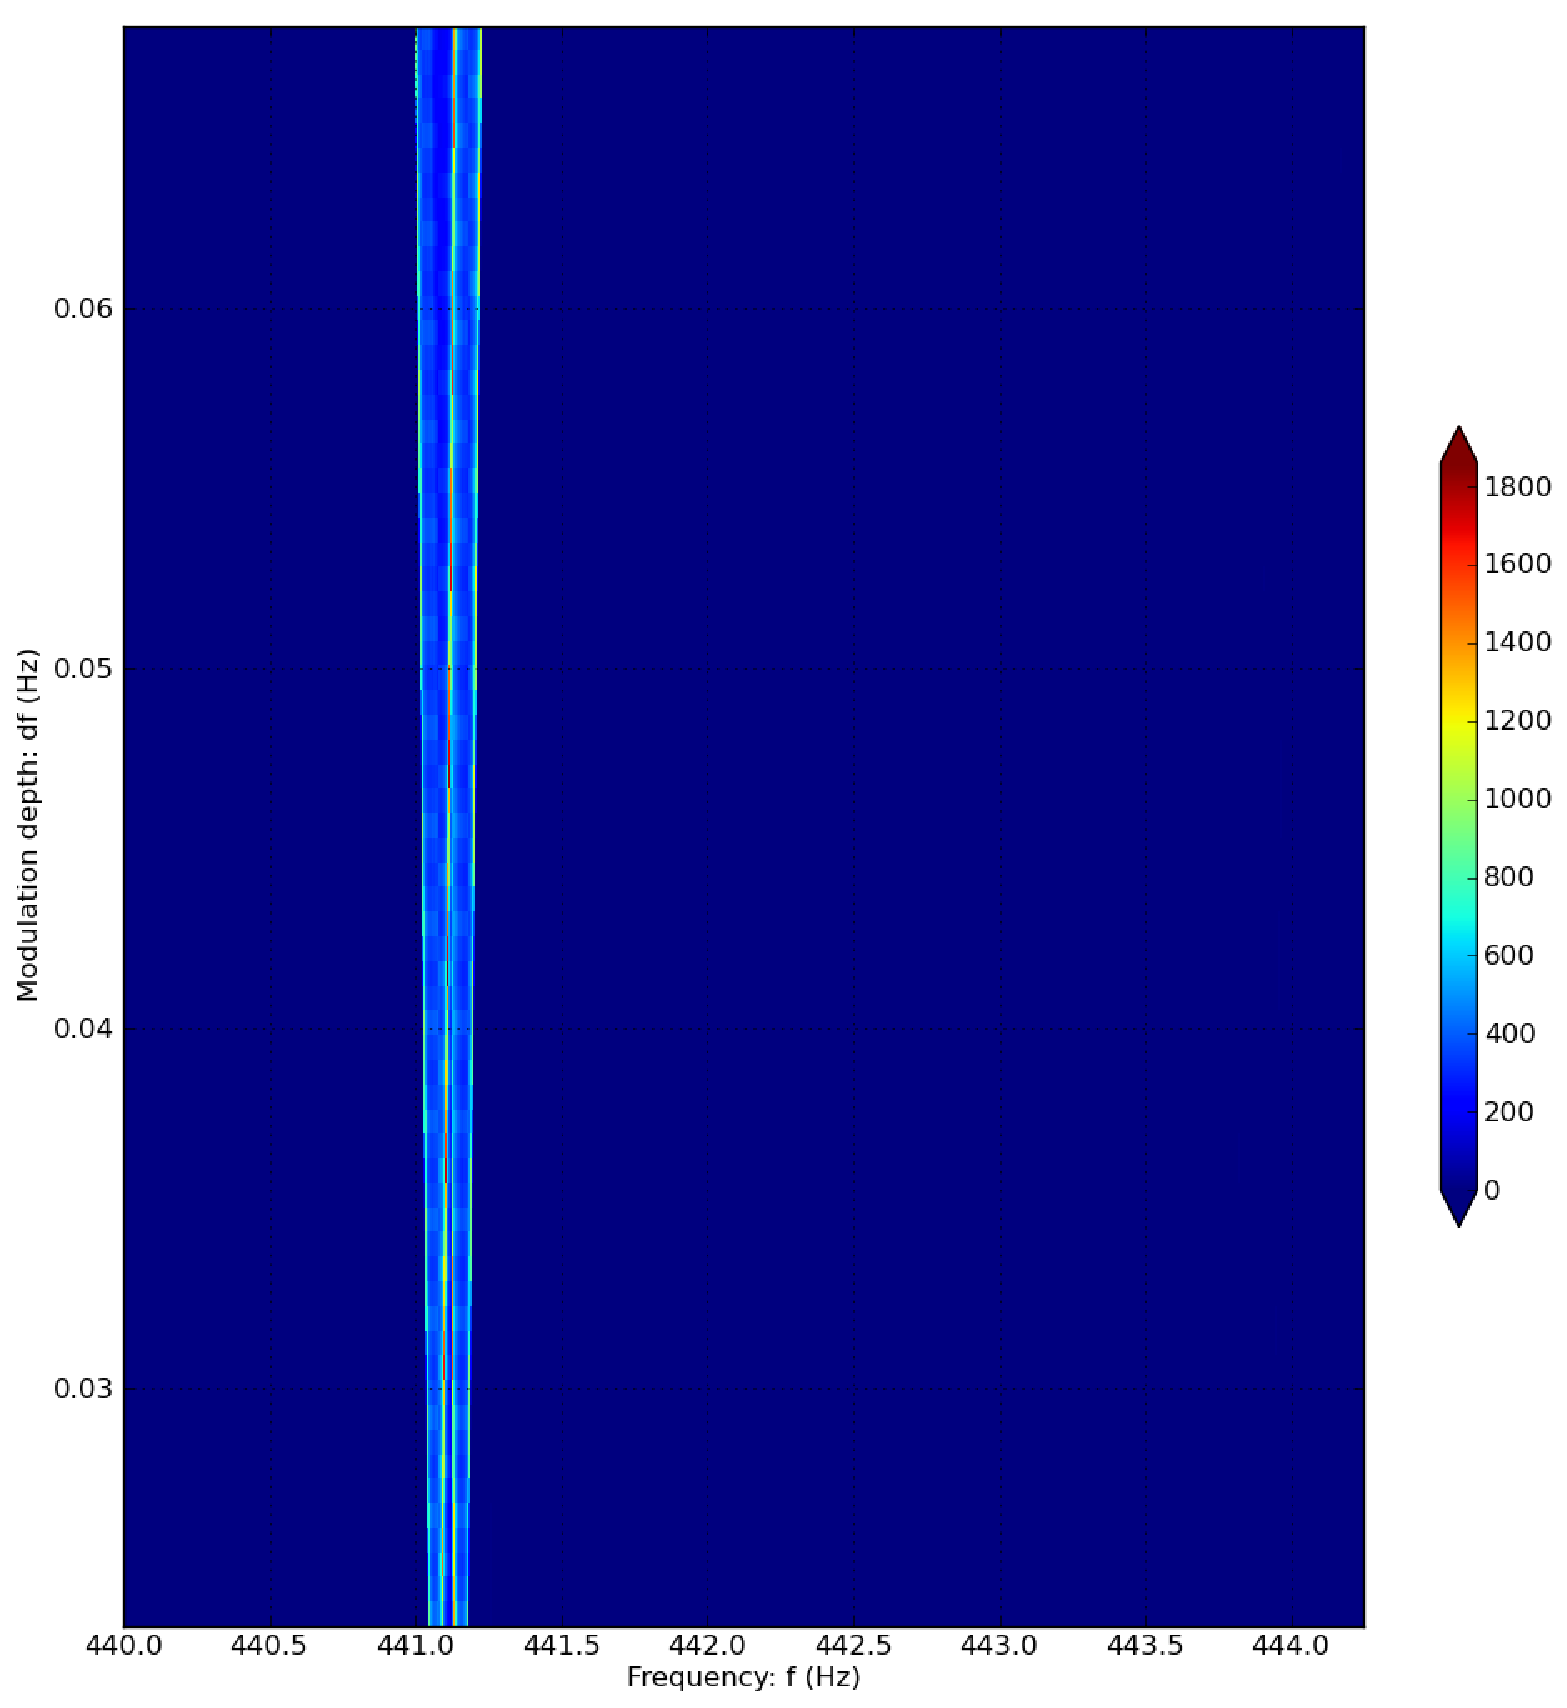
\includegraphics[width=0.8\paperwidth,height=0.62\paperheight]{bandH1-bold}}
\includegraphics[width=0.65\paperwidth,height=0.5\paperheight]{bandH1-bold.eps}
\caption{
Scorpius X-1 Mock Data Challenge (MDC) pulsar 40 \{H1\}: 5 Hz band. 
The $p$-value (single-template, applying Davies' Method to the $R$ statistic) in is show in this heatmap, peak in red. 
All templates are plotted on the (frequency, modulation depth) plane.
This is a relatively broadband view.
}
\label{scox1-wide-heatmap-040}
\end{center}
\end{figure}

Scorpius X-1 MDC data necessitated an efficient means of searching over a few hundred million putative templates using similar data streams from three interferometers (Hanford H1, Livingston L1, and Virgo V1).
Ideally, all one hundred 5-Hz search bands would be illuminated in the manner of Figure~\ref{scox1-wide-heatmap-040}.
Achieving this goal required some development by the author.

%\end{frame}

%\begin{frame}{Narrow-band heat maps in parameter space}
\subsection{Narrow-band heat maps in parameter space}


\begin{figure}
\begin{center}
%\protect\caption{\protect\includegraphics[width=0.4\paperwidth,height=0.2\paperheight]{heatmapH1}}
%\protect\caption{\protect\includegraphics[width=0.4\paperwidth,height=0.2\paperheight]{heatmapL1}}
%\protect\caption{\protect\includegraphics[width=0.4\paperwidth,height=0.2\paperheight]{heatmapV1}}
\includegraphics[width=0.6\paperwidth,height=0.2\paperheight]{heatmapH1.eps}
\includegraphics[width=0.6\paperwidth,height=0.2\paperheight]{heatmapL1.eps}
\includegraphics[width=0.6\paperwidth,height=0.2\paperheight]{heatmapV1.eps}
\caption{Heatmaps \{H1, L1, V1\} of 11x11 templates centered around
Scorpius X-1 MDC pulsar 8. 
This is a relatively narrowband view.
}
\label{scox1-narrow-heatmap-008}
\end{center}
\end{figure}

Initially, TwoSpect was configured for all-sky searches with the capability to bypass the incoherent harmonic sum and test a single point in parameter space.
It was possible to test multiple templates only by rerunning the entire TwoSpect pipeline.
Initial input/output loaded and Doppler-shifting made this highly wasteful, although it was possible to obtain results in narrow regions around which the unblinded, open MDC pulsars were specified.
Figure~\ref{scox1-narrow-heatmap-008} illustrates one such result.

%\end{frame}

%\begin{frame}{Wide-band heat maps in parameter space}
\subsection{Wide-band heat maps in parameter space}

\begin{figure}
\begin{center}
%\protect\caption{\protect\includegraphics[width=0.8\paperwidth,height=0.62\paperheight]{bandH1}}
\includegraphics[width=0.65\paperwidth,height=0.5\paperheight]{bandH1.eps}
\caption{Scorpius X-1 MDC pulsar 8 \{H1\}: 5 Hz band. This heatmap shows $3.6\times10^{5}$ templates, 10 to 22 mHz modulation depth, 120-125 Hz frequency. The peak signal at about (df = 0.019, f = 121.9) Hz.
}
\label{scox1-wide-heatmap-008}
\end{center}
\end{figure}

The author's first contribution to the pipeline was streamlining searching over arbitrary-width frequency bands.
Input/output is now done only once for a given search band, as is Doppler-shifting, expediting the testing of many templates for the $R$-statistic by several orders of magnitude.
While testing so many templates is arguably unnecessary -- the results are highly correlated -- it is computationally straightforward and yields the best gain in sensitivity over previous searches.
Figure~\ref{scox1-wide-heatmap-008} shows that these results match up with prior work, from Figure~\ref{scox1-narrow-heatmap-008}.

Whereas much existing TwoSpect post-processing to data had been focused on follow-up of all-sky results, parts of the directed search post-processing have needed to be re-invented.
The MDC validated these methods.

%\end{frame}

%\begin{frame}{Revisiting \& refining detection criteria}
\subsection{Revisiting \& refining detection criteria}


\begin{figure}
\begin{center}
%\protect\caption{\protect\includegraphics[width=0.45\paperwidth,height=0.45\paperheight]{StatHistRH1}\protect\includegraphics[width=0.45\paperwidth,height=0.45\paperheight]{StatHistProbH1}}
\includegraphics[width=0.6\paperwidth,height=0.35\paperheight]{StatHistRH1.eps}
\includegraphics[width=0.6\paperwidth,height=0.35\paperheight]{StatHistProbH1.eps}
\caption{Scorpius X-1 MDC statistics. These histograms of the $R$ statistic and $p$-value distribution helped in understanding noise, temporal gap \& spectral leakage, as well as establishing a threshold $p$-value $\sim$ false alarm probability of 1\%.
These $p$-values are for single templates, appropriate to the all-sky search but not to a dense templated search with a large trials factor.
Here, histograms show statistics in the absence of a signal. 
The left-skew of the $p$-values is associated with gaps in the data (as is right-skew, with different gaps).
Diurnal bias in barycentering is assumed, but the correlation is not fully understood.
}
\end{center}
\end{figure}



Running TwoSpect as a directed-search algorithm involves calculating
the $R$-detection statistic across the probable parameter space. 
A search is conducted with templates for each grid point in the Scorpius 
X-1 parameter space; period is known sufficiently well to restrict the search
to the two dimensions of signal frequency and frequency modulation. The
grid spacing, inversely proportional to spectrum coherence time, was
chosen to allow a mismatch no more than $0.2$ in the detection statistic.
Because of known period and sky location, the incoherent harmonic sum stage
of TwoSpect, used for the all-sky search, was bypassed entirely. 

\section{Mock Data Challenge procedure}

Each interferometer in the data challenge was analyzed individually for 
the detection statistic and corresponding single-template $p$-value. A set
of highest $p$-value outliers in 5 Hz bands was produced for each 
interferometer, subject to a $p$-value threshold inferred from Gaussian noise.
These sets were compared in pairwise coincidence (H1-L1, H1-V1, or L1-V1),
where coincidence required proximity within a few grid points in the 
parameter space. Any surviving outliers were classified as detections. 

The highest $p$-value outlier in a single interferometer in that band 
yielded the estimated parameters. Uncertainties in these parameters were also
determined from unblinded injections, using method of moments for signal
frequency and modulation depth and confidence intervals for signal
amplitude. Upper limits were declared from the best estimate of the 95\%
 confidence level of non-detected, unblinded, injected signals. The
largest uncertainty in upper limits and signal amplitude estimation derives
from the ambiguity between true $h_0$ signal and $\cos \iota$ inclination.
This ambiguity cannot be resolved with the present algorithm and depends
partially on the assumed prior distribution of signal ampltitudes; the
uncertainty was estimated by simulation.

Put another way, TwoSpect
in its directed search mode, tests templates with a model of
$f$, $a \sin i$, and $P$, as well as sky location. The latter two are
fixed for Scorpius X-1, as they are well-known. 
The $R$-statistic is not sensitive to time of ascension.
If a coincident detection is made between any interferometer pair in a 5 Hz band,
model parameters are read off from the extremal $p$-value template at
any one interferometer; $h_0$ is proportional to the quarter-root of
the test statistic. Uncertainty in $f$ and $a \sin i$ is determined
from the standard deviation of known injections; it is on the scale
of the template grid except for marginally detected pulsars. The $h_0$ 
uncertainty is largely due to the uncertainty in $\cos \iota$. 

%TwoSpect claimed to detect 34 of 50 blinded signals, as well as 31 of 50 unblinded signals, and it stated a flat
%$4.23 \times 10^{-25}$ upper limit for the 16 non-detected signals. 

\subsection{Detection Claims}

After studying the Gaussian noise in the Scorpius X-1 MDC open data set, we were able to set thresholds for detection claims.

TwoSpect's $R$-statistic and $p$-value space on the {frequency} vs {modulation depth} plane showed significant structures, particular around loud injections. These structures corresponded to the distribution of power into pixels by way of modulation depth, Earth's Doppler motion, and possibly spectral leakage. These regions of the open data set parameter space were excised before proceeding with the Gaussian noise study.

TwoSpect also found later-explained differences in the noise between the 360-s SFTs, used for pulsar bands above 360 Hz, and the 840-s SFTs, used for those bands below. 
The shorter SFTs were ostensibly noisier, requiring a more extreme $log_{10}p$ of $-12.0$, rather than $-7.75$ as in the longer SFTs, to cut single-IFO outliers and prevent any false alarms from surviving the coincident test between IFOs.
On revisiting the issue after the MDC, it was found that a misconfiguration bug explains the discrepancy (along with the larger number of templates and imprecise order statistics).
With the bug-contaminated Gaussian noise excluded, removing 3 million of 21 million Gaussian noise templates, the required $\log_{10}p$ for 360-s SFTs would only be $-8.80$.
This conclusion is consistent with our expectation that the $p$-value calculation should be independent of coherence time.

After studying the effect of pairwise coincidence requirements on surviving Gaussian noise outliers, we were satisfied that we would achieve a false alarm rate of 0.01 or better by setting the following detection criteria. 
Note that the $\log_{10} p$ values refer to single-template $p$-values; nearby templates are correlated in the presence of signal.

\subsection{Detection criteria}

\begin{itemize}
\item single-IFO candidates are the up-to-200 most extreme $p$-value outliers in a 5-Hz band that had a $\log_{10}p \leq$ threshold, where threshold = $-7.75$ if $f <$ 360.0 Hz (those that used 840-s SFTs) or $-12.0$ if $f \geq$ 360.0 Hz (those that used 360-s SFTs).
\item each candidate must survive at least one double-IFO coincidence test, involving a pairwise comparison of single-IFO candidates to see whether they are within 1/$T_{\textup{SFT}}$ in both frequency ($f$) and modulation depth ($df$).
\end{itemize}

$\rightarrow$ if there is any candidate surviving these criteria in a 5 Hz band, we mark detected, else not detected.

\subsection{Parameter Estimation}

MDC data allowed checking TwoSpect's parameter estimation on the 31 pulsars detected in the open data set.

Note that the $h_0$ reported in this section had not yet been recalibrated for either the $\cos \iota$ ambiguity due to assumed circular polarization (see subsequent section, factor of 1.74) or a systematic rescaling endemic to TwoSpect (factor of 1.11). 
Instead, the first step was to rescale the known $h_0$-injected from the MDC open data table into an $h_0$-effective. 
This $h_0$-effective equaled,

\begin{equation} h_{0-\textup{effective}} = \frac{1}{\sqrt{2}}\sqrt{ \left(\frac{1+\cos^2 \iota}{2}\right)^2 + \left(\cos \iota\right)^2 } \times h_{0\textup{-injected}},
\end{equation}
\noindent the rescaling necessary to convert the strain into effective units of detected strain. 
Any pipeline that assumes circular polarization should require a similar procedure.

We plotted the error ($h_0$-effective, as inferred, minus $h_0$-effective, as calculated from the true injection parameters) in the $h_0$ reported by TwoSpect versus $h_0$-effective for the 31 open pulsars detected.

\begin{figure}
\begin{center}
\includegraphics[trim=0 10 10 15, clip, width=0.72\paperwidth,height=0.48\paperheight]{detectedHerrVsHeffective.eps}
\caption{ Error in strain estimation versus circular-effective injected strain. Higher injected strain results in higher absolute errors.
\label{fig:detectedherrvsheffective}} 
\end{center}
\end{figure}

This same error was also plotted vs $p$-value and frequency, for $h_0$ in Figure~\ref{fig:errorh0}, $f$ estimation in Figure~\ref{fig:errorf}, and $a \sin i$ estimation in Figure~\ref{fig:errorasini} 
%As will be seen on the plots for error in frequency and asini, high-frequency outliers were found in the open data set. These outliers could be categorized heuristically as having $f >$ 1050 Hz and abs($\log_{10}p$) $<$ 300. These 4 outliers were assigned into the \textit{loose} category, with a corresponding $\sigma$. The remaining 27 were in the \textit{tight} category, to which we could assign a more stringent $\sigma$. Later, it was found that the high-frequency outlier behavior could mostly be explained by a misconfiguration bug where TwoSpect was not asked to retrieve needed SFT data; the rerun plots show a lower \textit{overall} uncertainty. 
These values are reported in the header of the graphs.

Blue lines indicate the overall uncertainty. 
Red lines (on plots vs $p$-value) indicate a least-squares power-law regression.

\begin{figure}
\begin{center}
\includegraphics[trim=0 10 10 15, clip, width=0.52\paperwidth,height=0.36\paperheight]{Errorh0.eps}
%\includegraphics[width=0.3\paperwidth,height=0.2\paperheight]{Errorh0vsF.eps}
\includegraphics[trim=0 0 0 10, clip, width=0.52\paperwidth,height=0.36\paperheight]{plots/Errorh0vsF-overall.eps}
\caption{Parameter estimation: error in strain and dependence on recovered $p$-value (top) and frequency (bottom). 
The strain appears broadly distributed, without any systematic patterns. 
The overall error vs frequency is shown at bottom after a rerun to fix a misconfiguration where inadequate data was read in at high frequencies.
\label{fig:errorh0}}
\end{center}
\end{figure}


\begin{figure}
\begin{center}
\includegraphics[trim=0 10 10 15, clip, width=0.52\paperwidth,height=0.36\paperheight]{ErrorF.eps}
%\includegraphics[width=0.3\paperwidth,height=0.2\paperheight]{ErrorFvsF.eps}
\includegraphics[trim=0 0 0 10, clip, width=0.52\paperwidth,height=0.36\paperheight]{plots/ErrorFvsF-overall.eps}
\caption{Parameter estimation: error in frequency and dependence on recovered $p$-value (top) and frequency (bottom). 
%A systematic, high error group can be seen, composed of four outliers in these graphs of the open data set. 
%These defined the \textit{loose} fit category and prompted further investigation. 
The overall error vs frequency is shown at bottom after a rerun to fix a misconfiguration where inadequate data was read in at high frequencies.
\label{fig:errorf}}
\end{center}
\end{figure}


\begin{figure}
\begin{center}
\includegraphics[trim=0 10 10 15, clip, width=0.52\paperwidth,height=0.36\paperheight]{ErrorAsini.eps}
%\includegraphics[width=0.3\paperwidth,height=0.2\paperheight]{ErrorAsinivsF.eps}
\includegraphics[trim=0 0 0 10, clip, width=0.52\paperwidth,height=0.36\paperheight]{plots/ErrorAsinivsF-overall.eps}
\caption{Parameter estimation: $a \sin\iota$ (projected semi-major axis; directly proportional to modulation depth for a given frequency and period) and dependence on recovered $p$-value (top) and frequency (bottom). 
The overall error vs frequency is shown at bottom after a rerun to fix a misconfiguration where inadequate data was read in at high frequencies.
%Here the same \textit{loose} outliers suffer large errors.
\label{fig:errorasini}}
\end{center}
\end{figure}


\subsection{Upper Limits and Detection Efficiency}

Upper limits and detection efficiency were also calculated using data in the open pulsar set.

For detection efficiency, we calculated the $h$-effective for the 31 detected and 19 non-detected pulsars and found the average detection rate in bins according to $h$-effective. These bins were non-uniform in size due to the interest in finding the 95\% detection efficiency point despite the paucity of statistics (only 50 pulsars total). 
%Binomial uncertainty was also calculated and subtracted, by bin. 
Binomial uncertainty was also calculated and each bin's 1-$\sigma$ worst case was graphed in Figure~\ref{fig:detectionvsheffective}. 
%The 95\% level is approximately about 3$\times 10^{-25}$ (again, without the corrective factors of 1.74 and 1.11) but is imprecise to judge using this method.

\begin{figure}
\begin{center}
\includegraphics[width=0.68\paperwidth,height=0.51\paperheight]{detectionVsHeffective.eps}
\caption{ Open pulsar detection efficiency curve.
Because only 50 pulsars were in the open set, this curve is relatively-poorly defined -- the binning has been chosen to give the most accurate representation based on the chosen thresholds.
The 95\% level is approximately about $3 \times 10^{-25}$ (again, without the corrective factors of 1.74 and 1.11) but is too imprecise to judge using this method.
%The curve is equal to the efficiency minus the 1-$\sigma$ binomial uncertainty.
\label{fig:detectionvsheffective}}
\end{center}
\end{figure}


Consequently we plotted the distribution of recovered $h_0$ versus injected $h_0$-effective (the error of which is shown above, for detected pulsars)  in Figure~\ref{fig:hrecoveredvsheffectivefullul}. Further injection studies should show how this upper limit varies with frequency, for a given injected $h_0$, but at the time of the MDC, we did not feel confident in extrapolating this relationship.

\begin{figure}
\begin{center}
\includegraphics[trim=0 10 10 5, clip, width=0.70\paperwidth,height=0.48\paperheight]{HrecoveredVsHeffectiveFullUL.eps}
\caption{Detections and upper limit determination.
Depending on whether a injection was seen in three, one, or no detector pairs, it was assigned a color-coded circle and plotted in recovered strain versus effective circular strain injected.
(There are no injections seen with two detection pairs, because this plot only shows the loudest outlier from each 5 Hz band; if some injection were seen in two and not three pairs, it would mean two distinct coincidences were seen, only one of which would be the loudest).
Color-coding red pulsars as non-detected, blue as single pairwise detection, and green as triple pairwise detection, we identified a shelf of non-detected pulsars that was 95\% contained by an upper limit about $2.19 \times 10^{-25}$. This number, when corrected, yielded the upper limit of 1.74*1.11*$2.19 \times 10^{-25}$ = $4.23 \times 10^{-25}$ for TwoSpect. 
The unity-slope line is shown to ascertain whether a further empirical rescaling factor was needed (it was: constant 1.11).
The zero-slope line is shown to indicate the ninety-five percent confidence upper limit in the absence of detection.
\label{fig:hrecoveredvsheffectivefullul}}
\end{center}
\end{figure}


\subsection{$\cos \iota$ Ambiguity}

The cosine of the inclination angle of the pulsar, $\cos \iota$, casts an ambiguity over the determination of $h_0$. 
For TwoSpect, which assumes circular polarization, the approximate true value of $h_0$ will indeed be as reported if $|\cos \iota|$ = 1, but will be greater for smaller $| \cos \iota |$ is less (i.e., the gravitational wave is elliptically polarized). 
In the case of linear polarization, $h_0$ will be about $2^{3/2}$ times larger than reported.

While an analytical calculation of the expectation value of the correction factor is easy, it will not easily take into account the circular bias of detected signals. That is, a pipeline will tend to see a slightly greater proportion of signals that are more circularly polarized, because the effective $h_0$ of those signals is greater. This ``circularizes" the correction factor in a way dependent on the detection efficiency of the pipeline and on the assumed prior distribution of pulsars. Although the effect is relatively minor, we decided to simulate it because the size of the effect was unknown at the time.

In this simulation, 2 million pulsars were generated with $h_0$ between 3$\times 10^{-26}$ and 3$\times 10^{-24}$ with a distribution of 1/$h_0$.

We made a toy model of our detection efficiency, assuming no pulsars were detected below 1$\times 10^{-25}$ effective, all were above 3$\times 10^{-25}$, and the fraction detected was linear in $h_0$ between those values (Figure~\ref{fig:plotheffdisth0detectionefficiency200breaks}).

\begin{figure}
\begin{center}
\includegraphics[trim=0 10 10 5, clip, width=0.70\paperwidth,height=0.48\paperheight]{PlotHeffDistH0DetectionEfficiency200breaks.eps}
\caption{ Simulated detection efficiency curve. Because the $\cos \iota$ ambiguity simulation require a priori model of detection efficiency, we described it simply. Here, no detections were claimed below $1\times 10^{-25}$, all were detected above $3\times 10^{-25}$, and the probability of detection rose uniformly on the intervening interval.
\label{fig:plotheffdisth0detectionefficiency200breaks}}
\end{center}
\end{figure}


Together with a uniform $\cos \iota$ distribution on [-1, 1], this led to a trapezoidal distribution of recovered, detected $h_0$ values with a curved lower (left) edge (Figure~\ref{fig:plotheffdisth0detected}).

\begin{figure}
\begin{center}
\includegraphics[trim=0 10 10 5, clip, width=0.72\paperwidth,height=0.48\paperheight]{PlotHEffDistH0Detected.eps}
\caption{Distribution of 2 million simulated stars, strain between $3\times 10^{-26}$ and $3\times 10^{-24}$ under a log-uniform distribution, following application of cos $\iota$ and detection efficiency cuts.
\label{fig:plotheffdisth0detected}}
\end{center}
\end{figure}


The upper end of the distribution (right side of the trapezoid, Figure~\ref{fig:plotheffdisth0detected}) was excluded because we are trying to find the average bijective mapping (slope) f: (detected $h_0$) $\rightarrow$ (true $h_0$), and including detected $h_0>$ 1$\times 10^{-24}$ meant that we were failing to see the complete injected $h_0$ space. There was f$^{-1}$: (true $h_0$) $\rightarrow$ (detected $h_0$), but not $f$. More plainly, suppose we looked at a detected $h_0$ reported as 1.5$\times 10^{-24}$, and that our average corrected factor had been calculated to be 2.5 (it was not) -- this would imply that the true $h_0$ was 3.75 $\times 10^{-24}$ -- but this would be outside the domain of the simulation, so there would be no way to check it. The analogous problem should not happen at the lower end of the distribution (left side of the trapezoid).

In turn, we looked for the relationship between the recovered $h_0$ of this ``detected" distribution and the corresponding original, true $h_0$. The slope would give us the conversion factor. The first attempt was to grid the (detected $h_0$)$\times$(true $h_0$) space into 2D pixels. This was suggestive, and yielded the regressed slope in Figure~\ref{fig:plotheffvsh0trueregressions}.

\begin{figure}
\begin{center}
\includegraphics[trim=0 10 10 5, clip, width=0.72\paperwidth,height=0.48\paperheight]{PlotHeffVsH0TrueRegressions.eps}
\caption{Regression using grid. By binning the simulated stars on the true strain vs detected (recovered) strain plane, an accurate mean slope for the $\cos \iota$ correction was ascertained. It had to be modified downwards by the equivalent of one bin, to 1.74. However suggestive, the 1-$\sigma$ thresholds proved inaccurate, probably due to noise fluctuations.
\label{fig:plotheffvsh0trueregressions}}
\end{center}
\end{figure}


\begin{figure}
\begin{center}
\includegraphics[trim=0 10 10 5, clip, width=0.72\paperwidth,height=0.48\paperheight]{PlotHEffVsH0TrueWithLines.eps}
\caption{Simulation with fit lines as given by the bin-method regression.
\label{fig:plotheffvsh0truewithlines}}
\end{center}
\end{figure}

There is a systematic bias in the grid method, both by one pixel (hence why the mean was adjusted downward to 1.74) and in the associated uncertainties. Plotting these uncertainties on the distribution of {detected $h_0$} vs {true $h_0$} shows how wide those error bars are, in Figure~\ref{fig:plotheffvsh0truewithlines}.


This bias in Figure~\ref{fig:plotheffvsh0truewithlines} is likely due to sampling: numerical fluctuations in the grid method made it unstable,
% at the 2 million pulsar level, 
especially toward the high $h_0$ end of the distribution. Instead, we manually adjusted a $\pm \sigma$ until the CDF encompassed the appropriate 68\% confidence interval, finding a $\sigma$ in the slope of 0.37 with a mean slope of 1.74. The reason for the aforementioned restriction of the plot to $h_0$-effective $<$ 1$\times 10^{-24}$ can be seen in the distortion at levels above that in the following plot:

\begin{figure}
\begin{center}
\includegraphics[trim=0 10 10 5, clip, width=0.72\paperwidth,height=0.48\paperheight]{PlotSigmaDiffVsH0Eff.eps}
\caption{Confidence intervals with final fit. After manual optimization of the cumulative distribution function, and constraint to the region with a full bijective mapping between injected and recovered strains (below $1 \times 10^{-24}$), a 1-$\sigma$ value of 0.37 in the slope was found to give accurate confidence intervals.
The reason for the aforementioned restriction of the plot to $h_0$-effective $<$ $1 \times 10^{-24}$ can be seen in the distortion at levels above that. 
The chosen $1.74 \pm 0.37 \sigma$, however, yielded the necessary correction factor. \label{fig:plotsigmadiffvsh0eff}
}
\end{center}
\end{figure}

The chosen $1.74 \pm 0.37 \sigma$, however, yielded the necessary correction factor.

Finally, we tested all of our calibration factors for $h_0$ with the associated confidence intervals and found the fraction of open data estimated $h_0$, $f$ and $a \sin i$ within their 1 $\sigma$ error bars. The results were conservative:

$h_0$: 77.4\%,
f: 74.2\%
asini: 67.7\%,
Period: 100\%, [\textit{n.b.}, we tested only one period, 68023.8259 s].

These error bars were then used without modification for claiming uncertainties on the closed pulsars.


%\end{frame}

\section{Summary of the MDC}
%\begin{frame}{Summary}
%\subsection{General summary for TwoSpect}

TwoSpect competed extremely effectively in the MDC.
Comparisons are the subject of a forthcoming paper, but for our own work, the author can report the following successes.

\subsection{Mock data challenge results}

Analyses of the MDC correctly recovered about two-thirds of the simulated stars:

\begin{itemize}
\item 34 of 50 closed (and 31 of 50 open) `pulsar' signals detected
\item $f$, $a \sin i$ and $h_0$ estimated
\item $4.23\times 10^{-25}$ strain upper limit (UL) in $4 \times 10^{-24}$ strain Hz$^{1/2}$ noise declared for the 16 non-detected, closed signals
\item with injections to refine UL, applicable to real data
\end{itemize}

\noindent As of the current draft of the comparison paper~\cite{ScoX1MDC2014DCC}, TwoSpect has detected more pipelines that the other three pipelines with results; the Radiometer~\cite{Ballmer2006CQG} method detects slightly fewer, followed by the Sideband~\cite{Messenger2007CQG} and then Polynomial~\cite{2010JPhCS.228a2005V} searches.

One challenge in the transition to real data is that the MDC used entirely Gaussian data.
Non-Gaussian test injections are the subject of Chapter~\ref{chap6}.
Although the distribution of $h_0$ values in the MDC was astrophysically optimistic, we gained knowledge about the transition from low- to high-SNR detections.
This MDC also validated our ability to recover orbital and GW parameters accurately, including for blinded simulations.

\subsection{Binary search summary beyond the MDC}
%\begin{itemize}
TwoSpect is well-suited to the Scorpius X-1 mock data challenge.
With this experience, the author is pursuing Scorpius X-1 (and J1751-305) searches in real data, as described in Chapter~\ref{chap6}.
It is also believed that directed binary searches can be made more sensitive with straightforward changes (see Section~\ref{chap5_addendum}).
%\end{itemize}
%\begin{itemize}
In the near term, the author and the LIGO continuous waves group will direct TwoSpect and kindred binary searches toward promising targets such as LMXBs.
In the long term, this work will enhance all searches, the bridge of accreting binaries providing a firm link to electromagnetic astronomy as the age of gravitational wave astrophysics begins.
%\item TwoSpect binary searches -- directed, Sco X-1
%\end{itemize}

%\emph{Acknowledgments}


%Thanks to the American Physical Society for hosting this conference,
%as well as the University of Michigan, Evan Goetz for introducing
%TwoSpect, Keith Riles for guidance, and the LIGO Scientific Collaboration
%and National Science Foundation.
%\end{frame}
%\begin{frame}{Bibliography}
%\emph{References}
%\cite{Chakrabarty2003,GoetzThesis,GoetzTwoSpectMethods2011,PapaloizouPringle1978,Wagoner1984}
%\bibliographystyle{apsrev}
%\bibliography{bibliography}




%\end{frame}

\section{Plans for improvement}
%\begin{frame}{Plans for improvement}
\label{plans_for_TwoSpect_improvement}

TwoSpect presents a viable obtion for seeking continuous gravitational waves from neutron stars in binary systems; yet more sensitivity would reveal a richer sky.
Indeed, aLIGO designs and the Scorpius X-1 torque-balance limit do not guarantee detection in the coming generation of intereferometers.
Several improvements can thus be investigated.

\begin{itemize}
\item \emph{Coherently combine multiple interferometer outputs: }\\
Add complex Fourier coefficients (with phase corrections)\\
to create a multi-detector statistic (under way by Goetz)
\item \emph{Elliptical polarization:}\\
search antenna pattern weightings corresponding to\\
elliptical polarization -- better sensitivity and\\
parameter reconstruction, including $h_0$
\item \emph{Orbital phase:}\\
Search over initial orbital phase by coherently combining\\
template and doubly Fourier-transformed data --\\
better sensitivity and discrimination
\item \emph{Parameter space patterns:}\\
Exploiting patterns in the $R$-statistic parameter space\\
to improve search time, sensitivity, or both
\end{itemize}

%\end{frame}
%\begin{frame}{Polarization addendum}
%\subsection{Polarization addendum}

%Also: fastest known pulsar $f=$716 or 761 Hz(?)
%\end{frame}

%\begin{frame}{Coherent interferometer synthesis}
\subsection{Coherent interferometer synthesis}
Coherent interferometer synthesis for H1-L1-V1 is already well-underway by Goetz.
Data from multiple interferometers can be added in-phase for a putative signal model, and this technique already appears to be yielding improvements in detection efficiency.
To wit, the synthetized $h$ is given by Equation~\ref{TwoSpect_h_synth}:

\begin{equation}
h(f,t)=\Sigma_{j}\left(h_{j}(f,t)e^{i\phi_{j}(f,\alpha,\delta)}\right),
\label{TwoSpect_h_synth}
\end{equation}
\begin{equation}
\phi_{j}(f,\alpha,\delta)=2\pi fT_{j}(\alpha,\delta)+\phi_{0},
\label{TwoSpect_phase_synth}
\end{equation}

\noindent where $h_{j}(f,t)$ is the complex $h$ value in SFT for interferometer $j$, time $t$, frequency $j$ and
$\phi_{j}(f,\alpha,\delta)$ is the phase shift for right ascension $\alpha$,
declination $\delta$ 
(an overall phase shift $\phi_{0}$ factors out because
TwoSpect computes its test statistic from power, not the complex SFT coefficient).
Here,
$T_{j}(\alpha,\delta)$ is the time-of-flight delay between interferometers 
(projected on vector from $\alpha,\delta$).
Further investigations are forthcoming.

%\end{frame}

%\begin{frame}{Circular \& elliptical polarization}
\subsection{Circular \& elliptical polarization}
\label{circular_elliptical_polarization_TwoSpect}


%\textbf{TwoSpect circular polarization assumption generalized}

The general formula for the polarization components of gravitational radiation is well-known.
The equation is stated (for instance, with $\Phi=2\phi$, in an earlier Scorpius X-1 search~\cite{AbbottScoX12007} or more recently in the TwoSpect all-sky search~\cite{GoetzTwoSpectResults2014}) in terms of two polarization components, $F_\times$ and $F_+$:

\begin{equation}
h(t)=h_{0} \left(F_{\times}(t,\alpha,\delta,\psi)\frac{1+\cos^{2}(\iota)}{2}\cos[\Phi(t)]+
F_{+}(t,\alpha,\delta,\psi)\cos(\iota)\sin[\Phi(t)]\right).
\label{TwoSpect_pol_effect}
\end{equation}

Presently, TwoSpect effectively searches only for circular polarization, making it most sensitive when $\cos \iota = 1$.
If antenna pattern weighting is adjusted to test for $F_\times$ and $F_+$ according to a general, elliptical polarization model, sensitivity to other values of $\cos \iota$ should be enhanced.
It remains unclear whether this test would be sufficient by itself to remove the $\cos \iota$ ambiguity in estimated $h_0$ if a detection is obtained, but earlier work on the PowerFlux all-sky, isolated star pipeline suggests improved parameter estimation is achievable~\cite{DergachevRiles2005,MendellWette2008}.

The current algorithm calculates pixel powers $P$ for SFT $n$, bin $k$:

\begin{equation}
\tilde{P}_{k}^{n}=\frac{F_{n}^{2}(P_{k}^{n}-<P_{k}>^{n})}{(<P_{k}>^{n})^{2}}\left[\Sigma_{n'}^{N}\frac{F_{n'}^{4}}{(<P_{k}>^{n'})^{2}}\right]^{-1},
\label{TwoSpect_pixel_powers}
\end{equation}
\begin{equation}
F^{2}(t,\alpha,\delta)=F_{\times}^{2}(t,\alpha,\delta)+F_{+}^{2}(t,\alpha,\delta),
\label{TwoSpect_pol_powers}
\end{equation}

\noindent where $F$ is antenna pattern polarization weighting.
Generalizing to elliptical polarization angle $\psi$ with weights $a,b$:

\begin{equation}
F^{2}(t,\alpha,\delta,\psi)=aF_{\times}^{2}(t,\alpha,\delta,i,\psi)+bF_{+}^{2}(t,\alpha,\delta,i,\psi)
\label{TwoSpect_elliptical_pol}
\end{equation}

%Better upper limits; inclination angle $\iota$?

%\end{frame}

%\begin{frame}{Orbital phase \& beyond}
\subsection{Orbital phase \& beyond}

%\textbf{Templates for orbital phase in the 2nd Fourier plane}
%\begin{itemize}
%\item Templates weight 2nd Fourier plane powers
%\item Possible: phase in 2nd Fourier bins
%\item Benefits: consistency between rows, binary orbital phase?
%\item Significant alteration to weighting $\rightarrow$ beyond R statistic
%\end{itemize}

Orbital phase is currently ignored.
Only power information in the 2nd Fourier plane is used to inform $R$-statistic templates.
Epherimis data (\textit{e.g.,} time of ascension or periapsis) to inform the orbital phase is often available for LMXBs..
%Orbital phase should be more robust than gravitational wave phase against effects analogous to spin-wandering and timing glitches, in particular because the time resolution of orbital phase is relatively low.
Orbital phase might be incorporated into the $R$-statistic calculcation, by checking the phase of the 2nd Fourier plane pixels (the 2nd transform obscures GW phase information but should preserve orbital phase).
Even for extremely short SFTs, a year-long science run produces only hundreds of thousands of SFTs, not billions of time samples, so a rough orbital phase-match would be attempted.
This step might reduce the noise background in a directed search with a known orbital phase, allowing a weak signal to stand out.
Conversely, it could be used to infer orbital phase.
Depending on the computational costs of this step, it might be aimed toward follow-up searches.
%Such a change may be sufficient to warrant revising the $R$-statistic weighting scheme, and if successful would improve sensitivity for some systems with known time of ascension.

\subsection{Parameter space patterns}
Computational costs for TwoSpect have led to suggestions for ways to exploit the $R$ statistic's behavior over our parameter space. 
Simulated annealing\footnote{Discussed with Maria Alessandra Papa, Sam Finn and others.} would address the wrong issues in our high-noise, weak-signal analyses. 
`Hill-climbers'\footnote{Proposed by Ethan Obie Romero-Severson.} could explore the parameter space until encountering one of the $X$-pattern arms. 
Low SNR compared to available computational resources means this climbing strategy will probably not be necessary. 
Other features of the $X$-arms could still be exploited.

%            How big are the $X$ patterns in the $R$ surface on the modulation depth versus frequency plane?
These $X$-patterns follow the lines $df = f_{\textup{signal}} \pm (f - f_\textup{signal})$, intersecting at $f_\textup{signal}$.

We na\"{i}vely expect the $X$ pattern to be defined by templates with turning-point frequencies in the time-frequency plane, with an $R$ proportional to the peak in a way that is as the relative power of that bin compared the power in the whole sinusoid. 
Since the template touches only once per period, the ratio would na\"{i}vely be thought to be $T_{\textup{coh}} / P_{\textup{signal}}$. 
For Scorpius X-1 ($P = 68023.8259$ s), that would lead to ratios of roughly $0.026 \approx 1/38$ for 1800 s SFTs, $0.01 \approx 1/81$ for 840 s SFTs, and $0.0053 \approx 1/189$ for 360 s SFTs.
In actuality, the wrong putative template and the true signal are both stationary at the same turning-point frequency in the time-frequency plane, where the derivatives vanish:

\begin{equation}
\frac{df_\textup{true} (t)}{dt} = \frac{df_\textup{template}(t)}{dt} = 0,
\end{equation}

\noindent at which point there is only gradual deviation of $df$ from the true modulation depth, governed by the frequency bin resolution, $1/T_\textup{coh}$. 
This stationarity means that the $R$-statistic in the $X$-pattern is much larger than na\"{i}ve predictions.
With this understood, we expect to exploit the observed $X$-patterns in Figures~\ref{inj_R_statistic} and~\ref{inj_log10p}.

%Yet in practice, as exemplified by pulsar 40 in the Mock Data Challenge, which used 360 s SFTs, the difference between the peak (correct template) $R$-value and the $X$-pattern arms was only a factor of 1/2 to 1/3.
%This suggests that the `touch-at-one-point' model is oversimplified, and there is significant overlap still.
%There would be a shearing process as $df$ deviates further from the true modulation depth, governed by the frequency bin resolution, $1/T_\textup{coh}$. 
%For pulsar 40, $df = 0.046$ Hz, the amplitude of this modulation depth was only about $B = \left(2 \pi \textup{asini} f / P \right) \times \textup{coh} \approx $ 16 bins, with a period of 189 bins.
%We could estimate the fractional power in the arms to then be $2 \pi / \cos^{-1} ((B-1) / B)$, or roughly $1/18$ for pulsar 40.
%Taking the arccosine of $(B-2)/B$ instead yields roughly $1/12$.
%This is closer to the 1/2 to 1/3 ratios observed in the analyses that than 1/189 predicted naively, although a proper study would require a closer look at the generation of TwoSpect templates.

Point spread function deconvolution in astronomy presents a parallel to the patterns observed in TwoSpect.
While an \textit{ansatz} deconvolution proved counterproductive\footnote{Summing up pixels in the $X$-pattern with guesswork weights yielded worse SNR.}, future work could be fruitful, especially for `proper' maximum likelihood estimation of orbital parameters.

%Understanding the $X$ structure more fully could inform future methods for maximum likelihood estimation on the $R$ statistic plane or, more likely, on the pushed-forward $p-value$ plane.
%Theoretically, combining information from across the parameter space plane should create a strong signal.
%This approach could parallel the deconvolution of point spread functions in optical imaging.
%Although the deconvolution or Green's function would be different, this might also enhance the angular resolution when applied to spread on the right ascension, declination plane.
%Constructing the deconvolved plane should in principle yield the same information as constructing a likelihood surface.
%However, this approach needs to be tested.

%An \textit{ansatz} of the point spread function made by summing a given pixel with the appropriate nearby diagonal neighbors was coded as a toy model in Python, with the resulting heatmap indeed being more square and less $X$-shaped near the injection template. However, the signal-to-noise ratio (mean subtracted number of standard deviations at peak) was reduced by a factor of about $7/4$. This suggests more research into an appropriate kernel would be needed for this method to be a success, although in principle the additional information in the $X$ arms should contribute information to a search. 

\subsection{Relevance to follow-up}

TwoSpect currently estimates $f$ and $a \sin i$, limited by the accuracy of its grid-spacing and some noise fluctuations. 
More refined grid spacing is possible in the event of a detection, although this has not been studied. 
Determining $h_0$ with greater accuracy should be possible if we know $\cos \iota$ by another means.
Section~\ref{circular_elliptical_polarization_TwoSpect} could yield knowledge of gravitational wave polarization angle, informing $\cos \iota$, and coherent combinations of detector data within TwoSpect might reduce noise in detected LMXBs, as well as making quieter sources detectable. 

Coherent synthesis, elliptical polarization, and orbital phase improvements
need implementation, validation and testing.
It can be hoped that they will provide additional sensitivity for TwoSpect to yield more detections, and possibly to add new parameters to the list of what TwoSpect can estimate.
Although these enhancements will increase computational cost, we can also attempt to offload some of that cost to distributed computing, such at the Einstein@home project.
Together with the quieter noise floors of advanced detectors, we may reasonably hope to detect gravitational waves from neutron stars in binary systems.

Since data from the initial detectors exists now, it is, in fact, prudent to see whether, despite the astrophysical predictions, a signal might already be seen.
Chapter~\ref{chap6} presents this search.

\section{Addendum}
\label{chap5_addendum}

%\end{frame}

%\begin{frame}{Scorpius X-1 parameters}
\subsection{Scorpius X-1 parameters}
\label{scox1_parameters}

Many Scorpius X-1 parameters are known to high accuracy~\cite{Galloway2014}.
The first LIGO search was published in 2007~\cite{AbbottScoX12007}.

\begin{itemize}
\item Distance: 9000 light-years (2.8 kpc)
\item Eccentricity: $<3\times10^{-3}$
\item Sky location: $\alpha$=16h19m55.1s, $\delta$=-15d38m24.9s
\item X-ray luminosity: $2.3 \times10^{31}$W, 60000 $L_{Sol}$ ($2.5\times10^{-10}$ Wm$^{-2}$ at Earth)
\item Period: $68023.70 \pm 0.04$ s
%\item First LIGO search: Phys. Rev. D 76 (2007) 082001; gr-qc/0605028
%\item Torque-balance (Papaloizou and Pringle 1978) equation (Wagoner 1984),
%generally:
\end{itemize}

\textbf{Sco X-1 torque-balance limit (from X-rays)}~\cite{Bildsten1998,GoetzThesis}:
\[
h_{0} \approx 2.8\times10^{-26}\left(\frac{600\textup{Hz}}{f}\right)^{1/2}.
\]


Note that Chakrabarty~\cite{Chakrabarty2003} has hypothesized the existence of an LMXB speed limit; given a fastest known millisecond pulsar of 716 Hz, this could imply that a search up to $2\nu \approx 2\times716 Hz = 1432$ Hz, plus a margin of error, should suffice to cover the astrophysical parameter space. 



%\end{frame}

        %---------------------------------

	%The following is an example of using the commands \textit{ref}
	%and \textit{label}. With these commands theorems, chapters,
	%sections and figurres can be labeld with names in the tex file
	%and then refered to by these names in later tex files. In
	%chapter~\ref{intro} we saw section~\ref{sample_section} or
	%theorem~\ref{sample_theorem}.

	%Lastly, here is how to include a figure. First generate an
	%encapsulated postscript file in xfig, adobe illustrator or
	%some other program. The specific commands are found in
	%\textit{chap2.tex}.

        %\begin{figure}[htb]
        %\centerline{ \epsfig{figure=sample.eps, 
        %height =  1.5 in}}
        %\caption{Sample Figure}
        %\label{sample_figure}
        %\end{figure}


% World Science Festival exhibit
\chapter{Conclusion}
\label{conclusion}



 
    \section{Cycles of science}
    \label{cycles}

        %How it all fits together.

Science connects us to the world. 
From \textit{scientia} to \textit{Wissenschaft}, science has ever connoted both sense and wisdom.
It is how humanity takes in from, and the arts are how humanity gives back to, nature.
Yet the neat duality of modern identity is no more mysterious than those in modern physics.
Experimental physics unites insight and craft: it makes tools of discovery.
As physicists, our aspiration to know the cosmos is realized if and only if that knowledge is both true and understood.

For the present, we do strive for gravitational wave astronomy to be understood, as in Chapter~\ref{chap7}.
Above all, we must know whether or not it is true.
The author's projects detailed in Chapters~\ref{chap2} through~\ref{chap6} explain how we may yet learn what is.

        \subsection{Improvements to observatories}
        \label{observatories_better}

           % Enhancements like enhanced/advanced LIGO and squeezing.
Gravitational wave interferometry is a young science.
The astrophysical potential is even more nascent.
First, we must have a view. 
Chapter~\ref{chap2} details how the LIGO Scientific Collaboration is reaching out to our colleagues in the astronomical community to unite our view of the universe.
The author also discusses contributions made to characterizing the LIGO Hanford Observatory, building a phase camera for use in future interferometers, and studying detector glitches.
Chapter~\ref{chap4} shows that more fundamental improvements are possible.
By way of quantum optical squeezing, the standard quantum limits of the electromagnetic field can be surpassed.
Using squeezing \textit{in lieu} of laser power, the observatory reached unprecedented sensitivity.

        \subsection{Understanding instruments, refining data}
        \label{instrumental_understanding_data_refinements}

            %....necessitate detector characterization, like scans and filters
            %....automated feedforward filters yield own enhancements

        %\subsection{Refining data}
        %\label{data_refinements}

Detector characterization has its own enhancements to give to LIGO.
Chapter~\ref{chap3} explains how the couplings between the auxiliary length controls and the gravitational wave strain introduce unwanted noise -- and how it can be subtracted.
Great care is taken to ensure that these fixes do not add any noise or unphysical signal.
These methods can both be applied \textit{post facto} and, without the surrounding machinery, in real-time.
The author's work began at the end of the last science run, S6, and similar techniques may make such challenges a smaller obstacle in the future.
Advanced observatories are becoming complicated instruments: we need means to see and disentangle the ties between their parts.

        \subsection{Searching deep-space}
        \label{searching_space}

        %    ...TwoSpect and other searches benefit
Even the quietest, most sensitive gravitational wave interferometer is uninteresting if we cannot understand it.
There are four key ways to listen to the gravitational wave sky: inspirals, bursts, stochastic, and continuous wave.
Our search in Chapters~\ref{chap5} and~\ref{chap6} has been for the last: continuous waves from neutron stars in binary systems.
TwoSpect is already a capable search for unknown systems across the entire sky; the author modified the search to focus on Scorpius X-1 and XTE J1751-305, having honed methods on a simulated set of data in collaboration (and friendly competition) with fellow searchers.
These preliminary results will soon be presented and appear to be best so far for frequencies above 500 Hz.

        \subsection{Reaching out, looking up}
        \label{reaching_out}

         %   ...Outreach makes research accessible to public.
The sky excites the mind.
Just as astronomy with light and X-rays, radio waves and neutrinos has caught the popular imagination, it is the hope of projects like those in Chapter~\ref{chap7} to inspire others to ponder gravitational wave astronomy.
While increasingly confident in the sources we see, the adventure lies in the unknown.
The author has shown a simple and effective tool, a model interferometer, for showing a new kind of antenna, a new sort of observatory, to search out that unknown.

    \section{Scientific merit: filtering and analysis}
    \label{merit}

        %Core projects.

        \subsection{Feedforward improvement to LIGO data}
        \label{feedforward_end}

         %   Evaluate success of feedforward.
Quantitative enhancements to LIGO are hard.
The LIGO Scientific Collaboration is composed of over a thousand scientists, and most contributions are indirect.
Feedforward subtraction of auxiliary channel noise is a rare case where an individual can directly improve the scientific power of a gravitational wave interferometer operating at full sensitivity after the data taking.
This algorithm enhanced inspiral range by about four percent in S6 (4.14\% H1, 3.60\% L1), potentially allowing twelve percent more inspiral events to be detected.

More exciting still is the community forming behind a family of related techniques.
Automated subtraction of a large class of noise sources -- not only length control but glitches, gravitational gradients, and Schumann resonances of the Earth's magnetic field -- could be cancelled, according to work underway by fellow LIGO researchers.
One of the author's chief interests in this project was in proving that such a technique can be both effective and safe for the data.
We believe that this has been shown.

        \subsection{TwoSpect directed search for neutron stars in binary systems}
        \label{TwoSpect_end}

          %  ...and TwoSpect-directed.

           % One thought that might develop into something more fruitful is as follows.

            %Someday deconvolve, maybe Bayesian, the skymaps and parameter space spread of TwoSpect with simulation to understand what we are really seeing. Cannot do all templates in paramter space, but only need a few to compare -- in a way, it already does.

Detecting gravitational waves is not easy, or else it would have been done long ago.
Nonetheless, our algorithms, like our observatories, are better than they have ever been.
The TwoSpect search has evolved into a form suitable for searching Scorpius X-1 and XTE J1751-305.
On Scorpius X-1, we set a 95\% confidence upper limit (UL) of GW strain for random polarization GW from 40 Hz to 2040 Hz.
This UL appears to the best (lowest) so far, particularly for shot noise-limited frequencies.
The UL constrains possible GW emission to be lower than $1.3\times10^{-24}$ in the most sensitive LIGO bands.
%Contigent on reconciliation with other searches, this may prove the best limit so far.

TwoSpect is already prepared for better data to arrive when Advanced LIGO begins observing runs in 2015.
Indeed, enhancements are possible between now and then that may make it yet more capable.
Neutron stars, the heaviest compact objects entirely in our universe -- black holes in some sense having left the universe behind -- remain opaque to our scrutiny for now.
Gravitational waves will unveil some of their secrets.
%The pull of neutron stars gathers many disciplines together that they shine more brightly, and perhaps a jet will be shot off to launch physics in new directions. 

    \section{Entering the advanced detector era}
    \label{advanced_detector_era}

        %Advanced LIGO: how much better can we do?

Second-generation interferometers, Advanced LIGO and its peers, are almost here. 
Both LIGO Hanford and LIGO Livingston have completed installing all their components, have sealed their vacuum, and are actively commissioning.
Advanced Virgo is also underway.
Tunnels for KAGRA have been completed.
Gravitational waves may not yet be seen for several years, and perhaps only faintly at first.
As a fellow scientist\footnote{Brian O'Reilly of Livingston.} noted, Kepler saw two supernovae in the Milky Way in his lifetime; there have been none since.
Perhaps we will be profoundly unlucky.
Yet we have planned with circumspection and care for what we think we can expect: if two neutron stars merge within 200 Megaparsecs of Earth, then our observatories, by decade's end, should hear that inspiral.
The bursts of supernovae and bumps on neutron stars will be sensible too, and, in time, the Big Bang.
Even if we fail to see these (it would require much inspection and introspection before we are certain there is nothing to be seen), something will be learnt.
Should more be there than we expect, then all our curiosity will be justified.

    \section{Vision of a dark sky}
    \label{dark_sky}

\begin{figure}
\begin{center}
\includegraphics[height=50mm,width=148mm]{LIGOpanoramasmall.eps}
\caption{LIGO Hanford Observatory sunset, inital detector era. Photo by author. Like the Hanford desert wiped clean by the Missoula floods, the gravitational wave sky may relate cosmic tales of cataclysm and rebirth in the distant past.}
\label{LIGO_panorama_small}
\end{center}
\end{figure}

        Why gravitational wave astronomy at all? What could be out there?

        At the dawn of the twenty-first century, the Standard Model of physics, and quantum field theory in general, can be studied on curved spacetime, but the spacetime itself remains scarcely better understood than when Einstein first proposed it general relativity. 
After almost a century, the fabric of the universe is still unyielding of its secrets. 
Gravitational wave astronomy will be the first science to perceive that fabric directly. 

        In this thesis, we have made inroads to this new astronomy. Superficially seperate, the common thread is the pursuit of fundamental issues by skillful choice of perspective. 
With squeezing, the optical experimenter views a gravitational wave interferometer as a quantum system and sees how fluctuations in the vacuum, not just in the laser, create noise -- which can be cancelled with a beam of no-light.
With feedforward, the noise due to intrinsic couplings between the interferometer servos is found by coherence in the frequency domain -- and cancelled with subtraction that can take place either in real-time or long afterward.
With TwoSpect, signals buried beneath noise are uncovered by comparing multiple instruments -- cancelling noise, in effect, with the build-up of signal in other observatories.
Communicating these advances to a wider world is the final question of fundamental issues and choice of perspective.
Gravitational wave observations have not yet seen a signal, yet we find ways to make our research meaningful.

Until we can understand gravity, we will be ignorant to the range of forces present in the cosmos.
LIGO is a way to hear the echoes of gravitation.
For long-lasting signals, we can even `see' them, just as our ears can triangulate sounds.
 From the windswept, tumbleweed-coated plains of Hanford and the pine forests of Livingston may emerge our first visions of this thus-far dark sky. 
From it may come unexpected sources. 
Even if, though, we see only what we imagine will be seen, the insight into the hearts of neutron stars, the explosions of giant suns, the collisions of black holes, and the earliest, as-yet opaque instants of the primordial universe will be wonder enough. 
The author hopes to have contributed in some small way to this project. 

  
% Document Control Center, DCC, information:
% Directed searches for continuous gravitational waves from spinning neutron stars in binary systems 
% LIGO DCC-P1400102

%        -------------------------------------
%
%	The following is an example of using the commands \textit{ref}
%	and \textit{label}. With these commands theorems, chapters,
%	sections and figurres can be labeld with names in the tex file
%	and then refered to by these names in later tex files. In
%	chapter~\ref{intro} we saw section~\ref{sample_section} or
%	theorem~\ref{sample_theorem}.
%
%	Lastly, here is how to include a figure. First generate an
%	encapsulated postscript file in xfig, adobe illustrator or
%	some other program. The specific commands are found in
%	\textit{chap2.tex}.
%
%        \begin{figure}[htb]
%        \centerline{ \epsfig{figure=sample.eps, 
%        height =  1.5 in}}
%        \caption{Sample Figure}
%        \label{sample_figure}
%        \end{figure}


% Summary of all results


%\startappendices
%\label{appendix}
%\label{field_curvature_math}
    
    Gravitation as described by general relativity is complex, so let us start with a simpler theory: electromagnetism. 
The same mathematics that predicts electromagnetic waves (light), which are our means of detecting gravitational waves in LIGO, can then be extended by analogy to gravitational waves.
This derivation is detailed so that the gravitational analogue can be expressed more simply.
Definitions follow Carroll~\cite{Carroll1997}; for a primer in physical mathematics, see Boas~\cite{Boas}.

\section{Mathematical conventions}

    Let us set geometric, natural units where $1/4\pi\epsilon_0 \rightarrow 1$, $c \rightarrow 1$, $G_C \rightarrow 1$. 
Greek indices indicate four dimensions, Latin indices three, unless specified otherwise.
Assume the Einstein summation convention, \textit{e.g.}, $x_i y^i \equiv \Sigma_{i=0}^3 x_i y^i$
Anti-symmetrization of indices can be indicated by subscripted square brackets (n.b., all differential forms are antisymmetric), symmetrization by parentheses.

Vectors are typically expressed by reference to index, \textit{e.g.}, a vector $v^\mu$, although implicitly a geometrical vector includes its basis vectors, $e^\mu$ such that $\textbf{v} = v^\mu e_\mu$.
Note that when the vector indices are contravariant, the basis vectors are covariant.
Let subscript commas indicate ordinary partial derivatives, i.e., $x_{,i}^j \equiv \partial_i x^j$.
Semicolons indicate covariant derivatives in general relativity, which reduce to commas (partial derivatives) in flat space. 
Suppose we work in a space supplied with a metric tensor, $g_{\mu\nu}$, which acts as a bilinear operator (generalizing the inner product) to produce infinitesimal arclength $ds$ according to $ds^2 = g_{\mu \nu} dx^\mu dx^\nu$ for infinitesimal lengths $dx^\mu$ in the direction of, and dual to, basis vectors $e_\mu$. 
The metric allows index raising and lowering, \textit{e.g.}, $g_{\mu \nu} x^\mu = x_\nu$, $g^{\mu \nu} x_\mu = x^\nu$.

Vectors and matrices can be indicated by boldface, \textit{e.g.}, $\textbf{v} = v^\mu e_\mu$ is a vector, $\textbf{M} = M^{\mu\nu} e_\mu e_\mu $ is a matrix, whereas differential forms (dual to vectors) can be indicated by \textit{sans serif,} \textit{e.g.}, $\textsf{v} = v_\mu dx^\mu$ is a 1-form, $\textsf{M} = M_{\mu\nu} dx^\mu \wedge dx^\nu$ is a differential 2-form.
Tensors generalize vectors and differential forms, including both co- and contra-variant components, and can be built from tensor products $\otimes$, such as $T^{\mu\nu}_{\rho\sigma} = (\textbf{M})\otimes (\textsf{N}) = (M^{\mu\nu}) \otimes (N_{\rho\sigma})= (\textbf{u}^\mu \otimes \textbf{v}^\nu) \otimes (\textsf{x}_\rho \otimes \textsf{y}_\sigma)$.

The wedge $\wedge$ is the exterior or Grassman product, the antisymmetric operator on differential forms that generalizes the cross product, \textit{e.g.}, for the wedge of two 1-forms, $\textsf{v} \wedge \textbf{w} = -\textsf{w} \wedge \textsf{v}$.
Generally, for $p$-form $\textsf{A}$, $q$-form $\textsf{B}$, $(A \wedge B)_{\mu_1 \cdots \mu_{p+q}} = (p+q)!/(p!q!) A_{[\mu_1\cdots\mu_p} B_{\mu_{p+1} \cdots \mu_{p+q} ]}$. 
The Levi-Civita symbol is $\epsilon_{\mu_1 \cdots \mu_n}$, in $\mathbb{R}^n$, $+n$ for even permutation, $-1$ for odd, $0$ otherwise.
The Hodge star maps differential $k$-forms in an $n$-dimensional space to $(n-k)$-forms, \textit{e.g.}, in 3-space, $\star dx = dy \wedge dz$, $\star dy = dz \wedge dx$, $\star dz = dx \wedge dy$, or from a scalar $f$, $\star f = (f) dx \wedge dy \wedge dz$, generally in $n$-space, $(\star \textsf{A})_{\mu_1 \cdots \mu_{n-p}} = 1/(p!) e^{\nu_1 \cdots \nu_p}_{\mu \cdots \mu_{n-p}} \textsf{A}_{\nu_1 \cdots \nu_p}$.

Index raising and lowering creates a homology between vectors and differential one-forms, $e_\mu \leftrightarrow dx^\mu$ (for coordinate-free math, this is implicit).
By itself, $d$ indicates the exterior derivative; $df$ of a scalar (0-form) $f$ is (modulo homology) its gradient $\nabla$, and $d\textsf{a}$ maps a $k$-form to a $(k+1)$-form, but $d^2$ is always 0.
Precisely, $(d\textsf{A})_{\mu_1 \cdots \mu_{p+1}} = (p+1) \partial_{[\mu_1} \textsf{A}_{\mu_2 \cdots \mu_{p+1}]}$. 


The divergence $\nabla \cdot$ of a vector field $\textbf{X}$ is homologously given by $\star d \star \textbf{X}$, the curl $\nabla \times$ by $\star d \textbf{X}$, and the Laplacian $\nabla^2$ (in 3-space) or d'Alembertian $\Box$ (in 4-space) of a scalar function are given by $\star d \star f$.
Covariant exterior derivatives will be noted by $D \textsf{v} = d \textsf{v} + \omega \wedge \textsf{v}$ for a differential form $\textsf{v}$ and a \textit{connection}; this derivative reduces to $d\textsf{v}$ in flat space.

The usual, coordinate basis vectors set $e_\mu = \partial_\mu$.

\section{Electrodynamics}

Modern physical theories are usually described as extremizing an action, $\mathcal{S}$. 
The action is defined as the integral, over space-time, of a Lagrangian density $\mathcal{L}$. 
To integrate, the integral generally requires a metric, $g_{\mu\nu}$.
Writing the determinant of the metric as $|g| = \det(g_{\mu\nu})$, the action to be extremized (setting $\delta \mathcal{S}$ to 0) is

\begin{equation}
\mathcal{S} = \int \mathcal{L} \sqrt{-|g|} d^4 x.
\end{equation} 

The minus sign accounts for the $-1$ in the Minkowski metric, which physically corresponds to the hyperbolic transformation between space and time in special relativity.
Whereas the usual $\mathbb{R}^3$ Euclidean metric below is $g_{ij}$, the Minkowski $\mathbb{R}^{1,3}$ metric is $\eta_{\mu\nu}$:

\begin{eqnarray}
g_{ij} = \mathbb{I}^3 = 
\left[
\begin{array}{ccc}
1 & 0 & 0 \\
0 & 1 & 0 \\
0 & 0 & 1
\end{array} \right],
\textup{ }
\eta_{\mu\nu} =
\left[
\begin{array}{cccc}
-1 & 0 & 0 & 0\\
0 & 1 & 0 & 0 \\
0 & 0 & 1 & 0\\
0 & 0 & 0 & 1
\end{array} \right].
\end{eqnarray}

Given a Minkowski metric $\eta_{\mu' \nu'}$, a curved 4-space $\mathbb{R}^{1,3}$ metric can be written in \textit{vielbein} terms: $e^{\mu'}_{\mu}$, $e^{\nu'}_{\nu}$ such that $g_{\mu\nu} = e^{\mu'}_{\mu} e^{\nu'}_{\nu} \eta_{\mu' \nu'}$.


The question then becomes how we can define the Lagrangian density for different physical theories. 
In both electromagnetism and gravitation, the quantity is a kind of curvature, contracted from respectively the Maxwell and Ricci tensors. 
This curvature, analogous to an energy term, is then extremized subject to a conserved source term: 4-current in electromagnetism, stress-energy and the cosmological constant in general relativity.

As educated coordinate transformations make a great number of problems simpler -- a theme of the both the feedforward regression and the data analysis presented in later chapters of this thesis -- let us proceed with the derivation in a way that is manifestly covariant under transformations. If desired, one can then extend this treatment to electromagnetism in curved spacetime, such as under the influence of a gravitational wave. 

    Electromagnetism is theoretically defined by a 1-form $\textsf{A} = A_\mu d x^\mu$ where $A^\mu$ is a vector potential~\cite{MisnerThorneWheeler} given by $A_\mu = (\phi, -A_x, -A_y, -A_z)$~\cite{GriffithsE}. 
The scalar electric potential is $\phi$ and the magnetic vector potential is $A_i$.
In a given gauge $\phi$, the theory is \textit{gauge symmetric} ($\phi$ invariant) such that the addition of the differential $d \phi$ to $\textsf{A}$ does not change the theory. 
This changeless symmetry, in the group $U(1)$, arises because the physics of the theory can be described through the derived Maxwell field tensor $F_{\mu \nu}$, or curvature form $\textsf{F}$:

\begin{eqnarray}
\textsf{F} = d \textsf{A} = (\partial_\mu A_\nu) dx^\mu \wedge dx^\nu = \frac{1}{2} F_{\mu\nu} dx^\mu \wedge dx^\nu, \\
F_{\mu \nu} = A_{\nu,\mu} - A_{\mu,\nu},
\end{eqnarray}

By the usual flat-space definitions of potential for an electric field $E$ and magnetic field $B$, $E_i = -\phi_{,i} - A_{i,0}$, $B_i = \epsilon_{ijk} \partial^j A^k = \epsilon_{ijk} A^{k, j}$. 
Electrodynamics in curved space are well-studied; many equations can be translated by replacing partial with covariant derivatives.
Therefore, the Maxwell tensor in explicit coordinate form is

\begin{equation}
F_{\mu\nu} =
\left[
\begin{array}{cccc}
0 & E_x & E_y & E_z\\
-E_x & 0 & -B_z & B_y \\
-E_y & B_z & 0 & -B_x\\
-E_z & -B_y & B_x & 0
\end{array} \right].
\end{equation}

\noindent Maxwell's theory then corresponds to the minimization of the action, finding $\delta S = 0$,


\noindent for a Lagrangian $\mathcal{L}$ with a stress-energy term for the field itself constrained by an interaction with the current 1-form $\textsf{J} = J_\mu d x^\mu$:

\begin{eqnarray}
%\mathcal{L} = - \frac{1}{4} F^{\mu \nu} F_{\mu \nu} + J_\mu A^\mu,\\ 
\mathcal{S} = \int \left( -\frac{1}{4} F^{\mu \nu} F_{\mu \nu} + J_\mu A^\mu \right) \sqrt{-|g|}d^4 x.
\end{eqnarray}

A Hodge dual $\star$ then defines the dual to the Maxwell form, $\textsf{G} \equiv \star \textsf{F}$. 
Maxwellian electromagnetism then is concisely described by extremizing the action to derive the following equations:

\begin{eqnarray}
d \textsf{F} = 0,\\
d \star \textsf{F} = 4 \pi \star \textsf{J}.
\end{eqnarray}  

Applied in flat space, where $g_{\mu \nu} = \eta_{\mu \nu}$, and substituting in the explicit coordinate form of the Maxwell tensor, the theory is easily expressed as four familiar first-order differential equations of the $\textbf{E}$ and $\textbf{B}$ fields in terms of electrical charge density $\rho$ and 3-current $J^i$ (see the textbook by Jackson~\cite{JacksonEM}), in (1 time)+(3 space)-dimensions:
 
%(CHECK SIGNS AND UNITS AND FONTS)

\begin{eqnarray}
\star d \star \textbf{E} = E^i_{,i} = \rho,\\
\star d \textbf{E} + \partial_t \textbf{B} = \epsilon^{ijk} E^{k,j} + B^i_{,0} = 0,\\
\star d \star \textbf{B} = B^i_{,i} = 0,\\
\star d \textbf{B} - \partial_t \textbf{E} = \epsilon^{ijk} B^{k,j} - E^i_{,0} = 4 \pi J^i.
\end{eqnarray}

Returning to four full dimensions and specifying the \textit{Lorenz gauge}, where we choose any vector potential for which $\star d \star \textsf{A} = A^\nu_{,\nu} \equiv 0$, 

\begin{eqnarray}
\star d \star d \textsf{A} = -4\pi \textsf{J},
%g^{\mu\nu}A^\sigma_{,\mu\nu} = -4\pi J^\sigma,
\end{eqnarray}
        
\noindent with $\Box \equiv \partial_\mu \partial^\mu$, this is often written as $\Box A^\sigma = -4 \pi J^\sigma$ -- a wave equation. 
This derivation has been laborious in order to establish how differential forms allow a cleaner expression of electromagnetism; the differential form equation also is covariant, accurate in curved spacetime.
Our task now is to compare with general relativity to see whether a similar wave equation will emerge.


%\bibliography{biblio}   % Use the BibTeX file ``biblio.bib''.
\bibliography{bibliography}

%Abstract Page

\startabstractpage
{Directed searches for continuous gravitational waves from spinning neutron stars in binary systems } {Grant David Meadors} {Chair: John Keith Riles}

Gravitational wave (GW) detectors would reveal the universe in a way unlike any existing kind of telescope. These waves, predicted by general relativity, radiate from accelerating gravitational quadrupoles, such as black holes, neutron stars and the Big Bang. Indirect evidence for GW comes from the work of Hulse and Taylor; the Laser Interferometer Gravitational Wave Observatory (LIGO) and allies seek to observe gravitational waves directly. In this thesis, I discuss the goals and history of the LIGO project and the theory and practice of its operation, including my contributions to the scientific collaboration in feedforward signal filtering, directed binary pulsar star searches, and scientific outreach and education to the next generation of young scientists. (Probably conclude with a sentence describing numerical results of my projects, when known.)

\end{document}




























